% !TEX encoding = UTF-8 Unicode
\documentclass[a4paper,12pt,twoside]{report}
\usepackage[left=2.5cm,right=2.5cm,top=3cm,bottom=3cm]{geometry}
\usepackage{xcolor}
\usepackage[UTF8,heading=true,scheme=chinese]{ctex}
\ctexset{
    chapter/number = \arabic{chapter},
    chapter/numberformat = \color{blue}\zihao{1},
    appendix={
    %   name={附录},
       %numbering=false,
       number={\Alph{chapter}}
       }
   }
   
\usepackage[nottoc]{tocbibind} % used to add bibliography to toc with correct bookmark and page number
   
%\usepackage[T1]{fontenc}
\newcommand{\arial}[1]{{\fontencoding{T1}\usefont{T1}{phv}{m}{n}{#1}}}
\newcommand{\courier}[1]{{\fontencoding{T1}\usefont{T1}{pcr}{m}{n}{#1}}}
\newcommand{\Times}[1]{{\fontencoding{T1}\usefont{T1}{ptm}{m}{n}{#1}}}
\newcommand{\Rom}[1]{{\fontencoding{T1}\usefont{T1}{cmr}{m}{n}{#1}}}
% \usepackage{wasysym}

\usepackage{xeCJK}
\usepackage{float}
%\usepackage{afterpage}
\usepackage{graphicx}
\usepackage{verbatim}
\usepackage{latexsym}
\usepackage{mathchars}
\usepackage{amsmath}
\usepackage{setspace}
\usepackage[square]{natbib}
\usepackage{rotating}
\usepackage{caption}
\usepackage{subcaption}
\usepackage{multirow}
\usepackage{tabularx}
\usepackage{booktabs}
\usepackage{etoolbox}

\makeatletter
\patchcmd{\NAT@test}{\else\NAT@nm}{\else\NAT@nmfmt{\NAT@nm}}{}{}
\let\NAT@up\itshape
\makeatother
%\usepackage[none]{hyphenat}
\usepackage{fancyhdr}
\fancypagestyle{fancy}{%
  \fancyhf{}
  \fancyhead[RO]{\textnormal{\kaishu\rightmark}}
  \fancyhead[LE]{\textnormal{\kaishu\leftmark}}
  \fancyhead[RE,LO]{--\ \thepage\ --}
  \renewcommand{\headrulewidth}{0.4pt}
}

%Making the pagestyle of part and chapter page fancier
\fancypagestyle{plain}{%
   \fancyhf{} 
   \cfoot{--\ \thepage\ --}
   \renewcommand{\headrulewidth}{0pt}
}
\pagestyle{fancy}
% \sectionmark 的重定义需要在 \pagestyle 之后生效
%\renewcommand\sectionmark[1]{%
%    \markboth{\CTEXifname{\CTEXthesection}{}#1}}
%\renewcommand\chaptermark[1]{%
%    \markright{\CTEXifname{\CTEXthechapter}{}#1}}
\setlength{\headheight}{15pt}
\addtolength{\topmargin}{-2.5pt}

%\input{blocked.sty}
%\input{uhead.sty}
\input{boxit.sty}
\pagestyle{empty}

\setlength{\parskip}{2ex plus 0.5ex minus 0.2ex}
\setlength{\parindent}{2em}

\makeatletter  %to avoid error messages generated by "\@". Makes Latex treat "@" like a letter

%\linespread{1.5}
\def\submitdate#1{\gdef\@submitdate{#1}}


\def\maketitle{
  \begin{titlepage}{
    %\linespread{1.5}
     \vskip 1.5in
    \Large \bf \@title \par
  }
  \vskip 0.3in
  \par
  {\Large \@author}
  \vskip 4in
  \end{titlepage}
}

\def\titlepage{
  \newpage
  \centering
  \linespread{1}
  \normalsize
  \vbox to \vsize\bgroup\vbox to 9in\bgroup
}
\def\endtitlepage{
  \par
  \kern 0pt
  \egroup
  \vss
  \egroup
  \newpage
  \thispagestyle{empty}
  \null\vfill
  %\centerline{\textcopyright~2007-2022~ Land-Atmosphere Interaction Research Group at Sun Yat-sen University}
  \centerline{\textcopyright~2007-2023~   戴永久陆面模式开发团队}
  \vskip 3ex 
  \vfill
  \cleardoublepage
}

\def\abstract{
  \begin{center}{
    \huge \bf Abstract}
  \end{center}
  \small
  %\def\baselinestretch{1.5}
  \linespread{1.5}
  \normalsize
}
\def\endabstract{
  \par
}

\newenvironment{acknowledgements}{
  \cleardoublepage
  \begin{center}{
    \huge \bf Acknowledgements}
  \end{center}
  \small
  \linespread{1.5}
  \normalsize
}{\cleardoublepage}
\def\endacknowledgements{
  \par
}

\newenvironment{dedication}
  {\clearpage           % we want a new page
   \thispagestyle{empty}% no header and footer
   \vspace*{\stretch{1}}% some space at the top 
   \itshape             % the text is in italics
   \center              
  }
  {\par % end the paragraph
   \vspace{\stretch{3}} % space at bottom is three times that at the top
   \clearpage           % finish off the page
  }

\def\preface{
    \pagenumbering{roman}
    \pagestyle{plain}
    %\doublespacing
}

\def\body{
    \cleardoublepage    
    %\pagestyle{uheadings}
    \pagestyle{fancy}
    \tableofcontents
    %\pagestyle{plain}
    \cleardoublepage
    %\pagestyle{uheadings}
    \pagestyle{fancy}
    \listoftables
    %\pagestyle{plain}
    \cleardoublepage
    %\pagestyle{uheadings}
    \pagestyle{fancy}
    \listoffigures
    %\pagestyle{plain}
    \cleardoublepage
    %\pagestyle{uheadings}
    \pagestyle{fancy}
    \pagenumbering{arabic}
    %\doublespacing
}

\makeatother  %to avoid error messages generated by "\@". Makes Latex treat "@" like a letter


\usepackage[framemethod=default]{mdframed}

\global\mdfdefinestyle{exampledefault}{%
linecolor=lightgray,linewidth=1pt,%
leftmargin=1cm,rightmargin=1cm,
}

\newenvironment{mymdframed}[1]{%
\mdfsetup{%
frametitle={\colorbox{lightgray}{\kaishu\,#1\,}},
frametitleaboveskip=-0.5\ht\strutbox,
frametitlealignment=\raggedright
}%
\begin{mdframed}[style=exampledefault]
}{\end{mdframed}}

%\setCJKfamilyfont{jamspmi}{MS PMincho}
%\setCJKfamilyfont{jaIPAmi}{IPAMincho}
%\newcommand\JapMSPMi{\CJKfamily{jamspmi}\CJKnospace}
%\newcommand\JapIPAMi{\CJKfamily{jaIPAmi}\CJKnospace}

\newcommand{\ipc}{{\sf ipc}}

\newcommand{\Prob}{\bbbp}
\newcommand{\Real}{\bbbr}
\newcommand{\real}{\Real}
\newcommand{\Int}{\bbbz}
\newcommand{\Nat}{\bbbn}

\newcommand{\NN}{{\sf I\kern-0.14emN}}   % Natural numbers
\newcommand{\ZZ}{{\sf Z\kern-0.45emZ}}   % Integers
\newcommand{\QQQ}{{\sf C\kern-0.48emQ}}   % Rational numbers
\newcommand{\RR}{{\sf I\kern-0.14emR}}   % Real numbers
\newcommand{\KK}{{\cal K}}
\newcommand{\OO}{{\cal O}}
\newcommand{\AAA}{{\bf A}}
\newcommand{\HH}{{\bf H}}
\newcommand{\II}{{\bf I}}
\newcommand{\LL}{{\bf L}}
\newcommand{\PP}{{\bf P}}
\newcommand{\PPprime}{{\bf P'}}
\newcommand{\QQ}{{\bf Q}}
\newcommand{\UU}{{\bf U}}
\newcommand{\UUprime}{{\bf U'}}
\newcommand{\zzero}{{\bf 0}}
\newcommand{\ppi}{\mbox{\boldmath $\pi$}}
\newcommand{\aalph}{\mbox{\boldmath $\alpha$}}
\newcommand{\bb}{{\bf b}}
\newcommand{\ee}{{\bf e}}
\newcommand{\mmu}{\mbox{\boldmath $\mu$}}
\newcommand{\vv}{{\bf v}}
\newcommand{\xx}{{\bf x}}
\newcommand{\yy}{{\bf y}}
\newcommand{\zz}{{\bf z}}
\newcommand{\oomeg}{\mbox{\boldmath $\omega$}}
\newcommand{\res}{{\bf res}}
\newcommand{\cchi}{{\mbox{\raisebox{.4ex}{$\chi$}}}}
%\newcommand{\cchi}{{\cal X}}
%\newcommand{\cchi}{\mbox{\Large $\chi$}}

% Logical operators and symbols
\newcommand{\imply}{\Rightarrow}
\newcommand{\bimply}{\Leftrightarrow}
\newcommand{\union}{\cup}
\newcommand{\intersect}{\cap}
\newcommand{\boolor}{\vee}
\newcommand{\booland}{\wedge}
\newcommand{\boolimply}{\imply}
\newcommand{\boolbimply}{\bimply}
\newcommand{\boolnot}{\neg}
\newcommand{\boolsat}{\!\models}
\newcommand{\boolnsat}{\!\not\models}


\newcommand{\op}[1]{\mathrm{#1}}
\newcommand{\s}[1]{\ensuremath{\mathcal #1}}

% Properly styled differentiation and integration operators
\newcommand{\diff}[1]{\mathrm{\frac{d}{d\mathit{#1}}}}
\newcommand{\diffII}[1]{\mathrm{\frac{d^2}{d\mathit{#1}^2}}}
\newcommand{\intg}[4]{\int_{#3}^{#4} #1 \, \mathrm{d}#2}
\newcommand{\intgd}[4]{\int\!\!\!\!\int_{#4} #1 \, \mathrm{d}#2 \, \mathrm{d}#3}

% Large () brackets on different lines of an eqnarray environment
\newcommand{\Leftbrace}[1]{\left(\raisebox{0mm}[#1][#1]{}\right.}
\newcommand{\Rightbrace}[1]{\left.\raisebox{0mm}[#1][#1]{}\right)}

% Funky symobols for footnotes
\newcommand{\symbolfootnote}{\renewcommand{\thefootnote}{\fnsymbol{footnote}}}
% now add \symbolfootnote to the beginning of the document...

\newcommand{\normallinespacing}{\renewcommand{\baselinestretch}{1.5} \normalsize}
\newcommand{\mediumlinespacing}{\renewcommand{\baselinestretch}{1.2} \normalsize}
\newcommand{\narrowlinespacing}{\renewcommand{\baselinestretch}{1.0} \normalsize}
\newcommand{\bump}{\noalign{\vspace*{\doublerulesep}}}
\newcommand{\cell}{\multicolumn{1}{}{}}
\newcommand{\spann}{\mbox{span}}
\newcommand{\diagg}{\mbox{diag}}
\newcommand{\modd}{\mbox{mod}}
\newcommand{\minn}{\mbox{min}}
\newcommand{\andd}{\mbox{and}}
\newcommand{\forr}{\mbox{for}}
\newcommand{\EE}{\mbox{E}}

\newcommand{\deff}{\stackrel{\mathrm{def}}{=}}
\newcommand{\syncc}{~\stackrel{\textstyle \rhd\kern-0.57em\lhd}{\scriptstyle L}~}

\def\coop{\mbox{\large $\rhd\!\!\!\lhd$}}
\newcommand{\sync}[1]{\raisebox{-1.0ex}{$\;\stackrel{\coop}{\scriptscriptstyle
#1}\,$}}

\newtheorem{definition}{Definition}[chapter]
\newtheorem{theorem}{Theorem}[chapter]

\newcommand{\Figref}[1]{Figure~\ref{#1}}
\newcommand{\fig}[3]{
 \begin{figure}[!ht]
 \begin{center}
 \scalebox{#3}{\includegraphics{figs/#1.ps}}
 \vspace{-0.1in}
 \caption[ ]{\label{#1} #2}
 \end{center}
 \end{figure}
}

\newcommand{\figtwo}[8]{
 \begin{figure}
 \parbox[b]{#4 \textwidth}{
 \begin{center}
 \scalebox{#3}{\includegraphics{figs/#1.ps}}
 \vspace{-0.1in}
 \caption{\label{#1}#2}
 \end{center}
 }
 \hfill
 \parbox[b]{#8 \textwidth}{
 \begin{center}
 \scalebox{#7}{\includegraphics{figs/#5.ps}}
 \vspace{-0.1in}
 \caption{\label{#5}#6}
 \end{center}
 }
 \end{figure}
}

\setlength{\parskip}{0em}
\setcounter{secnumdepth}{3}
\usepackage{enumerate}
\usepackage{wasysym}
\usepackage{textcomp}
\usepackage{rotating}
\usepackage{amssymb}
\usepackage{afterpage} % avoid blank page before landscape environment
\usepackage{pdflscape}
\usepackage{xr}
\usepackage{color}
\usepackage{textcomp}
\usepackage{threeparttable}
\usepackage{array}
\usepackage{longtable} % for 'longtable' environment
\usepackage{threeparttablex} % for 'ThreePartTable' environment
\usepackage{makecell}
\raggedbottom

\usepackage{siunitx}
%\PassOptionsToPackage{hyphens}{url}
\usepackage[%hidelinks
   citecolor=blue,linkcolor=black,urlcolor=black,colorlinks=True,breaklinks=true]{hyperref}
\usepackage{xurl}
\usepackage{setspace}
\setstretch{1.5}

\begin{document}
%\include{uhead.sty}

\title{\huge {\bf 通用陆面模式 202X}\\[3em]
%\vspace{2mm}
\fontsize {22}{24}
\bf{ Description of The Common Land Model (CoLM202X)}\\[3in]
\fontsize {20}{23}%\\[3in]
% \vskip 3in
}

\author{
 \large{ 中山大学 }\\[0.1in]
 {\bf 大气科学学院}\\[1in]
% \vskip 1in
 \upshape
 \large%\\[0.5in]
% \vskip 0.5in
2023 年 7 月
}

%\normallinespacing
\maketitle

\preface

%\input{acknowledgements/acknowledgements}
%\input{symbols/symbols}
%\input{dedication/dedication}
%\input{quotes/quotes}

\body
\part{引言}

\part{模式构架及基础数据}
\chapter{模式构架}\label{模式构架}
%\addcontentsline{toc}{chapter}{模式结构}
\section{网格构建}\label{网格构建}

通用陆面模式(CoLM,Common Land Model)首先对陆地表面进行剖分,将模拟区域按一定规则划分成单元(Element),模拟分辨率决定了单元平均面积的大小。CoLM中包含三种单元划分规则:1)经纬度网格;2)非结构网格(三角形/六边形);3)流域单元(Catchment)。

经纬度网格通过规定经度和纬度分割线的位置来建立,单元的边界由东西两段经线和南北两段纬线组成。经纬度网格的分辨率通常使用经纬度分割线的间距来表达,例如,分辨率为0.5\textdegree 表示相邻两条纬度分割线和经度分割线的距离均为0.5\textdegree。


包括三角形网格和六边形网格在内的非结构网格是一种无规则拓扑关系的网格。与经纬度网格相比,非结构网格的分辨率取决于指定一个或者多个目标的分布特征(例如高程、坡度、土地利用、植被类型等),在目标变化梯度较大的地区采用高分辨率,而在变化梯度较小的地区采用低分辨率。因此非结构化基于网格的多分辨率模拟保留了全局模型的整体结构,同时支持局部区域的高分辨率模拟。非结构网格的构建是基于 Delaunay 三角网等值线生成算法,首先将经纬度网格数据转化插值,生成铺盖整个球面的三角形网格数据;接着根据所选取的目标进行一次或者多次细化;再通过连接具有相同顶点的六个三角形三条边的重心生成蜂窝六边形(使用六边形网格的情况下),最后生成全球或者区域的三角形或六边形可变分辨率网格。

流域单元网格通过对河网进行分段来建立,一个单元定义为一段河道的集水区域,流域单元之间具有明确的上下游关系。流域单元网格的分辨率使用单元的面积阈值(即河道集水区域的面积阈值)来表达,自然连通的湖泊设置为独立的单元,不受面积阈值的限制。
\subsection{经纬度网格}\label{经纬度网格}

\subsection{流域单元网格}\label{流域单元网格}

\subsection{非结构网格}\label{非结构网格}
非结构网格是一种无规则拓扑关系的网格,通常由各种不规则多边形组成。与结构(方形)网格相比,非结构网格的分辨率取决于指定目标的分布特征[]。非结构化基于网格的多分辨率模拟保留了全局模型的整体结构,同时支持局部区域的高分辨率模拟。与结构网格相比,非结构网格具有灵活性强、节点和单元的分布可控性好、能较好地控制网格的大小和节点的密度的优点,并且它弥补了结构网格不能够解决任意形状和连通区域的网格剖分的缺陷。

在原有的经纬度网格的基础上,CoLM新开发了一个非结构化网格构建工具,可以基于多目标(水平分布特征),如高程、坡度、地形、土地利用和植被类型,自动识别不同区域所需的网格分辨率。模式运行流程如图~\ref{fig:非结构化网格CoLM总体运行流程图} 所示:
 {
\begin{figure}[htbp]
\centering
\includegraphics{Figures/模式构架/非结构化网格CoLM总体运行流程图.png}
\caption{非结构化网格CoLM总体运行流程图,摘自Fan et al. [2023, in preparation]。}
\label{fig:非结构化网格CoLM总体运行流程图}
\end{figure}
}

该工具基于非结构化一致性三角-六边形构建算法 \citep{fatichi2020soil,walko2008ocean,walko_direct_2011},以准均匀的全局三角形(Delaunay)的网格化方法为理论依据。在CoLM中的非结构网格运行流程如图~\ref{fig:非结构化网格生成流程图} 所示,具体介绍如下:
{
\begin{figure}[htbp]
\centering
\includegraphics{Figures/模式构架/非结构化网格生成流程图.png}
\caption{非结构化网格生成流程图,摘自Fan et al. [2023, in preparation]。}
\label{fig:非结构化网格生成流程图}
\end{figure}
}

{
\begin{table}[htbp]
\centering
\caption{细化阈值文件}
\label{tab:细化阈值文件}
\begin{tabular}{@{}ll@{}}
\toprule
变量名            & 具体描述           \\\midrule
num\_landtypes & 网格包含的土地类型数量    \\
f\_mainland    & 网格主导土地类型       \\
max\_iter      & 三角形网格最大细化迭代次数  \\
lai            & 叶面积指数          \\
slope          & 坡度             \\
k\_s           & 饱和导水率          \\
k\_solids      & 土壤固体导热系数       \\
tkdry          & 土壤导热系数(干燥)     \\
tksatf         & 土壤导热系数(冻结、饱和)  \\
tksatu         & 土壤导热系数(未冻结、饱和) \\\bottomrule
\end{tabular}
\end{table}
}

 {
\begin{figure}[htbp]
\centering
\includegraphics{Figures/模式构架/三角形网格简易细化.png}
\caption{三角形网格简易细化,摘自Fan et al. [2023, in preparation]}
\label{fig:三角形网格简易细化}
\end{figure}
}

\begin{enumerate}
\item 构建初始网格

在此过程中,首先将一个正二十面体投射到地球表面,它的12个顶点中有两个位于南北两极,其余的位于$\pm\arctan(1/2)$ 纬度。构建好的正二十面体网格的二维投影在0\textdegree 经线与0\textdegree 纬线是轴对称的,有利于在计算包含关系时简化运算步骤。同时将每个区域划分为面积相同大小的三角形分块,以满足非结构网格初步细化和提升并行化计算效率的需要。

\item 初步细化

在此步骤中,网格生成工具能够将每个球面三角形面细分为NXP×NXP更小的三角形,其中NXP是可以设置为任意正整数,代表所选的网格分辨率。其定义是两个相邻六边形网格的水平网格间距(网格单元面积的平方根)。网格的分辨率大约等于7200公里/NXP。因此,如果试图在网格上获得100公里的水平网格间距,则应将NXP设置为“72”。这种网格配置采用基于二十面体改进的六边形或三角形网格单元的非结构化网格,从而避免了传统经纬度网格的南北极奇点。该网格配置为局部网格细化提供了一种完全无缝的自然适应性,不需要额外特殊的网格嵌套算法。

\item 弹簧动态调整

虽然通过初步的细化生成的三角形在平面上看起来是等边三角形,但实际上并不完全等同于等边三角形,有一定的角度偏差。实际上,如果考虑到经纬度基础数据在高纬度形变的影响,三角形的变形也会随着纬度的增加而增加。\citet{tomita2002optimization}描述了一种称为“Spring Dynamics”的计算方法,用于在准均匀的全局网格上调整三角形网格单元的形状和大小。该方法代表了一种物理模拟,其中网格中的每个边都像弹簧一样在其端点(顶点)之间施加吸引力或相反的力,该弹力取决于其自身的长度、平衡长度和弹簧系数。该研究表明,将平衡长度设置为使弹簧松弛在数值上稳定的最大可能值,即接近整个网格的平均边长,会产生最小的网格单元尺寸的空间变化,并且调整过程能显著提高模型的数值精度。

\item 计算包含关系

CoLM非结构网格的空间细分基于三角形网格与阈值数据(部分地表数据,如表~\ref{tab:细化阈值文件})进行。一般来说,三角形网格的分辨率远高于阈值数据集。这些高分辨率网格(以下简称像素)构成了非结构化网格。也就是说,每个非结构化网格包含多个高分辨率像素。在进行网格细化之前,需要得到每个网格对应的像素的索引,即计算包含关系,以便识别像素对非结构网格的归属。最后,根据这些像素的信息,用户可以了解特定网格内的空间异质性,并决定是否需要对其进行细化。这个过程将在细化过程中的每次迭代中执行。

\item 阈值文件计算


最初,\citet{walko_direct_2011} 中的细化面积和程度是通过分配一系列点的经纬度坐标来确定的(例如,(lat = 30.1, lon = 120.5); \dots)加上影响半径(例如,(R = 1km); \dots)。与之不同,CoLM的网格细化工具能够根据各种指标确定精细化的区域。关于这些指标的详细信息可以在表~\ref{tab:细化阈值文件} 中找到。该工具允许对一个或多个对象的网格细化约束到用户定义的阈值。也就是说,CoLM可以根据任意数量的重要特征对网格进行细化,例如$LAI$的标准差,网格内土地利用类型数量等等。图~\ref{fig:多阈值非结构网格细化} 展示了基于多种不同地表特征进行细化的所生成的全球六边形网格结构。
 {
\begin{figure}[htbp]
\centering
\includegraphics{Figures/模式构架/多阈值非结构网格细化.png}
\caption{多阈值非结构网格细化示例,摘自Fan et al. [2023, in preparation]}
\label{fig:多阈值非结构网格细化}
\end{figure}
}

\item 阈值细化

如图~\ref{fig:非结构化网格生成流程图} 所示,本步骤主要实现三角网格的阈值细化。利用生成的初始三角网格包含关系,计算三角网格下各阈值类型的数组,然后根据阈值标记网格是否需要细化。如图~\ref{fig:三角形网格简易细化} 所示,通过将三角网格“分成四格”,提高了三角网格的分辨率。然后,将新生成的网格信息添加到原始数组中,并添加精细的网格标记。在计算更新网格的包含关系时,只需要遍历精化三角形最小外围矩形内的经纬度网格,可以大大减少计算时间。当迭代次数超过最大迭代阈值,或所有三角形网格满足阈值时,三角形非结构化网格阈值细化终止。程序将输出最终生成的带有包含信息的三角网格信息数据(见表~\ref{tab:细化阈值文件})。图~\ref{fig:根据LAI对非结构网格进行多重细化} 展示了基于叶面积指数特征不同细化的区域六边形网格结构。
 {
\begin{figure}[]
\centering
\includegraphics{Figures/模式构架/根据LAI对非结构网格进行多重细化.png}
\caption{根据LAI对非结构网格进行多重细化,摘自Fan et al. [2023, in preparation]}
\label{fig:根据LAI对非结构网格进行多重细化}
\end{figure}
}


\item 清除悬挂点\\
我们把网格细化生成的附着在原始三角形边缘上的点称为悬挂点。对于悬挂点,我们针对两种情况选择了两种不同的消除方法。如图~\ref{fig:非结构化网格生成流程图} 顶部所示,对于细化边缘较平坦的区域,可以连接悬挂点与其相邻三角形的顶点。然而,对于一些凹陷区域,如图~\ref{fig:非结构化网格生成流程图} 底部所示,悬挂点处于相邻位置。直接连接悬挂点与其相邻三角形的顶点会使顶点被相邻的8条边共享,在生成多边形网格时产生八边形网格。因此,如图~\ref{fig:非结构化网格生成流程图} 底部所示,我们采用了特殊的细化方法来避免这一问题。

此外,在消除挂节点时,如果两个细化区域的边界相遇,则容易产生7个以上三角形网格顶点的相邻边。因此,在消除挂节点之前,需要对初步细化后的网格进行如下预处理:
\begin{enumerate}
\item 遍历所有未细化的三角网格。当其相邻的3个三角形网格中有1个以上被细化时,该三角形网格需要被细化。
\item 在三角形网格中找到并记录凹陷区域(即图~\ref{fig:非结构化网格生成流程图} 底部细化区域)。当两个凹陷区域有一个公共三角形网格时,细化组成它们的三个三角形网格。
\item 循环遍历所有三角形网格顶点,计算剔除悬挂节点后该点将添加的邻接边数,当增加后邻接边数大于7时,细化该点的所有邻接三角形网格。
在预处理过程中,三个进程依次进入迭代。当三个过程同时没有添加新的细化网格时,视为预处理完成。预处理后,可以进行消除挂节点的操作(即图~\ref{fig:非结构化网格生成流程图}),得到可以用多边形网格构建的三角形网格。
\end{enumerate}
\item 网格调整和多边形网格生成\\
三角形网格构造完成后,消除凹陷区域后会生成许多钝角三角形,而多边形网格是由三角形网格重心连接而成的。因此,这会导致在多边形网格的生成过程中,一些多边形与正多边形偏差较大,降低了网格的各向同性,从而影响了网格在CoLM等水文模型中的应用。为了在不过度影响原有网格结构的情况下对网格进行校正。
\item 输出网格文件\\
在上述步骤完成之后,可以输出两种类型的网格。第一种一是最后一次迭代生成的三角形网格,第二种是根据三角形网格重心连接的六边形网格。在MPI版本中,无需将地表、大气等初始数据的存储方式由经纬度网格转换为非结构化网格,就可以实现CoLM中地表水文过程在非结构化网格上的模拟。
\end{enumerate}

更为详细的网格制作过程参考附录。


\section{次网格结构}\label{次网格}

考虑到地表下垫面覆盖的异质性,CoLM对模式网格单元进一步划分次网格。
次网格是CoLM计算模拟的基本结构单元,通常称为patch(斑块)。
Patch是通过使用高分辨率的精细化网格数据,根据网格单元内部地表覆盖类型、植被功能类型、叶面积指数、土壤属性和地形等分布特征,按一定方式进行划分并聚合而来。Patch是用于模拟网格单元内部不同下垫面覆盖过程(对地表异质性考虑),同时也起到了减少计算量作用。


由patch可以组成按经纬度网格(章节~\ref{经纬度网格})、流域单元网格(章节~\ref{流域单元网格})及非结构(章节~\ref{非结构网格})网格。
在patch尺度计算得到的通量按其所在网格覆盖比例进行面积加权平均,作为地表网格通量模拟结果。
地表状态或预报变量一般情况下亦是如此,在patch尺度计算得到的结果按照面积加权平均后作为模式结果输出。


CoLM patch从大类上分为五类:植被(含裸土)、城市、湿地、冰川和水体,另外加上海洋。其中植被和城市patch可根据不同类型进一步细分。


植被patch可以分为自然植被和作物。自然植被patch采用三种次网格植被结构进行表征:1) 地表覆盖类型--LCT (Land Cover Type);2) 植被功能型--PFT (Plant Function Type)和3) 植物群落--PC (Plant Community)。以上三种方式,模式运行时只能选择其中一种。
LCT方案为CoLM2014版原有方案,即将某一地表覆盖类型可能包含的多种功能型植被当成混合植被进行模拟,其设置的相关参数可视为等效参数。例如热带大草原,虽然可能包含树和草,但仍视为一种植被,因此相应的植被参数只有一套。
PFT是目前陆面模式(如CLM和JULES)常采用的次网格表征方式,也是本版本CoLM新添加的方式。
PFT方案是将每一个细网格地表覆盖类型进行拆解,得到其PFT的组成种类和各自面积占比,并将其聚合到模式网格中。
本版本CoLM PFT方案类似于CLM PFT方案,即模式格点中的所有PFT作为1个植被patch,共享土壤水热等环境,但各PFT的辐射和通量等过程计算相对独立。
PC方案保留LCT方案中模拟对象,即地表覆盖类型,同时还进一步对LCT中的地表覆盖植被类型进行PFT细分。
不同于LCT方案把某一类型地表覆盖的所有植被视为混合植被,PC方案对某一地表覆盖类型所组成的PFT进行显式表达计算,所有PFT在同一地表覆盖类型中共享土壤水热等环境,同时辐射和通量计算等过程相互影响、同时求解,即考虑了PFT之间的共存与竞争。这一方案类似于植物群落的概念,故命名为PC (Plant Community)方案。


LCT方案所依赖的地表覆盖类型数据可以直接由USGS (章节~\ref{USGS地表覆盖数据})或者MODIS-IGBP地表覆盖数据获取(章节~\ref{IGBP地表覆盖数据})。PFT和PC方案所需要的植被结构及属性数据由MODIS-IGBP地表覆盖数据加以其他辅助数据制作而成(章节~\ref{PFTPC数据及其依赖数据})。


对于作物patch,当作物模式未打开时,作物被当成一种特殊的自然植被进行模拟;当打开作物模式时,
每个模式格点根据包含的作物分类及组成比例(外部数据读取)分别建立相互独立的patch进行模拟计算,方式同PFT方案。
城市patch与作物类似,当城市模式未打开时,城市被当成一种地表覆盖进行模拟,即薄板城市模型(Slab Urban);
当城市模式打开时,每个模式格点根据包含的城市类型和组成比例(根据几何参数)分别建立相互独立的patch进行模拟计算。
目前城市分类提供两种方式:
\begin{enumerate}
    \item 根据城市密度分为高建筑、高密度和中密度3类(基于NCAR CLMU城市模式);
    \item 根据城市局地气候区(LCZ,Local Climate Zone)分为10类。
\end{enumerate}
城市分类及其属性数据从外部数据读取(章节~\ref{城市数据})。

\section{计算框架}\label{计算框架}



\section{陆气耦合}\label{陆气耦合}
\subsection{陆面模式与大气模式的数据交换}
陆面模式的运行需要当前时刻的大气状态作为驱动。当陆面模式离线运行时(offline),大气状态可由观测数据、再分析数据或大气模式模拟结果数据直接提供;当陆面模式置于天气/气候/地球系统模式耦合运行时(online),大气状态可由大气模式通过耦合器或程序调用接口实时传递给陆面模式。陆面模式接收到当前时刻的大气状态后,首先结合上一时刻的植被、雪盖或土壤的状态和地表特征(如地表反照率、空气动力学阻抗等)计算当前时刻的陆气湍流交换通量、辐射通量、进入地表的能量和水分通量等,然后基于这些通量条件计算当前时刻的植被、雪盖或土壤的状态变量和地表特征量。在耦合运行时,这些地表通量和状态变量实时返回给大气,为大气模式进行下一时刻的计算提供下边界条件。陆面模式所需的大气变量和大气模式所需的陆面变量详见表~\ref{tab:陆面模式所需的大气状态变量} 和表~\ref{tab:大气模式所需的陆面模式输出变量}。

关于参考高度(reference height) (见表~\ref{tab:陆面模式所需的大气状态变量}),即大气驱动变量所在的高度,需要做一点特殊说明。参考高度的设置通常比较随意,一般认为只要不超过近地层即可。在陆面模式离线运行试验中,参考高度通常为10 m到50 m的高度;在陆气耦合试验中,参考高度通常设为大气模式的最底层。但本团队的最新研究\citep{liu2023referenceheight} 表明,把参考高度设置在近地层顶附近,可以显著提高地表湍流通量的模拟精度。考虑1 km的典型对流边界层高度,建议参考高度设置为100 m左右。

{
\begin{table}[]
\centering
\caption{陆面模式所需的大气状态变量}
\label{tab:陆面模式所需的大气状态变量}
\begin{threeparttable}
\begin{tabular}{lcc}
\toprule
大气状态变量               & 变量名           & 单位           \\  \midrule
大气风速参考高度             & $z_{atm,m}$   & m            \\
大气温度参考高度             & $z_{atm,h}$   & m            \\
大气比湿参考高度             & $z_{atm,w}$   & m            \\
位于$z_{atm,m}$高度的纬向风速 & $u_{atm}$     & \unit{m.s^{-1}}   \\
位于$z_{atm,m}$高度的经向风速 & $v_{atm}$     & \unit{m.s^{-1}}   \\
位于$z_{atm,h}$高度的大气温度 & $T_{atm}$     & K            \\
位于$z_{atm,w}$高度的大气比湿 & $q_{atm}$     & \unit{kg.kg^{-1}} \\
近地面气压                & $P_{atm}$     & Pa           \\
近地面下行长波辐射            & $L\downarrow$ & \unit{W.m^{-2}}   \\
近地面下行短波辐射            & $S\downarrow$ & \unit{W.m^{-2}}   \\
降水                   & $p$           & \unit{mm.s^{-1}}      \\
二氧化碳浓度               & $c_a$         & ppmv         \\
臭氧浓度                 & $c_o$         & \unit{mol.mol^{-1}}  \\
大气气溶胶沉降速率        & $D_{sp}$      & \unit{kg.m^{-2}.s^{-1}}  \\
氮沉降速率                & $N_{dep}$     & \unit{g(N).m^{-2}.yr^{-1}}   \\
闪电频率                 & $I_l$         & \unit{flash.km^{-2}.hr^{-1}} \\ \bottomrule    
\end{tabular}
\begin{tablenotes}
\footnotesize
\item[1] 根据气溶胶种类和亲水性,气溶胶沉降速率可按照14种不同的气溶胶给出,其中沙尘气溶胶可分为8种(视为4种不同气溶胶颗粒大小的干气溶胶或湿气溶胶),黑碳气溶胶分为3种(干亲水性气溶胶、湿亲水性气溶胶、干疏水性气溶胶),有机碳气溶胶分为3种(干亲水性气溶胶、湿亲水性气溶胶、干疏水性气溶胶)。气溶胶沉降主要用于积雪、冰盖和气溶胶辐射模型 (SNICAR),影响积雪反照率和积雪内部辐射传输过程的计算。 
\item[2] 氮沉降速率用于生物地球化学循环模型(BGC),表征无机氮(主要由氮氧化物 $\mathrm{NO_y}$ 和氮氢化物 $\mathrm{NH_x}$ 组成)在陆地表面的沉降通量。
\item[3] 臭氧浓度用于模拟其对气孔导度等植被生理过程的影响,闪电频率用于火灾模式。
\end{tablenotes}
\end{threeparttable}
\end{table}
}
{
\begin{table}[]
\centering
\caption{大气模式所需的陆面模式输出变量}
\label{tab:大气模式所需的陆面模式输出变量}
\begin{threeparttable}
\begin{tabular}{lcc}
\toprule
陆面模式输出变量    & 变量名                            & 单位      \\ \midrule
潜热通量        & $\lambda_vE_p$+$\lambda\ E_g$+ & \unit{W.m^{-2}}    \\
感热通量        & $H_p$+$H_g$                    & \unit{W.m^{-2}}    \\
水汽通量        & $E_p$+$E_g$                    & \unit{mm.s^{-1}}    \\
纬向动量通量      & $\tau_{p,x}$+$\tau_{g,x}$      & \unit{kg.m^{-1}.s^{-2}} \\
经向动量通量      & $\tau_{p,y}$+$\tau_{g,y}$      & \unit{kg.m.s^{-2}} \\
地表出射长波辐射通量  & $L_p\uparrow$+$L_g\uparrow$    & \unit{W.m^{-2}}    \\
直射光可见光波段反照率 & $\alpha_{vis,dir}$             & -       \\
直射光近红外波段反照率 & $\alpha_{nir,dir}$             & -       \\
漫射光可见光波段反照率 & $\alpha_{vis,dif}$             & -       \\
漫射光近红外波段反照率 & $\alpha_{nir,dif}$             & -       \\
地表辐射温度      & $T_{rad}$                      & K       \\
近地面2 m温度     & $T_{2m}$                       & K       \\
近地面2 m比湿     & $q_{2m}$                       & \unit{kg.kg^{-1}}   \\
近地面10 m风速    & $u_{10m}$                      & \unit{m.s^{-1}}     \\
雪水当量        & $W_{sno}$                      & mm      \\
空气动力学阻抗     & $r_{am}$                       & \unit{s.m^{-1}}     \\
摩擦速度        & $u_\ast$                       & \unit{m.s^{-1}}     \\
净生态系统碳交换通量  &   NEE                      & \unit{g.C.m^{-2}.s^{-1}} \\
氧化亚氮浓度      & $\mathrm{N_2O}$               & \unit{g.N.m^{-2}.s^{-1}}\\
\bottomrule         
\end{tabular}
\begin{tablenotes}
\footnotesize
\item[1] 下标 $p$ 和 $g$ 分别代表网格单元内植被覆盖部分和无植被覆盖部分的计算结果
\item[2] $\lambda_v$ 表示蒸发潜热(\unit{J.kg^{-1}}),$\lambda$ 根据地表水份是否冻结取为蒸发潜热 $\lambda_v$ 或升华潜热 $\lambda_s$。
\end{tablenotes}
\end{threeparttable}
\end{table}
}
\subsection{离线运行CoLM可使用的大气驱动数据集}
CoLM支持多套大气驱动数据集的使用,包括全球格点数据和单点数据,可用数据集列表见表~\ref{tab:可用于驱动CoLM离线运行的大气驱动数据集}。用户也可使用其他数据,只需参照任意一种目前支持的数据集制作成对应的数据格式,并参照该数据对应的namelist提供相应的信息即可使用。特别地,当运行区域或单点模式时,大气驱动数据可选择任意一套覆盖该区域或该点的数据,模式可自动从大气驱动数据中提取出该区域或该点的数据信息来驱动CoLM。

%\begin{landscape}
%\begin{longtable}
%\end{longtable}
%\end{landscape}

% Please add the following required packages to your document preamble:
% \usepackage{booktabs}
\begin{landscape}
%\begin{threeparttable}
\begin{ThreePartTable}
\begin{TableNotes}
\footnotesize
%\item 注:
\item[1] 模式中针对以上数据会自动对比湿协调性做检查,当比湿数据大于通过近地面空气温度和气压数据计算得到的饱和比湿时,比湿将被更新为饱和比湿的计算结果。

\item[2] 凡原始数据带有$offset$ 和 $scale\_{factor}$ 属性的均需转换为无 $offset$ 和$scale\_{factor}$ 属性的数据。

\item[3] 大气 $\mathrm{O_2}$ 分压由公式 0.209 $P_{atm}$ 计算得到,其中 $P_{atm}$ 为大气压强。

\item[4] 默认大气风速参考高度为100 米,大气温度和比湿参考高度为50米。

\item[5] 当驱动仅给出总风速时,纬向风速和经向风速平均分配:$u_{atm}=v_{atm}=W_{atm}/\sqrt2$

\end{TableNotes}
\begin{center}
\begin{longtable}{p{3cm}p{3cm}p{2cm}<{\centering}p{2cm}<{\centering}p{4cm}<{\centering}p{6cm}<{\centering}}
\caption{可用于驱动 CoLM 离线运行的大气驱动数据集}
\label{tab:可用于驱动CoLM离线运行的大气驱动数据集}
\\
\hline 
\textbf{驱动名} & \textbf{分辨率}& \textbf{时间范围} & \textbf{空间范围} & \textbf{参考文献} & \textbf{附加说明} \\ 
\hline 
\endfirsthead

\multicolumn{6}{c}%
{{\bfseries \tablename\ \thetable{} -- \kaishu 续表}} \\
\hline
\textbf{驱动名} & \textbf{分辨率} & \textbf{时间范围} & \textbf{空间范围} & \textbf{参考文献} & \textbf{附加说明} \\ 
\hline 
\endhead

\hline 
\multicolumn{6}{r}{{\kaishu 接下一页表格}} \\ 
\hline
\endfoot

\hline
\insertTableNotes 
\endlastfoot

\textbf{QIAN}              & 1.875\textdegree/6-hourly  & 1948-2004             & Global                              & \citet{qian2006simulation}                                                                                                                                                                    & 长波辐射由空气温度和水汽压计算得到                                                                      \\\midrule 
\textbf{CRU-NCEP\_V4}      & 0.5\textdegree/6-hourly    & 1980-2014             & Global                              &\citet{Viovy2011}                                                                                                             & –                                                                                      \\\midrule 
\textbf{CRU-NCEP\_V7}      & 0.5\textdegree/6-hourly    & 1901-2016             & Global                              &\citet{Viovy2018}                                                                                                                                                                                                   & –                                                                                      \\\midrule 
\textbf{CRUJRA2.3}         & 0.5\textdegree/6-hourly    & 1901-2021             & Global                              & \citet{Harris2019}                                                                                                                                                            & 降水与短波辐射在模式中自动由6小时累计值转换为6小时平均值                                                          \\\midrule 
\textbf{Princeton}         & 0.5\textdegree/6-hourly    & 1901-2012             & Global                              & \citet{sheffield2006development}                                                                                                                       & 垂直维度需去除                                                                                \\\midrule 
\textbf{GSWP3}             & 0.5\textdegree/3-hourly    & 1901-2014             & Global                              & \citet{Kim2017}                                                                                                                                                                                                  & 数据在海洋、陆地水体和南极洲的缺省值或异常值已由QIAN数据填充                                                       \\\midrule 
\textbf{GDAS\_GPCP(GLDAS)} & 0.5\textdegree/3-hourly    & 2002-2021             & Global (land only)                  &\citet{rodell2004global}; \citet{kumar2006land}                                                                                                                                                                        & 数据文件需按月为存储单位进行合并                                                                       \\\midrule 
\textbf{WFDEI}             & 0.5\textdegree/3-hourly    & 1979-2016             & Global (land only)                  & \citet{weedon2011creation}; \citet{weedon2014wfdei}& –                                                                                      \\\midrule 
\textbf{ERA5}              & 0.25\textdegree/hourly     & 1979-2021             & Global                              & \citet{hersbach2020era5}; \citet{bell2021era5})                                                                                                                            & 比湿需根据近地面空气温度和露点温度计算得到                                                                  \\\midrule 
\textbf{ERA5LAND}          & 0.1\textdegree/hourly      & 1951-2021             & Global (land only)                  & \citet{munoz2021era5}                                                                                                                              & 比湿需根据近地面空气温度和露点温度计算得到,降水需按照m/hr读入                                                      \\\midrule 
\textbf{MSWX\_V100}        & 0.1\textdegree/3-hourly    & 1979-2021             & Global                              &\citet{beck2022mswx}                                                                                                                                                        & 降水在模式中自动由3小时累计值转换为3小时平均值;温度在模式中自动转换为单位开尔文;数据文件需按月为存储单位进行合并                             \\\midrule 
\textbf{JRA55}             & 0.5625\textdegree/3-hourly & 1979-2022             & Global                              & \citet{kobayashi2015jra}                                                                                                                                                                                & 降水在模式中自动由每天累计值转换为每天平均值;垂直维度需去除                                                         \\\midrule 
\textbf{WFDE5}             & 0.5\textdegree/hourly      & 1979-2019             & Global (land only)                  & \citet{cucchi2020wfde5}                                                                                                           \\\midrule 
\textbf{CLDAS}             & 0.0625\textdegree/hourly   & 2008-2020             & 东亚区域; 60\textdegree $\sim$ 160\textdegree E, 0\textdegree $\sim$ 65\textdegree N   & 国家气象信息中心                                                                                                                                                                              & 降水在模式中自动由逐小时累计值转换为逐小时平均值;异常或缺省值需补充                                                     \\\midrule 
\textbf{CMFD}              & 0.1\textdegree/3-hourly    & 1979-2018             & 中国区域;  70\textdegree $\sim$ 140 \textdegree E, 15\textdegree $\sim$55 \textdegree N & \citet{He2019CMFD,Yang2019CMFD}                                                                                                                                          & 降水在模式中自动由逐小时累计值转换为逐小时平均值                                                               \\\midrule 
\textbf{TPMFD}             & 0.01\textdegree/hourly     & 1979-2020             & 青藏高原 (25\textdegree $\sim$ 106\textdegree E, 41\textdegree $\sim$ 61\textdegree N) & \citet{Yang2023TPMFD}                                                                                 & 降水在模式中自动由逐小时累计值转换为逐小时平均值;气压在模式中自动转换为单位帕                                                \\
\textbf{CMIP6/SSPs}        & 1\textdegree /3-hourly      & 1850-2100             & Global                              & \citet{cmip6}                                                                                                                                                                               & 数据文件需按月为存储单位进行合并;需采用异常值叠加方式产生未来情景下的大气驱动数据(见下文说明)                                       \\\midrule
\textbf{PLUMBER2}          & 单点/hourly         &1990-2019         & Global                              & \citet{ukkola2022flux}                                                                                                                                               & 需制作 surface data 给定站点的USGS/IGBP分类和经纬度等信息                                                 \\\midrule 
\textbf{大气$\mathrm{CO_2}$ 浓度}           & 全球统一值 /yearly     & 1849-2100             & Global                              & \citet{Buchner2022,keeling1994atmospheric}                                & 1849-1957 \& 2023-2100 $\mathrm{CO_2}$ 浓度来自ISIMIP3b 大气组份浓度输入数据集;1958-2022 $\mathrm{CO_2}$ 浓度来自夏威夷 Mauna Loa 观测站监测数据 \\\midrule 
\textbf{臭氧浓度}              & 0.1\textdegree /daily       & 2013-2022             & 中国区域 (73\textdegree $\sim$135\textdegree E, 18\textdegree$\sim$54\textdegree N)                                                                                  & -                                                                                                                                                                     & 来自中科院大气所李芳研究员                                                                        \\\midrule 
\textbf{大气气溶胶沉降速率}         & 0.9\textdegree $\times$ 1.25\textdegree /monthly & 1849-2001 /climatology & Global                              & CLM5 Documentation \& \citet{Lamarque2010Historical}    & 来自NCAR-CAM模式模拟结果                                                                       \\\midrule 
\textbf{氮沉降速率}             & 1.9\textdegree $\times$ 2.5\textdegree/yearly   & 1849-2006             & Global                              & CLM5 Documentation                                                                                                                                                                                                             & 来自NCAR-WACCM模式模拟结果                                                                     \\\midrule 
\textbf{闪电频率}              & 2\textdegree/3-hourly      & climatology           & Global                              & CLM5 Documentation                                                                                                                                                                                                       & 由1995-2011年 NASA LIS/OTD 格点数据产品 v2.2 版通过双线性插值得到        \\\hline

\end{longtable}
\end{center}

%\rule{\linewidth}{0.8pt}
%\hrule height 1pt
\end{ThreePartTable}

\end{landscape}



CoLM默认的积分时间步长为1800秒。当大气驱动数据的时间分辨率不满足这一积分步长时,相邻数据之间将进行插值以保持大气驱动数据的时间分辨率与积分步长相同。其中,温度、气压、比湿、风速、长波辐射通量采用线性插值获得,降水速率采用临近时刻插值获得,短波辐射通量采用基于太阳高度角的余弦值加权平均获得。短波辐射通量的插值具体操作为:对于插值时刻$t_M$,短波辐射通量S($t_M$)计算为
\begin{equation}\label{t_M}
S\left(t_{M}\right)=\left\{\begin{array}{ll}\frac{\frac{\Delta t_{FD}}{\Delta t_{M}} S\left(t_{F D}\right) \mu\left(t_{M}\right)}{\sum_{i=1}^{\frac{\Delta t_{FD}}{\Delta t_{M}}} \mu\left(t_{M_{i}}\right)} & \text { 当 }\ \mu\left(t_{M}\right)>0.001 \\
0 & \text { 当 }\ \mu\left(t_{M}\right) \leq 0.001\end{array}\right.
\end{equation}
其中,$\Delta t_{FD}$代表驱动数据的时间间隔(例如,对于3-hourly数据$\Delta t_{FD}$=10800秒),$\Delta t_{M}$代表模式积分步长,$S(t_{FD})$)代表比$t_M$时刻早的最接近$t_M$时刻的短波辐射驱动数据,$\mu\left(t_M\right)$代表$t_M$时刻的太阳高度角的余弦值,$
\sum_{i=1}^{\frac{\Delta t_{F D}}{\Delta t_{M}}} \mu\left(t_{M_{i}}\right)$
代表落在驱动数据时间间隔内的所有模式积分时刻的太阳高度角余弦值的总和。

短波太阳辐射在模式中被分为可见光与近红外两个波段,分配系数$\alpha=0.5$。对于任意波段,太阳辐射被进一步分为直射光与漫射光。直射光在可见光波段的比例系数为
\begin{equation}\label{R_vis}
R_{vis}=a_{0}+a_{1} \alpha S+a_{2}(\alpha S)^{2}+a_{3}(\alpha S)^{3} \quad 0.01 \leq R_{vis} \leq 0.99
\end{equation}
直射光在近红外波段的比例系数为
\begin{equation}
R_{nir}=b_{0}+b_{1}(1-\alpha) S+b_{2}((1-\alpha) S)^{2}+b_{3}((1-\alpha) S)^{3} \quad 0.01 \leq R_{nir} \leq 0.99
\end{equation}
其中$a_0$=0.17639, $a_1$=0.0038, $a_2=-9.0039\times{10}^{-8}$, $a_3=8.1351\times10^{-9}$, $b_0=0.29548$, $b_1=0.00504$, $b_2=-1.4957\times10^{-5}$, $b_3=1.4881\times10^{-8}$。这些系数来自对 NCAR-CAM 模式模拟结果的拟合。

\begin{mymdframed}{需补充内容}
\textbf{\color{red}降水拆分雨雪方案由谭澳博同学补充…}
\end{mymdframed}

当大气驱动数据未提供下行长波辐射通量时,模式将根据大气温度$T_{atm}$、比湿$q_{atm}$和水汽压$e_{atm}$计算获得(Idso 1981),计算方案为
\begin{equation}\label{L_downarrow}
L \downarrow=\left[0.70+5.95 \times 10^{-5} \times 0.01 e_{a t m} \exp \left(\frac{1500}{T_{a t m}}\right)\right] \sigma T_{a t m}^{4}
\end{equation}
其中大气水汽压计算为$e_{a t m}=\frac{P_{a t m} q_{a t m}}{0.622+0.378 q_{a t m}}$,$\sigma$为Stefan-Boltzmann常数。

未来情景下的大气驱动数据可采用CMIP6气候模式的模拟输出结果。当历史时期与未来情景共同模拟时,未来时期CMIP6气候模式的模拟结果往往不能直接使用,因为当模拟历史时期使用的大气驱动数据来自观测或再分析数据时,其均值、时空变率、数据拼接时刻的取值与CMIP6气候模式的模拟结果往往存在较大差异。这里可使用异常值叠加方式来融合历史与未来的大气驱动数据。举例说明:当模拟1850-2099年的陆面状态时,1850-2014年的历史时期模拟可采用GSWP3大气驱动数据,2015-2099年的未来时期模拟可采用CMIP6气候模式的模拟结果,两套数据的融合方式如下:首先,将2015-2100年各驱动变量的逐月数据去除气候态的季节循环,得到带有某种社会经济排放情景下的各驱动变量的异常值序列,此序列可表征未来气候变化趋势的影响;其次,将历史时期有限时间段的各大气驱动变量反复叠加到未来时期各驱动变量的异常值序列(例如将2010-2014年的大气驱动数据反复叠加到2015-2019、2020-2024、…、2095-2099年的异常值序列),得到可使用的未来时期的大气驱动数据。此种数据融合方式既得到了未来时期的气候变化趋势,又保留了历史时期大气驱动数据的年际变率,缩小了历史时期与未来时期数据拼接时刻的数据阶跃程度。对于不同的大气驱动变量,历史时期数据与未来时期异常值序列的叠加方式不同:对于温度、气压、比湿、风速等大气状态变量,叠加方式采用加法叠加($S_{new}=S_{old}+k_{anomaly}$),对于降水、下行短波辐射通量、下行长波辐射通量,叠加方式采用乘法叠加($F_{new}=F_{old}\times k_{anomaly}$)。


最后,针对单点模拟,CoLM已经收集整理测试的站点信息见表~\ref{tab:CoLM离线运行已经测试的站点列表}。

\begin{center}
\begin{longtable}{lcccccc}
\caption{CoLM离线运行已经测试的站点列表}
\label{tab:CoLM离线运行已经测试的站点列表}
\\
\hline 
\multicolumn{1}{l}{\textbf{站点名称}} & \multicolumn{1}{c}{\textbf{起始年}} & \multicolumn{1}{c}{\textbf{终止年}} & \multicolumn{1}{c}{\textbf{数据来源}} & \multicolumn{1}{c}{\textbf{IGBP分类}} & \multicolumn{1}{c}{\textbf{纬度坐标}} & \multicolumn{1}{c}{\textbf{经度坐标}}\\ \hline 
\endfirsthead

\multicolumn{7}{c}%
{{\bfseries \tablename\ \thetable{} -- \kaishu 续表}} \\
\hline \multicolumn{1}{l}{\textbf{站点名称}} & \multicolumn{1}{c}{\textbf{起始年}} & \multicolumn{1}{c}{\textbf{终止年}} & \multicolumn{1}{c}{\textbf{数据来源}} & \multicolumn{1}{c}{\textbf{IGBP分类}} & \multicolumn{1}{c}{\textbf{纬度坐标}} & \multicolumn{1}{c}{\textbf{经度坐标}}\\ \hline 
\endhead

\hline \multicolumn{7}{r}{{\kaishu 接下一页表格}} \\ \hline
\endfoot

\hline
\endlastfoot

AR-SLu & 2010 & 2010 & FLUXNET2015 & 5      & -66.45980072 & -33.46480179 \\
AT-Neu & 2002 & 2012 & FLUXNET2015 & 10     & 11.31750011  & 47.1166687   \\
AU-ASM & 2011 & 2017 & OzFlux      & 1      & 133.2489929  & -22.28300095 \\
AU-Cow & 2010 & 2015 & OzFlux      & 2      & 145.4271545  & -16.2381897  \\
AU-Cpr & 2011 & 2017 & OzFlux      & 9      & 140.5891266  & -34.00205994 \\
AU-Ctr & 2010 & 2017 & OzFlux      & 2      & 145.4468536  & -16.10327911 \\
AU-Cum & 2013 & 2018 & OzFlux      & 2      & 150.7224731  & -33.61329651 \\
AU-DaP & 2009 & 2012 & OzFlux      & 10     & 131.3181     & -14.06330013 \\
AU-DaS & 2010 & 2017 & OzFlux      & 9      & 131.3880005  & -14.15928268 \\
AU-Dry & 2011 & 2015 & OzFlux      & 9      & 132.3706055  & -15.25879955 \\
AU-Emr & 2012 & 2013 & OzFlux      & 10     & 148.4745941  & -23.8586998  \\
AU-GWW & 2013 & 2017 & OzFlux      & 9      & 120.6540985  & -30.19129944 \\
AU-Gin & 2012 & 2017 & OzFlux      & 8      &  115.6500015  & -31.375      \\
AU-How & 2003 & 2017 & OzFlux      & 8      & 131.1499939  & -12.49520016 \\
AU-Lit & 2016 & 2017 & OzFlux      & 8      & 130.7944946  & -13.17903996 \\
AU-Otw & 2009 & 2010 & OzFlux      & 10     & 142.816803   & -38.532341   \\
AU-Rig & 2011 & 2016 & OzFlux      & 10     & 145.5758972  & -36.64989853 \\
AU-Rob & 2014 & 2017 & OzFlux      & 2      & 145.6300964  & -17.11750031 \\
AU-Sam & 2011 & 2017 & OzFlux      & 10     & 152.8778076  & -27.38809967 \\
AU-Stp & 2010 & 2017 & OzFlux      & 10     & 133.3502045  & -17.15069962 \\
AU-TTE & 2013 & 2017 & OzFlux      & 7      & 133.6399994  & -22.28700066 \\
AU-Tum & 2002 & 2017 & OzFlux      & 2      & 148.1517029  & -35.65660095 \\
AU-Whr & 2015 & 2016 & OzFlux      & 2      & 145.0294037  & -36.6731987  \\
AU-Wrr & 2016 & 2017 & OzFlux      & 2      & 146.6544952  & -43.09502029 \\
AU-Ync & 2011 & 2017 & OzFlux      & 10     & 146.2906952  & -34.98929977 \\
BE-Bra & 2004 & 2014 & FLUXNET2015 & 5      & 4.520559788  & 51.30916595  \\
BE-Lon & 2005 & 2014 & FLUXNET2015 & 12     & 4.74612999   & 50.55158997  \\
BE-Vie & 1997 & 2014 & FLUXNET2015 & 5      & 5.998050213  & 50.30506897  \\
BR-Sa3 & 2001 & 2003 & FLUXNET2015 & 2      & -54.97143555 & -3.018029213 \\
BW-Ma1 & 2000 & 2000 & LaThuile    & 9      & 23.56032944  & -19.91650009 \\
CA-NS1 & 2003 & 2003 & FLUXNET2015 & 1      & -98.48390198 & 55.87919998  \\
CA-NS2 & 2002 & 2004 & FLUXNET2015 & 1      & -98.52469635 & 55.90579987  \\
CA-NS4 & 2003 & 2004 & FLUXNET2015 & 1      & -98.38059998 & 55.91439819  \\
CA-NS5 & 2003 & 2004 & FLUXNET2015 & 1      & -98.48500061 & 55.86309814  \\
CA-NS6 & 2002 & 2004 & FLUXNET2015 & 7      & -98.96440125 & 55.91669846  \\
CA-NS7 & 2003 & 2004 & FLUXNET2015 & 7      & -99.94830322 & 56.63579941  \\
CA-Qcu & 2002 & 2006 & LaThuile    & 1      & -74.03652954 & 49.2670784   \\
CA-Qfo & 2004 & 2010 & FLUXNET2015 & 1      & -74.34210205 & 49.69250107  \\
CA-SF1 & 2004 & 2006 & FLUXNET2015 & 1      & -105.8175964 & 54.48500061  \\
CA-SF2 & 2003 & 2005 & FLUXNET2015 & 1      & -105.8775024 & 54.25389862  \\
CA-SF3 & 2003 & 2005 & FLUXNET2015 & 7      & -106.0053024 & 54.09159851  \\
CH-Cha & 2006 & 2014 & FLUXNET2015 & 10     & 8.410440445  & 47.21022034  \\
CH-Dav & 1997 & 2014 & FLUXNET2015 & 1      & 9.855919838  & 46.81533432  \\
CH-Fru & 2007 & 2014 & FLUXNET2015 & 10     & 8.537779808  & 47.11583328  \\
CH-Oe1 & 2002 & 2008 & FLUXNET2015 & 10     & 7.731939793  & 47.28583145  \\
CN-Cha & 2003 & 2005 & FLUXNET2015 & 5      & 128.0957947  & 42.40250015  \\
CN-Cng & 2008 & 2009 & FLUXNET2015 & 10     & 123.509201   & 44.59339905  \\
CN-Dan & 2004 & 2005 & FLUXNET2015 & 10     & 91.06639862  & 30.49780083  \\
CN-Din & 2003 & 2005 & FLUXNET2015 & 2      & 112.5361023  & 23.17329979  \\
CN-Du2 & 2007 & 2008 & FLUXNET2015 & 10     & 116.2835999  & 42.04669952  \\
CN-HaM & 2002 & 2003 & FLUXNET2015 & 10     & 101.1800003  & 37.36999893  \\
CN-Qia & 2003 & 2005 & FLUXNET2015 & 1      & 115.0580978  & 26.74139977  \\
CZ-wet & 2007 & 2014 & FLUXNET2015 & 11     & 14.77035046  & 49.02465057  \\
DE-Bay & 1997 & 1999 & LaThuile    & 1      & 11.86693954  & 50.14194107  \\
DE-Geb & 2001 & 2014 & FLUXNET2015 & 12     & 10.91429996  & 51.10010147  \\
DE-Gri & 2004 & 2014 & FLUXNET2015 & 10     & 13.51253033  & 50.94947052  \\
DE-Hai & 2000 & 2012 & FLUXNET2015 & 4      & 10.45300007  & 51.07916641  \\
DE-Kli & 2005 & 2014 & FLUXNET2015 & 12     & 13.52237988  & 50.89305878  \\
DE-Meh & 2004 & 2006 & LaThuile    & 5      & 10.65546989  & 51.27531052  \\
DE-Obe & 2008 & 2014 & FLUXNET2015 & 1      & 13.72128963  & 50.78665924  \\
DE-Seh & 2008 & 2010 & FLUXNET2015 & 12     & 6.449649811  & 50.87062454  \\
DE-SfN & 2013 & 2014 & FLUXNET2015 & 11     & 11.32750034  & 47.80638885  \\
DE-Tha & 1998 & 2014 & FLUXNET2015 & 1      & 13.56694031  & 50.9636116   \\
DE-Wet & 2002 & 2006 & LaThuile    & 1      & 11.45753002  & 50.45349884  \\
DK-Fou & 2005 & 2005 & FLUXNET2015 & 12     & 9.587220192  & 56.48419952  \\
DK-Lva & 2005 & 2006 & LaThuile    & 10     & 12.08329964  & 55.68330002  \\
DK-Ris & 2004 & 2005 & LaThuile    & 12     & 12.09722042  & 55.53028107  \\
DK-Sor & 1997 & 2014 & FLUXNET2015 & 4      & 11.64463997  & 55.48587036  \\
DK-ZaH & 2000 & 2013 & FLUXNET2015 & 10     & -20.5503006  & 74.47319794  \\
ES-ES1 & 1999 & 2006 & LaThuile    & 1      & -0.318809986 & 39.34597015  \\
ES-ES2 & 2005 & 2006 & LaThuile    & 12     & -0.31527999  & 39.27555847  \\
ES-LMa & 2004 & 2006 & LaThuile    & 9      & -5.773359776 & 39.9426918   \\
ES-LgS & 2007 & 2007 & FLUXNET2015 & 7      & -2.965830088 & 37.09793472  \\
ES-VDA & 2004 & 2004 & LaThuile    & 10     & 1.448500037  & 42.15217972  \\
FI-Hyy & 1996 & 2014 & FLUXNET2015 & 1      & 24.29500008  & 61.84749985  \\
FI-Kaa & 2000 & 2002 & LaThuile    & 11     & 27.29503059  & 69.14069366  \\
FI-Lom & 2007 & 2009 & FLUXNET2015 & 11     & 24.20918083  & 67.99720001  \\
FI-Sod & 2008 & 2014 & FLUXNET2015 & 1      & 26.63783073  & 67.36186218  \\
FR-Fon & 2005 & 2013 & FLUXNET2015 & 4      & 2.780139923  & 48.47639847  \\
FR-Gri & 2005 & 2013 & FLUXNET2015 & 12     & 1.951910019  & 48.84421921  \\
FR-Hes & 1997 & 2006 & LaThuile    & 4      & 7.065559864  & 48.67416     \\
FR-LBr & 2003 & 2008 & FLUXNET2015 & 1      & -0.769299984 & 44.71710968  \\
FR-Lq1 & 2004 & 2006 & LaThuile    & 10     & 2.735830069  & 45.64305878  \\
FR-Lq2 & 2004 & 2006 & LaThuile    & 10     & 2.737030029  & 45.63919067  \\
FR-Pue & 2000 & 2014 & FLUXNET2015 & 2      & 3.595829964  & 43.74139023  \\
GF-Guy & 2004 & 2014 & FLUXNET2015 & 2      & -52.92485809 & 5.278771877  \\
HU-Bug & 2003 & 2006 & LaThuile    & 10     & 19.60129929  & 46.69110107  \\
ID-Pag & 2002 & 2003 & LaThuile    & 2      & 113.9000015  & -2.319999933 \\
IE-Ca1 & 2004 & 2006 & LaThuile    & 12     & -6.918139935 & 52.85879135  \\
IE-Dri & 2003 & 2005 & LaThuile    & 10     & -8.751810074 & 51.98669052  \\
IT-Amp & 2003 & 2006 & LaThuile    & 10     & 13.60515976  & 41.90409851  \\
IT-BCi & 2005 & 2010 & FLUXNET2015 & 12     & 14.95744038  & 40.5237999   \\
IT-CA1 & 2012 & 2013 & FLUXNET2015 & 4      & 12.02655983  & 42.38040924  \\
IT-CA2 & 2012 & 2013 & FLUXNET2015 & 12     & 12.02604008  & 42.37722015  \\
IT-CA3 & 2012 & 2013 & FLUXNET2015 & 4      & 12.02219963  & 42.38000107  \\
IT-Col & 2007 & 2014 & FLUXNET2015 & 4      & 13.58813953  & 41.84936142  \\
IT-Cpz & 2001 & 2008 & FLUXNET2015 & 2      & 12.37611008  & 41.70524979  \\
IT-Isp & 2013 & 2014 & FLUXNET2015 & 4      & 8.633580208  & 45.81264114  \\
IT-LMa & 2003 & 2004 & LaThuile    & 4      & 7.582590103  & 45.15258026  \\
IT-Lav & 2005 & 2014 & FLUXNET2015 & 1      & 11.28131962  & 45.95619965  \\
IT-MBo & 2003 & 2012 & FLUXNET2015 & 10     & 11.04582977  & 46.01467896  \\
IT-Mal & 2003 & 2003 & LaThuile    & 10     & 11.70333958  & 46.1140213   \\
IT-Noe & 2004 & 2014 & FLUXNET2015 & 6      & 8.151689529  & 40.60617828  \\
IT-Non & 2002 & 2002 & LaThuile    & 4      & 11.0910902   & 44.69018936  \\
IT-PT1 & 2003 & 2004 & FLUXNET2015 & 4      & 9.061039925  & 45.20087051  \\
IT-Ren & 2010 & 2013 & FLUXNET2015 & 1      & 11.43369007  & 46.58686066  \\
IT-Ro1 & 2002 & 2006 & FLUXNET2015 & 4      & 11.93000984  & 42.4081192   \\
IT-Ro2 & 2002 & 2008 & FLUXNET2015 & 4      & 11.92092991  & 42.39025879  \\
IT-SR2 & 2013 & 2014 & FLUXNET2015 & 1      & 10.29090977  & 43.73202896  \\
IT-SRo & 2003 & 2012 & FLUXNET2015 & 1      & 10.28444004  & 43.7278595   \\
JP-SMF & 2003 & 2006 & FLUXNET2015 & 5      & 137.0787964  & 35.26169968  \\
NL-Ca1 & 2003 & 2006 & LaThuile    & 10     & 4.927000046  & 51.97100067  \\
NL-Hor & 2008 & 2011 & FLUXNET2015 & 10     & 5.07130003   & 52.24034882  \\
NL-Loo & 1997 & 2013 & FLUXNET2015 & 1      & 5.743559837  & 52.1665802   \\
PL-wet & 2004 & 2005 & LaThuile    & 11     & 16.30940056  & 52.7621994   \\
PT-Esp & 2002 & 2004 & LaThuile    & 2      & -8.601799965 & 38.63940048  \\
PT-Mi1 & 2005 & 2005 & LaThuile    & 2      & -8.000060081 & 38.54064178  \\
PT-Mi2 & 2005 & 2006 & LaThuile    & 10     & -8.024550438 & 38.47650146  \\
RU-Che & 2003 & 2004 & FLUXNET2015 & 11     & 161.3414307  & 68.61303711  \\
RU-Fyo & 2003 & 2014 & FLUXNET2015 & 1      & 32.92208099  & 56.46152878  \\
RU-Zot & 2003 & 2003 & LaThuile    & 8      & 89.35079956  & 60.80080032  \\
SD-Dem & 2005 & 2009 & FLUXNET2015 & 9      & 30.47830009  & 13.28289986  \\
SE-Deg & 2002 & 2005 & LaThuile    & 10     & 19.55653954  & 64.18196869  \\
UK-Gri & 2000 & 2001 & LaThuile    & 1      & -3.79805994  & 56.6072197   \\
UK-Ham & 2004 & 2004 & LaThuile    & 4      & -0.858299971 & 51.15353012  \\
UK-PL3 & 2005 & 2006 & LaThuile    & 5      & -1.266669989 & 51.45000076  \\
US-AR1 & 2010 & 2012 & FLUXNET2015 & 10     & -99.41999817 & 36.42670059  \\
US-AR2 & 2010 & 2011 & FLUXNET2015 & 10     & -99.59750366 & 36.63579941  \\
US-ARM & 2003 & 2012 & FLUXNET2015 & 12     & -97.48880005 & 36.60580063  \\
US-Aud & 2003 & 2005 & LaThuile    & 10     & -110.509201  & 31.59070015  \\
US-Bar & 2005 & 2005 & LaThuile    & 5      & -71.28807831 & 44.06464005  \\
US-Bkg & 2005 & 2006 & LaThuile    & 10     & -96.83616638 & 44.34529114  \\
US-Blo & 2000 & 2006 & FLUXNET2015 & 1      & -120.6327515 & 38.89530182  \\
US-Bo1 & 1997 & 2006 & LaThuile    & 12     & -88.29039764 & 40.00619888  \\
US-Cop & 2002 & 2003 & FLUXNET2015 & 10     & -109.3899994 & 38.09000015  \\
US-FPe & 2000 & 2006 & LaThuile    & 10     & -105.1018982 & 48.30770111  \\
US-GLE & 2009 & 2014 & FLUXNET2015 & 1      & -106.2398987 & 41.36650085  \\
US-Goo & 2004 & 2006 & LaThuile    & 10     & -89.87349701 & 34.25469971  \\
US-Ha1 & 1992 & 2012 & FLUXNET2015 & 4      & -72.17150116 & 42.53779984  \\
US-Ho1 & 1996 & 2004 & LaThuile    & 1      & -68.74019623 & 45.20410156  \\
US-KS2 & 2003 & 2006 & FLUXNET2015 & 6      & -80.67153168 & 28.60857773  \\
US-Los & 2000 & 2008 & FLUXNET2015 & 11     & -89.97920227 & 46.08269882  \\
US-MMS & 1999 & 2014 & FLUXNET2015 & 4      & -86.4131012  & 39.32320023  \\
US-MOz & 2005 & 2006 & LaThuile    & 4      & -92.20001221 & 38.74411011  \\
US-Me2 & 2002 & 2014 & FLUXNET2015 & 1      & -121.5574036 & 44.45230103  \\
US-Me4 & 1996 & 2000 & LaThuile    & 1      & -121.6223984 & 44.49919891  \\
US-Me6 & 2011 & 2014 & FLUXNET2015 & 1      & -121.6078033 & 44.32329941  \\
US-Myb & 2011 & 2014 & FLUXNET2015 & 11     & -121.7650986 & 38.04980087  \\
US-NR1 & 1999 & 2014 & FLUXNET2015 & 1      & -105.546402  & 40.03290176  \\
US-Ne1 & 2002 & 2012 & FLUXNET2015 & 12     & -96.47660065 & 41.1651001   \\
US-Ne2 & 2002 & 2012 & FLUXNET2015 & 12     & -96.4701004  & 41.16490173  \\
US-Ne3 & 2002 & 2012 & FLUXNET2015 & 12     & -96.43969727 & 41.17969894  \\
US-PFa & 1995 & 2014 & FLUXNET2015 & 5      & -90.27230072 & 45.94589996  \\
US-Prr & 2011 & 2013 & FLUXNET2015 & 1      & -147.4875946 & 65.123703    \\
US-SP1 & 2005 & 2005 & LaThuile    & 1      & -82.21877289 & 29.73806953  \\
US-SP2 & 2000 & 2004 & LaThuile    & 1      & -82.24481964 & 29.76479912  \\
US-SP3 & 1999 & 2004 & LaThuile    & 2      & -82.16327667 & 29.75477028  \\
US-SRG & 2009 & 2014 & FLUXNET2015 & 10     & -110.8276978 & 31.7894001   \\
US-SRM & 2004 & 2014 & FLUXNET2015 & 8      & -110.8659973 & 31.82139969  \\
US-Syv & 2002 & 2008 & FLUXNET2015 & 5      & -89.34770203 & 46.24200058  \\
US-Ton & 2001 & 2014 & FLUXNET2015 & 8      & -120.9660034 & 38.43159866  \\
US-Tw4 & 2014 & 2014 & FLUXNET2015 & 11     & -121.6413269 & 38.10274506  \\
US-Twt & 2010 & 2014 & FLUXNET2015 & 12     & -121.6530991 & 38.1086998   \\
US-UMB & 2000 & 2014 & FLUXNET2015 & 4      & -84.71379852 & 45.55979919  \\
US-Var & 2001 & 2014 & FLUXNET2015 & 10     & -120.9507599 & 38.41329956  \\
US-WCr & 1999 & 2006 & FLUXNET2015 & 4      & -90.07990265 & 45.80590057  \\
US-Whs & 2008 & 2014 & FLUXNET2015 & 7      & -110.0522003 & 31.74379921  \\
US-Wkg & 2005 & 2014 & FLUXNET2015 & 10     & -109.9419022 & 31.73649979  \\
ZA-Kru & 2000 & 2002 & FLUXNET2015 & 9      & 31.49690056  & -25.0196991  \\
ZM-Mon & 2008 & 2008 & FLUXNET2015 & 4      & 23.25278091  & -15.43777847 \\ 
\end{longtable}
\end{center}


\subsection{在地球系统模式中通过耦合器实现CoLM与大气模式的耦合模拟}
\subsubsection{通用耦合框架(或耦合器介绍)}
\subsubsection{CAS-ESM/CWRF耦合实例}
CPL7是NCAR研发的耦合器,它被广泛地应用于地球系统模型中以调度不同模块的运行并实现模块之间的变量交换。CoLM202X支持CPL7,可通过CPL7中的模型耦合工具(MCT,The Model Coupling Toolkit)作为陆面分量与其他支持CPL7的模型进行耦合。本节将介绍CoLM202X与中国科学院地球系统模式(CAS-ESM)和区域气候模式(CWRF)的耦合实例。
\chapter{基础数据}\label{基础数据}
%\addcontentsline{toc}{chapter}{地表输入数据}


\section{DEM数据}

\section{地表覆盖数据}\label{地表覆盖数据}
\subsection{USGS地表覆盖数据}\label{USGS地表覆盖数据}
USGS地表覆盖数据来自美国地质调查局(USGS),数据全称为Global Land Cover Characterization (GLCC) database Version 2.0 
(\url{https://www.usgs.gov/centers/eros/science/usgs-eros-archive-land-cover-products-global-land-cover-characterization-glcc})。
数据为全球 \ang{;;30} (约1公里) 分辨率,经纬度网格,单时次数据,划分类型如表~\ref{tab:USGS覆盖类型} 所示。
% Please add the following required packages to your document preamble:
% \usepackage{booktabs}
\begin{table}[]
\centering
\caption{USGS覆盖类型}
\label{tab:USGS覆盖类型}
\begin{tabular}{@{}ll@{}}
\toprule
编号 & USGS覆盖类型     \\ \midrule
1  & 城市           \\
2  & 干旱农田与牧场      \\
3  & 灌溉农田与牧场      \\
4  & 干旱/灌溉混合农田与牧场 \\
5  & 农田草地过渡带      \\
6  & 农田林地过渡带      \\
7  & 草地           \\
8  & 灌木地          \\
9  & 草地灌木地混合带     \\
10 & 稀疏草原         \\
11 & 落叶阔叶林        \\
12 & 落叶针叶林        \\
13 & 常绿阔叶林        \\
14 & 常绿针叶林        \\
15 & 混合森林         \\
16 & 内陆水体         \\
17 & 草本湿地         \\
18 & 森林湿地         \\
19 & 贫瘠稀疏植被       \\
20 & 草本苔原         \\
21 & 森林苔原         \\
22 & 混合苔原         \\
23 & 裸土苔原         \\
24 & 雪盖或冰川        \\ \bottomrule
\end{tabular}
\end{table}


由于USGS地表覆盖数据为单时次且年代稍远(主要数据源自AVHRR 1992-1993年间),因此辅以其他特定类型地表覆盖数据对USGS地表覆盖进行更新。
包括全球1公里水体和湿地数据(Global Lakes and Wetlands Database: Lakes and Wetlands Grid (Level 3))~\citep{lehner2004development}、
全球1公里冰川数据~\citep{RGIConsortium2017}、全球1公里城市覆盖数据 (MODIS)~\citep{schneider2009new} 和全球1公里高程数据(USGS)。
替换方式是将以上辅助数据中水体、冰川和城市网格直接对USGS地表数据进行替换。USGS高程数据用于判断海洋,即将高程低于0米的地方设置为海洋格点。
如采用USGS地表覆盖类型进行模拟 (LCT方案),其不同类型相关参数请参考附录~\ref{USGS地表覆盖类型相关参数}。

\subsection{IGBP地表覆盖数据}\label{IGBP地表覆盖数据}
IGBP地表覆盖数据来自美国宇航局(NASA)Moderate Resolution Imaging Spectroradiometer 
(MODIS)MCD12Q1 Version 6(The Terra and Aqua combined MODIS Land Cover Type data product)
的数据(\url{https://lpdaac.usgs.gov/products/mcd12q1v006/}),该数据(LC\_Type1)是Terra和Aqua两种卫星数据结合产生 
 \citep{Friedl2019}。数据为全球 \ang{;;15}(约500 m)分辨率,经纬度网格(对原始数据做了投影转换),每年一幅数据,时间范围从2001至今,分类如表 \ref{tab:IGBP覆盖类型} 所示。

\begin{table}[]
\centering
\caption{IGBP覆盖类型}
\label{tab:IGBP覆盖类型}
\begin{tabular}{@{}ll@{}}
\toprule
编号 & IGBP覆盖类型     \\ \midrule
0  & 水体           \\
1  & 常绿针叶林           \\
2  & 常绿阔叶林      \\
3  & 落叶针叶林     \\
4  & 落叶阔叶林 \\
5  & 混合林     \\
6  & 郁闭灌丛      \\
7  & 稀疏灌丛           \\
8  & 稀疏大草原(木本为主)         \\
9  & 稀疏大草原     \\
10 & 草地         \\
11 & 永久性湿地        \\
12 & 耕地        \\
13 & 城市        \\
14 & 耕地和自然植被混合带        \\
15 & 积雪和冰川        \\
16 & 裸土或稀疏植被覆盖       \\ \bottomrule
\end{tabular}
\end{table}


\section{土壤数据}\label{土壤数据}
\subsection{土壤基础属性}\label{土壤基础属性}
土壤基础属性数据采用Global Soil Dataset for Earth System Modeling(GSDE,\url{http://globalchange.bnu.edu.cn/research/soilw})~\citep{shangguan2014global}
和SoilGrids(\url{https://www.soilgrids.org/})\citep{poggio2021soilgrids} 两套数据。GSDE采用土壤连接法融合了世界土壤图和多个区域级或国家级的土壤数据库,基于土壤剖面和土壤类型图生成。其空间分辨率为1公里。其垂直层次为8层 (0--0.045, 0.045--0.091, 0.091--0.166, 0.166--0.289, 0.289--0.493, 0.493--0.829, 0.829--1.383, 1.383--2.296 m),这一分层方案与CoLM一致(第一层对应CoLM第一和第二层)。SoilGrids基于土壤剖面和数百个环境协变量图层采用基于机器学习的数字土壤制图方法生成,空间分辨率为250 m。其垂直层次为6层(0--0.05,0.05--0.15,0.15--0.3,0.3--0.6,0.6--1,1--2 m)。对两个数据按CoLM的土壤分层方案采用深度加权方法进行了标准化处理。其中第十层无数据,用第九层填补。

\subsection{基岩深度}\label{基岩深度}

模式的土壤层数可以根据基岩深度数据集进行设定,使得空间上每个格点有不同土壤层数。采用的基岩深度数据为Global Depth to Bedrock Dataset for Earth System Modeling (GDBDESM,\url{http://globalchange.bnu.edu.cn/research/dtb.jsp}, \citet{shangguan2017mapping})。该数据集基于土壤剖面、地质钻孔和环境协变量图层采用机器学习的数字土壤制图方法生成,空间分辨率为1公里。


\section{植被结构及属性数据}\label{植被结构及属性数据}
\subsection{叶面积指数数据}\label{叶面积指数数据}
叶面积指数数据来自重处理的MODIS LAI数据~\citep{yuan20143d}。目前模式提供MODIS第5版和第6.1版数据。其中MODIS第5版数据 (MOD15A2) 为全球 \ang{;;30} (1公里) 分辨率,经纬度网格,时间覆盖2000--2016年,时间分辨率为每8天。MODIS第6.1版数据 (MCD15A2H),空间分辨率为全球 \ang{;;15} (约500米),经纬度网格,时间覆盖从2000年至今,时间分辨率每8天或每月。


\subsection{树高数据}\label{树高数据}
树高数据来自2005年Geoscience Laser Altimeter System (GLAS) aboard ICESat 
(Ice, Cloud, and land Elevation Satellite)卫星数据~\citep{simard2011mapping},
全球 \ang{;;30} (1公里) 分辨率,经纬度网格,单时次数据。

\subsection{PFT/PC数据及其依赖数据}\label{PFTPC数据及其依赖数据}
模式如采用PFT或PC植被次网格方式运行,则不能像LCT方案一样直接进行地表覆盖类型聚合(图~\ref{fig:次网格聚合方案} LCT方案所示),
需要对每一个细网格地表覆盖类型进行拆解,得到其网格内PFT的组成种类和各自面积占比。
PFT方案则根据细网格计算得到的PFT种类及占比来聚合到模式网格(图~\ref{fig:次网格聚合方案} PFT方案)。
PC聚合方案同LCT,但是PC跟PFT方案一样,对每种LCT内的PFT进行表征 (包括类型和组成比例,图~\ref{fig:次网格聚合方案} PC方案)。
PFT和PC方案采用同样的植被功能型分类,如表~\ref{tab:PFT分类} 所示:
% Please add the following required packages to your document preamble:
% \usepackage{booktabs}
\begin{table}[]
\centering
\caption{植被功能型-PFT分类}
\label{tab:PFT分类}
\begin{tabular}{ll}
\toprule
\multicolumn{1}{l}{编号} & \multicolumn{1}{l}{植被功能型} \\ \midrule
0                      & 裸土                        \\
1                      & 温带常绿针叶林                   \\
2                      & 北方常绿针叶林                   \\
3                      & 北方落叶针叶林                   \\
4                      & 热带常绿阔叶林                   \\
5                      & 温带常绿阔叶林                   \\
6                      & 热带落叶阔叶林                   \\
7                      & 温带落叶阔叶林                   \\
8                      & 北方落叶阔叶林                   \\
9                      & 常绿阔叶灌木                    \\
10                     & 温带落叶阔叶灌木                  \\
11                     & 北方落叶阔叶灌木                  \\
12                     & 极地C3草                     \\
13                     & C3草                       \\
14                     & C4草                       \\
15                     & C3作物                      \\ \bottomrule
\end{tabular}
\end{table}

{
\begin{figure}[]
\centering
\includegraphics{Figures/基础数据/次网格聚合方案.png}
\caption{CoLM三种植被次网格聚合方案 (LCT、PC和PFT) 示意图。}
\label{fig:次网格聚合方案}
\end{figure}
}


由于PFT和PC方案都需要对细网格地表覆盖数据进行PFT分解,而地表覆盖原数据并不包含此信息,
需要借助辅助数据进行计算,其数据来源如表~\ref{tab:网格划分辅助数据} 所列。

% Please add the following required packages to your document preamble:
% \usepackage{booktabs}
% \usepackage[table,xcdraw]{xcolor}
% If you use beamer only pass "xcolor=table" option, i.e. \documentclass[xcolor=table]{beamer}
\begin{landscape}
\begin{table}[htbp]
%\begin{sidewaystable}[]
\centering
\caption{用于PFT和PC次网格划分辅助数据}
\label{tab:网格划分辅助数据}

\begin{tabular}[h]{p{3cm}p{6cm}p{2cm}p{2cm}p{5cm}}
\toprule
数据名称      & 描述        & 分辨率   & 坐标投影     & 参考文献           \\ \midrule
MODIS Land Cover Type & The Terra and Aqua combined MODIS Land Cover Type (LC\_Type1) data product, Version 6 (MCD12Q1) & 500 m & Sinusoidal        & \citet{Friedl2019}                \\\midrule
ESA LC-CCI land cover type         & ESA CCI land cover type products                                                                & 300 m & Latitude-Longitude & \url{http://maps.elie.ucl.ac.be} \\\midrule
MODIS VCF      & MODIS Vegetation Continuous Fields product, Version 6 (MOD44B)                                           & 250 m    & Sinusoidal         & \citet{DiMiceli2015}                        \\\midrule
AVHRR VCF& AVHRR Tree Cover (evergreen, deciduous and broadleaf, needleleaf) Continuous Fields                      & 1 km  & Latitude-Longitude & \citet{defries2000new}                         \\\midrule
Köppen-Geiger climate classification        & Present Köppen-Geiger climate classification maps at 1-km resolution                            & 1 km  & Latitude-Longitude & \citet{beck2018}     \\\midrule
Reprocessed MODIS LAI                 & Reprocessed MODIS leaf area index produces, Version 6                                           & 500 m & Sinusoidal         & \citet{yuan2011reprocessing}     \\\midrule
WorldClim Version2                    & Worldclim 2: New 1-km spatial resolution climate surfaces for global land areas                          & 1 km  & Latitude-Longitude & \citet{fick2017worldclim}   \\\midrule
Canopy height                         & Global 1 km forest canopy height map                                                            & 1 km  & Latitude-Longitude & \citet{simard2011mapping}             \\ \bottomrule
\end{tabular}
%\end{sidewaystable}
\end{table}
\end{landscape}
如采用PFT/PC方案进行植被次网格模拟,其不同类型相关参数请参考附录~\ref{植被功能型PFT相关参数} 和附录~\ref{植物群落PC次网格PFT相关参数}。


\section{水文数据}\label{水文数据}
\subsection{水文学基础数据}
\subsection{河网}
CaMa-Flood 模拟所需的相关次网格地形参数是由 90m 超高精细分辨率的全球流动方向地图 (MERIT-Hydro)\citep{yamazaki2019merit},
水文调整高程 DEM~\citep{yamazaki2017high,yamazaki2012analysis},以及河宽数据~\citep{yamazaki2014development}; 
使用 \citet{yamazaki2009deriving} 开发的升尺度模式 Flexible Location of Waterways (FLOW) 计算得出。
相关数据以纯``二进制''格式 ($nx\times ny$)存储于 \texttt{map/} 目录下。默认的数据存储顺序是从180 \textdegree W到180 \textdegree E,
从 90 \textdegree N 到 90 \textdegree S;数据的字节顺序是'little endian'。
具体而言,除了需要陆面模式计算得出的产流量 (runoff) 之外,CaMa-Flood还需要包括流域面积 ($A_s$),河道长度 ($L$),河道宽度 ($W$) 及深度 ($B$),
漫滩 (洪水淹没) 面积,以及用于计算平均漫滩水深的漫滩高程剖面等相关的次网格地形数据。除了河流的宽度和深度以外,
所有的地形相关参数均可由 MERIT-hydro 水文地形数据中获取。以下以全球~0.25\textdegree ~的河网为例进行详细介绍。

{
\begin{figure}[]
\centering
\includegraphics{Figures/陆地表面的水分循环/流域单元分布图.png}
\caption{流域单元分布图。每个流域单元的出口用白色四边形标记。蓝色线条连接不同流域单元,箭头指向下游流域单元。
橙色和黄色边界代表了不同的流域单元。图片摘自\citet{yamazaki2013improving}。 }
\label{fig:流域单元分布图}
\end{figure}
}


在目录\texttt{glb\_15min}下包含了全球 0.25\textdegree 分辨率的网格-矢量-混合 (grid-vector-hybrid) 河网图,
该河网地图是由 90m MERIT Hydro 数据使用 FLOW 模式升尺度而来 (图~\ref{fig:流域单元分布图});
具体文件内容如表~\ref{tab:河网图及地形参数文件列表} 和表~\ref{tab:河网图及地形参数文件列表2} 所示。
河网地图的维度信息,包括东西方向网格数目$nx$,南北方向网格数目$ny$,泛滥平原层数 ($nfpl$),
网格大小 ($gsize$)和区域边界 (西、东、南、北),记录在 \texttt{params.txt} 之中。\texttt{nextxy.bin} 文件包含了2个参数 ($nextx$和$nexty$),
分别记录了每个网格的下游单元的相对位置,
其中与海洋接口的河口标记为 -9,内陆河流终点标记为 -10,海洋 (未定义) 标记为 -9999。

% Please add the following required packages to your document preamble:
% \usepackage{booktabs}
\begin{table}[]
\centering
\caption{河网图及地形参数文件列表}
\label{tab:河网图及地形参数文件列表}
    \begin{tabular}[h]{p{3.5cm}p{1.5cm}p{1.5cm}p{5cm}p{1cm}p{1cm}}  %{@{}cccccc@{}}
    \toprule
    File              & Variable & Symbol                        & Description                                  & Unit    & Format  \\ \midrule
    \texttt{params.txt}        & -        & -                             & Map parameters                     & -         & text    \\
    \texttt{nextxy.bin}        & \texttt{nextx}    & $jx$                         & Downstream X (rec=1)         & -         & integer \\
                                       & \texttt{nexty}    & $jy$                         & Downstream Y (rec=2)            & -        & integer \\
    \texttt{downxy.bin}      & \texttt{downx}   & $dx$                        & Relative DownstreamX (rec=1)   & -   & integer \\
                                       & \texttt{downy}   & $dy$                      & Relative Downstream Y (rec=2)   & -    & integer \\
    \texttt{ctmare.bin}       & \texttt{ctmare}   & $Ac$                     & Unit-catchment Area                     & $\rm m^2$   & real    \\
    \texttt{elevtn.bin}        & \texttt{elevtn}    & $Z$                        & Base Elevation                         & m       & real    \\
    \texttt{rivlen.bin}         & \texttt{rivlen}    & $L$                         & Channel Length                        & m       & real    \\
    \texttt{rivhgt.bin}         & \texttt{rivhgt}   & $B$                         & Channel Depth                          & m       & real    \\
    \texttt{rivwth.bin}        & \texttt{rivwth}   & $W$                        & Channel Width                           & m       & real    \\
    \texttt{rivwth\_gwdlr.bin} & \texttt{rivwth}   & $W$                    & Combined Width (recommended)    & m       & real    \\
    \texttt{nxtdst.bin}        & \texttt{nxtdst}   & $X$                             & Downstream Distance                          & m       & real    \\
    \texttt{fldhgt.bin}        & \texttt{fldhgt}   & $D_f$                            & Floodplain Elevation profile (rec=1$\sim$10) & m       & real    \\
    \texttt{rivman.bin}        & \texttt{rivman}   & -                             & Manning’s Roughness                          & -       & real    \\
    \texttt{bifori.txt}        & -        & -                             & Bifurcation Channel Original Data            & -       & text    \\
    \texttt{bifprm.txt}        & -        & -                             & Bifurcation channel parameters               & -       & text    \\ \bottomrule
    \end{tabular}
\end{table}


    % Please add the following required packages to your document preamble:
% \usepackage{booktabs}
\begin{table}[]
\centering
\caption{河网图及地形参数文件列表续}
\label{tab:河网图及地形参数文件列表2}
    \begin{tabular}[h]{p{3.5cm}p{1.5cm}p{1.5cm}p{5cm}p{1cm}p{1cm}} %{@{}cccccc@{}}
    \toprule
    File             & Variable & Symbol                             & Description                                          & Unit     & Format  \\ \midrule
    \texttt{grdare.bin}       & \texttt{grdare}   & -                                  & Rectangular grid area (optional)                     & \unit{m^2}       & real    \\
    \texttt{nxtdst\_grid.bin} &          &                                    &                                                      &          &         \\
    \texttt{rivlen\_grid.bin} & \texttt{nxtdst}   & $X$                                  & Downstream Distance (grid center)                    & m        & real    \\
                                        & \texttt{rivlen}    & $L$                            & Channel Length (grid center)       &    m                             & real        \\
    \texttt{inpmat.bin}       & \texttt{inpx}     & -                                  & Corresponding input grid X (rec=1) & -        & integer \\
                                       & \texttt{inpy}     & -                               & Corresponding input grid Y (rec=2)    & -        & integer  \\
    \texttt{ctmare.bin}       & \texttt{inpa}     & $A_{ij}$                            & Area of input grid XY (rec=3)              & \unit{m^2}     & real    \\
    \texttt{diminfo.txt}      & -        & -                                  & Dimension infomation                         & text     &         \\
    \texttt{lsmask.bin}       & -        & -                                  & Land ID of corresponding hi resolution area Basin ID & -        & integer \\
    \texttt{basin.bin}        & -        & -                                  & Basin ID                                             & -        & integer \\
    \texttt{bsncol.bin}       & -        & -                                  & Basin Color Pattern for Visualization                & -        & integer \\
    \texttt{lonlat.bin}       & \texttt{lon}      & -                                  & Longitude, catchment outlet (rec=1)     & \textdegree      & real    \\
                                     & \texttt{lat}       & -                                 & Latitude, catchment outlet (rec=2)        & \textdegree       & real    \\
    \texttt{uparea.bin}       & \texttt{uparea}   & -                           & Upstream Drainage Area                       & \unit{m^2}        & real    \\ \bottomrule
    \end{tabular}
\end{table}


假设任意网格的洪水事件是从高程低的区域到高程高的区域发生淹没,
任意流域单元(图~\ref{fig:基于流域单元的漫滩高程剖面函数}) 的漫滩面积可以由漫滩水深$D_f$ (m) 
以及累积分布函数 (CDF) 的经验函数生成 (图~\ref{tab:河网图及地形参数文件列表2})。
每个网格的CDF函数的第10百分位数的10个值 (图~\ref{tab:河网图及地形参数文件列表2},红色圆点)分别存储在 \texttt{fldhgt.bin} 的十个参数之中
 (见表~\ref{tab:河网图及地形参数文件列表} 和表~\ref{tab:河网图及地形参数文件列表2}),文件格式与上述的 \texttt{nextxy.bin} 相同。
例如,\texttt{fldhgt.bin} 的第三个参数表示流域单元 30\% 的面积被淹没时的该流域单元的平均洪水深度 (m)。

{
\begin{figure}[htbp]
\centering
\includegraphics{Figures/陆地表面的水分循环/基于流域单元的漫滩高程剖面函数.png}
\caption{基于流域单元的漫滩高程剖面函数。图片摘自\citet{yamazaki2013improving}。  }
\label{fig:基于流域单元的漫滩高程剖面函数}
\end{figure}
}


河道断面参数(河道长度$W$ (m)和河道深度 $B$ (m))是水动力模拟的主要参数之一。在CaMa-Flood中的该参数是流域产流量的气候态的经验函数,由以下公式推导得出:
\begin{equation}
W=\max \left(W_{min}, c_{w} * Q_{ave}{}^{p_{w}}+W_{0}\right)
\end{equation}
\begin{equation}
B=\max \left(B_{min}, c_{H} * Q_{ave}{}^{p_{H}}+B_{0}\right)
\end{equation}
其中$Q_{ave}$是由陆面模式计算得出的产流量 (total runoff) (\unit{m^3.s^{-1}})。
河道宽度计算所使用的经验系数 $c_w$,$p_w$,$W_0$,$W_{min}$ 分别设置为 2.5,0.6,0.0 以及5.0;
河道深度计算所使用的经验系数 $c_H$,$p_H$,$B_0$ 和 $B_{min}$ 分别设置为 0.1,0.5,0.0 以及1.0。
值得注意的是这些经验系数存在着极大的不确定性,在使用之时需要对其进行对应的率定和调参。
除此之外,基于卫星观测的河道宽度数据 (\texttt{width.bin},如图~\ref{fig:基于卫星数据生成的河道宽度示意图}) 也可由MERIT-hydro水文地形数据中获取。
CaMa-Flood推荐使用通过 \texttt{set\_gwdlr.F90} 子程序生成组合宽度参数 (经验公式和卫星数据的组合) 数据。
相关地图的制备详见 \citet{yamazaki2014regional, yamazaki2014development}。

{
\begin{figure}[htbp]
\centering
\includegraphics{Figures/陆地表面的水分循环/基于卫星数据生成的河道宽度示意图.png}
\caption{基于卫星数据生成的河道宽度示意图。图片摘自\citet{yamazaki2011physically}。}
\label{fig:基于卫星数据生成的河道宽度示意图}
\end{figure}
}

如图~\ref{fig:流域单元分布图} 所示,由于 CaMa-Flood 是基于流域单元进行计算的,而陆面模式是基于规则的经纬度网格,
流域单元在当前陆面模式分辨率 (经纬度网格) 投影下呈现不规则的形状。
因此在流域边缘有可能出现一个网格分属于不同流域,以及多个经纬度网格单元同属于一个流域单元的情况。
这就需要强制插值分割这些陆面模式经纬度网格生成的产流量到不同的流域。
指定流域单元$i$从陆面模式网格获得的水量由如下公式进行计算:
\begin{equation}
F_{i}=\sum_{N} A_{i, j} R_{j}
\end{equation}
其中$F_i$为进入流域单元$i$在单位时间 [\unit{m^3.s^{-1}}]的输入水量,$A_{i, j}$ 是陆面模式的经纬度网格单元$j$在属于指定流域单元的面积大小,
 $N$是指属于指定流域单元陆面模式的经纬度网格的数量。该映射信息被存储在 \texttt{test\_***.bin} (\texttt{***} 是网格分辨率
 ,例如 \texttt{test\_1deg.bin})。同时,还需准备一个文本文件 (比如说 \texttt{diminfo\_test-1deg.txt}) 用来指定模拟的维度
  (比如说区域,分辨率,流域单元数量,输入经纬度网格数量,输入的映射文件名 \texttt{test\_***.bin})。

在 \texttt{map} 目录中,CaMa-Flood 还准备了一些用于生成映射矩阵和漫滩高程剖面曲线所需的高分辨率数据 (如 \texttt{3sec},\texttt{1min},\texttt{15min},
\texttt{3min} 等目录之下)。
高分辨率数据被划分为\texttt{\$(TILE).\$(VAR).bin},每个TILE的区域记录在 \texttt{location.txt} 文件之中;
具体提供的参数 \texttt{\$(VAR)} 如表~\ref{tab:河网图及地形参数文件列表2} 所示。其中 \texttt{\$(TILE).flwdir.bin} 和
\texttt{\$(TILE).downxy.bin} 分别以基于 D8 格式和 downstreamXY 格式描述了河流流向;\texttt{\$(TILE).catmzy.bin} 表示流域单元内的网格 (ix, iy) 
在高分辨率经纬度网格 (iXX, iYY)上的映射;\texttt{\$(TILE).catmzz.bin} 表示每个网格对应的漫滩层;\texttt{\$(TILE).flddif.bin} 表示每个网格堤坝平均高度 [m],
用于对粗分辨率的漫滩水深进行降尺度;\texttt{\$(TILE).visual.bin} 用于高分辨率流域边界可视化,其中数值上体现为海洋 = 0, 
陆地 (未调整) = 1, 陆地 (调整并在 CaMa 中使用) = 2, 通常网格 = 3,流域边界 = 5, 河道 = 10, 内陆流域出口 = 20, 与海洋连接的河口 = 25。
具体文件列表见表~\ref{tab:河网各数据文件1}。

% Please add the following required packages to your document preamble:
% \usepackage{booktabs}
\begin{table}[htbp]
    \centering
    \caption{河网各数据文件}
    \label{tab:河网各数据文件1}
    \begin{tabular}[h]{p{4cm}p{1.5cm}p{1.5cm}p{4cm}p{1cm}p{2cm}} %{@{}cccccc@{}} %
    \toprule
    File                & Variable    & Symbol                        & Description                   & Unit      & Format \\ \midrule
    \texttt{location.txt}        & -        & -                             & Hi-res domain info            & -         & text   \\
    \texttt{\$(TILE).catmxy.bin} & \texttt{catmx}    & $iXX$         & catchment (iXX,jYY) rec=1     & - & int*2byte       \\
                                               & \texttt{catmy}    & $jYY$      & catchment (iXX,jYY) rec=2     & - & int*2byte      \\
    \texttt{\$(TILE).catmzz.bin} & \texttt{catmz}    & -                 & floodplain layer              & -  & int*1byte \\
    \texttt{\$(TILE).flwdir.bin} & \texttt{dir}      & -                        & flow direction (D8)         & -   & int*1byte  \\
    \texttt{\$(TILE).downxy.bin} & \texttt{downx}    & $dx$          & relative downstream x (rec=1) & - & int*2byte   \\
                                                & \texttt{downy}    & $dy$       & relative downstream y (rec=2) & - & int*2byte   \\
    \texttt{\$(TILE).elevtn.bin}    & -        & -                             & elevation                     & m                             & real    \\
    \texttt{\$(TILE).flddif.bin}      & -        & -                             & height above river channel    & m                             & real   \\
    \texttt{\$(TILE).rivwth.bin} & -        & -                                & river channel width           & m                             & real   \\
    \texttt{\$(TILE).grdare.bin} & -        & -                               & pixel area                    & \unit{m^2}                            & real   \\
    \texttt{\$(TILE).uparea.bin} & -       & -                               & upstream drainage area        & \unit{m^2}       & real   \\
    \texttt{\$(TILE).visual.bin}  & -        & -                               & Catchment visualization        & -                                                        & int*1byte       \\ \bottomrule
    \end{tabular}
\end{table}


\subsection{水库}
模式中水库调度模块所用的水库基础数据主要包括:全球水库基本属性数据、全球水库水面面积数据和全球水库几何数据(如表~\ref{tab:水库模块所用的水库基础数据} 所示),根据这些数据可以进一步得到:
\begin{enumerate}
\item 与不同分辨率河网数据相匹配的水库位置;
\item 水库调度模拟所需的特征流量和特征库容数据;
\item 每个水库的需水网格;
\end{enumerate}
这些计算过程将在水库中详细说明,本章节主要介绍所用基础数据。


\begin{table}[htbp]
    \centering
    \caption{水库模块所用的水库基础数据}
    \label{tab:水库模块所用的水库基础数据}
    \begin{tabular}{ccccc}
    \toprule
    数据集 & 数据描述 & 水库数量 & 时间分辨率 & 数据源 \\ \midrule
    GRanD  & \text{\makecell{全球水库\\基本属性数据}} & \text{\makecell{7320 - v1.3\\6862 - v1.1}} & /    & \text{\makecell{https://doi.org/\\10.7927/H4N877QK\\(\cite{lehner2011high})}} \\
    GRSAD  & \text{\makecell{全球水库\\水面面积数据}} & 6817 (GRanD v1.1) & \text{\makecell{1984-2015\\月尺度}} & \text{\makecell{https://doi.org/\\10.18738/T8/DF80WG\\(\cite{zhao2018automatic})}}  \\
    ReGeom & \text{\makecell{全球水库\\几何数据}} & 6868 (GRanD v1.1)  & / & \text{\makecell{https://doi.org/\\110.5281/zenodo.1322884\\(\cite{yigzaw2018new})}}  \\
    \bottomrule
    \end{tabular}
    \end{table}
    

\subsubsection{全球水库基本属性数据}
全球水库基本属性数据来自Global Reservoir and Dam Database (GranD; \citet{lehner2011high}),该数据集目前提供v1.1和v1.3两个版本。v1.1版本包含了全球范围内6862个水库及其关联大坝(图~\ref{fig:GranD-v1.1所包含水库的位置和主要用途})的基本属性数据,水库的累积库容为6197 km$^{3}$,水库数量较多、库容较大的区域主要集中在中国、美国、加拿大、印度和欧洲。v1.3版本包含的水库在v1.1版本的基础上增加到7320个,累积库容增加到6863.5 \unit{km^3}。GranD提供了水库及其关联大坝的地理位置和基本属性信息(对于其包含的大部分水库)。其中,水库模块所用属性主要包括水库编码(\texttt{GRAND\_ID})、水库名称(\texttt{DAM\_NAME})、经度(\texttt{LONG\_DD})、纬度(\texttt{LAT\_DD})、水库总库容(\texttt{CAP\_MCM})、汇流面积(\texttt{CATCH\_SKM})、主要用途(\texttt{MAIN\_USE})、建坝年份(\texttt{YEAR})等。

{
\begin{figure}[htbp]
\centering
\includegraphics{Figures/基础数据/GranD-v1.1所包含水库的位置和主要用途.png}
\caption{GranD-v1.1所包含水库的位置和主要用途}
\label{fig:GranD-v1.1所包含水库的位置和主要用途}
\end{figure}
}


\subsubsection{全球水库水面面积数据}
全球水库水面面积数据来自Global Reservoir Surface Area Dataset(GRSAD),该数据集提供了全球6871个水库1984年至2015年的逐月水库面积变化数据(与GranD水库匹配)。该数据是基于Global Surface Water Dataset(GSWD)数据修正而得。\citet{pekel2016high} 使用1984$\sim$2015年300万张Landsat卫星图像创建了全球地表水数据集GSWD。但由于云、云阴影等因素的影响,利用Landsat对全球范围内单个水库进行长期水面变化分析会存在较大偏差。GRSAD修复了由于云层、云层阴影、地形阴影和扫描线校正器故障导致的像素污染,使每个时间序列中有效图像的数量平均提高了81\%~\citep{zhao2018automatic}。基于水库面积长期动态变化数据,可估算水库的防洪库容面积、正常库容面积和死库容面积。


\subsubsection{全球水库形状数据}

全球水库形状数据来源于Global Reservoir Geometry Database(ReGeom),该数据集包含了全球6824个水库的库容-面积-深度数据(与GranD水库匹配)。\citet{yigzaw2018new} 采用一种优化算法来确定每个水库的库容-面积-深度关系,该算法从五种可能的规则几何形状中迭代选择出最佳几何形状,以最小化水库总库容和表面积的估算误差。ReGeom数据集适用范围广泛,尤其适用于改进全球水文或地球系统模型中对水库动态的表达,特别是在水库信息有限或不精确的地区。数据集中包含了所有水库的近似几何数据(\texttt{ReGeomData\_WOW\_V1.xlsx})和每个水库的库容--面积--深度数据(\texttt{*.csv})。通过每个水库的防洪库容面积、正常库容面积和死库容面积,查找相应的库容--面积--深度数据,即可得到对应的防洪库容、正常库容和死库容。


\subsection{湖泊}
湖泊深度数据来自Lake-depth data set Version 2.0~\citep{kourzeneva2012global},数据为全球\ang{;;30} (约1公里)分辨率,经纬度网格,单时次数据。


\section{城市数据}\label{城市数据}

\subsection{城市地表覆盖}\label{城市地表覆盖}
城市地表覆盖数据采用MODIS-IGBP地表覆盖数据(章节 \ref{IGBP地表覆盖数据})中的城市覆盖类型作为判别依据。
模式利用该数据集区分不同年份网格城市覆盖类型,获得城市在网格中的覆盖度,反应不同年份的城市覆盖变化。


\subsection{城市类型划分}\label{城市类型划分}
模式对城市覆盖地区不同城市类型进行细分。城市类型分类数据目前采取两种方案:
\begin{enumerate}
    \item 传统的3类城市——高建筑街区 (Tall Building Distinct, TBD)、高密度(High Density, HD) 和中密度 (Medium Density, MD);
    \item 10类Local Climate Zone (LCZ)分类,如图~\ref{fig:LCZ分类图示}  所示。
\end{enumerate}

{
\begin{figure}[htbp]
\centering
\includegraphics{Figures/基础数据/LCZ分类图示.png}
\caption{LCZ分类示意图}
\label{fig:LCZ分类图示}
\end{figure}
}


模式对于传统的城市类型分类与NCAR CLM--Urban Model~\citep{oleson2020parameterization} 相同,
根据 \citet{jackson2013parameterization} 的城市分类数据对全球城市化程度进行分类。该数据集中,城市化有三个水平,
及TBD、HD和MD,每1 km格点被划分为三个密度类别之一,通过该数据集对urban patch分为3类。其中,
TBD类城市指至少在1平方公里内,建筑高度全部大于或等于10层楼高且透水面比例较小(5$\sim$15\%);HD类城市建筑高度为3$\sim$10层,
透水面比例通常为5$\sim$25\%,这些地区通常为商业、住宅或工业区;MD类城市建筑高度通常为1$\sim$3层,且透水面比例较高,为20$\sim$60\%。
LCZ数据目前使用的 \citet{demuzere2022global} 全球LCZ分类数据,该数据空间分辨率为100米,
通过向轻量级随机森林模型输入大量标记训练区域和地球观测图像来生成,并对150个选定的功能城市地区采用自助交叉验证和专题基准测试评估了其质量。


\subsection{建筑形态及属性数据}\label{建筑形态及属性数据}
对于城市覆盖而言,建筑物的形态和物理性质(如反照率,导热率等)与其它地表覆盖类型完全不同,
这些物理性质取决于建筑物的材质及城市几何结构数据,比如: 不透水面比例分布(impervious fraction)、
建筑物屋顶面比例分布(roof fraction)、建筑物高度(building height)以及街区宽高比(H/W ratio)、反照率、发射率、导热率以及比热容等等。
目前使用 \citet{oleson2020parameterization} 基于 \citet{jackson2013parameterization} 的建筑数据开发的NCAR城市工具
(Toolbox for Human-Earth SystemIntegration \& Scaling (THESIS) toolset, \url{http://www.cgd.ucar.edu/iam/projects/thesis/thesis-urbanproperties-tool.html})
为模式生成各类城市形态以及物理性质输入参数。
该工具根据一定规则将全球所有国家分为33类 (图~\ref{fig:地区分类}),并根据传统城市分类进一步划分,不同类的国家不同类型建筑具有不同的性质。
%
而LCZ分类本身包含了一些建筑材料信息,不同地区的同类LCZ虽然有差别但是可能不会太大,
因此LCZ形态参数目前采用典型值设定,该部分数据一部分来源于~\citet{stewart2014evaluation},另一部分参考了WRF中的参数设置。
{
\begin{figure}[htbp]
\centering
\includegraphics{Figures/基础数据/地区分类.png}
\caption{地区分类示意图}
\label{fig:地区分类}
\end{figure}
}


\subsection{建筑高度与建筑比例数据}\label{建筑高度与建筑比例数据}


\subsection{人口数据}\label{人口数据}


\subsection{城市树覆盖数据}\label{城市树覆盖数据}
NCAR CLM城市数据集比较全面的描述了全球城市的形态特征和物理性质,但是其城市数据缺少关于植被(树)和水体的描述,
LCZ分类虽然有植被描述但通常是一个范围值。由于城市只占全球陆地的1\%左右,相比于自然地表,在大尺度上城市占比仍然比较小,
因此在补充城市内部的植被覆盖数据时,需要尽量选择高分辨率的数据。否则,如果分辨率过低,城市中的植被等信息很可能无法识别。
GFCC Tree Cover (\url{https://lpdaac.usgs.gov/products/gfcc30tcv003/}) 提供了
2000年、2005年、2010年和2015年四个年代的全球树木覆盖度信息,分辨率为30 m,可用于了解森林变化。
该数据的投影方式为UTM,与陆面模式使用的等经纬度网格不同,需对数据进行投影转换,由UTM投影转换为经纬度投影 ($\sim$0.00025\textdegree)。
经过投影转换后,通过对全球数据每个区域的文件进行读取,并统计500 m ($\sim$0.0041667\textdegree)分辨率下30 m高分辨网格植被总占比,
对四个年份求平均得到500 m分辨率下城市格点的树覆盖数据作为城市模式的基础输入数据。


\subsection{城市内水体数据}\label{城市内水体数据}
基于与城市树覆盖同样的原因,水体数据也需要尽量选择高分辨率数据,30米全球地表覆盖数据GlobeLand30是中国研制的30 m空间分辨率全球地表覆盖数据,
2014年发布GlobeLand30 2000和2010版。自然资源部于2017年启动对该数据的更新。目前,GlobeLand30 2020版已发布 (\url{http://www.globallandcover.com/})。
除极地地区外,GlobeLand30同样采用了UTM投影,因此需要进行投影转换,
其中数据覆盖如图~\ref{fig:GlobeLand30数据覆盖示意图} 所示 (除2020年外,其他年份不包含极地地区数据)。
该数据集水体精度最高,达到了92.09\%~\citep{陈军2017},且时空分辨率高,
因此投影转换后用同样的方法生成了水体覆盖度数据作为城市模式的原始数据。

{
\begin{figure}[htbp]
\centering
\includegraphics{Figures/基础数据/GlobeLand30数据覆盖示意图.png}
\caption{GlobeLand30数据覆盖示意图}
\label{fig:GlobeLand30数据覆盖示意图}
\end{figure}
}


\subsection{城市树高数据}\label{城市树高数据}
树高数据使用的~\citet{simard2011mapping} 全球树高数据,分辨率为1 km。除该数据外, \citet{potapov2021mapping} 
利用GEDI卫星数据反演的30 m树高数据也同样作为模式树高数据。但由于卫星运行轨道限制,
该数据目前只发布了51.6\textdegree N$\sim$51.6\textdegree S范围内的数据,北半球高纬度地区数据缺失,因此目前该数据集仅作为备用数据。


\subsection{城市LAI/SAI数据}\label{城市LAISAI数据}
由于城市中建筑物的遮掩,卫星反演数据中城市 LAI 存在一定问题,目前模式中城市 LAI 数据利用以下公式根据 0.5\textdegree 范围内的其它PFT (只考虑树,即1-9类PFT)的 LAI/SAI,通过插值并加权平均的办法为城市地区LAI/SAI赋值:
\begin{equation}
L A I_{u r}=\sum_{i=1}^{9} L A I_{P F T_{-} i} \cdot \frac{H T O P_{u r}}{H T O P_{P F T_{-} i}} \cdot P C T_{P F T_{-} i}
\end{equation}
其中$LAI_{PFT_{-}i}$为PFT的LAI(SAI),$HTOP_{ur}$和 $HTOP_{PFT_{-} i}$分别为城市树高和PFT树高,$PCT_{PFT_{-} i}$为PFT占比。城市树木SAI数据采用同样的方法进行计算。


\section{作物数据}

\subsection{作物种类分布数据}\label{作物种类分布数据}



\subsection{施肥数据}\label{施肥数据}



\subsection{播种时间数据}\label{播种时间数据}



\subsection{灌溉方式数据}\label{灌溉方式数据}



\section{生物地球化学数据}


\subsection{氮沉降数据}\label{氮沉降数据}
氮沉降是陆地生态系统的重要氮输入之一。近几十年来,人类活动造成大气氮沉降增加对生态系统生物地球化学循环产生了重要影响。由于区域地表氮沉降数据尚无法利用卫星直接观测得到,目前生物地球化学循环模式更多地利用大气模式或地球系统模式模拟得出。CoLM生物地球化学循环模块的氮沉降输入是$\mathrm{NO_y}$和$\mathrm{NH_x}$的总和,数据来源于CESM-WACCM的CMIP6历史时期和未来SSP情景模拟的集合平均。氮沉降历史时期数据包含1849年到2013年的时空变化,氮沉降未来时期数据包含1849--2101年的时空变化,未来情景包括SSP126,SSP245,SSP370和SSP585四种情景的预测模拟结果。数据的空间分辨率为0.9375\textdegree\ $\times$ 1.25\textdegree,数据在月尺度上刻画大气氮沉降的季节和年际变化。


\subsection{土壤含氧量数据}\label{土壤含氧量数据}



\subsection{闪电频率数据}\label{闪电频率数据}



\subsection{国民生产总值数据}\label{国民生产总值数据}



\subsection{泥炭地比例数据}\label{泥炭地比例数据}



\subsection{火灾峰值月份数据}\label{火灾峰值月份数据}



\subsection{地表臭氧浓度数据}\label{地表臭氧浓度数据}



%\end{地表输入数据}


\part{地表通量方案}
\include{辐射通量方案/辐射通量方案}
\chapter{地表湍流通量方案}
%\addcontentsline{toc}{chapter}{地表湍流交换过程}

%\begin{地表湍流交换过程}
\section{基本理论}\label{基本理论}
\begin{mymdframed}{代码}
本节对应的代码文件为\texttt{MOD\_FrictionVelocity.F90}。
\end{mymdframed}

在近地层(距离地面几米到几十米高度)中,地面与大气在垂直方向存在显著的湍流输送,且湍流输送通量与风向几乎不随高度变化(固亦称常通量近地层)。
引入尺度因子,则近地层的动量通量$\left|\tau\right|$ (\unit{kg.m^{-1}.s^{-2}})、热量通量$H$ (\unit{W.m^{-2}})和水汽通量$E$ (\unit{kg.m^{-2}.s^{-1}})可分别表示为:
\begin{equation}
|\tau|=\rho_{atm} \sqrt{ \left(\overline{u^{\prime} w^{\prime}}\right)^{2} + \left(\overline{v^{\prime} w^{\prime}}\right)^{2} }=\rho_{atm} u_{*}^{2}
\end{equation}
(分量形式:$\tau_{x}=\rho_{atm} \overline{u^{\prime} w^{\prime}}, \quad \tau_{y}=\rho_{atm} \overline{v^{\prime} w^{\prime}}$)
\begin{equation}
H=C_{p a} \rho_{atm} \overline{\theta^{\prime} w^{\prime}}=-C_{p a} \rho_{atm} \theta_{*} u_{*}
\end{equation}
\begin{equation}
E=\rho_{atm} \overline{q^{\prime} w^{\prime}}=-\rho_{atm} q_{*} u_{*}
\end{equation}
其中$u^\prime$、$v^\prime$、$w^\prime$、$\theta^\prime$、$q^\prime$分别为纬向风速度、经向风速、垂直风速、位温和比湿的湍流脉动,
$C_{pa}$表示干空气的比热容(\unit{J.kg^{-1}.K^{-1}}),$\rho_{atm}$表示大气密度(\unit{kg.m^{-3}});$u_\ast$为湍流速度尺度(即摩擦速度)(\unit{m.s^{-1}}),$\theta_\ast$为湍流位温尺度(K),
$q_\ast$为湍流湿度尺度(\unit{kg.kg^{-1}})。$\rho_{atm}$可由公式$\rho_{atm}=\frac{P_{atm}-0.378e_{atm}}{R_{da}T_{atm}}$计算得到,
其中$P_{atm}$表示大气压(Pa),$\ T_{atm}$表示大气温度(K),$R_{da}$表示干空气气体常数(\unit{J.kg^{-1}.K^{-1}}),
$e_{atm}=\frac{q_{atm}P_{atm}}{0.622+0.378q_{atm}}$表示大气水汽分压(Pa),$q_{atm}$表示大气比湿(\unit{kg.kg^{-1}})。
由常通量性可知$u_\ast$、$\theta_\ast$、$q_\ast$均不随高度变化。


近地层湍流通量(动量、感热和水汽等)的计算(即$u_\ast$,$\theta_\ast$,$q_\ast$的表达)主要以Monin--Obukhov相似理论为基础。
根据Monin--Obukhov相似理论,无量纲平均风速($\left|u\right|/u_\ast$)、位温($\theta/\theta_\ast$)、比湿($q/q_\ast$)的
垂直梯度可分别表达为仅依赖于参数$\zeta=\frac{z-d}{L}$的函数:

\begin{equation}\label{kz_u}
\frac{\kappa (z-d)}{u_{*}} \frac{\partial|u|}{\partial z}=\phi_{m}(\zeta)
\end{equation}
\begin{equation}\label{kz_theta}
\frac{\kappa (z-d)}{\theta_{*}} \frac{\partial \theta}{\partial z}=\phi_{h}(\zeta)
\end{equation}
\begin{equation}\label{kz_q}
\frac{\kappa (z-d)}{q_{*}} \frac{\partial q}{\partial z}=\phi_{w}(\zeta)
\end{equation}
其中 $\kappa$ 为 von K\'arman 常数,$z$为离地面高度(m),$d$为零平面位移(m),$L$为Monin-Obukhov长度(m):
\begin{equation}\label{ObukL}
L=-\frac{u_{*}^{3}}{\kappa \left(\frac{g}{\overline{\theta_{v, atm}}}\right) \overline{\theta_{v}^{\prime} w^{\prime}}}=\frac{u_{*}^{2} \overline{\theta_{v, atm}}}{\kappa g \theta_{v *}}
\end{equation}
其中$\overline{\theta_{v,atm}}=\overline{\theta_{atm}}(1+0.61\overline{q_{atm}})$表示参考大气虚位温(K),
 大气位温$\theta_{atm}$由其定义的一阶展开近似给出$\theta_{atm}=T_{atm}+0.0098z_{atm}$。$L$可表征近地层的大气层结稳定度:
 在稳定条件下,湍流热通量$\overline{\theta_v^\prime w^\prime}<0$,$L>0$;在不稳定条件下,
 $\overline{\theta_v^\prime w^\prime}>0$,$L<0$;在中性条件下,$\overline{\theta_v^\prime w^\prime}=0$,$L\rightarrow\infty$。
$\theta_{v\ast}$为虚温尺度(K),定义为:
\begin{equation}\label{thvstar}
\theta_{v\ast}=\theta_\ast+0.61(\overline{\theta_{atm}}q_\ast + \theta_\ast\overline{q_{atm}})
\end{equation}

相似性函数$\phi_x$ ($x=m$、$h$和$w$分别对应动量、感热和水汽)适用于任何下垫面条件,故亦称通用相似性函数,或简称通用函数,
它将近地层的湍流通量与$\left|u\right|$、$\theta$和$q$等的垂直梯度联系起来,构成了近地层湍流通量参数化的基础。在中性条件下,$\phi_m=\phi_h=\phi_w=1$。



为计算得到$u_\ast$、$\theta_\ast$、$q_\ast$,通常将上述关于$\phi_m\left(\zeta\right)$、$\phi_h\left(\zeta\right)$、
$\phi_w(\zeta)$的微分方程(公式\eqref{kz_u}--\eqref{kz_q})在近地层的两个任意高度$z_1$和$z_2$ ($z_2>z_1$)进行积分,积分结果如下:
\begin{equation}
|u|_{2}-|u|_{1}=\frac{u_{*}}{\kappa}\left[\ln \left(\frac{z_{2}-d}{z_{1}-d}\right)-\psi_{m}\left(\frac{z_{2}-d}{L}\right)+\psi_{m}\left(\frac{z_{1}-d}{L}\right)\right]
\end{equation}

\begin{equation}
\theta_{2}-\theta_{1}=\frac{\theta_{*}}{\kappa}\left[\ln \left(\frac{z_{2}-d}{z_{1}-d}\right)-\psi_{h}\left(\frac{z_{2}-d}{L}\right)+\psi_{h}\left(\frac{z_{1}-d}{L}\right)\right]
\end{equation}

\begin{equation}
q_{2}-q_{1}=\frac{q_{*}}{\kappa}\left[\ln \left(\frac{z_{2}-d}{z_{1}-d}\right)-\psi_{w}\left(\frac{z_{2}-d}{L}\right)+\psi_{w}\left(\frac{z_{1}-d}{L}\right)\right]
\end{equation}
其中函数$\psi_x\left(y\right)\ (x=m,\ h,\ w)$定义为
\begin{equation}
\psi_{x}(y)=\int_{0}^{y} \frac{1-\phi_{x}(s)}{s} d s
\end{equation}
$z_{0x}\ (x=m,\ h,\ w)$分别表示动量、感热和水汽的粗糙长度(m)。取$z_1$为地表高度,$z_2$为大气强迫参考(观测)高度,则有如下积分边界条件:
\begin{equation}\label{VaIni}
\begin{array}{ll}z_{1}=z_{0 m}+d:|u|_{1}=0, \quad & z_{2}=z_{atm, m}: |u|_{2}=V_{a}=\sqrt{u_{atm}^{2}+v_{atm}^{2}+U_{c}^{2}} \geq 0.1 \\ 
     z_{1}=z_{0 h}+d: \theta_{1}=\theta_{s}, & z_{2}=z_{atm, h}: \theta_{2}=\theta_{atm} \\ 
     z_{1}=z_{0 w}+d: q_{1}=q_{s}, & z_{2}=z_{atm, w}: q_{2}=q_{atm}\end{array}
\end{equation}
则方程\eqref{kz_u}--\eqref{kz_q}由$z_1$到$z_2$的积分结果为:
\begin{equation}\label{Va}
V_{a}=\frac{u_{*}}{\kappa}\left[\ln \left(\frac{z_{atm, m}-d}{z_{0 m}}\right)-\psi_{m}\left(\frac{z_{atm, m}-d}{L}\right)+\psi_{m}\left(\frac{z_{0 m}}{L}\right)\right]
\end{equation}
\begin{equation}\label{theta_atm-theta_s}
\theta_{atm}-\theta_{s}=\frac{\theta_{*}}{\kappa}\left[\ln \left(\frac{z_{atm, h}-d}{z_{0 h}}\right)-\psi_{h}\left(\frac{z_{atm, h}-d}{L}\right)+\psi_{h}\left(\frac{z_{0 h}}{L}\right)\right]
\end{equation}
\begin{equation}\label{q_atm-qs}
q_{atm}-q_{s}=\frac{q_{*}}{\kappa}\left[\ln \left(\frac{z_{atm, w}-d}{z_{0 w}}\right)-\psi_{w}\left(\frac{z_{atm, w}-d}{L}\right)+\psi_{w}\left(\frac{z_{0 w}}{L}\right)\right]
\end{equation}
这里限制$V_a\geq0.1$是为了避免太小的风速使得感热与潜热过小导致数值溢出。对流速度$U_c$表示对流边界层中的大涡对近地层湍流通量的贡献,计算方案为:
\begin{equation}
U_{c}= \begin{cases}
 0, & \text { 当 }\ \zeta_{atm}=\frac{z_{atm, m}-d}{L} \geq 0 \text { 时(即稳定条件下) } \\
\beta w_{*}, & \text { 当 }\ \zeta_{atm}<0 \text { 时 (即不稳定条件下) }
\end{cases}
\end{equation}
其中$w_\ast={(\frac{-gu_\ast\theta_{v\ast}z_i}{\overline{\theta_{v,atm}}})}^{1/3}$为垂直速度尺度 (\unit{m.s^{-1}}),$z_i=1000$ m 代表对流边界层高度(这里设为常数),
参数$\beta=1$。

因$L$是依赖于$u_\ast$、$\theta_\ast$、$q_\ast$的函数,
故方程\eqref{Va}--\eqref{q_atm-qs}可视为如下形式的方程组:
\begin{equation}\label{FGH}
\left\{\begin{array}{l}F\left(u_{*}, L\left(u_{*}, \theta_{*}, q_{*}\right)\right)=0 \\
      G\left(\theta_{*}, L\left(u_{*}, \theta_{*}, q_{*}\right)\right)=0 \\ 
      H\left(q_{*}, L\left(u_{*}, \theta_{*}, q_{*}\right)\right)=0\end{array}\right.
\end{equation}
若给$U_c$与$L$一个初始猜测,结合大气强迫场提供的$u_{atm}$、$v_{atm}$、$\theta_{atm}$、$q_{atm}$及对应的参考高度$z_{atm,x}\, (x=m,h,w)$,
初始场提供的$\theta_s$、$q_s$,以及对地表参数$d$和$z_{0x}$的估计,则$u_\ast$、$\theta_\ast$、$q_\ast$可通过方程组
\eqref{FGH}
进行迭代求解,进而求出动量、感热和水汽通量。

根据\citet{zeng1998intercomparison},通用函数 $\phi_x$ 有如下表达式:
\begin{equation}\label{phim_zeng}
   \phi_{m}(\zeta)=\begin{cases}
     0.7 \kappa^{\frac{2}{3}}(-\zeta)^{\frac{1}{3}}, & \zeta<-1.574 \text { 时 (即非常不稳定条件下) } \\
     (1-16 \zeta)^{-\frac{1}{4}}, & -1.574 \leq \zeta<0 \text { 时 (即不稳定条件下) } \\
     1+5 \zeta, & 0 \leq \zeta \leq 1 \text { 时 (即稳定条件下) } \\ 
     5+\zeta, & \zeta>1 \text { 时 (即非常稳定条件下) }
   \end{cases}
\end{equation}
\begin{equation}
  \phi_{h}(\zeta)=\phi_{w}(\zeta)=\begin{cases}
     0.9 \kappa^{\frac{4}{3}}(-\zeta)^{-\frac{1}{3}}, & \zeta<-0.465 \text { 时 (即非常不稳定条件下) } \\ 
     (1-16 \zeta)^{-\frac{1}{2}}, & -0.465 \leq \zeta<0 \text { 时 (即不稳定条件下) } \\ 
     1+5 \zeta, & 0 \leq \zeta \leq 1 \text { 时 (即稳定条件下) } \\
     5+\zeta, & \zeta>1 \text { 时 (即非常稳定条件下) }
   \end{cases}
\end{equation}

将$\phi_m$代入风速廓线方程(\ref{Va}),即可得到风速廓线在不同条件下的具体形式:

\noindent 非常不稳定条件下($\zeta_{atm}=\frac{z_{atm,m}-d}{L}<-1.574$)
\begin{equation}\label{Va_VU}
V_{a}=\frac{u_{*}}{\kappa}\left\{\ln \frac{-1.574 L}{z_{0 m}}-\psi_{mu}(-1.574)+
1.14\left[\left(-\zeta_{atm}\right)^{\frac{1}{3}}-(1.574)^{\frac{1}{3}}\right]+\psi_{mu}\left(\frac{z_{0 m}}{L}\right)\right\}
\end{equation}
不稳定条件下($-1.574\le\zeta_{atm}<0$)
\begin{equation}\label{Va_U}
V_{a}=\frac{u_{*}}{\kappa}\left\{\ln \frac{z_{atm, m}-d}{z_{0 m}}-\psi_{mu}\left(\zeta_{atm}\right)+\psi_{mu}\left(\frac{z_{0 m}}{L}\right)\right\}
\end{equation}
稳定条件下($0\le\zeta_{atm}\le1$)
\begin{equation}\label{Va_S}
V_{a}=\frac{u_{*}}{\kappa}\left\{\ln \frac{z_{atm, m}-d}{z_{0 m}}+5 \zeta_{atm}-5 \frac{z_{0 m}}{L}\right\}
\end{equation}
非常稳定条件下($\zeta_{atm}>1$)
\begin{equation}\label{Va_VS}
V_{a}=\frac{u_{*}}{\kappa}\left\{\left[\ln \frac{L}{z_{0 m}}+5\right]+\left[5 \ln \zeta_{atm}+\zeta_{atm}-1\right]-5 \frac{z_{0 m}}{L}\right\}
\end{equation}

\noindent 其中
\begin{equation}\label{Psim}
\begin{array}{c}\psi_{mu}\left(\zeta\right)=2\ln{(\frac{1+x}{2})}+\ln{\left(\frac{1+x^2}{2}\right)-2}\tan^{-1}{x}+\frac{\pi}{2} \\
      x={(1-16\zeta)}^{1/4}\end{array}
\end{equation}

将$\phi_h$和$\phi_w$代入温度廓线方程(\ref{theta_atm-theta_s})和水汽廓线方程(\ref{q_atm-qs}),即可得:

\noindent 非常不稳定条件下($\zeta_{atm}=\frac{z_{atm,h}-d}{L}$ 或$ \ \frac{z_{atm,w}-d}{L}\ <-0.465$)
\begin{equation}\label{theta_VU}
\begin{array}{l}\theta_{atm}-\theta_{s}= \\ 
     \frac{\theta_{*}}{\kappa}\left\{\ln \frac{-0.465 L}{z_{0 h}}-\psi_{hu}(-0.465)+0.8\left[(0.465)^{-\frac{1}{3}}-\left(-\zeta_{atm}\right)^{-\frac{1}{3}}\right]
     +\psi_{hu}\left(\frac{z_{0 h}}{L}\right)\right\}\end{array}
\end{equation}
\begin{equation}\label{q_VU}
\begin{array}{l}q_{atm}-q_{s}= \\ 
     \quad \frac{q_{*}}{\kappa}\left\{\ln \frac{-0.465 L}{z_{0 w}}-\psi_{wu}(-0.465)+0.8\left[(0.465)^{-\frac{1}{3}}-
     \left(-\zeta_{atm}\right)^{-\frac{1}{3}}\right]+\psi_{wu}\left(\frac{z_{0 w}}{L}\right)\right\}\end{array}
\end{equation}
不稳定条件下($-0.465\le\zeta_{atm}<0$)
\begin{equation}
\theta_{atm}-\theta_{s}=\frac{\theta_{*}}{\kappa}\left\{\ln \frac{z_{atm, h}-d}{z_{0 h}}-\psi_{hu}
\left(\zeta_{atm}\right)+\psi_{hu}\left(\frac{z_{0 h}}{L}\right)\right\}
\end{equation}
\begin{equation}
q_{atm}-q_{s}=\frac{q_{*}}{\kappa}\left\{\ln \frac{z_{atm, w}-d}{z_{0 w}}-
\psi_{wu}\left(\zeta_{atm}\right)+\psi_{wu}\left(\frac{z_{0 w}}{L}\right)\right\}
\end{equation}
稳定条件下($0\le\zeta_{atm}\le1$)
\begin{equation}
\theta_{atm}-\theta_{s}=\frac{\theta_{*}}{\kappa}\left\{\left[\ln \frac{z_{atm, h}-d}{z_{0 h}}+5 \zeta_{atm}\right]-5 \frac{z_{0 h}}{L}\right\}
\end{equation}
\begin{equation}
q_{atm}-q_{s}=\frac{q_{*}}{\kappa}\left\{\left[\ln \frac{z_{atm, w}-d}{z_{0 w}}+5 \zeta_{atm}\right]-5 \frac{z_{0 w}}{L}\right\}
\end{equation}
非常稳定条件下($\zeta_{atm}>1$)
\begin{equation}\label{theta_VS}
\theta_{atm}-\theta_{s}=\frac{\theta_{*}}{\kappa}\left\{\left[\ln \frac{L}{z_{0 h}}+5\right]
+\left[5 \ln \zeta_{atm}+\zeta_{atm}-1\right]-5 \frac{z_{0 h}}{L}\right\}
\end{equation}
\begin{equation}\label{q_VS}
q_{atm}-q_{s}=\frac{q_{*}}{\kappa}\left\{\left[\ln \frac{L}{z_{0 w}}+5\right]
+\left[5 \ln \zeta_{atm}+\zeta_{atm}-1\right]-5 \frac{z_{0 w}}{L}\right\}
\end{equation}
其中$\psi_{hu}\left(\zeta\right)=\psi_{wu}\left(\zeta\right)=2\ln{\left(\frac{1+x}{2}\right)}$,$x={(1-16\zeta)}^{1/2}$。

事实上,$L$的初始猜测可由总体理查德森数$R_{ib}$与$\zeta$的关系得到\citep{arya2001introduction}。$R_{ib}$表达为
\begin{equation}\label{Rib}
R_{i b}=\frac{\theta_{v, atm}-\theta_{v, s}}{\overline{\theta_{v, atm}}} \frac{g\left(z_{atm, m}-d\right)}{V_{a}^{2}}
\end{equation}
$R_{ib}$与$\zeta$的关系为
\begin{equation}
R_{ib}=\zeta\left[\ln{\left(\frac{z_{atm,h}-d}{z_{0h}}\right)-\psi_h(\zeta)}\right] \left[\ln{\left(\frac{z_{atm,m}-d}{z_{0m}}\right)-\psi_m(\zeta)}\right]^{-2}
\end{equation}
其中$\psi_m(\zeta)$与$\psi_h(\zeta)$由不稳定条件下$\phi_h\left(\zeta\right)=\phi_m^2\left(\zeta\right)=\left(1-16\zeta\right)^{-\frac{1}{2}}$ 
与稳定条件下$\phi_h\left(\zeta\right)=\phi_m\left(\zeta\right)=1+5\zeta$确定,从而$\zeta$进而$L$可以通过以下反算关系式得到初始猜测值
\begin{equation}\label{ZetaRib}
  \zeta=\begin{cases}
    \frac{R_{i b} \ln \left(\frac{z_{atm, m}-d}{z_{0 m}}\right)}{1-5 \min \left(R_{i b}, 0.19\right)}, \qquad 10^{-6} \leq \zeta \leq 2, & \text{ 当 } R_{i b} \geq 0\ \text{(即中性或稳定条件下)} \\
    R_{ib} \ln \left(\frac{z_{atm, m}-d}{z_{0 m}}\right),  \quad -100 \leq \zeta \leq-10^{-6}, & \text{ 当 } R_{i b}<0\ \text{(即不稳定条件下)}
  \end{cases}
\end{equation}

以上给出了$u_\ast$、$\theta_\ast$、$q_\ast$的求解过程,于是地表与大气参考高度之间的动量、感热和水汽通量即可通过其定义求得。
事实上,根据$u_\ast$、$\theta_\ast$、$q_\ast$的表达形式,动量通量$\tau$、感热通量$H$和水汽通量$E$可写为如下阻抗形式:
\begin{equation}
\tau_{x}=-\frac{u_{atm}}{V_{a}} \rho_{atm} u_{*}^{2}=-\rho_{atm} \frac{u_{atm}}{r_{a m}}
\end{equation}
\begin{equation}
\tau_{y}=-\frac{v_{atm}}{V_{a}} \rho_{atm} u_{*}^{2}=-\rho_{atm} \frac{v_{atm}}{r_{a m}}
\end{equation}
\begin{equation}\label{SH}
H=-C_{p a} \rho_{atm} \theta_{*} u_{*}=-\rho_{atm} C_{p a} \frac{\left(\theta_{atm}-\theta_{s}\right)}{r_{a h}}
\end{equation}
\begin{equation}\label{LH}
E=-\rho_{atm} q_{*} u_{*}=-\rho_{atm} \frac{\left(q_{atm}-q_{s}\right)}{r_{a w}}
\end{equation}
其中,空气动力学阻抗系数$r_{am}$、$r_{ah}$、$r_{aw}$ (\unit{s.m^{-1}}) (结合方程\eqref{Va}--\eqref{q_atm-qs})为
\begin{equation}\label{ram}
r_{a m}=\frac{1}{\kappa^{2} V_{a}}\left[\ln \left(\frac{z_{atm, m}-d}{z_{0 m}}\right)-\psi_{m}\left(\frac{z_{atm, m}-d}{L}\right)+\psi_{m}\left(\frac{z_{0 m}}{L}\right)\right]^{2}
\end{equation}
\begin{equation}\label{rah}
\begin{array}{c}r_{a h}=\frac{1}{\kappa^{2} V_{a}}\left[\ln \left(\frac{z_{atm, m}-d}{z_{0 m}}\right)-\psi_{m}\left(\frac{z_{atm, m}-d}{L}\right)+\psi_{m}\left(\frac{z_{0 m}}{L}\right)\right] \\ {\left[\ln \left(\frac{z_{atm, h}-d}{z_{0 h}}\right)-\psi_{h}\left(\frac{z_{atm, h}-d}{L}\right)+\psi_{h}\left(\frac{z_{0 h}}{L}\right)\right]}\end{array}
\end{equation}
\begin{equation}\label{raw}
\begin{array}{c}r_{a w}=\frac{1}{\kappa^{2} V_{a}}\left[\ln \left(\frac{z_{atm, m}-d}{z_{0 m}}\right)-\psi_{m}\left(\frac{z_{atm, m}-d}{L}\right)+\psi_{m}\left(\frac{z_{0 m}}{L}\right)\right] \\ {\left[\ln \left(\frac{z_{atm, w}-d}{z_{0 w}}\right)-\psi_{w}\left(\frac{z_{atm, w}-d}{L}\right)+\psi_{w}\left(\frac{z_{0 w}}{L}\right)\right]}\end{array}
\end{equation}

为方便与地面观测资料进行比较,可定义2 m温度和湿度、以及10 m风速,它们实际上为$z_{0x}+d$以上2 m高度的温度、比湿,和10 m高度的风速,计算公式(即对原始微分方程从$z_{0x}+d$到$z_{0x}+d+2$ (或$z_{0x}+d+10$) 进行积分)如下:
\begin{equation}\label{T2m}
T_{2 m}=\theta_{s}+\frac{\theta_{*}}{\kappa}\left[\ln \left(\frac{2+z_{0 h}}{z_{0 h}}\right)-\psi_{h}\left(\frac{2+z_{0 h}}{L}\right)+\psi_{h}\left(\frac{z_{0 h}}{L}\right)\right]
\end{equation}
\begin{equation}\label{q2m}
q_{2 m}=q_{s}+\frac{q_{*}}{\kappa}\left[\ln \left(\frac{2+z_{0 w}}{z_{0 w}}\right)-\psi_{w}\left(\frac{2+z_{0 w}}{L}\right)+\psi_{w}\left(\frac{z_{0 w}}{L}\right)\right]
\end{equation}
\begin{equation}
u_{10 m}=\frac{u_{*}}{\kappa}\left[\ln \left(\frac{10+z_{0 m}}{z_{0 m}}\right)-\psi_{m}\left(\frac{10+z_{0 m}}{L}\right)+\psi_{m}\left(\frac{z_{0 m}}{L}\right)\right]
\end{equation}


\section{考虑大涡影响的新理论}\label{考虑大涡影响的新理论}
\begin{mymdframed}{代码}
本节对应的代码文件为\texttt{MOD\_TurbulenceLEddy.F90}。
\end{mymdframed}

不稳定边界层的大涡对地表湍流交换具有重要影响,随着研究和认识的不断深入,本团队近年来在考虑大涡影响的基本理论方面有了新进展。\citet{liu2019further,liu2022surface}
通过引入边界层高度$z_i$,发展了考虑大涡影响的地表湍流通量方案(图~\ref{fig:LZD2022方案概念图}),提出了包含大涡影响的动量通量-梯度关系通用函数形式:
\begin{equation}
  \begin{aligned}
     \phi_{m}(\zeta) &= B_{m} (-\zeta)^{-1/2} \\
     B_{m} &= 0.0047(-\frac{z_{i}}{L})+0.1854
  \end{aligned}
\end{equation}
该方案(称为LZD2022方案)适用于不稳定条件($\zeta \leq -0.13$)。在弱不稳定条件下($\zeta > -0.13$),则仍然采用方程(\ref{phim_zeng})(即Zeng1998方案)所列形式,确保
通用函数在由不稳定过渡到中性条件的连续性。
{
\begin{figure}[]
\centering
\includegraphics[scale=0.7]{Figures/地表湍流交换过程/LZD2022方案概念图.png}
\caption{考虑大涡影响的地表通量方案示意图。}
\label{fig:LZD2022方案概念图}
\end{figure}
}

根据~\citet{liu2023referenceheight},LZD2022方案曲线与Zeng1998方案的不稳定条件曲线相交(图 \ref{fig:LZD2022方案与Zeng1998方案曲线比较图}(a)),相交点的位置$\zeta_{m}$与${z_{i}}/{L}$
有关(图 \ref{fig:LZD2022方案与Zeng1998方案曲线比较图}(b)),即$\zeta_{m}$依赖于边界层稳定度${z_{i}}/{L}$,形式如下:
\begin{equation}
     \zeta_{m}=\frac{-16-\sqrt{256+4 \left(B_{m}\right)^{-4}}}{2 \left(B_{m}\right)^{-4}}
\end{equation}
当相交点$\zeta_{m}=-0.13$时,$B_{m}=0.2722$。

结合LZD2022和Zeng1998方案,不稳定条件下($\zeta<0$)通用函数$\phi_{m}$有如下表达式:
\begin{equation}
\phi_{m}(\zeta)= \begin{cases}
   B_{m2}(-\zeta)^{-1/2}, & \zeta<\zeta_{m2} \text { 时} \\
   (1-16 \zeta)^{-1/4}, & \zeta_{m2} \leq \zeta<0 \text { 时} \\
\end{cases}
\end{equation}
其中$B_{m2}=\max(B_{m},0.2722)$,$\zeta_{m2}=\min(\zeta_{m},-0.13)$,稳定条件下的$\phi_{m}$则直接采用方程(\ref{phim_zeng})中形式。基于风速廓线方程(\ref{Va}),注意当
$\zeta_{atm}=\frac{z_{atm,m}-d}{L}<\zeta_{m2}$时,方程(\ref{Va})中的$\psi_{m}\left(\zeta_{atm}\right)$为:
\begin{align}
\psi_{m}\left(\zeta_{atm}\right) =& \int_{0}^{\zeta_{atm}} \frac{1-\phi_{m}(s)}{s} d s  \nonumber \\
 =& \int_{0}^{\zeta_{m2}} \frac{1-\phi_{m}(s)}{s} d s + \int_{\zeta_{m2}}^{\zeta_{atm}} \frac{1-\phi_{m}(s)}{s} d s  \nonumber \\
 =& \psi_{mu}(\zeta_{m2}) + \int_{\zeta_{m2}}^{\zeta_{atm}} \frac{1-B_{m2}(-s)^{-1/2}}{s} d s  \nonumber \\
 =& \psi_{mu}(\zeta_{m2}) + \ln \frac{\zeta_{atm}}{\zeta_{m2}} + 2B_{m2}\left[(-\zeta_{atm})^{-1/2}-(-\zeta_{m2})^{-1/2}\right]
\end{align}
可得到风速廓线在不稳定条件下的具体形式:

\noindent 当$\zeta_{atm}<\zeta_{m2}$时
\begin{equation}\label{Va_U_LZD1}
V_{a}=\frac{u_{*}}{\kappa}\left\{\ln \frac{L\zeta_{m2}}{z_{0 m}}-\psi_{mu}\left(\zeta_{m2}\right)-2B_{m2}\left[(-\zeta_{atm})^{-1/2}-(-\zeta_{m2})^{-1/2}\right]+\psi_{mu}\left(\frac{z_{0 m}}{L}\right)\right\}
\end{equation}
\noindent 当$ \zeta_{m2} \leq \zeta_{atm}<0$时
\begin{equation}\label{Va_U_LZD2}
V_{a}=\frac{u_{*}}{\kappa}\left\{\ln \frac{z_{atm, m}-d}{z_{0 m}}-\psi_{mu}\left(\zeta_{atm}\right)+\psi_{mu}\left(\frac{z_{0 m}}{L}\right)\right\}
\end{equation}
其中$\psi_{mu}$的定义同方程(\ref{Psim}),这里同样限制$V_a\geq0.1$以避免风速过小问题,参考高度风速亦引入对流速度$U_c$ (公式(\ref{VaIni})),其代表大涡在水平方向的影响,即
$V_{a}=\sqrt{u_{atm}^{2}+v_{atm}^{2}+U_{c}^{2}} \geq 0.1$。稳定条件下的风速积分形式则同方程\eqref{Va_S}和\eqref{Va_VS}。

后面的迭代求解过程参见~\ref{基本理论} 节内容,所得空气动力学阻抗系数$r_{am}$、$r_{ah}$和$r_{aw}$,以及诊断量2 m温度和湿度、10 m风速等的形式都和~\ref{基本理论} 节完全一致。
{
\begin{figure}[]
\centering
\includegraphics[scale=0.7]{Figures/地表湍流交换过程/LZD2022方案与Zeng1998方案曲线比较图.png}
\caption{LZD2022方案与Zeng1998方案曲线比较图。}
\label{fig:LZD2022方案与Zeng1998方案曲线比较图}
\end{figure}
}


\section{无植被覆盖地表湍流通量的计算方案}\label{无植被覆盖地表湍流通量的计算方案}
\begin{mymdframed}{代码}
本节对应的代码文件为\texttt{MOD\_GroundFluxes.F90}。
\end{mymdframed}

当陆地表面没有植被覆盖(即裸土、冰川、水体等表面)或植被已被积雪掩埋时,湍流通量按照无植被覆盖情形的方案计算(表~\ref{tab:物理常数chap4})。
对于任一地表类型斑块,植被所占比例为$f_{veg}$ (当前取值为0或1),植被粗糙度为$z_{vm}$
(表~\ref{tab:USGS地表覆盖粗糙度及零平面位移与植被高度比值} 给出了按照USGS分类下的24种土地覆盖类型的对应参数值),则被积雪掩埋的植被占总植被的比例为
\begin{equation}
wt=\frac{0.1 z_{{sno}}}{z_{v m}+0.1 z_{{sno}}}
\end{equation}
其中$z_{sno}$表示积雪厚度(m)。于是斑块中的有效植被比例$f_{sig}=\left(1-wt\right)f_{veg}$,
无植被覆盖比例为$\left(1-f_{sig}\right)$。

\begin{table}[]
\centering
\caption{物理常数}
\label{tab:物理常数chap4}
\begin{tabular}{lccc}
\toprule
变量名&缩写&数值&单位 \\\midrule
干空气气体常数            & $R_{da}$                      & \num{287.04}     & \unit{J.kg^{-1}.K^{-1}}  \\ 
水汽气体常数             & $R_{wv}$                       & \num{461.296}     & \unit{J.kg^{-1}.K^{-1}}  \\
干空气比热容             & $C_{pa} $                      & \num{1004.64}    & \unit{J.kg^{-1}.K^{-1}}  \\
液态水比热容             & $C_{pl}$                       & \num{4188.0}     & \unit{J.kg^{-1}.K^{-1}}  \\
固态水比热容             & $C_{pi}$                       & \num{2117.27}    & \unit{J.kg^{-1}.K^{-1}}  \\
von K\'arman常数       & $\kappa$                        & \num{0.4}        &    -     \\
重力加速度              & $g$                             & \num{9.80616}    & \unit{m.s^{-2}}    \\
Stefan-Boltzmann常数 & $\sigma$                          & \num{5.67e-8}    & \unit{W.m^{-2}.K^{-4}} \\
液态水凝结温度            & $T_f$                         & \num{273.16}     & K       \\
液态水密度              & $\rho_{liq}$                   & \num{1000}        & \unit{kg.m^{-3}}   \\
固态水密度              & $\rho_{ice}$                   & \num{917}         & \unit{kg.m^{-3}}   \\
液态水蒸发潜热            & $\lambda_v$                  & \num{2.5104e6}    & \unit{J.kg^{-1}}    \\
固态水升华潜热            & $\lambda_s$                  & \num{2.8440e6}    & \unit{J.kg^{-1}}    \\
固态水液化潜热            & $L_f$                        & \num{0.3336e6}    & \unit{J.kg^{-1}}    \\
液态水热力传导率           & $\lambda_{liq}$             & \num{0.57}         & \unit{W.m^{-1}.K^{-1}}   \\
固态水热力传导率           & $\lambda_{ice}$             & \num{2.29}         & \unit{W.m^{-1}.K^{-1}}   \\
空气热力传导率            & $\lambda_a$                 & \num{0.023}         & \unit{W.m^{-1}.K^{-1}}      \\\bottomrule
\end{tabular}
\end{table}



% Please add the following required packages to your document preamble:
% \usepackage{booktabs}
%\begin{table}[]
%\centering
%\caption{基于USGS分类的24种土地覆盖类型的地表粗糙度和零平面位移}
%\label{tab:USGS地表粗糙度和零平面位移}
%\begin{tabular}{@{}lcc@{}}
%\toprule
%土地覆盖类型    & 植被粗糙度($z_{0x}$) & 零平面位移($d$) \\ \midrule
%城市        & 0.1              & 0.667    \\
%干旱农田与牧场   & 0.1              & 0.667    \\
%灌溉农田与牧场   & 0.1              & 0.667    \\
%干湿混合农田与牧场 & 0.1              & 0.667    \\
%农田草地过渡带   & 0.1              & 0.667    \\
%农田林地过渡带   & 0.1              & 0.667    \\
%草地        & 0.1              & 0.667    \\
%灌木地       & 0.05             & 0.333    \\
%草地灌木地混合带  & 0.05             & 0.333    \\
%稀树草原      & 0.1              & 0.667    \\
%落叶阔叶林     & 2.0              & 13.333   \\
%落叶针叶林     & 1.7              & 11.333   \\
%常绿阔叶林     & 3.5              & 23.333   \\
%常绿针叶林     & 1.7              & 11.333   \\
%混合森林      & 2.0              & 13.333   \\
%内陆水体      & 0.1              & 0.667    \\
%草本湿地      & 0.1              & 0.667    \\
%森林湿地      & 3.5              & 23.333   \\
%贫瘠稀疏植被    & 0.05             & 0.333    \\
%草本苔原      & 0.1              & 0.667    \\
%森林苔原      & 0.1              & 0.667    \\
%混合苔原      & 0.1              & 0.667    \\
%裸土苔原      & 0.1              & 0.667    \\
%雪盖或冰川     & 0.1              & 0.667    \\ \bottomrule
%\end{tabular}
%\end{table}

陆地表面可分为被积雪覆盖与未被积雪覆盖两部分。根据 \citet{swenson2012new}提供的方法,
被积雪覆盖的地表面积比例$f_{sno}$可分为两步计算:在积分开始时若有降雪发生,则新一步的$f_{sno}$更新为
\begin{equation}
f_{{sno }}^{(n+1)}=1-\left[1-\tanh\left(0.1 p_{i} \Delta t\right)\right]\left(1-f_{{sno }}^{(n)}\right) \leq 1.0
\end{equation}
其中$p_i$为降雪率(\unit{kg.m^{-2}.s^{-1}}),$\Delta t$为积分步长(s);在水热过程模拟结束后,若有积雪融化发生,则$f_{sno}$更新为
\begin{equation}
f_{sno}^{(n+1)}=\tanh{\left(\frac{100 z_{s n o}^{2}}{2.5 z_{0 m, s o i} W_{sno}}\right)}
\end{equation}
其中$W_{sno}$为雪水当量(mm),$z_{0m,soi}$ 为未被积雪覆盖时的地表粗糙度。

对于无植被覆盖部分的陆地表面,湍流通量只存在于地表与大气之间,此部分动量通量$\tau_b$、感热通量$H_b$和水汽通量$E_b$表达为:
\begin{equation}\label{taub_x}
\tau_{b, x}=-\left(1-f_{sig}\right)\left(\rho_{atm} \frac{u_{atm}}{r_{a m}}\right)
\end{equation}
\begin{equation}\label{taub_y}
\tau_{b, y}=-\left(1-f_{sig}\right)\left(\rho_{atm} \frac{v_{atm}}{r_{a m}}\right)
\end{equation}
\begin{equation}\label{Hb}
H_{b}=-\left(1-f_{sig}\right) \rho_{atm} C_{p a} \frac{\left(\theta_{atm}-T_{g}\right)}{r_{a h}}
\end{equation}
\begin{equation}\label{Eb}
E_{b}=-\left(1-f_{sig}\right) \rho_{atm} \frac{\left(q_{atm}-q_{g}\right)}{r_{a w}}
\end{equation}
其中$T_g$表示地表温度(K)(当有积雪覆盖(即$f_{sno}>0$)时,$T_g$为最上层积雪的温度$T_{snl+1}$;
无积雪覆盖时,$T_g$为第一层土壤的温度$T_1$),$q_g$表示地表空气比湿(\unit{kg.kg^{-1}}),其计算公式为:
\begin{equation}\label{qg}
q_{g}=\left(1-f_{{sno }}\right) q_{{soil }}+f_{{sno }} q_{{sno }}
\end{equation}
其中积雪表面的比湿$q_{sno}$为温度在$T_{snl+1}$时的饱和比湿$q_{sno}=q_{sat}^{T_{snl+1}}$
(计算方案见附录~\ref{饱和水汽压(比湿)及其随温度的变化}),土壤表面的比湿$q_{soil}$视为正比于温度在$T_1$时的饱和比湿:$q_{soil}=\alpha_{soil}q_{sat}^{T_1}$,
比例系数$\alpha_{soil}$为表层土壤水势$\psi_1$(mm)的函数\citep{philip1957theory}:$\alpha_{soil}=\exp \left(\frac{\psi_1g}{{10}^3R_{wv}T_1}\right)$,
其中$R_{wv}$表示水汽气体常数(\unit{J.kg^{-1}.K^{-1}})。表层土壤水势$\psi_1$的计算公式为$\psi_1=\psi_{sat,1}s_1^{-B_1}\geq-1\times{10}^8$,
$\psi_{sat,1}$表示表层饱和土壤水势(mm),$B_1$表示表层土壤\citep{clapp1978empirical}参数(均由地表参数数据集提供)。$s_1$表示表层土壤对于饱和状态时的相对湿度:
\begin{equation}
s_{1}= \begin{cases}
   0.001, & \text { if } \theta_{sat, 1}<1 \times 10^{-6} \\ 
   \frac{1}{\Delta z_{1} \theta_{sat, 1}}\left[\frac{w_{liq, 1}}{\rho_{liq}}+\frac{w_{ice, 1}}{\rho_{ice}}\right]  \text{ 且  }\  0.001 \leq s_{1} \leq 1.0, &\text {if } \theta_{sat, 1} \geq 1 \times 10^{-6}
   \end{cases}
\end{equation}
其中$\Delta z_{1}$为表层土壤厚度(m),$\rho_{liq}$和$\rho_{ice}$分别为液态水和固态水密度(\unit{kg.m^{-3}}),
$w_{liq,1}$和$w_{ice,1}$分别为表层土壤液态水和固态水含量(\unit{kg.m^{-2}}),
$\theta_{sat,1}$表示表层土壤体积含水量(即孔隙度,\unit{mm^3.mm^{-3}})。
注:为避免土壤水含量极低时轻微的土壤水变化会导致$q_{soil}$变化过大,
当$q_{sat}^{T_1}>q_{atm}$且$q_{atm}>q_{soil}$时,取$q_{soil} = q_{atm}$且$\frac{dq_{soil}}{dT_1} = 0$。


由于地表无植被覆盖,在计算阻抗系数$r_{am}$、$r_{ah}$、$r_{aw}$时,零平面位移取为$d=0$。
动量粗糙度在有积雪覆盖(即$f_{sno}>0$)时取为$z_{0m}=0.0024$,无积雪覆盖时取为$z_{0m}=0.01$。
由于动量输送会受到粗糙物后面湍流波中气压波动的影响,而热量和水汽的输送过程不涉及这种动力学机制,热量和水汽必须通过界面的分子扩散进行传输,
故感热和水汽的粗糙度不同于动量粗糙度,根据~\citet{zeng1998effect}:
\begin{equation}\label{z0hw}
z_{0 h} = z_{0 w} = z_{0 m} \exp \left[-0.13\left(Re_{*}\right)^{0.45}\right]
\end{equation}
其中$Re_{*} = u_{*} \cdot z_{0 m} / v$为粗糙雷诺数(可理解为最小湍涡的雷诺数),$\upsilon=$ \qty{1.5e-5}{(m^2.s^{-1}})为空气的动力粘性系数。


综上,无植被覆盖部分的地表湍流通量的数值计算过程可总结如下:
\begin{enumerate}
     \item 根据公式(\ref{VaIni})给出风速$V_{a}$的初始猜测,其中对流速度$U_c$的初始猜测值为:
       \begin{equation}
          U_{c}= \begin{cases}
           0, & \theta_{v, atm}-\theta_{v, s} \geq 0\ \text { (即稳定条件下) } \\ 
           0.5, & \theta_{v, atm}-\theta_{v, s}<0\ \text { (即不稳定条件下) }
          \end{cases}
       \end{equation}
     \item 基于$R_{ib}$,根据公式(\ref{Rib})和(\ref{ZetaRib}),给出Monin--Obukhov长度$L$的初始猜测;
     \item 以下过程迭代6次:\\
     a. 计算$u_\ast$ (Zeng1998方案:公式(\ref{Va_VU})-(\ref{Va_VS});LZD2022方案:公式(\ref{Va_U_LZD1})、(\ref{Va_U_LZD2})、(\ref{Va_S})--(\ref{Va_VS})) \\
     b. 计算$\theta_\ast$ (公式(\ref{theta_VU})--(\ref{theta_VS})) \\
     c. 计算$q_\ast$ (公式(\ref{q_VU})--(\ref{q_VS})) \\
     d. 更新感热和水汽粗糙度$z_{0h}$、$z_{0w}$ (公式(\ref{z0hw})) \\
     e. 计算虚位温尺度$\theta_{v\ast}$ (公式(\ref{thvstar})) \\
     f. 更新大气风速$V_a$(公式(\ref{VaIni})) \\
     g. 计算新一步$L$ (公式(\ref{ObukL})) \\
     注:每次迭代完成后,判断$L$是否改变符号,若改变符号超过4次,则视为中性条件,跳出迭代过程,以避免在稳定与不稳定条件之间来回变化;
     \item 计算空气动力学阻抗系数$r_{am}$、$r_{ah}$、$r_{aw}$ (公式(\ref{ram})--(\ref{raw}))
     \item 计算动量通量$\tau_{b,x}$和$\tau_{b,y}$、感热通量$H_b$、水汽通量$E_b$ (公式(\ref{taub_x})--(\ref{Eb}))
     \item 计算2 m气温$T_{2m}$和比湿$q_{2m}$(公式(\ref{T2m})和(\ref{q2m}))
 \end{enumerate}

 在计算地表温度并基于该温度对感热和水汽通量进行更新时,需给出感热和水汽通量针对地表温度的变化率(由公式(\ref{SH})和(\ref{LH})):
\begin{equation}
     \frac{\partial H_{b}}{\partial T_{g}}=\left(1-f_{sig}\right) \frac{\rho_{atm} C_{p a}}{r_{a h}}
\end{equation}
\begin{equation}
     \frac{\partial E_{b}}{\partial T_{g}}=\left(1-f_{sig}\right) \frac{\rho_{atm}}{r_{a w}} \frac{d q_{g}}{d T_{g}}
\end{equation}
其中$\frac{dq_g}{dT_g}=\left[\left(1-f_{sno}\right)\alpha_{soil}+f_{sno}\right]\frac{dq_{sat}^{T_g}}{dT_g}$(由公式(\ref{qg})),$\frac{dq_{sat}^{T_g}}{dT_g}$的计算见附录~\ref{饱和水汽压(比湿)及其随温度的变化}。
阻抗系数$r_{ah}$、$r_{aw}$对于温度的变化率无法解析给出,故暂时忽略。


\section{一维植被湍流交换模型}\label{一维植被湍流交换模型}
\begin{mymdframed}{代码}
本节对应的代码文件为\texttt{MOD\_LeafTemperature.F90、MOD\_Thermal.F90}。
\end{mymdframed}

对于有植被覆盖部分的陆地表面,陆地与大气总湍流输运通量为植被冠层顶空气与大气之间的湍流输送,其动量通量$\tau_p$、感热通量$H_p$和水汽通量$E_p$表达为:
\begin{equation}
\tau_{p, x}=-f_{\text {sig }} \rho_{atm} \frac{u_{atm}}{r_{a m}}
\end{equation}
\begin{equation}
\tau_{p, y}=-f_{sig} \rho_{atm} \frac{v_{atm}}{r_{a m}}
\end{equation}
\begin{equation}
H_{p}=-f_{sig} \rho_{atm} C_{p a} \frac{\left(\theta_{atm}-T_{s}\right)}{r_{a h}}
\end{equation}
\begin{equation}
E_{p}=-f_{\text {sig }} \rho_{atm} \frac{\left(q_{atm}-q_{s}\right)}{r_{a w}}
\end{equation}
由于此时湍流通量与叶片温度耦合紧密,故阻抗系数$r_{am}$、$r_{ah}$、$r_{aw}$与植被冠层顶空气温度$T_s$和比湿$q_s$将随叶片温度一起采用牛顿迭代法进行求解(见章节 \ref{植被叶片温度计算})。
本节就感热与水汽通量先给出其求解的理论表达。


假设植被冠层空气的比热容为0,则它与大气之间的热量和水汽交换可被两部分通量抵消平衡:
一是地表与植被冠层顶空气之间的湍流通量,二是植被表面(茎、叶等)与植被冠层顶空气之间的湍流通量。
对于植被的描述,植被生理过程采用 \citet{dai2004two}提出的双大叶模型,即将叶片分为阴叶(无阳光照射)与阳叶(有阳光照射)两部分。
阳叶的比例表达为:
\begin{equation}
f_{sun}=\frac{1-\exp (-K \cdot \text {LAI})}{K \cdot \text {LAI}}
\end{equation}
其中LAI为叶面积指数,$K$为太阳辐射消光系数(见章节 \ref{短波吸收辐射通量}),${10}^{-6}\le K \cdot \text {LAI}\le40$。
当白天植被吸收的太阳辐射小于1 \unit{W.m^{-2}} 或白天结束时,$f_{sun}=0.5$。叶面积指数也对应表达为两部分:
\begin{equation}
\begin{array}{c} \text {LAI}_{sun}= \text {LAI} \cdot f_{sun} \\ \text {LAI}_{sha}=\text {LAI} \cdot \left(1-f_{sun}\right)\end{array}
\end{equation}
植被能量平衡过程,即植被的湍流通量与叶片温度仍采用单叶模型计算。主要过程描述如下:


当地表有植被覆盖时,假设植被树冠水平空间分布均匀且为单层结构(即一维植被结构),则植被冠层顶空气与大气之间的感热通量$H_p$必须与另外两项之和平衡:
\begin{equation}\label{HV_balance}
H_{p}=H_{p g}+H_{p v}
\end{equation}
其中$H_{pg}$表示地表与植被冠层空气顶之间的感热通量,$H_{pv}$表示叶片表面与植被冠层空气顶之间的感热通量,计算表达式如下:
\begin{equation}
H_{p g}=-f_{sig} \rho_{atm} C_{pa} \frac{\left(T_{s}-T_{g}\right)}{r_{a h}^{\prime}}
\end{equation}
\begin{equation}
H_{p v}=-f_{sig} \rho_{atm} C_{pa}(\text {LAI}+\text {SAI}) \frac{\left(T_{s}-T_{v}\right)}{r_{b}}
\end{equation}
其中$T_v$表示叶片温度(K),$T_s$表示定义在高度$z_{0h}+d$上的植被冠层顶空气温度(K),SAI表示茎面积指数,$r_b$表示叶面边界层阻抗(\unit{s.m^{-1}}),
$r_{ah}^\prime$表示地表与植被冠层顶空气之间的感热阻抗(\unit{s.m^{-1}}),各部分过程如图~\ref{fig:有植被覆盖部分的陆地表面感热通量示意图} 所示。
{
\begin{figure}[]
\centering
\includegraphics{Figures/地表湍流交换过程/有植被覆盖部分的陆地表面感热通量示意图.png}
\caption{有植被覆盖部分的陆地表面感热通量示意图。}
\label{fig:有植被覆盖部分的陆地表面感热通量示意图}
\end{figure}
}
将$H_p$、$H_{pg}$、$H_{pv}$的表达式代入平衡方程(\ref{HV_balance}),即可解得$T_s$形式如下:
\begin{equation}
T_{s}=\frac{c_{a}^{h} \theta_{atm}+c_{g}^{h} T_{g}+c_{v}^{h} T_{v}}{c_{a}^{h}+c_{g}^{h}+c_{v}^{h}}
\end{equation}
其中$c_a^h=\frac{1}{r_{ah}}$,$c_g^h=\frac{1}{r_{ah}^\prime}$,$c_v^h=\frac{\text {LAI}+\text {SAI}}{r_b}$,
将$T_s$的表达式代回,即可将$H_p$、$H_{pg}$、$H_{pv}$全部写为$\theta_{atm}$、$T_g$、$T_v$的函数,例如:
\begin{equation}
H_{p v}=-f_{sig} \rho_{atm} C_{p a}\left[c_{a}^{h} \theta_{atm}+c_{g}^{h} 
T_{g}+c_{v}^{h} T_{v}-\left(c_{a}^{h}+c_{g}^{h}+c_{v}^{h}\right)
T_{v}\right] \frac{c_{v}^{h}}{c_{a}^{h}+c_{g}^{h}+c_{v}^{h}}
\end{equation}


同样地,植被冠层顶空气与大气之间的水汽通量$E_p$也可与另外两项平衡:
\begin{equation}\label{EV_balance}
E_{p}=E_{p g}+E_{p v}
\end{equation}
其中$E_{pg}$表示地表与植被冠层顶空气之间的水汽通量,$E_{pv}$表示叶片表面与植被冠层顶空气之间的水汽通量:
\begin{equation}
E_{pg}=-f_{sig} \rho_{atm} \frac{\left(q_{s}-q_{g}\right)}{r_{a w}^{\prime}}
\end{equation}

\begin{equation}
E_{pv}=-f_{sig} \rho_{atm} \frac{\left(q_{s}-q_{s a t}^{T v}\right)}{r_{t o t a l}}
\end{equation}
其中$q_{sat}^{T_v}$表示叶片温度在$T_v$下的饱和比湿(kg/kg),$q_s$表示定义在高度$z_{0w}+d$上的植被冠层顶空气比湿(kg/kg),
$q_g$表示地表空气比湿(kg/kg,其表达见章节 \ref{无植被覆盖地表湍流通量的计算方案}),$r_{aw}^\prime$表示地表与植被冠层顶空气之间的水汽交换阻抗($\mathrm{s\,m^{-1}}$)。
$r_{total}$表示植被表面与植被冠层顶空气之间水汽交换的总阻抗($\mathrm{s\,m^{-1}}$),
它来自叶面边界层阻抗$r_b$和气孔阻抗$r_{s,sun}\left(r_{s,sha}\right)$的双重贡献。
植被表面与植被冠层空气之间的水汽交换包含两部分:湿的叶面及茎面的蒸发水汽和干叶表面的蒸腾水汽。
湿的叶面茎面积占总叶面茎面积的比例 \citep{dickinson1993biosphere} 为:
\begin{equation}
f_{w e t}=\left(\frac{W_{c a n}}{W_{c a n, \max }}\right)^{2 / 3} \leq 1.0
\end{equation}
其中$W_{can}$表示植被表面储水量(\unit{kg.m^{-2}},其计算见章节~\ref{植被冠层截留}),$W_{can,max}$表示植被表面最大储水量
(\unit{kg.m^{-2}}),$W_{can,max}=0.1\left(\text {LAI}+ \text {SAI}\right)$。
有植被覆盖部分的陆地表面水汽通量交换过程如图~\ref{fig:有植被覆盖部分的陆地表面水汽通量示意图} 所示。
{
\begin{figure}[]
\centering
\includegraphics{Figures/地表湍流交换过程/有植被覆盖部分的陆地表面水汽通量示意图.png}
\caption{有植被覆盖部分的陆地表面水汽通量示意图。}
\label{fig:有植被覆盖部分的陆地表面水汽通量示意图}
\end{figure}
}

将$E_p$、$E_{pg}$、$E_{pv}$的表达式代入平衡方程(\ref{EV_balance}),即可解得$q_s$形式如下:
\begin{equation}
q_{s}=\frac{c_{a}^{w} q_{atm}+c_{g}^{w} q_{g}+c_{v}^{w} q_{s a t}^{T_{v}}}{c_{a}^{w}+c_{g}^{w}+c_{v}^{w}}
\end{equation}
其中$c_a^w=\frac{1}{r_{aw}}$,$c_g^w=\frac{1}{r_{aw}^\prime}$,$c_v^w=\frac{1}{r_{total}}$,
将$q_s$的表达式代回,即可将$E_p$、$E_{pg}$、$E_{pv}$全部写为$q_{atm}$、$q_g$、$q_{sat}^{T_v}$的函数,例如:
\begin{equation}
E_{p v}=-f_{sig} \rho_{atm}\left[c_{a}^{w} q_{atm}+c_{g}^{w} q_{g}+c_{v}^{w} q_{s a t}^{T_{v}}-
\left(c_{a}^{w}+c_{g}^{w}+c_{v}^{w}\right) q_{s a t}^{T_{v}}\right] \frac{c_{v}^{w}}{c_{a}^{w}+c_{g}^{w}+c_{v}^{w}}
\end{equation}
根据植被表面与植被冠层空气之间的水汽交换为湿的叶面与茎面的蒸发水汽和干叶表面的蒸腾水汽之和,$c_v^w$可由下式导出。
当$q_{sat}^{T_v}>q_s$即叶片蒸散发可以发生时,%总水汽通量为叶片蒸发通量和叶片蒸腾通量之和:
\begin{equation}
\underbrace{-\rho_{atm} \frac{\left(q_{s}-q_{s a t}^{T_{v}}\right)}{r_{{total }}}}_{\text{总水汽通量}}
=\underbrace{-\rho_{atm} 
\frac{\left(q_{s}-q_{s a t}^{T_{v}}\right)}{\frac{r_{b}}{(\text {LAI}+\text {SAI}) \cdot f_{{wet }}}}}_{\text{叶片蒸发通量}}
\underbrace{-\rho_{atm} \frac{\left(q_{s}-q_{s a t}^{T_{v}}\right)}{\frac{1}{\text {LAI} \cdot \left(1-f_{wet}\right)\left(\frac{f_{sun}}{r_{b}+r_{s}^{sun}} + \frac{f_{sha}}{r_{b}+r_{s}^{sha}}\right)}}}_{\text{叶片蒸腾通量}}
\end{equation}
于是,
\begin{equation}
c_{v}^{w}=\frac{1}{r_{{total }}}=\frac{(\text {LAI}+\text {SAI}) \cdot f_{{wet }}}{r_{b}}+\text {LAI} \cdot \left(1-f_{wet}\right)\left(\frac{f_{sun}}{r_{b}+r_{s}^{sun}} + \frac{f_{sha}}{r_{b}+r_{s}^{sha}}\right)
\end{equation}
当$q_{sat}^{T_v}\le q_s$即植被冠层空气中的水蒸气可以发生液化时,
$-\rho_{atm}\frac{\left(q_s-q_{sat}^{T_v}\right)}{r_{total}}\ =-\rho_{atm} \frac{\left(q_s-q_{sat}^{T_v}\right)}{r_b/\left(\text {LAI}+\text {SAI}\right)}$,于是
\begin{equation}
c_{v}^{w}=\frac{1}{r_{{total }}}=\frac{(\text {LAI}+\text {SAI})}{r_{b}}
\end{equation}

下面给出各个阻抗系数的计算方案。首先,植被冠层空气与大气的湍流阻抗系数$r_{am}$、$r_{ah}$、$r_{aw}$的计算方案同章节~\ref{无植被覆盖地表湍流通量的计算方案},
动量、热量与水汽通量的零平面位移$d$与粗糙度$z_{0m}$、$z_{0h}$、$z_{0w}$均按土地覆盖类型给出(见
表~\ref{tab:USGS地表覆盖粗糙度及零平面位移与植被高度比值})。

其次,对于地表与植被冠层空气的湍流阻抗系数$r_{ah}^\prime$、$r_{aw}^\prime$,计算公式为:
\begin{equation}
r_{a h}^{\prime}=r_{a w}^{\prime}=\frac{1}{C_{s} u_{*}}:=r_{\mathrm{d}}
\end{equation}
其中$C_s$表示地表与植被冠层空气之间的湍流交换系数,它由裸土表面的数值与浓密植被覆盖时的数值进行线性组合得到 \citep{zeng2005vegetation}:
$C_s=C_{s,bare}W+C_{s,dense}\left(1-W\right)$,其中权重$W=\exp {\left[-(\text{LAI}+\text{SAI})\right]}$,
浓密植被覆盖时的湍流交换系数$C_{s,dense}=0.004$,裸土表面的湍流交换系数$C_{s,bare}=\frac{\kappa}{0.13}\left(\frac{z_{0m,g}u_\ast}{\upsilon}\right)^{-0.45}$,
其中空气动力学粘性系数$\upsilon=$ \qty{1.5e-5}{m^2.s^{-1}},地表粗糙度$z_{0m,g}=0.01$ {m}。

对于叶面边界层阻抗$r_b$,计算公式为:
\begin{equation}
r_{b}=\frac{1}{c_{v}}\left(u_{*} / d_{{leaf }}\right)^{-0.5}
\end{equation}
其中$c_v=$ \qty{0.01}{m.s^{-0.5}} 表示植被表面与植被冠层空气之间的湍流交换系数,$d_{leaf}=0.04$ m 表示叶片在风向的特征值。
最后,气孔阻抗系数$r_{s,sun}$和$r_{s,sha}$的计算将在光合作用部分介绍。

在计算地表温度并基于该温度对地表感热和水汽通量进行更新时,需给出地表感热和水汽通量对地表温度的变化率:
\begin{equation}
\begin{array}{c} \frac{\partial H_{p g}}{\partial T_{g}}=f_{sig} \frac{\rho_{atm} c_{p a}}{r_{a h}^{\prime}} 
     \frac{c_{a}^{h}+c_{v}^{h}}{c_{a}^{h}+c_{g}^{h}+c_{v}^{h}}\end{array}
\end{equation}
\begin{equation}
\begin{array}{c}\frac{\partial E_{p g}}{\partial T_{g}}=f_{sig}
      \frac{\rho_{atm}}{r_{a w}^{\prime}} \frac{c_{a}^{w}+c_{v}^{w}}{c_{a}^{w}+c_{g}^{w}+c_{v}^{w}} \frac{d q_{g}}{d T_{g}}\end{array}
\end{equation}
其中$\frac{dq_g}{dT_g}=\left[\left(1-f_{sno}\right)\alpha_{soil}+f_{sno}\right]\frac{dq_{sat}^{T_g}}{dT_g}$,
$\frac{dq_{sat}^{T_g}}{dT_g}$的计算见章节~\ref{饱和水汽压(比湿)及其随温度的变化},阻抗系数$r_{ah}^\prime$、$r_{aw}^\prime$对于温度的变化率无法解析给出,故暂时忽略。


\section{三维植被湍流交换模型}
\begin{mymdframed}{代码}
本节对应的代码文件为\texttt{MOD\_LeafTemperature.F90}。
\end{mymdframed}

三维植被湍流交换模型是考虑植被树冠水平空间分布以及不同植被类型垂直分层(同三维植被辐射传输模型植被结构假设),
以一维植被湍流交换过程为基础,同样采用Monin–-Obukhov相似性理论进行计算。为了与一维植被湍流计算相统一,
与CoLM2014相比,本版本模型在零平面位移($d$)、粗糙度($z_0$)、叶片空气动力学阻抗($r_b$)以及对地的空气动力学阻抗($r_d$)等的计算上有了新发展。


\subsection{100\%覆盖植被情景}
CoLM2014假设$d$和$z_0$与植被高度成固定比例,即$d=\frac{2}{3}h$,$z_0=\frac{1}{10}h$,
这对于稀疏植被可能并不成立\citep{zeng2007consistent}。在本版本,$d$的计算采用\citet{choudhury1988}的方案,
是通过拟合\citet{shaw1982aerodynamic}二阶闭合理论结果得到:
\begin{equation}\label{dOh}
\frac{d}{h}=1.1 \ln \left(1+\left(c_{d} \cdot (\text {LAI} + \text {SAI})\right)^{0.25}\right)
\end{equation}
其中$c_d=0.2$,表示单位面积叶片平均拖曳系数。粗糙度计算采用\citet{raupach1992drag,raupach1994simplified}方案:
\begin{equation}\label{zOh}
\frac{z_{0}}{h}=\left(1-\frac{d}{h}\right) \exp \left(-\kappa \frac{u_{h}}{u_{*}}+\Psi_{h}\right)
\end{equation}
其中%
%$\kappa=0.4$为 von K\'arman 常数。
$\Psi_h$为下层粗糙度影响函数,设置为0.193。$u_\ast$是摩擦速度,$u_h$是冠层顶的风速,二者比值计算如下:
\begin{equation}\label{ustrarOuh}
\frac{u_{*}}{u_{h}}=\min \left[\left(C_{S}+C_{R} \lambda\right)^{0.5}, 0.3\right]
\end{equation}
其中$C_S=0.003$,为无植被情况时$h$高度的拖曳系数;$C_R$为植被覆盖区域的拖曳系数。$\lambda$表示植被迎风面积指数 (FAI):$\lambda=1-\exp{\left(-0.5 \cdot (\text {LAI}+\text {SAI})\right)}$。


CoLM2014 假设$r_b$和$r_d$分别与$u_\ast^{0.5}$和$u_\ast$成正比例关系,
但这不一定适合稀疏植被,本版本中$r_b$和$r_d$是通过对冠层下的风速($u$)和湍流交换系数($K$)剖面积分计算得到 \citep{dai2019different}。
$u$和$K$的廓线是基于指数衰减假设~\citep{inoue1963turbulent,cowan1968mass}。
另外对近地表廓线进行了一定的订正,保证$u$和$K$满足到达地面时趋于0 \citep{dai2019different}。$u$和$K$的廓线函数分别表示为:
\begin{equation}\label{uz}
u(z)=\min \left[u_{exp}(z), u_{comb}(z)\right]
\end{equation}
\begin{equation}\label{Kz}
K(z)=\min \left[K_{exp}(z), K_{comb}(z)\right]
\end{equation}
其中$u_{exp}$ 和 $K_{exp}$为指数衰减函数:
\begin{equation}
u_{exp}(z)=u(h) \exp \left[-a\left(1-\frac{z}{h}\right)\right]
\end{equation}
\begin{equation}
K_{exp}(z)=K(h) \exp \left[-a\left(1-\frac{z}{h}\right)\right]
\end{equation}
上式中的$a$表示衰减系数,计算为~\citep{inoue1963turbulent,cowan1968mass,kondo1971relationship}:
\begin{equation}
a=\frac{1}{h-d} \frac{h}{\ln \left[(h-d) / z_{0}\right]}
\end{equation}
$u_{comb}$计算为对数廓线和裸土情况下相似性理论计算的风速廓线组合:
\begin{equation}\label{ucomb}
u_{comb}(z)=\zeta u_{\log }(z)+(1-\zeta) u_{{bare }}(z)
\end{equation}
其中$\zeta$是一个 logistic 函数$\zeta=\frac{1}{1+\exp{\left(-\frac{d/h-0.4}{0.08}\right)}}$。
$K_{comb}$计算为线性衰减剖面和裸土情况下相似性理论计算的交换系数剖面的线性组合:
\begin{equation}\label{kcomb}
K_{comb}(z)=\zeta K_{\mathrm{lin}}(z)+(1-\zeta) K_{bare}(z)
\end{equation}
$\zeta$的计算同上。方程 (\ref{uz}) 和 (\ref{Kz}) 中的 min 函数表示取其小。
这样无论是植被浓密或者稀疏时,既能考虑到植被中上层部分的风速和湍流交换系数的指数衰减,
又能考虑到近地面裸土对风速和湍流减缓系数的影响,避免了到达土壤表面时,$u$和$K$非0的问题。


$r_b$是对植被冠层内风速廓线的积分:
\begin{equation}
r_{b}^{-1}=C_{f} \frac{\int_{0}^{h}(u(z))^{1 / 2} d z}{D_{f}^{1 / 2} h}
\end{equation}
上式表示单位叶面积的阻抗,其中$C_f=0.01$ \unit{m.s^{-1/2}},$D_f$为叶片的平均尺寸,设置为0.04米。$r_d$计算为:
\begin{equation}\label{r_d1}
r_{d}=\int_{z_{0 \mathrm{hg}}}^{d+z_{0}} \frac{1}{K(z)} d z
\end{equation}
其中$z_{0hg}$表示用于潜热/感热交换计算的粗糙度\citep{zeng1998effect}。


\subsection{考虑稳定度影响的植被粗糙度方案}
\begin{mymdframed}{代码}
本节对应的代码文件为\texttt{MOD\_RoughnessLength.F90}。
\end{mymdframed}

\citet{raupach1992drag,raupach1994simplified}的植被粗糙度计算方案假设中性条件,也就是忽略了稳定度的影响,
而诸多研究表明稳定度对粗糙度具有不可忽略的影响。以\citet{raupach1992drag,raupach1994simplified}方案为基础,
我们发展了一个考虑稳定度影响的植被粗糙度计算方案 \citep{liu2023roughnesslength},详述如下。

考虑具有以下一般形式的湍流扩散系数:
\begin{equation}\label{eddydiffusivity}
K=\frac{\kappa u_{*} (z-d)} {\varphi \phi }
\end{equation}
其中$\kappa=0.4$为von K\'arman常数,$u_{*}$为摩擦速度。$\varphi$为冠层粗糙子层(roughness sublayer)影响函数,定义为:
\begin{equation}
\varphi = \begin{cases}
   \frac{z-d} {z_{w}-d}, & h<z<z_{w} \text { 时} \\
   1, & z \geq z_{w} \text { 时} \\
\end{cases}
\end{equation}
其中$h$为树高,$z_{w}$为粗糙子层顶(见图\ref{fig:修正Raupach粗糙度方案示意图})。$\phi$为稳定度函数,采用\citet{dyer1974review}关系式:
\begin{equation}
\phi(\zeta) = \begin{cases}
   (1-16\zeta)^{-1/4}, & \zeta<0 \text { 时} \\
   1+5\zeta, & \zeta \geq 0 \text { 时} \\
\end{cases}
\end{equation}
其中$\zeta = (z-d)/L$为无量纲稳定度参数,$L$为Monin-Obukhov长度(定义见章节~\ref{基本理论})。

根据一阶湍流闭合(即$K$理论),粗糙子层以上($z>h$)及以下($z_0 + d<z \leq h$)的风速梯度可表达为:
\begin{equation}\label{kz_u_rsl}
\frac{\kappa (z-d) u_{*}}{\varphi \phi} \frac{\partial U}{\partial z}=u_{*}^2
\end{equation}
方程(\ref{kz_u_rsl})从$z=z_0+d$积分到$z=h$,有:
\begin{equation}\label{u_rsl_htop}
\frac{\kappa U_{h}}{u_{*}} = \ln \left(\frac{h-d}{z_{0}}\right) + \Psi_{h}
\end{equation}
易得:
\begin{equation}\label{z0_rsl}
z_{0} = (h-d)\exp (-\kappa \gamma + \Psi_{h})
\end{equation}
其中$\Psi_{h}=\int_{z_{0}+d}^{h} \frac{\varphi \phi - 1}{z-d} d z$,$\gamma \equiv U_{h}/u_{*}$(由公式(\ref{ustrarOuh})计算)。

方程(\ref{kz_u_rsl})从$z=z_0+d$积分到粗糙子层以上的惯性层(即$z\geq z_{w}$),有:
\begin{align}\label{u_rsl_iner}
\frac{\kappa U_{h}}{u_{*}} =& \ln \left(\frac{z-d}{z_{0}}\right) + \Psi_{h} + \int_{h}^{z_{w}} \frac{\varphi \phi - 1}{z-d} \,dz
+ \int_{z_{w}}^{z} \frac{\varphi \phi - 1}{z-d} \,dz \nonumber \\
=& \ln \left(\frac{z-d}{z_{0}}\right) + \Psi_{h} + \left[\int_{h}^{z_{w}} \frac{\phi}{z_{w}-d} \,dz - \ln \left(\frac{z_{w}-d}{h-d}\right) \right]
+ \int_{z_{w}}^{z} \frac{\phi - 1}{z-d} \,dz
\end{align}
根据Garratt [1992]:
\begin{equation}
\int_{z_{w}}^{z} \frac{\phi - 1}{z-d} \,dz = -\psi_u \left(\frac{z-d}{L} \right) + \psi_u \left(\frac{z_{w}-d}{L} \right)
\end{equation}
其中$\psi_u(\chi )$在稳定和不稳定条件下具有不同的形式:
\begin{equation}
   \psi_u(\chi ) = \begin{cases}
      2\ln \left(\frac{1+x}{2} \right) + \ln \left(\frac{1+x^2}{2} \right) - 2\tan^{-1}x + \frac {\pi}{2}, & \chi<0 \text { 时} \\
      -5\chi, & \chi \geq 0 \text { 时} \\
\end{cases}
\end{equation}
其中$x=(1-16\chi)^{\frac{1}{4}}$。

为确保惯性子层风速满足稳定度调整下的对数律,即:
\begin{equation}\label{u_iner}
\frac{\kappa U_{h}}{u_{*}} = \ln \left(\frac{z-d}{z_{0}}\right) + \int_{z_{0}+d}^{z} \frac{\phi - 1}{z-d} \,dz
\end{equation}
方程(\ref{u_rsl_iner})右边最后三项之和(当$z=z_{w}$)必须满足:
\begin{equation}
\Psi_{h} + \left[\int_{h}^{z_{w}} \frac{\phi}{z_{w}-d} \,dz - \ln \left(\frac{z_{w}-d}{h-d}\right) \right] = \int_{z_{0}+d}^{z_{w}} \frac{\phi - 1}{z-d} \,dz
\end{equation}
即:
\begin{align}\label{Psih_general}
\Psi_{h} =& \ln \left(\frac{z_{w}-d}{h-d}\right) - \int_{h}^{z_{w}} \frac{\phi}{z_{w}-d} \,dz
+ \int_{z_{0}+d}^{z_{w}} \frac{\phi - 1}{z-d} \,dz \nonumber \\
=& \ln \left(c_{w}\right) -\frac{1}{z_{w}-d} \int_{h}^{z_{w}} \phi \,dz - \psi_u \left(\frac{z_{w}-d}{L} \right)
+ \psi_u \left(\frac{z_{0}}{L} \right)
\end{align}
其中$c_{w}=(z_{w}-d)/(h-d)$为大于1的常数。

由方程(\ref{Psih_general})易知$\Psi_{h}$在不稳定条件下($z_{w}/L < 0$)的具体表达式:
\begin{equation}\label{Psih_unstable}
\Psi_{h} = \ln \left(c_{w}\right) + \frac{L}{12\left(z_{w}-d\right)} \left[\left(1-16\frac{z_{w}}{L}\right)^{3/4} 
- \left(1-16\frac{h}{L}\right)^{3/4} \right] - \psi_u \left(\frac{z_{w}-d}{L} \right) + \psi_u \left(\frac{z_{0}}{L} \right)
\end{equation}
在稳定条件下($z_{w}/L \geq 0$):
\begin{equation}\label{Psih_stable}
\Psi_{h} = \ln \left(c_{w}\right) + \left(1-\frac{1}{c_{w}}\right) \left[1+\frac{5\left(z_{w}+h\right)}{2L}\right]
+ \frac{5\left(z_{w}-d\right)}{L} - \frac{5z_{0}}{L}
\end{equation}

结合方程(\ref{z0_rsl})和(\ref{Psih_unstable})、(\ref{Psih_stable})即可用于计算考虑稳定度影响的植被粗糙度,
该计算方案示意图如图\ref{fig:修正Raupach粗糙度方案示意图}所示。
{
\begin{figure}[]
\centering
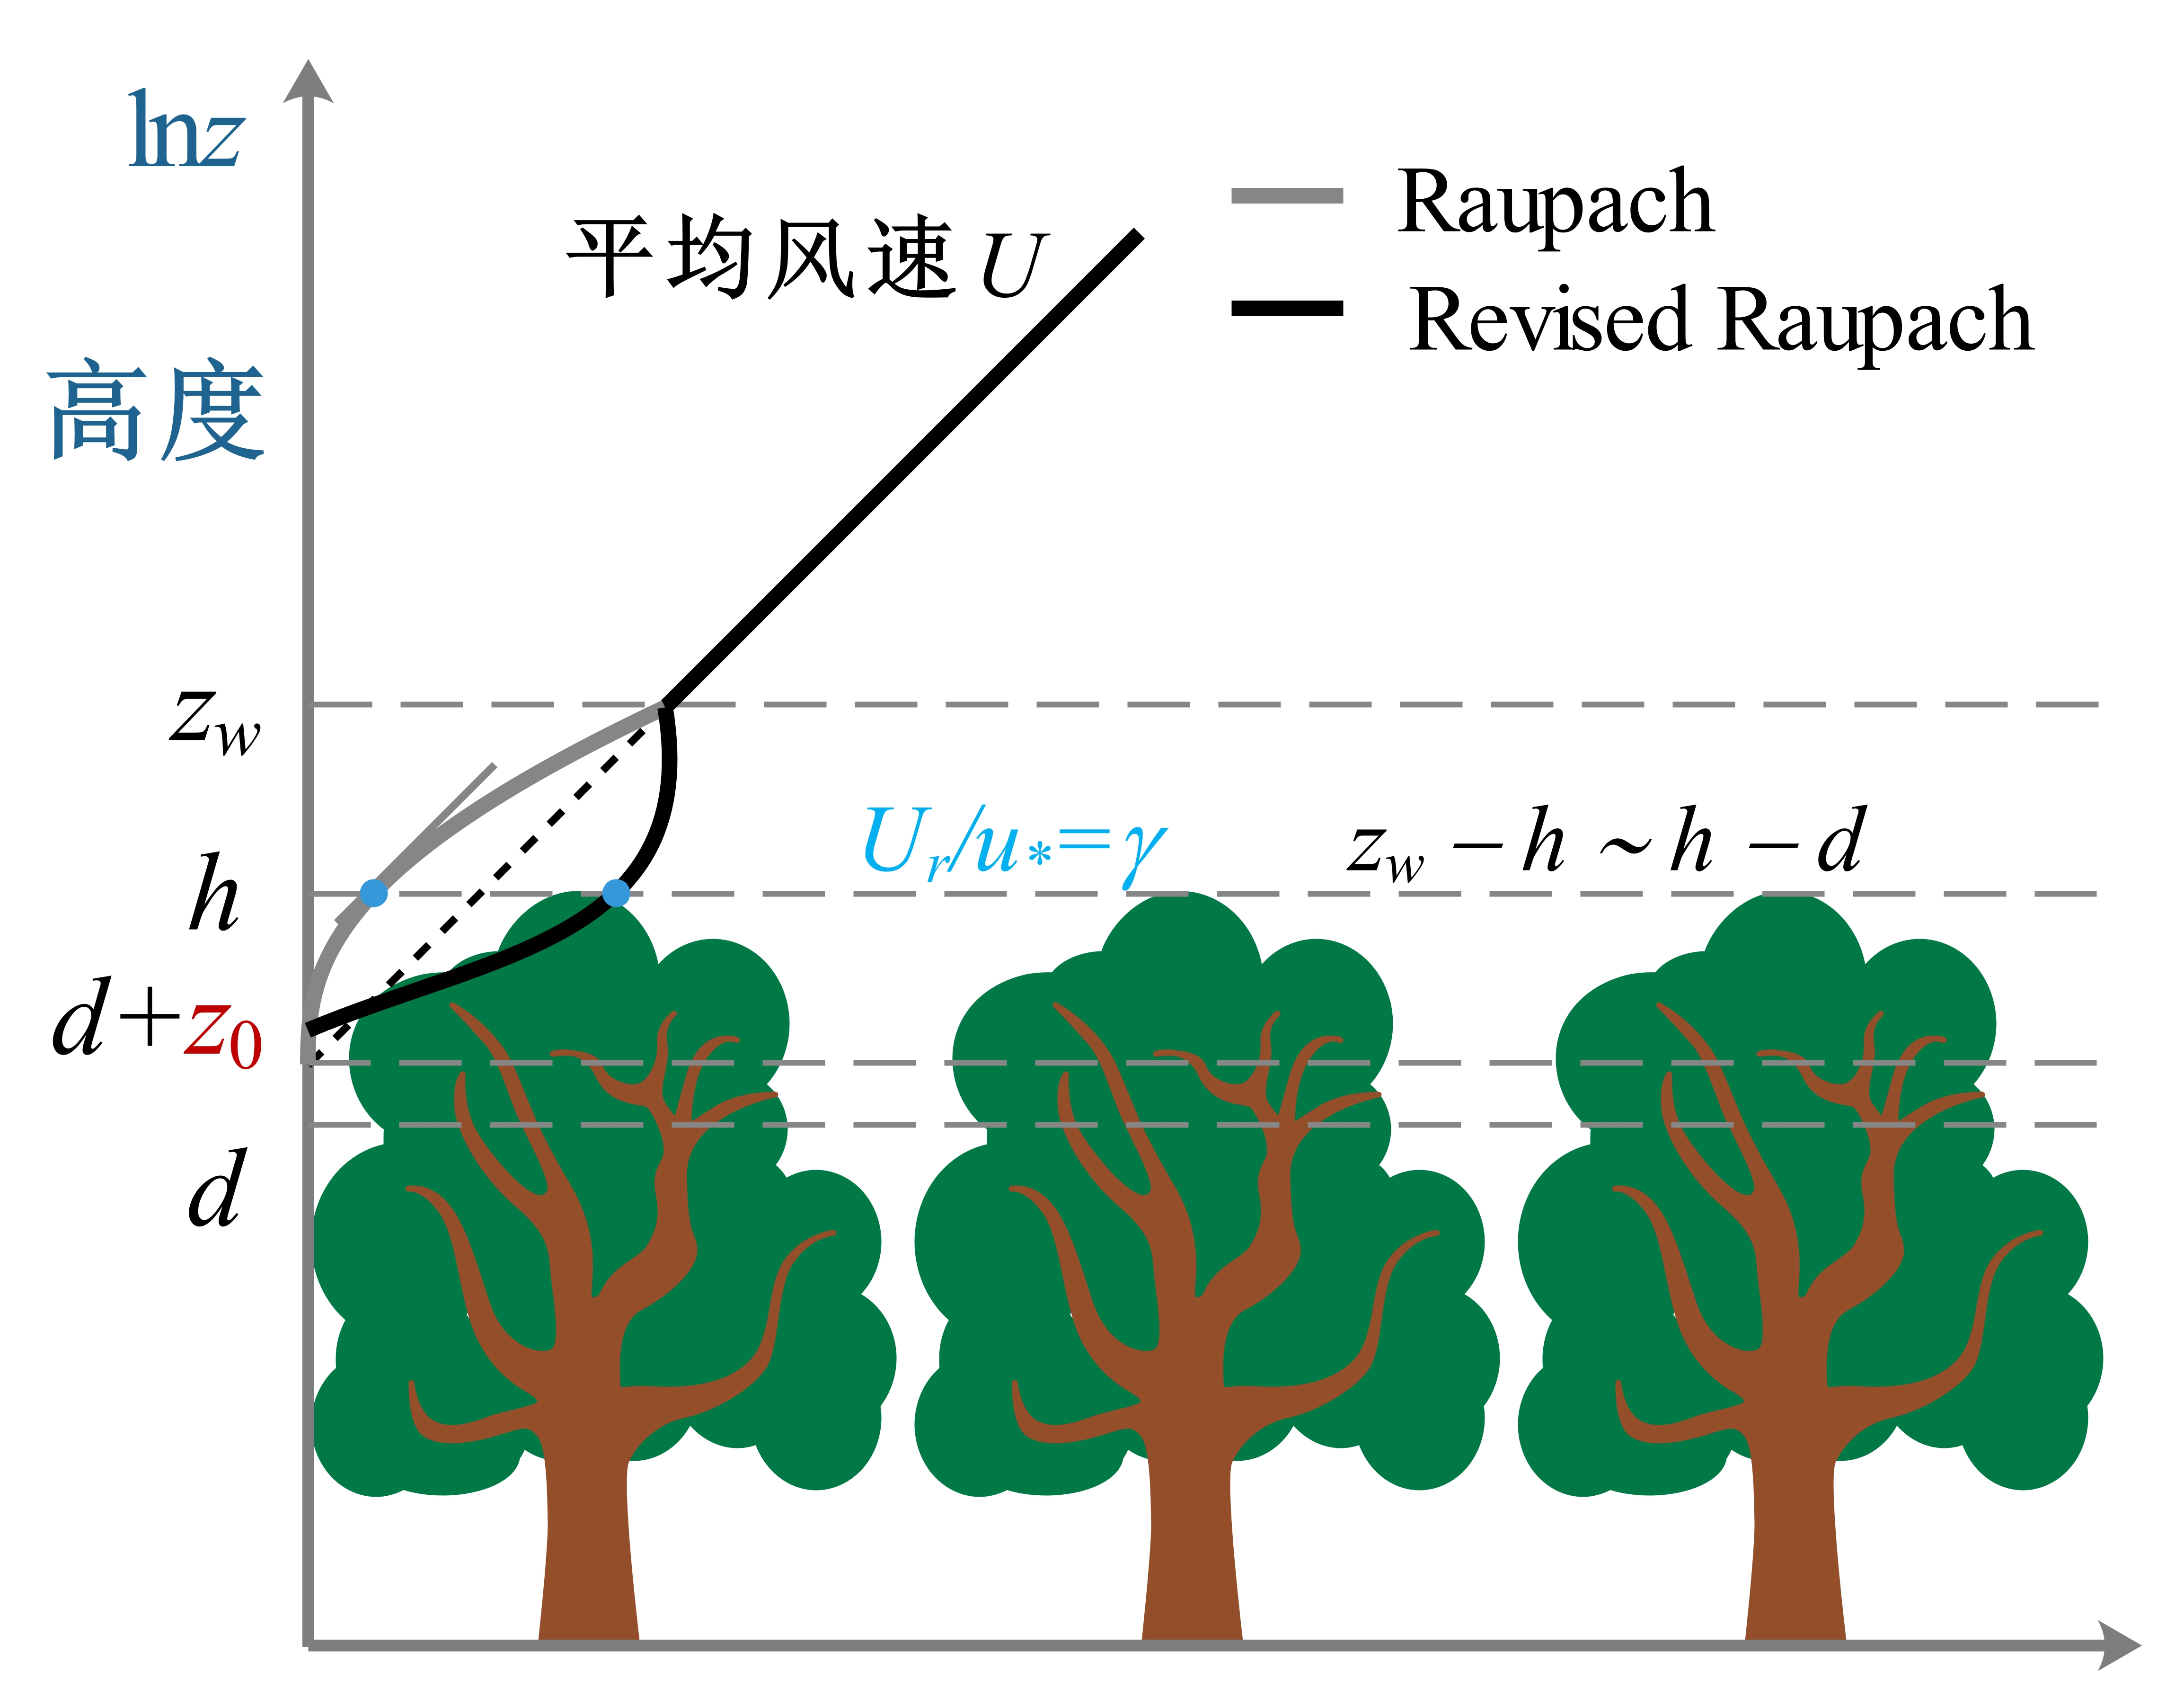
\includegraphics[scale=0.7]{Figures/地表湍流交换过程/修正Raupach粗糙度方案示意图.jpg}
\caption{考虑稳定度影响的植被粗糙度计算方案意图。}
\label{fig:修正Raupach粗糙度方案示意图}
\end{figure}
}


\subsection{单层植被湍流交换}
单层植被不同于100\%植被覆盖假设,而是考虑植被树冠之间可能存在空隙,
即植被树冠存在一定的水平分布,树冠覆盖度可介于0$\sim$100\%之间。这种植被结果假设与三维植被辐射模型假设一致。


对于植被树冠稀疏覆盖时,\citet{raupach1992drag,raupach1994simplified}通过场外和风洞实验,发展了一套用于计算$z_0$和$d$的解析解,其中:
\begin{equation}\label{dooh0}
\frac{d}{h}=1-\frac{1-\exp \left(-\sqrt{c_{d1} 2 \lambda}\right)}{\sqrt{c_{d1} 2 \lambda}}
\end{equation}
其中$c_{d1}=7.5$,$\lambda$%表示植被迎风面积指数 ($FAI$),
计算为$f_c\left(1-\exp{\left(-0.5LSAI\right)}\right)$。
当植被覆盖$f_c$等于100\%时,$\lambda$计算同100\%植被覆盖情景。为了同时适用与稀疏和浓密覆盖植被,
本版本采用\citet{dai2019different}方案计算$d$:
\begin{equation}\label{dooh}
\frac{d}{h}=f_{c} \cdot 1.1 \ln \left(1+\left(c_{d} f_{c} LAI\right)^{0.25}\right)+\left(1-f_{c}\right) \cdot\left(1-\frac{1-\exp \left(-\sqrt{c_{d1} 2 \lambda}\right)}{\sqrt{c_{d1} 2 \lambda}}\right)
\end{equation}
$z_0$的计算同公式 (\ref{zOh})。从上式可以看出,$d$值是100\%植被覆盖情景和稀疏植被按照植被覆盖度$f_c$的加权平均,
当$f_c\rightarrow100\%$时,公式 (\ref{dooh}) 趋同于公式 (\ref{dOh});当$f_c\rightarrow0\%$时,趋同于公式 (\ref{dooh0})。


对于植被冠层内的风速廓线$u$和湍流交换系数$K$,同样采用$f_c$加权方式。$u$和$K$分别计算为:
\begin{equation}
u(z)=f_{c} \cdot \min \left(u_{\exp }(z), u_{comb}(z)\right)+\left(1-f_{c}\right) \cdot u_{comb}
\end{equation}
\begin{equation}
\frac{1}{K(z)}=f_{c} \cdot \frac{1}{\min \left(K_{\exp}(z), K_{comb}(z)\right)}+\left(1-f_{c}\right) \cdot \frac{1}{K_{comb}}
\end{equation}
$u_{comb}$和$K_{comb}$同公式 (\ref{ucomb}) 和 (\ref{kcomb})。


\subsection{多层植被湍流交换}
多层植被湍流计算是以单层植被计算为基础,总体阻抗网络如图~\ref{fig:三层植被湍流交换示意图}所示。
风速$u$和湍流交换系数$K$廓线从最上层植被往下进行计算。上一层底部的廓线值作为下层植被顶部的值。
$r_b$和$r_d$的计算都是对$u$和$K$廓线的积分。
但积分区间对应到每层植被的等效交换高度(图~\ref{fig:三层植被湍流交换示意图} 中$T_{s1}$、$T_{s2}$、$T_{s3}$位置所示)。
该交换高度计算为该层植被100\%覆盖时的$d+z_0$值。在每一层等效交换高度,建议通量(感热H和潜热$\lambda E$)守恒方程,
即该点与上层通量交换量等于下层交换量加上该层植被的通量交换量。联立每层在等效高度建立的方程,迭代求解每种植被叶片温度。
{
\begin{figure}[]
\centering
\includegraphics{Figures/地表湍流交换过程/三层植被湍流交换示意图.png}
\caption{三层植被湍流交换示意图。}
\label{fig:三层植被湍流交换示意图}
\end{figure}
}


通过以上介绍可以看出,三维植被湍流交换与一维植被湍流交换最大的不同在于其计算的对象由原来单一植被扩展到多个分层植被,
阻抗网络发生变化,多种植被在同一环境下同时求解。在计算时,同一维植被一样,需要用到植被短波辐射吸收量和长波辐射吸收量,
此时利用章节~\ref{三维植被辐射传输模型} 和 \ref{三维植被长波辐射传输} 对三维植被辐射传输计算结果。整个植被冠层与大气的湍流交换同样采用相似性理论进行求解,
其求解过程如图~\ref{fig:三维植被湍流交换模型计算流程图} 所示。
{
\begin{figure}[htbp]
\centering
\includegraphics{Figures/地表湍流交换过程/三维植被湍流交换模型计算流程图.png}
\caption{三维植被湍流交换模型计算流程图。}
\label{fig:三维植被湍流交换模型计算流程图}
\end{figure}
}

\chapter{光合作用和气孔导度}
%\addcontentsline{toc}{chapter}{光合作用和气孔导度}

%\begin{光合作用和气孔导度}

\section{植物的光合作用}\label{植物的光合作用}
C3植物的光合作用模拟是基于Farquhar光合作用模型~\citep{farquhar1980biochemical},
C4植物则是基于~\citet{collatz1992} 的光合作用改进模型。
光合作用受到三方面的限制,即RuBP羧化酶的限制,RuBP再生速率的限制和羧化产物速率的限制,相应的受限羧化速率分别为:$A_{c}$, $A_{j}$, $A_{e}$。叶片净光合作用速率 ($A_{n}$) 等于受限光合羧化速率减去叶呼吸速率 ($R_d$):
\begin{equation}\label{An1}
A_{n}=\min \left(A_{c}, A_{j}, A_{e}\right)-R_{d}
\end{equation}


RuBP羧化酶限制主要指当羧化酶浓度不足时,光合作用最大羧化速率$V_{c \max }$受限。RuBP羧化酶限制下的最大羧化率 ($A_c$) 可表达为$V_{c \max }$的函数,其中C3植物羧化速率受到胞间CO$_2$分压$c_i$的调节,并表达为Michaelis-Menten函数:
\begin{equation}\label{A_C1}
A_{c}=\begin{cases}
\frac{V_{c \max }\left(c_{i}-\Gamma\right)}{c_{i}+K_{c}\left(1+\frac{o_{i}}{K_{o}}\right)}
     & \text{for C3 plants} \\ 
V_{c \max } & \text{for C4 plants}
\end{cases}
\end{equation}
其中,$\Gamma$是CO$_2$补偿点,$K_c$和$K_o$分别是对于CO$_2$和O$_2$的Michaelis--Menten常数(Pa),$o_i$是氧气分压(Pa)。\\
C3植物:\\
\begin{equation}\label{V_cmax_a}
V_{c \max }\left(T_{{leaf }}\right)=V_{c \max 25} \cdot \frac{2.1^{\frac{T_{{leaf }}-T_{o p}}{10}}}{1+e^{s_{1}\left(T_{{leaf }}-T_{{high }}\right)}} \cdot \beta
\end{equation}
C4植物:\\
\begin{equation}\label{V_cmax_b}
V_{c \max }\left(T_{{leaf }}\right)=V_{c \max 25} \cdot \frac{2.1^{\frac{T_{{leaf }}-T_{o p}}{10}}}{\left(1+e^{s_{2}\left(T_{{low }}
 - T_{{leaf }}\right)}\right)\left(1+e^{s_{1}\left(T_{{leaf }}-T_{h i g h}\right)}\right)} \cdot \beta
\end{equation}
$V_{c \max 25}$ 是 25 \textcelsius 下的最大羧化速率,单位: \unit{mol.m^{-2}.s^{-1}};$T_{op}$是参考温度298 K;$s_1$和$s_2$分别为高温和低温的温度敏感性参数;$T_{low}$和$T_{high}$分别为羧化速率的低温和高温响应参数,
取值根据植被类型而变化,范围分别为: 278$\sim$288 K,303$\sim$313 K;$T_{leaf}$是叶片温度,通过对叶片能量平衡方程进行牛顿迭代方法而求解得到,详见章节~\ref{植被叶片温度计算},$\beta$是植物水分胁迫因子,取值范围0$\sim$1,详见章节~\ref{气孔导度的水分胁迫}。

当光照不足时,RuBP再生速率下降,成为制约光合作用开尔文循环的最主要因素。因此,RuBP再生速率限制下的羧化速率 ($A_j$) 可表达为有效光合辐射 ($PAR$) 的函数:
\begin{equation}\label{A_J1}
A_{J}=\begin{cases}\frac{J_x\left(PAR\right)\left(c_{i}-\Gamma\right)}{4c_{i}+8\Gamma}
     & \text{for C3 plants} \\
\alpha\left(4.6\phi\right) & \text{for C4 plants}
\end{cases}
\end{equation}

$J_x$是有效光合辐射(PAR)的函数,并受叶片温度 ($T_{leaf}$) 的调节:
\begin{equation}
J_{x}\left(T_{{leaf }}\right)=\min \left(\alpha\left(4.6 \times 10^{-6} \cdot PAR\right), J_{\max 25}
 \cdot e^{\frac{37000\left(T_{{leaf }}-T_{o p}\right)}{T_{o p} \cdot T_{{leaf }} \cdot R} \cdot \frac{1+e^{\frac{710 \cdot T_{o p}-220000}
 {R \cdot T_{o p}}}}{\frac{710 \cdot T_{{leaf }}-220000}{R \cdot T_{{leaf }}}}}\right) \cdot \beta
\end{equation}
其中$\alpha$是量子效率 (\qty{0.05}{mol.CO_2.mol^{-1}.photon});$PAR$是有效光合辐射,单位: \unit{W.m^{-2}},详细计算见章节~\ref{短波吸收辐射通量};
\num{4.6e-6} 代表单位从 \unit{W.m^{-2}} 转换到 \unit{mol.photon.m^{-2}} 的转换系数;
$J_{\max 25}$是25 \textcelsius 下的最大电子传输速率,单位: \unit{mol.m^{-2}.s^{-1}},$J_{\max 25}=1.97 \cdot V_{c \max 25}$; 
$R$是通用气体常数,$R=$ \qty{8.314467591}{mol.m^{-2}.s^{-1}}。

羧化产物速率限制下的羧化速率 ($A_e$) 是25 \textcelsius 最大羧化速率常数 ($V_{c \max}$) 的函数,并且受到叶温和水分胁迫因子的调控:、\\
C3植物:\\
\begin{equation}\label{A_e_a}
A_e=\frac{V_{c \max 25}}{2} \cdot \frac{1.8^{\frac{T_{{leaf }}-T_{o p}}{10}}}{1+e^{s_{2}\left(T_{{leaf }}-T_{{low }}\right)}} \cdot \beta
\end{equation}
C4植物:\\
\begin{equation}\label{A_e_b}
A_e=\frac{V_{c \max 25}}{5} \cdot 1.8^{\frac{T_{{leaf }}-298.16}{10}} \cdot \beta
\end{equation}
三方面限制下的羧化速率均共用同一套温度响应常数 ($T_{op}$,$T_{low}$和$T_{high}$)


呼吸速率对温度的响应曲线可表示为$V_{c \max25}$的函数:
\begin{equation}\label{R_d1}
R_{d}=r_{{base }} \cdot V_{cmax 25} \cdot \frac{2.0^{\frac{T_{leaf}-T_{op}}{10}}}{1+e^{s_3 \cdot\left(T_{leaf}-T_{d m}\right)}} \cdot \beta
\end{equation}
其中$T_{dm}$是叶呼吸的高温抑制温度常数,单位 K。



在求解最小值的计算中,我们将三值最小问题的求解拆分为两个二值最小问题的求解:
\begin{equation}\label{min_Ac_Aj_Ae}
\min \left(A_{c}, A_{j}, A_{e}\right)=\min \left(\min \left(A_{c}, A_{j}\right), A_{e}\right)
\end{equation}
引入形状参数$\theta$,构造一元二次方程,将求解最小值问题转换成求一元二次方程较小根的问题,以此避免模拟中不同光合限制之间过渡转换时的光合同化速率突变 \citep{collatz1991,collatz1992}:
\begin{equation}\label{theta_cj}
\theta_{c j} \cdot A_{i1}^{2}-\left(A_{c}+A_{j}\right) A_{i1}+A_{c} A_{j}=0
\end{equation}
\begin{equation}\label{theta_cje}
\theta_{c j e} \cdot A_{i2}^{2}-\left(A_{i1}+A_{e}\right) A_{i2}+A_{i1} A_{e}=0
\end{equation}
其中形状参数$\theta_{cj}=0.877$,$\theta_{cje}=0.95$。$A_{i1}$为方程(\ref{theta_cj})的较小根,代表$A_c$和$A_j$的最小值。$A_{i2}$为方程(\ref{theta_cje})的较小根,代表$A_{i1}$和$A_e$的最小值。


\section{气体扩散方程和气孔导度模型}\label{气体扩散方程和气孔导度模型}
气孔是植被和大气相互作用的最重要通道,光合作用速率和蒸腾速率的计算与气孔导度紧密结合,并遵循气体扩散方程,刻画了从叶片细胞间到大气$\rm CO_2$浓度和水汽浓度梯度的重要影响~\eqref{A_n2},~\eqref{ea_ei}。我们通过分别模拟叶绿体细胞间、叶表和冠层大气中的大气$\rm CO_2$浓度和水汽浓度来表现其梯度,如图~\ref{fig:叶片气孔光合作用导度模型示意图}:

{
\begin{figure}[]
\centering
\includegraphics{Figures/气孔导度和光合作用/叶片气孔光合作用导度模型示意图.png}
\caption{叶片气孔光合作用导度模型示意图。}
\label{fig:叶片气孔光合作用导度模型示意图}
\end{figure}
}


\begin{equation}\label{A_n2}
A_{n}=\left(c_{a}-c_{s}\right) /\left(\frac{1.37}{g_{b}} p_{s}\right)=\left(c_{s}-c_{i}\right) /\left(\frac{1.6}{g_{s}} p_{s}\right)
\end{equation}
\begin{equation}\label{ea_ei}
\left(e_{a}-e_{i}\right) /\left(\frac{1}{g_{b}}+\frac{1}{g_{s}}\right)=\left(e_{s}-e_{i}\right) / \frac{1}{g_{s}}
\end{equation}
其中,$c_i$是胞间CO$_2$分压,$c_s$是叶表CO$_2$分压,$c_a$是冠层大气$\rm CO_2$分压,叶表水汽分压$e_s$,$e_a$是冠层大气水汽分压,$e_i$是胞间水汽分压,单位: Pa,$g_b$是叶片边界层导度,$g_s$是叶片气孔导度,单位: \unit{mol.m^{-2}.s^{-1}};单位: Pa。

气孔导度理论认为植被根据自身光合同化速率、环境大气水分亏缺以及土壤水分胁迫等因素,主动调控气孔导度。CoLM的气孔导度计算沿用Ball-Berry模型,Ball-Berry模型根据叶片净光合作用速率 
($A_n$,单位: \unit{mol.CO_2.m^{-2}.s^{-1}})、叶表水汽压 ($e_s$,单位: Pa)、叶表二氧化碳分压 ($c_s$,单位: Pa) 
基于气孔导度的观测回归经验关系,计算气孔导度 ($g_s$, 单位: \unit{mol.CO_2.m^{-2}.s^{-1}}): 
\begin{equation}\label{rs_a1}
\frac{1}{r_{s}}=g_{s}=m \frac{A_{n}}{c_{s}} \frac{e_{s}}{e_{i}} p_{s}+b\beta
\end{equation}
$r_s$代表叶片气孔阻抗,单位: \unit{s.m^{-1}},是气孔导度$g_s$的倒数;$m$是无量纲经验参数;$b$是最小气孔导度,
单位: \unit{mol.CO_2.m^{-2}.s^{-1}},$m$和$b$是观测拟合的经验系数;$e_i$是饱和水蒸气压,
是气温的函数,单位: Pa;$p_s$是大气压强,单位: Pa,$\beta$是植物水分胁迫因子,取值范围0$\sim$1。


气孔行为的预测需要综合考虑植被自身的光合能力,大气$\rm CO_2$浓度梯度,水汽浓度梯度和土壤水分胁迫,因此,需要联立光合作用模块方程、气体扩散方程,气孔导度模型和土壤水分胁迫方案,求解叶片气孔导度。
由方程~\eqref{A_n2} 可知:
\begin{equation}\label{cs_a1}
c_{s}=c_{a}-\frac{1.37 A_{n}}{g_{b}} p_{s}
\end{equation}
由方程~\eqref{ea_ei} 可知:
\begin{equation}\label{e_s1}
e_{s}=\left(\frac{e_{a}}{g_{s}}+\frac{e_{i}}{g_{b}}\right) /\left(\frac{1}{g_{b}}+\frac{1}{g_{s}}\right)
\end{equation}
将方程~\eqref{e_s1} 代入方程~\eqref{rs_a1}中,得到关于$g_s$的一元二次方程:
\begin{equation}\label{ei_cs}
\frac{e_{i} c_{s}}{m A_{n} p_{s}} g_{s}^{2}+\left(g_{b} \frac{e_{i} c_{s}}{m A_{n} p_{s}}-e_{i}-b \beta \frac{e_{i} c_{s}}{m A_{n} p_{s}}\right) g_{s}
-\left(e_{a} g_{b}+b \beta g_{b} \frac{e_{i} c_{s}}{m A_{n} p_{s}}\right)=0
\end{equation}
气孔导度 ($g_s$) 的解即为一元二次方程的正根,其中叶片表层$\mathrm{CO_2}$分压 ($c_s$) 由方程~\eqref{cs_a1} 得出,$A_n$由光合作用模块公式~\eqref{An1} 得出,
但仍然包含未知变量胞间 $\mathrm{CO_2}$ 分压 ($c_i$),完整求解光合气孔模式还需根据~\eqref{A_n2} 得出:
\begin{equation}\label{ci_1}
c_{i}=c_{s}-\frac{1.6 A_{n} p_{s}}{g_{s}}
\end{equation}
联立~\eqref{An1}, \eqref{cs_a1}, \eqref{ei_cs} 和 \eqref{ci_1} 可以求解 $g_s$,$c_i$,$c_s$ 和 $A_n$。
通过牛顿迭代数值解法 (章节~\ref{数值计算方案}),对胞间$\mathrm{CO_2}$分压 $c_i$ 求解,从而求解所有未知量。


\chapter{植被水力模式}
%\addcontentsline{toc}{chapter}{植被水力模式}

%\begin{植被水力模式}
CoLM植物水力模式根据土壤-植物-大气连通体的概念计算陆气水分交换的蒸腾分量。
CoLM植物水力模式中的植物水分传输得益于土壤、根、茎和叶之间形成的水势梯度。植物各部位的水势也密切影响着各植物水力过程。
首先,根、茎、叶的水势通过植物栓塞过程影响着植物水分传输能力 (详见章节 \ref{植物水力导度的衰减})。
其次,植物根与每层土壤的水势梯度将影响根的水力重分配过程 (详见章节 \ref{地下植物水力过程})。最后,叶片的水势降低将影响叶片气孔导度,
同时影响植物水分传输和光合作用 (详见章节 \ref{气孔导度的水分胁迫})。


\section{植物水势动态}\label{植物水势动态}
植物水势的动态模拟是CoLM植物水力模式的关键。CoLM植物水力模式的水势模拟包括地上和地下植物水力过程两部分
。地上部分包括在阳叶、阴叶、茎和地表根四个节点的水势 ($\Psi_{sunleaf}$,$\Psi_{shaleaf}$,$\Psi_{stem}$,$\Psi_{root,0}$)

 模拟;地下部分包括地表根以及$n$层地下根 $n+1$个节点的水势 ($\Psi_{root,i}$,$i=0,1,2,\ldots,n$) 模拟。地上、地下两部分通过地表根水势
 ($\Psi_{root,0}$)的模拟被密切的耦合(如图~\ref{fig:CoLM植物水力模型示意图})。

 {
\begin{figure}[htbp]
\centering
\includegraphics{Figures/植被水力模式/CoLM植物水力模型示意图.png}
\caption{CoLM植物水力模型示意图。}
\label{fig:CoLM植物水力模型示意图}
\end{figure}
}


CoLM植物水势的动态模拟假设植物水分传输为稳恒流,并将其类比为电路问题~
\citep{van1948water},即水分传输速率正比于水势差和水力导度。
地上部分四个节点的水势由Darcy定律表达,满足以下方程:
\begin{equation}\label{q_sunstem}
q_{ {sun \leftarrow stem }}=k_{{sun} \leftarrow  {stem}}\left(\Psi_{sunleaf}-\Psi_{stem}\right)
\end{equation}
\begin{equation}
q_{ {sha \leftarrow stem }}=k_{ {sha} \leftarrow {stem}}\left(\Psi_{shaleaf}-\Psi_{ {stem }}\right)
\end{equation}
\begin{equation}
q_{ {stem \leftarrow root }}=k_{ {stem } \leftarrow  { root }}\left(\Psi_{ {stem }}-\Psi_{ {root }, 0}\right)
\end{equation}
$k_{sun \leftarrow stem}$,$k_{sha \leftarrow stem }$,$k_{stem \leftarrow root }$ 分别代表茎到阳叶的水力导度、茎到阴叶的水力导度和根到茎的水力导度。
水力导度随水势降低而降低,是关于茎和根水势的函数 (详见章节~\ref{植物水力导度的衰减}) 。地表根水势$\Psi_{root,0}$是关于每层土壤水势 ($\Psi_{soil,i}$) 
及根总吸水速率 ($q_{root,0}$) 的函数,由地下植物水力过程所计算 (详见章节~\ref{地下植物水力过程}):
\begin{equation}\label{Psi_root_0}
\Psi_{root, 0}=R\left(\Psi_{ {soil }, i}, q_{root, 0}\right)
\end{equation}
$q_{sun \leftarrow stem}$,$q_{sha \leftarrow stem }$,$q_{stem \leftarrow root }$分别代表茎到阳叶的水流速、茎到阴叶的水流速和根到茎的水流速。
水流速在各节点由于稳恒流假设,满足水分守恒方程:
\begin{equation}
E_{sun}=q_{sun \leftarrow  stem}
\end{equation}
\begin{equation}
E_{ {sha }}=q_{ sha \leftarrow stem}
\end{equation}
\begin{equation}
q_{ {sun \leftarrow stem }}+q_{ {sha \leftarrow stem }}=q_{ {stem \leftarrow root }}
\end{equation}
\begin{equation}\label{q_stemroot}
q_{stem \leftarrow root}=q_{root, 0}
\end{equation}
$E_{sun}$代表阳叶蒸腾速率,$E_{sha}$代表阴叶蒸腾速率。它们是由无水分胁迫情况下的叶片蒸腾 ($E_{sun,max}$, $E_{sha,max}$) 
和受叶片水势 ($\Psi_{sunleaf}$,$\Psi_{shaleaf}$) 控制的蒸腾衰减函数所组成(详见章节~\ref{植物水力导度的衰减})。
同时,无水分胁迫的叶片蒸腾是在最大气孔导度 ($g_{s,sun,max}$, $g_{s,sha,max}$) 的条件下,
运用章节~\ref{一维植被湍流交换模型} 植被覆盖地表湍流通量的计算方案所推导得出。最大气孔导度的计算则需要植物水力模式、光合作用模式、气孔导度模式耦合解出 (详见章节~\ref{气体扩散方程和气孔导度模型})。


\section{植物水力导度的衰减}\label{植物水力导度的衰减}
植物水势下降导致的空穴现象会严重降低水分在植物内部的传导能力。我们将实验上观测到水力导度随水势变化的S型脆弱性曲线 
\citep{sperry1988method,gentine2016allometry,neufeld1992genotypic,pammenter1998mathematical,plaut2012hydraulic}
 引入到模型,对植物水力栓塞进行参数化,得到节点间的水力导度$k_{i\gets j}$ (从节点$j$到$i$的传输):
\begin{equation}
k_{i \leftarrow j}=k_{\max } \cdot 2^{-\left(\frac{\Psi_{\mathbf{j}}}{p 50}\right)^{c_{k}}}
\end{equation}
其中$k_{max}$表示最大水力导度 (\unit{s^{-1}})。$\Psi_j$代表节点$j$的水势 (\unit{mm.H_2O}),$p50$代表水力导度降低 50\% 时的水势 (\unit{mm.H_2O}),$c_k$代表脆弱性曲线的形状参数。


实验数据发现气孔导度和叶片水势同样存在S型曲线关系 \citep{klein2014variability},
CoLM植物水力模式引入蒸腾速率随叶片水势 ($\Psi_{sunleaf}$,$\Psi_{shaleaf}$)的衰减函数 \citep{kennedy2019implementing}:
\begin{equation}\label{e_sun_a}
E_{ {sun }}=E_{ {sun,max }} \cdot 2^{-\left(\frac{\Psi_{ {sunleaf }}}{p 50}\right)^{c_{k}}}
\end{equation}
\begin{equation}\label{e_sha_a}
E_{ {sha }}=E_{ {sha,max }} \cdot 2^{-\left(\frac{\Psi_{ {shaleaf }}}{p 50}\right)^{c_{k}}}
\end{equation}
$E_{sun,max} $和$E_{sha,max}$分别表示无水分胁迫情况下的阳叶、阴叶的最大蒸腾速率。


\section{地下植物水力过程}\label{地下植物水力过程}
水力重分配是重要的植物地下水力过程,它描述了水分通过地下根系从湿润土壤层向干燥土壤层的传输。
它被认为是一个被动的受水势梯度所驱动的水分传输过程。基于该物理原理,Amenu水力重分配模型 \citep{amenu2008}被CoLM采用 \citep{zhu2017incorporating},
并与土壤水文过程和植被地上水力过程相耦合 \citep{li2021new},考虑包括在根、茎和叶等地上节点外的, 
$n$个代表不同土壤深度的根系水力节点和$n$个土壤水力节点 (如图~\ref{fig:CoLM植物水力模型示意图})。模式中的水力传导包括轴向水力传导和径向水力传导。
轴向水力传导由Darcy定律所表示:
\begin{equation}\label{k_axi}
k_{ax,i}\left(\Psi_{r,i}-\Psi_{r,i+1}\right)=q_{ax,i}
\end{equation}
其中$k_{ax,i}$代表第$i+1$层到第i层根节点间的轴向水力导度,$q_{ax,i}$代表相应的轴向水分传输速率,
$\Psi_{r,i}$代表第$i$层根节点的水势。$i$取值1到$n-1$,$n$代表土壤总层数。\\
径向水力传导方程:
\begin{equation}\label{k_radi}
k_{rad,i}\left(\Psi_{soil,i}-\Psi_{r,i}\right)=q_{rad,i}
\end{equation}
其中$k_{rad,i}$代表第$i$层土壤节点到根节点间的径向水力导度,
$q_{rad,i}$代表相应的径向水分传输速率,$\Psi_{soil,i}$代表第$i$层土壤节点的水势,$i$取值1到$n$。



对于第2到$n$层的土壤根节点存在水分平衡方程:
\begin{equation}\label{q_axi}
q_{a x, i}+q_{r a d, i}=q_{a x, i-1}
\end{equation}
其中$i=2, \ldots, n$,方程~\eqref{q_axi} 实际上是$n-1$个方程组。


另外,由表层根节点的水分平衡方程可得:
\begin{equation}\label{q_ax1}
q_{ax,1}+q_{rad, 1}=q_{root,0}
\end{equation}
将方程(\ref{k_axi})和(\ref{k_radi})代入(\ref{q_axi})和(\ref{q_ax1}),则得到关于$ \Psi_{r,i}$的$n$个线性方程组。
这$n$个线性方程组描述了在植物地下水力过程作用下,根水势垂直分布。其输入包括土壤水势垂直分布 ($\Psi_{soil,i}$) 和根总吸水速率 ($q_{root,0}$)。
其输出包括根水势垂直分布 ($\Psi_{r,i}$) 和根吸水速率垂直分布 ($q_{rad,i}$)。因此,地下植物水力过程可以被简化地表示为公式(\ref{Psi_root_0})。


\section{气孔导度的水分胁迫}\label{气孔导度的水分胁迫}
土壤水分亏缺对植物生理的影响被表现在水分胁迫因子上,水分胁迫因子作为取值 $0\sim 1$ 的无量纲变量,作用在光合作用各限制因子上,见公式(\ref{V_cmax_a})--(\ref{R_d1})。

植物水力模式未开启时,水分胁迫因子 ($\beta$) 决定于根的垂直分布比例和土壤水势,其计算不区分阴叶和阳叶:
\begin{equation}\label{beta_0}
\beta=\sum_{i=1}^{n} froot_i \beta_{i}
\end{equation}

\begin{equation}\label{beta_i}
\beta_{i}=\frac{\Psi_{\max }-\Psi i}{\Psi_{\max }-\Psi_{s a t}}
\end{equation}
$froot_i$是第i层的根含量,$\beta_i$是第$i$层的水分胁迫因子;它根据每层土壤的实际水势 (${\Psi}_i$),最大水势 (${\Psi}_{max}$)和饱和水势 (${\Psi}_{sat}$)计算得出。

当植物水力模式开启时,水分胁迫对植被的直接影响是植物水势的降低,气孔通过关闭以尽量保持植物的导水能力,但同时也导致叶片光合速率降低。
植物水力模式符合植物生理学理论和物理规律,水分胁迫因子 ($\beta_{sun}$,$\beta_{sha}$) 决定于气孔导度的衰减比例,其计算区分阳叶和阴叶:
\begin{equation}\label{beta_sun}
\beta_{sun}=g_{s,sun} / g_{s,sun,max }
\end{equation}
\begin{equation}\label{beta_sha}
\beta_{sha}=g_{s,sha} / g_{s,sha, \max }
\end{equation}
$g_{s,sun}$和$g_{s,sun}$分别代表阳叶和阴叶的实际气孔导度,
$g_{s,sun,max}$和$g_{s,sun,max}$分别代表阳叶和阴叶在无水分胁迫条件下的最大气孔导度。
水分胁迫的求解需要耦合地表冠层湍流参数化方案和光合气孔模式。


最大气孔导度 ($g_{s,sun,max}$和$g_{s,sun,max}$) 的计算依赖于光合气孔模式。
光合气孔模式中,气孔导度为方程(\ref{ei_cs})的正根,(\ref{ei_cs})和(\ref{ci_1})联立可表示为实际气孔导度关于净光合作用速率的隐式方程:
\begin{equation}\label{gs_0}
g_{s}=g\left(A_{n}\right)
\end{equation}
由于水分胁迫是光合作用中的相关参数,公式(\ref{gs_0})可以写成:
\begin{equation}\label{gs_1}
g_{s}=g\left(f_{photo}(\beta)\right)
\end{equation}
最大气孔导度可表述为:
\begin{equation}\label{gs_sunmax}
g_{s,  { sun,max }}=\frac{g\left(f_{ {photo }}\left(\beta_{ {sun }}\right)\right)}{\beta_{ {sun }}}
\end{equation}
\begin{equation}\label{gs_shamax}
g_{s, sha, \max }=\frac{g\left(f_{photo}\left(\beta_{s h a}\right)\right)}{\beta_{s h a}}
\end{equation}
$f_{photo}$代表公式(\ref{An1})的光合作用模型。


最大气孔导度一方面是植物水力模式水分胁迫计算的必要变量(公式(\ref{beta_sun})和(\ref{beta_sun})),
另一方面,为地表冠层湍流参数化方案中叶片最大蒸腾速率计算提供重要输入 (如图~\ref{fig:光合气孔模式和植物水力模式的耦合示意图})。
地表冠层湍流参数化方案中的叶片最大蒸腾速率$(E_{sun,max}$和$E_{sha,max}$) 可简化地表示为:
\begin{equation}\label{E_sunmax}
E_{sun, \max }=E\left(g_{s, sun, \max }\right)
\end{equation}
\begin{equation}\label{E_shamax}
E_{sha, \max }=E\left(g_{s, sha, \max }\right)
\end{equation}
其中,与植物水力模式无关的参数、变量在此省略,完整表述见植被覆盖地表湍流通量的计算方案 (见章节 \ref{一维植被湍流交换模型})。


实际气孔导度 ($g_{s,sun}$和$g_{s,sun}$) 的计算同样依赖于地表冠层湍流参数化方案。由于植物水力模式可以求解植物叶片实际蒸腾 ($E_{sun}$和$E_{sha}$),
可以利用公式(\ref{E_sunmax})和(\ref{E_shamax})的逆函数求解气孔导度:
\begin{equation}\label{g_ssun}
g_{s, s u n}=E^{-1}\left(E_{s u n}\right)
\end{equation}
\begin{equation}\label{g_ssha}
g_{s, sha}=E^{-1}\left(E_{s h a}\right)
\end{equation}
耦合植物水力模式、光合气孔模式和地表冠层湍流参数化方案,再利用公式(\ref{beta_sun})和(\ref{beta_sha})可以完整地求解植物水力模式下的植物水分胁迫 (如图 \ref{fig:光合气孔模式和植物水力模式的耦合示意图})。
{
    \begin{figure}[htbp]
    \centering
    \includegraphics{Figures/植被水力模式/光合气孔模式和植物水力模式的耦合示意图.png}
    \caption{光合气孔模式和植物水力模式的耦合示意图。}
    \label{fig:光合气孔模式和植物水力模式的耦合示意图}
    \end{figure}
}


\section{数值计算方案}\label{数值计算方案}
求解植物水势、水分胁迫、气孔导度和叶片蒸腾速率,需要耦合植物水力模式、光合气孔模式和地表冠层参数化方案。
耦合描述植物水势变化的动力方程组(公式(\ref{q_sunstem})--(\ref{q_stemroot}), (\ref{e_sun_a}) 和(\ref{e_sha_a})),
地表冠层参数化方案 (公式(\ref{E_sunmax})--(\ref{g_ssha})),
光合气孔模式的最大气孔导度计算 (公式(\ref{gs_sunmax})和(\ref{gs_shamax})), 植物水分胁迫计算(公式(\ref{beta_sun})和(\ref{beta_sha})),共18个方程,
求解包括4个植物地上水势节点 ($\Psi_{sunleaf}$, $\Psi_{shaleaf}$, $\Psi_{stem}$和$\Psi_{root,0}$),8个水分传输速率 
($q_{sun-stem}$,$q_{sha-stem}$,$q_{stem-root}$,$q_{root,0}$,$E_{sun}$,$E_{sun,max}$和$E_{sun,max}$) ,4个气孔导度变量
 ($g_{s,sun}$,$g_{s,sun}$,$g_{s,sun,max}$,$g_{s,sun,max}$),2个水分胁迫变量 ($\beta_{sun}$,$\beta_{sha}$) 在内的共18个未知量。

然而,由于以上18个方程中存在隐形方程,我们求解该问题时,引入三重嵌套数值求解办法。其主要步骤如下(图 \ref{fig:植物水力模式的数值模拟流程图}):
\begin{enumerate}
    \item 利用冠层模型,计算叶片温度 ($T_{l,sun}$,$T_{l,sha}$);
    \item 利用光合气孔模式,计算最大气孔导度 ($g_{s,sun,max}$和$g_{s,sun,max}$);
    \item 根据最大气孔导度,计算叶片最大蒸腾速率 ($E_{sun,max}$和$E_{sun,max}$);
    \item 将叶片最大蒸腾速率输入植物水力模式,计算水分胁迫 ($\beta_{sun}$,$\beta_{sha}$);
    \item 更新光合气孔模式的水分胁迫,迭代计算,判断胞间二氧化碳浓度是否收敛,若收敛,进入第 (6) 步;若不收敛,重复此步骤;
    \item 更新气孔导度,判断阴叶、阳叶水分胁迫是否收敛,若收敛,进入第 (7) 步,若不收敛,回到第 (2) 步;
    \item 更新植物水势和叶片蒸腾,判断叶片温度是否收敛,若收敛,植物水力模式求解完成,若不收敛,回到第 (1) 步。
\end{enumerate}

气孔导度详细迭代

{
    \begin{figure}[htbp]
    \centering
    \includegraphics{Figures/植被水力模式/植物水力模式的数值模拟流程图.png}
    \caption{植物水力模式的数值模拟流程图。}
    \label{fig:植物水力模式的数值模拟流程图}
    \end{figure}
}


\chapter{降水与地表的能量交换}
%\addcontentsline{toc}{chapter}{降水与地表的能量交换}

%\begin{降水与地表的能量交换}
雨水与地表/植被之间存在温度差异,当降水发生时,它们之间可发生能量交换(雨水感热)。
\citet{wei2014impact} 表明,虽然在气候尺度上此能量交换的量级很小,但它可通过改变大气环流影响不同地区的气候特征,
故在气候模式中不可被忽略。下面给出雨水感热的计算方案。
\begin{mymdframed}{代码}
本部分的对应代码为\texttt{groundtem.F90}、\texttt{rain\_snow\_temp.F90}和\texttt{wetbulb.F90}。
\end{mymdframed}


\section{雨水温度}\label{雨水温度}
已有研究(如\citet{anderson1998moored})表明,
雨水温度非常接近于大气湿球温度,故这里雨水温度由湿球温度近似。根据湿球温度定义有如下关系:
\begin{equation}
C_{p a}\left(T_{w b}-T\right)=\lambda_{v}\left(r-r_{s a t}^{T_{w b}}\right)
\end{equation}
其中 $C_{pa}$ 表示干空气的比热容 (\unit{J.kg^{-1}.K^{-1}}),$T_{wb}$ 表示大气湿球温度 (K),
$T$ 表示大气环境温度 (K),$r$ 表示混合比,$r_{sat}^{T_{wb}}$ 表示 $T_{wb}$ 温度下的饱和混合比,
$\lambda_v$ 表示液态水的蒸发潜热 (\unit{J.kg^{-1}})。于是,取 $T_{wb}$ 的初始值 $T_{wb}^{\left(0\right)}=T$,
$T_{wb}$ 可通过如下过程进行迭代求解:
\begin{enumerate}
    \item 由附录~\ref{饱和水汽压(比湿)及其随温度的变化} 计算$T_{wb}^{\left(n\right)}$温度下的饱和比湿$q_{sat}^{T_{wb}^{\left(n\right)}}$;
    \item 通过混合比和比湿的换算关系($r=\frac{q}{1-q}$),计算混合比$r$与$r_{sat}^{T_{wb}^{\left(n\right)}}$;
    \item 由上述关系更新湿球温度:$T_{wb}^{\left(n\right)\ast}=T+\frac{\lambda_v}{C_{pa}}\left(r-r_{sat}^{T_{wb}^{\left(n\right)}}\right)$;
    \item 取更新前后湿球温度的平均值作为新一步的湿球温度:$T_{wb}^{\left(n+1\right)}=\left(T_{wb}^{\left(n\right)}+T_{wb}^{\left(n\right)\ast}\right)/2.0$。
\end{enumerate}
将上述过程迭代6次($n=0$, $\ldots$, 5),作为最终的湿球温度$T_{wb}$。


当$T>T_f+2.5$ K时,降水完全为液态水,可取雨水温度$T_p=T_{wb}$,否则$T_p$需根据降水的固态与液态比例进行调整。
根据《Snow Hydrology》(1956)中的实验结果,液态水占总降水的比例$f_{pl}$可按如下方式定义:
\begin{equation*}
f_{pl}= \begin{cases}
0.4, & \text{当 }\ T_f+2.0\text{ K}<T\le T_f+2.5\text{ K} \text{ 时} \\
-54.632+0.2T, & \text{当 }\ T_f<T\le T_f+2.0\text{ K} \text{ 时} \\
0, & \text{当 }\ T\le T_f \text{ 时}
\end{cases}
\end{equation*}
于是,当$T\le T_f+2.5$ K 且$f_{pl}>0$时,$T_p=T_f-\sqrt{\frac{1}{f_{pl}}-1}/100$,
否则当降水完全为固态时,$T_p=\min{\left(T_f,T_{wb}\right)}$。


\section{植被/地表的雨水感热}\label{植被地表的雨水感热}
当地表有植被覆盖时,植被叶片与雨水的能量交换 (\unit{W.m^{-2}}) 分别计算如下:
\begin{equation}
H_{prcv}=C_{pl} q_{pl}\left(T_{p}-T_{v}\right)+C_{pi} q_{pi}\left(T_{p}-T_{v}\right)
\end{equation}
%
其中$C_{pl}$与$C_{pi}$分别表示液态水与固态水的比热容(\unit{J.kg^{-1}.K^{-1}}),
$q_{pl}$与$q_{pi}$分别表示植被冠层对液态水和固态水的截流率(\unit{mm.H_2O.s^{-1}})(计算见章节~\ref{植被冠层截留})。


地表与雨水的能量交换 (\unit{W.m^{-2}}) 为:
\begin{equation}
H_{p r c g}=C_{p l} p_{l}\left(T_{p}-T_{g}\right)+C_{p i} p_{i}\left(T_{p}-T_{g}\right)
\end{equation}
其中$p_l$与$p_i$分别表示落到地面的液态水与固态水降水率(\unit{mm.H_2O.s^{-1}}),
当有植被覆盖时,$p_l$与$p_i$为直接穿透植被冠层的降水率与沿叶茎流出冠层的降水率之和(计算见章节~\ref{植被冠层截留})。


\part{植被冠层、积雪和土壤温度计算方案}
\include{植被叶片温度计算/植被叶片温度计算}
\chapter{雪盖土壤热力过程}
%\addcontentsline{toc}{chapter}{雪盖土壤热力过程}

%\begin{雪盖土壤热力过程}

在雪盖和土壤中,热力过程主要根据热传导第二定律进行描述。假设雪盖土壤无水平物质能量交换,则其垂直方向上的一维能量平衡方程如下:
\begin{equation}\label{eq:1d_energy_balance}
c \frac{\partial T}{\partial t}=-\frac{\partial F}{\partial z}
\end{equation}
其中$c$表示雪盖或土壤的体积热容量(\unit{J.m^{-3}.K^{-1}}),$T$表示雪盖土壤温度 (K),$t$表示时间(s),$z$表示雪盖高度或土壤深度 (m),
F表示垂直方向的热传导通量,方向向上为正(\unit{W.m^{-2}}),表达式为$F=-\lambda\frac{\partial T}{\partial z}$,$\lambda$表示热力传导率(\unit{W.m^{-1}.K^{-1}})。
将方程(\ref{eq:1d_energy_balance})进行离散,并结合上边界由大气输送到雪盖土壤表面的热通量$h_s$以及下边界土壤底层的零热通量,
即可求出雪盖土壤的温度扩线,之后再根据相态变化条件对温度进行进一步调整。


\section{温度求解的数值格式}\label{温度求解的数值格式}
在离散上述能量平衡方程时,土壤被划分为10层。每一层土壤的中心深度$z_i$(m)定义为:
\begin{equation}
z_{i}=f_{s} \exp [0.5(i-0.5)]-1
\end{equation}
%
其中尺度因子$f_s=0.025$。这里采用指数定义可以保证土壤接近表面时得到更细的分层,因为土壤水梯度在接近表面时非常大。基于此定义,每一层土壤的厚度$\Delta z_i$ (m)可计算为:
\begin{equation}
\Delta z_{i}=\left\{\begin{array}{ll}0.5\left(z_{1}+z_{2}\right) & i=1 \\
0.5\left(z_{i+1}-z_{i-1}\right) & i=2, \ldots, 9 \\ 
z_{10}-z_{9} & i=10\end{array}\right.
\end{equation}
相邻两层土壤交界处的深度$z_{h,i}$ (m)可计算为:
\begin{equation}
z_{h, i}=\left\{\begin{array}{ll}0.5\left(z_{i}+z_{i+1}\right) & i=1, \ldots, 9 \\
z_{10}+0.5 \Delta z_{10} & i=10\end{array}\right.
\end{equation}


雪盖位于土壤之上,可根据其厚度划分为至多5层。为与土壤层编号一致,
这里与土壤表层相邻的雪层记为第0层,逐渐向上依次记为第 -1 层直至至多为第 -4 层。
记$snl$为划分的雪层总层数的相反数,则最上层雪层即为第$snl+1$层。雪层划分方案如下:\\
当$z_{sno}<0.01$时,$snl=0$,这时积雪较少,不单独划分为层;\\
当$0.01\le z_{sno}\le0.03$时,\\
\begin{equation}
\left\{\begin{array}{c}s n l=-1 \\ \Delta z_{0}=z_{sno}\end{array}\right.
\end{equation}
当$0.03<z_{sno}\le0.04$时,
\begin{equation}
\left\{\begin{array}{c}s n l=-2 \\ \Delta z_{-1}=z_{sno} / 2 \\ \Delta z_{0}=\Delta z_{-1}\end{array}\right.
\end{equation}
当$0.04<z_{sno}\le0.07$时,
\begin{equation}
\left\{\begin{array}{c}s n l=-2 \\ \Delta z_{-1}=0.02 \\ \Delta z_{0}=z_{sno}-\Delta z_{-1}\end{array}\right.
\end{equation}
当$0.12<z_{sno}\le0.18$时,
\begin{equation}
\left\{\begin{array}{c}s n l=-3 \\ \Delta z_{-2}=0.02 \\ \Delta z_{-1}=0.05 \\ \Delta z_{0}=z_{sno}-\Delta z_{-2}-\Delta z_{-1}\end{array}\right.
\end{equation}
当$0.18<z_{sno}\le0.29$时,
\begin{equation}
\left\{\begin{array}{c}s n l=-4 \\ \Delta z_{-3}=0.02 \\ \Delta z_{-2}=0.05 \\ \Delta z_{-1}=\left(z_{sno}-\Delta z_{-3}-\Delta z_{-2}\right) / 2 \\ \Delta z_{0}=\Delta z_{-1}\end{array}\right.
\end{equation}
当$0.29<z_{sno}\le0.41$时,
\begin{equation}
\left\{\begin{array}{c}s n l=-4 \\ \Delta z_{-3}=0.02 \\ \Delta z_{-2}=0.05 \\ \Delta z_{-1}=0.11 \\ \Delta z_{0}=z_{sno}-\Delta z_{-2}-\Delta z_{-1}\end{array}\right.
\end{equation}
当$0.41<z_{sno}\le0.64$时,
\begin{equation}
\left\{\begin{array}{c}s n l=-5 \\ \Delta z_{-4}=0.02 \\ \Delta z_{-3}=0.05 \\ \Delta z_{-2}=0.11 \\ \Delta z_{-1}=\left(z_{sno}-\Delta z_{-3}-\Delta z_{-2}\right) / 2 \\ \Delta z_{0}=\Delta z_{-1}\end{array}\right.
\end{equation}
当$z_{sno}>0.64$时,
\begin{equation}
\left\{\begin{array}{c}s n l=-5 \\ \Delta z_{-4}=0.02 \\ \Delta z_{-3}=0.05 \\ \Delta z_{-2}=0.11 \\ \Delta z_{-1}=0.23 \\ \Delta z_{0}=z_{sno}-\Delta z_{-3}-\Delta z_{-2}-\Delta z_{-1}\end{array}\right.
\end{equation}
$z_{h,0}=0$为雪盖底层与土壤表层交界处的高度。将此交界面以上的高度定义为负值,则每一层雪的中心高度$z_i$(m)与相邻两层雪交界处的高度$z_{h,i}$(m)计算为:
\begin{equation}
\begin{aligned}
z_{i} &= z_{h, i}-0.5 \Delta z_{i} \quad i=0, \ldots, snl+1 \\ 
z_{h, i} &= z_{h, i+1}-\Delta z_{i+1}  \quad i=-1, \ldots, snl
\end{aligned}
\end{equation}
注意,在计算雪盖土壤温度之前,若有降雪发生($p_i>0$)且无雪盖分层($snl=0$),则此时需通过下式判断第一层雪能否形成:
\begin{equation}
\begin{aligned}
z_{sno} &= z_{sno}+\frac{p_{i} \Delta t}{\rho_{\text {sno,new }}} \\ 
W_{sno} &= W_{sno}+p_{i} \Delta t
\end{aligned}
\end{equation}
其中$\rho_{sno,new}$表示新降的干雪密度(\unit{kg.m^{-3}}),计算方案为~\citep{anderson1976point}:
\begin{equation}
\rho_{sno, new}=\begin{cases}
169 & \text { 当 }\ T_{atm}>T_{f}+2.0 \\ 
50+1.7\left(T_{atm}-T_{f}+15\right)^{1.5}  & \text { 当 }\ T_{f}-15.0<T_{atm} \leq T_{f}+2.0 \\ 
50 & \text { 当 }\ T_{atm} \leq T_{f}-15.0
\end{cases}
\end{equation}
若此时$z_{sno} \geq 0.01$,则按如上方式对积雪进行分层,且每一层雪的温度取为$T_p$,液态水含量取为0,固态水含量按雪层厚度权重分配$W_{sno}$。若之前已有雪层且此时有降雪发生,则第一层雪的相关物理量作如下更新:
\begin{equation}
w_{ice, snl+1}=w_{ice, snl+1}+p_{i} \Delta t
\end{equation}
\begin{equation}
\Delta z_{snl+1}=\Delta z_{snl+1}+\frac{p_{i} \Delta t}{\rho_{sno, new}}
\end{equation}
\begin{equation}
z_{snl+1}=z_{h, snl+1}-0.5 \Delta z_{snl+1}
\end{equation}
\begin{equation}
z_{h, snl}=z_{h, snl+1}-\Delta z_{snl+1}
\end{equation}
雪盖土壤垂直分层及其热传导过程示意图见图~\ref{fig:雪盖土壤垂直分层及其热传导过程示意图}。其中土壤热力学状态变量
(如雪盖土壤温度$T_i$,热力传导率$\lambda_i$,体积比热容$c_i$等)定义在每一层的中间深度,从第$i+1$层到第$i$层的热传导通量$F_i$定义在两层的交界处,它可离散为:
\begin{equation}
F_{i}=\lambda\left[z_{h, i}\right] \frac{T_{i}-T_{i+1}}{z_{i}-z_{i+1}}
\end{equation}
其中$\lambda\left[z_{h,i}\right]$表示第$i+1$层与第 $i$ 层交界处的热力传导率。求解$\lambda\left[z_{h,i}\right]$时,
假设从第$i+1$层到第$i$层的热传导通量等于从第$i+1$层到第$i+1$层与第$i$层交界层的热传导通量,又等于从交接层到第$i$层的热传导通量,即
\begin{equation}
\lambda\left[z_{h, i}\right] \frac{T_{i}-T_{i+1}}{z_{i}-z_{i+1}}=\lambda_{i+1} \frac{T_{m}-T_{i+1}}{z_{h, i}-z_{i+1}}=\lambda_{i} \frac{T_{i}-T_{m}}{z_{i}-z_{h, i}}
\end{equation}
即可通过后两项解出第$i+1$层与第$i$层交界处的温度$T_m$;再将$T_m$代回,通过前两项即可解出$\lambda\left[z_{h,i}\right]$为:
\begin{equation}
\lambda\left[z_{h, i}\right]=\begin{cases}
\frac{\lambda_{i} \lambda_{i+1}\left(z_{i}-z_{i+1}\right)}{\lambda_{i}\left(z_{h, i}-z_{i+1}\right)+\lambda_{i+1}\left(z_{i}-z_{h, i}\right)} & i=snl+1, \ldots, 9 \\ 
0 & i=10
\end{cases}
\end{equation}
特殊地,对于土壤与雪盖的交界面,为防止最下层雪盖厚度过大导致$\lambda\left[z_{h,i}\right]$计算不准,
当$i=0$且$\left(z_{i+1}-z_{h,i}\right)<\left(z_{h,i}-z_i\right)$时,$\lambda\left[z_{h,i}\right]$重新计算为:
\begin{equation}
\lambda\left[z_{h,i}\right]=\frac{2 \lambda_{i} \lambda_{i+1}}{\lambda_{i}+\lambda_{i+1}} \geq 0.5 \lambda_{i+1}
\end{equation}
{
\begin{figure}[]
\centering
\includegraphics{Figures/雪盖土壤热力过程/雪盖土壤垂直分层及其热传导过程示意图.png}
\caption{雪盖土壤垂直分层及其热传导过程示意图。}
\label{fig:雪盖土壤垂直分层及其热传导过程示意图}
\end{figure}
}


基于以上离散方案,第$i$层雪盖土壤的能量平衡方程可表达为:
\begin{equation}
\frac{c_{i} \Delta z_{i}}{\Delta t}\left(T_{i}^{n+1}-T_{i}^{n}\right)=F_{i}-F_{i-1}
\end{equation}
%
其中$\Delta t$表示积分时间步长,$n$表示积分步数。此方程采用Crank--Nicholson半隐式格式求解,既包含前一时刻已有的温度与热通量信息,又包含后一时刻的预报信息。于是此方程可写为如下形式:
\begin{equation}
\frac{c_{i} \Delta z_{i}}{\Delta t}\left(T_{i}^{n+1}-T_{i}^{n}\right)=\alpha\left(F_{i}^{n}-F_{i-1}^{n}\right)+(1-\alpha)\left(F_{i}^{n+1}-F_{i-1}^{n+1}\right)
\end{equation}
其中权重因子$\alpha=0.5$。此方程展开,即有
\begin{equation}
\begin{aligned} \frac{c_{i} \Delta z_{i}}{\Delta t}\left(T_{i}^{n+1}-T_{i}^{n}\right)=& 0.5\left\{\lambda\left[z_{h, i}\right] \frac{T_{i}^{n}-T_{i+1}^{n}}{z_{i}-z_{i+1}}-\lambda\left[z_{h, i-1}\right] \frac{T_{i-1}^{n}-T_{i}^{n}}{z_{i-1}-z_{i}}\right.\\ &\left.+\lambda\left[z_{h, i}\right] \frac{T_{i}^{n+1}-T_{i+1}^{n+1}}{z_{i}-z_{i+1}}-\lambda\left[z_{h, i-1}\right] \frac{T_{i-1}^{n+1}-T_{i}^{n+1}}{z_{i-1}-z_{i}}\right\} \end{aligned}
\end{equation}
将所有层雪盖土壤能量平衡方程联立,可形成关于预报变量$T_{i-1}^{n+1}$, $T_i^{n+1}$和$T_{i+1}^{n+1}$的三对角方程组形式:$r_i=a_iT_{i-1}^{n+1}+b_iT_i^{n+1}+c_iT_{i+1}^{n+1}$,
其中$a_i$, $b_i$, $c_i$分别为三对角矩阵中上三角、对角线和下三角位置中的元素。用追赶法解此方程组即可快速求得每一层雪盖土壤的温度$T_i^{n+1}$。


对于雪盖土壤的中间层($snl+1<i<10$),三对角矩阵中的系数表达如下:
\begin{equation}
\begin{aligned}
a_{i} &= -(1-\alpha) \frac{\Delta t}{c_{i} \Delta z_{i}} \frac{\lambda\left[z_{h, i-1}\right]}{z_{i}-z_{i-1}} \\ 
b_{i} &= 1+(1-\alpha) \frac{\Delta t}{c_{i} \Delta z_{i}}\left[\frac{\lambda\left[z_{h, i-1}\right]}{z_{i}-z_{i-1}}+\frac{\lambda\left[z_{h, i}\right]}{z_{i+1}-z_{i}}\right] \\ 
c_{i} &= -(1-\alpha) \frac{\Delta t}{c_{i} \Delta z_{i}} \frac{\lambda\left[z_{h, i}\right]}{z_{i+1}-z_{i}} \\
r_{i} &= T_{i}^{n}+\alpha \frac{\Delta t}{c_{i} \Delta z_{i}} \lambda\left[z_{h, i}\right] \frac{T_{i}^{n}-T_{i+1}^{n}}{z_{i}-z_{i+1}}-\lambda\left[z_{h, i-1}\right] \frac{T_{i-1}^{n}-T_{i}^{n}}{z_{i-1}-z_{i}}
\end{aligned}
\end{equation}
对于雪盖土壤的顶层和底层,需要考虑对应的边界条件:\\
(1) 对于雪盖土壤顶层($i=snl+1$),来自大气的热通量$h_s$将会进入到地表中,即
\begin{equation}
h_{s}^{n+1}=-\alpha F_{i-1}^{n}-(1-\alpha) F_{i-1}^{n+1}
\end{equation}
对$h_s^{n+1}$采用一阶泰勒展开近似,则顶层能量平衡方程变为:
\begin{equation}
\begin{split}
&\mathrel{\phantom{\approx}}\frac{c_{i} \Delta z_{i}}{\Delta t}\left(T_{i}^{n+1}-T_{i}^{n}\right)=h_{s}^{n+1}+\alpha F_{i}^{n}+(1-\alpha) F_{i}^{n+1} \\ 
&\approx h_{s}^{n}+\frac{\partial h_{s}}{\partial T_{i}}\left(T_{i}^{n+1}-T_{i}^{n}\right)+\alpha \lambda\left[z_{h, i}\right] \frac{T_{i}^{n}-T_{i+1}^{n}}{z_{i}-z_{i+1}}+(1-\alpha) \lambda\left[z_{h, i}\right] \frac{T_{i}^{n+1}-T_{i+1}^{n+1}}{z_{i}-z_{i+1}}
\end{split}
\end{equation}
于是,基于此方程可得雪盖土壤顶层的三对角矩阵系数为:
\begin{equation}
\begin{aligned}
a_{i} &= 0 \\ 
b_{i} &= 1+\frac{\Delta t}{c_{i} \Delta z_{i}}\left[(1-\alpha) \frac{\lambda\left[z_{h, i}\right]}{z_{i+1}-z_{i}}-\frac{\partial h_{s}}{\partial T_{i}}\right] \\
c_{i} &= -(1-\alpha) \frac{\Delta t}{c_{i} \Delta z_{i}} \frac{\lambda\left[z_{h, i}\right]}{z_{i+1}-z_{i}} \\
r_{i} &= T_{i}^{n}+\frac{\Delta t}{c_{i} \Delta z_{i}}\left[h_{s}^{n}-\frac{\partial h_{s}}{\partial T_{i}} T_{i}^{n}+\alpha \lambda\left[z_{h, i}\right] \frac{T_{i}^{n}-T_{i+1}^{n}}{z_{i}-z_{i+1}}\right]
\end{aligned}
\end{equation}
这里进入到地表的热通量$h_s$(\unit{W.m^{-2}})具体表达为:
\begin{equation}
\begin{aligned}
h_{s} &= S_{g}+L_{g}\left(T_{g}\right)-H_{g}\left(T_{g}\right)-\lambda E_{g}\left(T_{g}\right)+H_{p r c g}\left(T_{g}\right) \\
\frac{\partial h_{s}}{\partial T_{i}} &= \frac{\partial L_{g}}{\partial T_{i}}-\frac{\partial H_{g}}{\partial T_{i}}-\frac{\partial \lambda E_{g}}{\partial T_{i}}+\frac{\partial H_{p r c g}}{\partial T_{i}}
\end{aligned}
\end{equation}
其中$S_g$和$L_g$分别表示地表吸收的净太阳辐射和净长波辐射(\unit{W.m^{-2}})。$h_s$中的各个能量组份已在前面各节有所介绍,这里对于$L_g$的计算给予补充:
\begin{equation}
L_{g}=L_{p g} \downarrow+\varepsilon_{g} L_{b g} \downarrow-L_{g} \uparrow
\end{equation}
其中$L_{pg}\downarrow$表示植被覆盖下地表吸收的下行长波辐射(见章节~\ref{长波净辐射通量}),$L_{bg}\downarrow$表示无植被覆盖下到达地表的下行长波辐射:
\begin{equation}
L_{b g} \downarrow=\left(1-f_{ sig }\right) L \downarrow
\end{equation}
$L_g\uparrow$表示地表发出的上行长波辐射:
\begin{equation}
L_{g} \uparrow=\varepsilon_{g} \sigma T_{g}^{4}
\end{equation}
另外,对于潜热通量系数$\lambda$,当雪盖土壤顶层不存在液态水时,$\lambda$取为升华潜热系数$\lambda_s$,即:
\begin{equation}
\lambda=\left\{\begin{array}{lr}\lambda_{s} & \text { 当 }\ w_{liq, s n l+1}=0 \text { 并且 }\ w_{ice, s n l+1}>0 \\ \lambda_{v} & \text { 其他情况 }\end{array}\right.
\end{equation}
其中$w_{liq,snl+1}$和$w_{ice,snl+1}$分别表示雪盖土壤顶层的液态水和固态水含量 (\unit{kg.m^{-2}},其计算见章节~\ref{sec:土壤水的运动})。

在模式中,地表温度$T_g$与$T_{snl+1}$取为同一值,但$T_{snl+1}$表示第一层雪盖或土壤的平均温度,与实际的$T_g$相比具有减弱的日变化幅度。
为改进这一缺陷,在求解第一层能量平衡方程时,其厚度$\Delta z_i$作以下调整,以求得更接近实际的$T_g$:
\begin{equation}
\Delta z_{i}=0.5\left[z_{i}-z_{h, i-1}+c_{a}\left(z_{i+1}-z_{h, i-1}\right)\right]
\end{equation}
其中调整参数$c_a=0.34$。\\
(2) 对于土壤底层($i=10$),假设热传导通量为0,则能量平衡方程变为:
\begin{equation}
\frac{c_{i} \Delta z_{i}}{\Delta t}\left(T_{i}^{n+1}-T_{i}^{n}\right)=-\alpha \lambda\left[z_{h, i-1}\right] \frac{T_{i-1}^{n}-T_{i}^{n}}{z_{i-1}-z_{i}}-(1-\alpha) \lambda\left[z_{h, i-1}\right] \frac{T_{i-1}^{n+1}-T_{i}^{n+1}}{z_{i-1}-z_{i}}
\end{equation}
于是,基于此方程可得土壤底层的三对角矩阵系数为:
\begin{equation}
\begin{aligned}
a_{i} &= -(1-\alpha) \frac{\Delta t}{c_{i} \Delta z_{i}} \frac{\lambda\left[z_{h, i-1}\right]}{z_{i}-z_{i-1}} \\
b_{i} &= 1+(1-\alpha) \frac{\Delta t}{c_{i} \Delta z_{i}} \frac{\lambda\left[z_{h, i-1}\right]}{z_{i}-z_{i-1}} \\
c_{i} &= 0 \\
r_{i} &= T_{i}^{n}-\alpha \frac{\Delta t \lambda\left[z_{h, i-1}\right]}{c_{i} \Delta z_{i}} \frac{T_{i-1}^{n}-T_{i}^{n}}{z_{i-1}-z_{i}}
\end{aligned}
\end{equation}

下面给出各层雪盖土壤的热力传导率$\lambda_i$与体积热容量$c_i$的计算方案:\\

根据~\citet{farouki1981thermal},土壤热力传导率$\lambda_i$ (\unit{W.m^{-1}.K^{-1}}, $i=1,\ldots,10$)的计算公式如下:

\begin{equation}
\lambda_{i}=\left\{\begin{array}{ll}K_{e, i} \lambda_{sat, i}+\left(1-K_{e, i}\right) \lambda_{d r y, i} & S_{r, i}>1 \times 10^{-7} \\ \lambda_{d r y, i} & S_{r, i} \leq 1 \times10^{-7}\end{array}\right.
\end{equation}
其中,$\lambda_{sat,i}$与$\lambda_{dry,i}$分别是饱和土壤和干土壤的热力传导率,由地表参数数据集提供,$S_{r,i}$表示土壤相对于其饱和状态的潮湿程度:
\begin{equation}
S_{r, i}=\left(\frac{w_{liq, i}}{\rho_{liq} \Delta z_{i}}+\frac{w_{ice, i}}{\rho_{ice} \Delta z_{i}}\right) \frac{1}{\theta_{sat, i}} \leq 1
\end{equation}
$K_{e,i}$表示Kersten数,它是$S_{r,i}$的函数:
\begin{equation}
K_{e, i}=\left\{\begin{array}{ll}\log _{10} S_{r, i}+1 \geq 0 & \text{ 当 }\ T_{i} \geq T_{f} \text{ 时 } \\ 
S_{r, i} & \text{ 当 }\ T_{i}<T_{f} \text{ 时 }\end{array}\right.
\end{equation}
当$T_i<T_f$时,饱和土壤热力传导率$\lambda_{sat,i}$需根据已有$\lambda_{sat,i}$结合水和冰的热力传导率$\lambda_{liq}$,$\lambda_{ice}$进行调整:
\begin{equation}
\lambda_{sat, i}=\lambda_{sat, i}\left(\frac{\lambda_{ice}}{\lambda_{liq}}\right)^{\theta_{sat, i}\left(1-\frac{w_{liq, i}}{w_{liq, i}+w_{ice, i}}\right)}
\end{equation}
$\theta_{sat, i}$表示第$ i $层土壤的孔隙度。


根据 \citet{jordan1991one},雪盖热力传导率$\lambda_i$ (\unit{W.m^{-1}.K^{-1}}, $i=snl+1,\ldots,0$)的计算公式如下:
\begin{equation}
\lambda_{i}=\lambda_{a}+\left(7.75 \times 10^{-5} \rho_{sno, i}+1.105 \times 10^{-6} \rho_{sno, i}^{2}\right)\left(\lambda_{ice}-\lambda_{a}\right)
\end{equation}
其中$\lambda_a$表示空气的热力传导率(\unit{W.m^{-1}.K^{-1}}),$\rho_{sno,i}$表示第 $i$ 层雪的平均密度(\unit{kg.m^{-3}}):
\begin{equation}
\rho_{sno, i}=\frac{w_{liq, i}+w_{ice, i}}{\Delta z_{i}}
\end{equation}



根据 \citet{de1963thermal},土壤体积热容量$c_i$ (\unit{J.m^{-3}.K^{-1}}, $i=1, \ldots, 10$)的计算公式如下:
\begin{equation}
c_{i}=c_{s, i}\left(1-\theta_{sat, i}\right)+\frac{w_{ice, i}}{\Delta z_{i}} C_{pi}+\frac{w_{liq, i}}{\Delta z_{i}} C_{p l}
\end{equation}
其中$c_{s,i}$表示干土壤的体积热容量,由地表参数数据集提供。若地表有积雪但无雪层,则积雪的热容量也需考虑:
\begin{equation}
c_{i}=c_{s,i}\left(1-\theta_{sat, i}\right)+\frac{w_{ice, i}}{\Delta z_{i}} C_{pi}+\frac{w_{liq,i}}{\Delta z_{i}} C_{pl}+\frac{W_{sno}}{\Delta z_{i}} C_{pi}
\end{equation}
对于雪盖体积热容量$c_i$ (\unit{J.m^{-3}.K^{-1}}, $i=snl+1, \ldots, 0$),其计算公式为:
\begin{equation}
c_{i}=\frac{w_{ice, i}}{\Delta z_{i}} C_{pi}+\frac{w_{liq, i}}{\Delta z_{i}} C_{pl}
\end{equation}


\section{温度的相态变化调整}
通过解能量平衡方程组计算出下一时刻的雪盖土壤温度后,需要考虑相态变化过程对温度进行调整。在模式中,相态变化发生的条件为:\\
若$T_i^{n+1}>T_f$并且$w_{ice,i}>0$ \ \   \ \  \ \   固态水融化\\
若$T_i^{n+1}<T_f$并且$w_{liq,i}>0$  \ \   \ \  \ \         液态水冻结\\
一个特殊情况是,当土壤表面积雪存在$\left(W_{sno}>0\right)$但并无雪层$\left(snl=0,z_{sno}<0.01\right)$时,\\
若$T_1^{n+1}>T_f$      \ \   \ \  \ \                 积雪融化\\
以上三种情况下,$T_i^{n+1}$被调整为$T_f$。


相态变化的程度是由$T_i^{n+1}$调整为$T_f$后产生的能量冗余或亏损决定的。温度调整后,能量的冗余或亏损$H_i$ (\unit{W.m^{-2}})计算如下:
\begin{equation}
H_{i}=\begin{cases}
h_{s}^{n}+\frac{\partial h_{s}}{\partial T_{i}}\left(T_{f}-T_{i}^{n}\right)+\alpha F_{i}^{n}+(1-\alpha) F_{i}^{n+1}-\frac{c_{i} \Delta z_{i}}{\Delta t}\left(T_{f}-T_{i}^{n}\right) & i=snl+1 \\
\alpha\left(F_{i}^{n}-F_{i-1}^{n}\right)+(1-\alpha)\left(F_{i}^{n+1}-F_{i-1}^{n+1}\right)-\frac{c_{i} \Delta z_{i}}{\Delta t}\left(T_{f}-T_{i}^{n}\right) & snl+1<i<10 \\
-\alpha F_{i-1}^{n}-(1-\alpha) F_{i-1}^{n+1}-\frac{c_{i} \Delta z_{i}}{\Delta t}\left(T_{f}-T_{i}^{n}\right) & i=10
\end{cases}
\end{equation}
对应地,相态变化的质量调整量为$H_{m}=\frac{H_{i} \Delta t}{L_{f}}$,其中$L_f$表示固态水液化潜热(\unit{J.kg^{-1}})。当固态水融化条件被满足且$H_m>0$时,固态水含量被调整为:
\begin{equation}
w_{ice, i}^{n+1}=w_{ice, i}^{n}-H_{m} \geq 0
\end{equation}
当液态水冻结条件被满足且$H_m<0$时,固态水含量被调整为:
\begin{equation}
w_{ice, i}^{n+1}=\min{\left(w_{ice, i}^{n}-H_{m}, w_{liq, i}^{n}+w_{ice, i}^{n}\right)}
\end{equation}
以上情况液态水含量均被调整为:
\begin{equation}
w_{liq, i}^{n+1}=w_{liq, i}^{n}+w_{ice, i}^{n}-w_{ice, i}^{n+1} \geq 0
\end{equation}
若水分调节过程不足以消耗全部的能量冗余或填补全部的能量亏损,
则在相态变化过程之后再次进行能量结余计算:$ H_{i *}=H_{i}+\frac{L_{f}\left(w_{ice, i}^{n+1}-w_{ice, i}^{n}\right)}{\Delta t}$。
若$\left|H_{i\ast}\right|>0$,则此部分能量可用来再次暖化或冷却雪盖土壤层,温度调整如下:
\begin{equation}
T_{i}^{n+1}=\left\{\begin{array}{lr}T_{f}+\frac{\Delta t}{c_{i} \Delta z_{i}} H_{i *} /\left(1-\frac{\Delta t}{c_{i} \Delta z_{i}} \frac{\partial T_{s}}{\partial T_{i}}\right) & i=s n l+1 \\ T_{f}+\frac{\Delta t}{c_{i} \Delta z_{i}} H_{i *} & i \neq s n l+1 \\ T_{f} & w_{liq, i}^{n+1} \cdot w_{ice, i}^{n+1}>0\end{array}\right.
\end{equation}
对于特殊的土壤表面积雪融化的情形,当$H_m>0$时,雪水当量减少为
\begin{equation}
W_{sno}^{n+1}=W_{s no}^{n}-H_{m} \geq 0
\end{equation}
同样,雪的厚度减少为
\begin{equation}
z_{sno}^{n+1}=\frac{W_{sno}^{n+1}}{W_{sno}^{n}} z_{sno}^{n}
\end{equation}
若积雪融化不足以消耗全部的能量冗余,则剩余能量$H_{1\ast}$为
\begin{equation}
H_{1 *}=H_{1}+\frac{L_{f}\left(W_{sno}^{n+1}-W_{sno}^{n}\right)}{\Delta t}
\end{equation}
此时$H_{1\ast}$将作为新的$H_1$对第一层土壤进行上述相态变化计算。


综上,若发生土壤表面积雪融化的情形,则用于相态变化的能量累计$E$为:
\begin{equation}
E=\frac{L_{f}\left(W_{sno}^{n}-W_{sno}^{n+1}\right)}{\Delta t}+\sum_{i=1}^{10} \frac{L_{f}\left(w_{ice, i}^{n}-w_{ice, i}^{n+1}\right)}{\Delta t}
\end{equation}
否则,
\begin{equation}
E=\sum_{i=1}^{s n l+1} \frac{L_{f}\left(w_{ice, i}^{n}-w_{ice, i}^{n+1}\right)}{\Delta t}
\end{equation}
以上过程即是雪盖土壤温度计算的全部过程。得到$T_i^{n+1}$后,地表发出的上行长波辐射$L_g\uparrow$,感热通量$H_g$与潜热通量$\lambda E_g$需再做一次更新以作为输出的状态变量,
其中用于蒸发的水汽不能超过雪盖土壤顶层的总含水量$\left(w_{liq,snl+1}^{n+1}+w_{ice,snl+1}^{n+1}\right)/\Delta t$,
否则地表蒸发水汽取为$\left(w_{liq,snl+1}^{n+1}+w_{ice,snl+1}^{n+1}\right)/\Delta t$,产生的能量误差将加到感热通量上。


\section{雪的压实,雪层的合并和细分}
\subsection{雪层的建立}
\begin{mymdframed}{代码}
本节对应的代码文件为\texttt{MOD\_NewSnow.F90}。
\end{mymdframed}

在模式中,覆盖在地表的积雪被模拟为最多五层,具体取决于总积雪深度。积雪层数从上到下分别用$j = −4, −3, −2, −1, 0$编号。$j = 0$是靠近土壤表面的底层雪层,$j = snl + 1$是表层雪层,其中变量$snl$是积雪层数的负数。雪层的厚度表示为$\delta z_j$(m),雪层的深度$z_j$取为其上边界深度$\left[z_h\right]_{j-1}$和下边界深度$\left[z_h\right]_j$的平均值(\textcolor{red}{中位数?})(图~\ref{fig:模式中积雪雪层示意图})。

{
\begin{figure}[htbp]
\centering
\includegraphics{Figures/雪盖土壤热力过程/模式中积雪雪层示意图.png}
\caption{模式中积雪雪层示意图(以三层雪层为例)。}
\label{fig:模式中积雪雪层示意图}
\end{figure}
}

当固态降水$q_{sno}$的发生导致总雪深 大于0.01 m时,若模式中没有已存在的雪层,则将在模拟开始时创建一个新的雪层,初始参数设置如下
\begin{equation}
\left\{\begin{array}{c}\Delta z_{0}={d}_{{sn}} \\ z_{0}=-0.5 \Delta z_{0} \\ z_{{h},-1}=-\Delta z_{0} \\ T_{0}=\min \left(T_{{f}}, T_{{atm}}\right) \\ {\left[{w}_{{ice}}\right]_{0}={W}_{{sno}}} \\ {\left[{w}_{\text {liq }}\right]_{0}=0}\end{array}\right.
\end{equation}
其中$T_f$为水的冻结温度,$T_{atm}$为大气温度,$w_{ice}$和$w_{liq}$分别表示雪层中冰的质量和液态水的质量(\unit{kg.m^{-2}})。


若模式中存在已建立的雪层,则固态降水产生的影响将添加至表层雪层,表层雪层因此而发生的改变如下:
\begin{equation}
\left\{\begin{array}{c}\Delta z_{[{snl}+1]^{*}}=\Delta z_{{snl}+1}+\Delta {d}_{{sn}} \\ {\left[z_{[{snl}+1]^{*}}\right]_{0}=-0.5 \Delta z_{[{snl}+1]^{*}}} \\ z_{{h}, {snl}^{*}}=z_{{h}, {snl}+1}-\Delta z_{[{snl}+1]^{*}} \\ {\left[{w}_{{ice}}\right]_{[{snl}+1]^{*}}=\Delta {W}_{{sno}}}\end{array}\right.
\end{equation}
其中$\ast$表示改变后的雪层。


\subsection{雪的压实}
\begin{mymdframed}{代码}
本节对应的代码文件为\texttt{MOD\_SnowLayersCombineDivide.F90}。
\end{mymdframed}

积雪压实的过程主要由以下四种变质作用造成:破坏(destructive)变质作用、压力(pressure)变质作用、结构(constructive)变质作用和融化(melt)变质作用 \citep{yen1981review}。在当前版本CoLM中,只实现了三种变质作用:破坏变质作用、负重(overburden)变质作用(或压力变质作用)和融化变质作用。前两种变质作用的处理方法来自 SNTHERM.89 \citep{jordan1991one}和 SNTHERM.99 \citep{jordan1999heat},融化变质作用的贡献简单地取为融化后与融化前的雪/冰比例。自然压实率的总分量可写成

\begin{equation}
{C}_{{R}}=\left[\frac{1}{\Delta {z}} \frac{\partial \Delta {z}}{\partial {t}}\right]_{\text {destructive }}+\left[\frac{1}{\Delta {z}} \frac{\partial \Delta {z}}{\partial {t}}\right]_{\text {overburden }}+\left[\frac{1}{\Delta {z}} \frac{\partial \Delta {z}}{\partial {t}}\right]_{\text{melt}}
\end{equation}
由于压实导致的雪层厚度为:
\begin{equation}
\Delta z_{j}=\Delta z_{j}^{\prime}\left(1+C_{R, j} \Delta t\right)
\end{equation}
其中$\Delta {z}_{{j}}^{\prime}$ 为未压实前第$j$层雪层的厚度。


\begin{enumerate}
\item 破坏变质下的积雪沉降

雪到达地面后,随即开始快速变化,单个雪花会迅速失去原有形状,变成更具球形。在风或热力的作用下,新雪的星形晶状结构破裂,雪堆发生沉降,雪粒堆积。对于密度小于 \qty{100}{kg.m^{-3}} 的新雪来说,破坏变质引起的沉降非常重要。新雪由于星形雪粒之间的“齿轮咬合”作用而具有一定的结构强度,这种结构在变质作用中会逐渐丧失。\citet{anderson1976point}对这一阶段的压实过程提出了以下经验函数:
\begin{equation}\label{eq:Delta_Z}
\left[\frac{1}{\Delta {z}} \frac{\partial \Delta {z}}{\partial {t}}\right]_{\text {destructive }}=-2.778 \times 10^{-6} {c}_{3} {c}_{4} {e}^{-0.04\left(T_f-T\right)}
\end{equation}
式中${c}_{3}={c}_{4}=1$
当雪层中冰的体积密度$\rho_{i} \theta_{i}>100$ \unit{kg.m^{-3}} 时
\begin{equation}
{C}_{3}={e}^{-0.046\left(\rho_{{i}} \theta_{{i}}-100\right)}, \quad {C}_{4}=1
\end{equation}
当雪层中液态水的体积密度$\rho_{1} \theta_{1}>0.01$ \unit{kg.m^{-3}} 时
\begin{equation}
{C}_{3}=1,\quad  {C}_{4}=2
\end{equation}
即根据式~\eqref{eq:Delta_Z} 预测的密度小于 \qty{100}{kg.m^{-3}} 的积雪,破坏变质导致的形变率为每小时 1\%,当雪层中冰的体积密度超过 \qty{100}{kg.m^{-3}} 时,破环变质的速率会有所降低,而当雪层中存在液态水时,破环变质的速率将为原来的两倍。

\item 雪层负重引起的压实

随着积雪的累积,上覆积雪的自重会进一步地压实雪层。上覆雪层产生的压力导致雪粒粘结生长速度加快,形成更加有效的堆积形状。在经过最初的沉降阶段后,这一阶段的压实速度会减慢,很大程度上取决于雪层负重带来的压力。在低压力范围的季节性积雪内,雪的形变率是压力的线性函数,即
\begin{equation}
\left[\frac{1}{\Delta {z}} \frac{\partial \Delta {z}}{\partial {t}}\right]_{\text {overburden }}=-\frac{{P}_{{s}}}{9 \times 10^{5}} {e}^{-0.08\left(T_f-{T}\right)-0.023 \rho_{{i}} \theta_{{i}}}
\end{equation}
其中$P_{s}$是上覆雪的重量(\unit{kg.m^{-2}}),对于第$j$层,其上覆雪的重量由以下公式得出
\begin{equation}
\left[P_{s}\right]_{j}=\frac{\left[w_{\text {ice }}\right]_{j}+\left[w_{\text {liq }}\right]_{j}}{2}+\sum_{{i}={snl}+1}^{{i}={j}-1}\left(\left[{w}_{{ice}}\right]_{{i}}+\left[{w}_{\text {liq }}\right]_{{i}}\right)
\end{equation}

\item 雪层融化引起的压实

在融雪过程的后期(雪经过多次冻融循环后),融雪水的出流导致雪层压实,雪堆过度致密:
\begin{equation}
\left[\frac{1}{\Delta {z}} \frac{\partial \Delta {z}}{\partial {t}}\right]_{{melt}}=\frac{1}{\Delta {t}}\left[\frac{{f}_{{I}}^{{n}+1}-{f}_{{I}}^{{n}}}{{f}_{{I}}^{{n}}}\right]
\end{equation}
\end{enumerate}


\subsection{雪层的合并}
\begin{mymdframed}{代码}
本节对应的代码文件为\texttt{MOD\_SnowLayersCombineDivide.F90}。
\end{mymdframed}

当某一雪层完全融化或其厚度小于规定的最小值时,则将该雪层与邻近雪层合并。根据以下标准选择相邻的上层或下层雪层进行合并:
\begin{enumerate}
\item 如果为表面雪层,则将其与相邻的下层雪层合并;
\item 如果为与土壤相邻的底层雪层,则将其与相邻的上层雪层合并;
\item 如果为已完全融化的中间雪层,则将其与相邻的下层雪层合并;以及
\item 如果上述情况均不适用,则将该雪层与较薄的相邻雪层合并。
五个雪层(从表层到底层)的厚度最小值分别为 0.010、0.015、0.025、0.055 和 0.115(米)。

\end{enumerate}


\subsubsection{质量和能量再分配}

当两个雪层(用$j$和$j+1$表示)合并时,它们合并后的厚度为
\begin{equation}
\Delta {z}_{{j} *}=\Delta {z}_{{j}}+\Delta {z}_{{j}+1}
\end{equation}
合并后的质量为
\begin{equation}
\left[{w}_{{liq}}\right]_{{j}^{*}}=\left[{w}_{{liq}}\right]_{{j}}+\left[{w}_{{liq}}\right]_{{j}+1}
\end{equation}
\begin{equation}
\left[{w}_{ {ice }}\right]_{j *}=\left[{w}_{ {ice }}\right]_{j}+\left[{w}_{ {ice }}\right]_{j+1}
\end{equation}
合并后的温度根据焓的守恒,由以下公式得出
\begin{equation}
\begin{array}{l}h_{j}=\left[c_{i} w_{ {ice }}+c_{1} w_{ {liq }}\right]_{j} \times\left[T_{j}-T_{f}\right]+L_{f}\left[w_{ {liq }}\right]_{j} \\ h_{j+1}=\left[c_{i} w_{ {ice }}+c_{1} w_{ {liq }}\right]_{j+1} \times\left[T_{j+1}-T_{f}\right]+L_{f}\left[w_{ {liq }}\right]_{j+1} \\ h_{j *}=h_{j}+h_{j+1}\end{array}
\end{equation}
\begin{equation}
{T}_{{j}^{*}}=\left\{\begin{array}{ll}{T}_{{f}}+{h}_{{j}^{*}} /\left[{c}_{1} {w}_{\text {liq }}+{c}_{{i}} {w}_{{ice}}\right]_{{j}^{*}}, & \text { for } {h}_{{j}^{*}}<0 \\ {~T}_{{f}}, & \text { for } {h}_{{j}^{*}} \leq {L}_{{f}}\left[{w}_{{liq}}\right]_{{j}^{*}} \\ {~T}_{{f}}-\left({h}_{{j}^{*}}-{L}_{{f}}\left[{w}_{{liq}}\right]_{{j}^{*}}\right) /\left[{c}_{{l}} {w}_{{liq}}+{c}_{{i}} {w}_{{ice}}\right]_{{j}^{*}}, & \text { for } {h}_{{j}^{*}}>{L}_{{f}}\left[{w}_{{liq}}\right]_{{j}^{*}}\end{array}\right.
\end{equation}


\subsubsection{气溶胶通量的计算}

本版本CoLM在计算雪层的合并与细分时,添加了SNICAR模型可供选择。当使用SNICAR模型时,会额外计算雪层合并后的黑碳、有机碳和矿物粉尘的质量,均采用以下公式得出
\begin{equation}
\left[m_{\mathrm{sp}}\right]_{j^{*}}=\left[m_{\mathrm{sp}}\right]_{j}+\left[m_{\mathrm{sp}}\right]_{j+1}
\end{equation}
其中下标sp可表示不同的黑碳、有机碳和粉尘种类。
\subsubsection{雪层的细分}
当某一雪层的厚度超过规定的最大厚度(从表层到底层分别为,0.02、0.05、0.11、0.23 和 > 0.23 米)时,雪层将被细分。如果被细分的雪层没有已存在的相邻下层雪层,则该雪层被等分为厚度相同的两层,并具有同样的液态水含量、冰含量和温度。如果被细分的雪层有相邻的下层雪层,则将多余的雪层厚度、液态水含量、冰含量以及温度属性和下层雪层合并。细分规则如图~\ref{fig:情况1-5} 和~\ref{fig:情况6-9} 所示,图中$d_{sn}$为总雪深(米)。

{
\begin{figure}[htbp]
\centering
\includegraphics{Figures/雪盖土壤热力过程/情况1-5.png}
\caption{不同积雪高度下雪层厚度的分层规则。}
\label{fig:情况1-5}
\end{figure}
}

{
\begin{figure}[htbp]
\centering
\includegraphics{Figures/雪盖土壤热力过程/情况6-9.png}
\caption{不同积雪高度下雪层厚度的分层规则续}
\label{fig:情况6-9}
\end{figure}
}


\part{植被冠层、积雪和土壤水分计算方案}
\chapter{植被冠层和土壤水分}
%\addcontentsline{toc}{chapter}{陆地表面的水分循环}

%\begin{陆地表面的水分循环}
陆地表面的水分循环过程为:
\begin{enumerate}
    \item 降水以液态(雨)或固态(雪)降落到地表,除去被植被截留的部分,其余降落到土壤表面,形成积雪或地面液态水;
    \item 地表液态水可积存在地面,可通过径流方式流走,可入渗到土壤中,或通过蒸发的方式返回大气中;若地表有积雪,积雪中的液态水会由于重力作用自上而下流到土壤表面;
    \item 土壤中的水分会在重力和毛细管力的作用下在土壤孔隙中流动;
    \item 受地势的影响,土壤中的水分会转化为地下径流流走。
\end{enumerate}

对于土壤表面的水分输入,若土壤表面无积雪,则土壤表面水分的输入为
\begin{equation}
G_{water}=P_{ground}+S_{melt}-E
\end{equation}
其中$G_{water}$为到达土壤表面的净水分输入,$P_{ground}$为经植被截留后到达地面的降水,$S_{melt}$为融化的雪水,$E$为土壤表面的蒸发。

若土壤表面有积雪,则考虑水分自上而下到达土壤表面的过程。对最上层积雪,冰的变化量为结霜的量减去升华的量;液态水的增加来自到达雪表面的降水和气态水的凝结,减少的量为蒸发。

积雪中的液态水受毛细管力和重力的共同作用而流动,但由于毛细管力比重力小两个以上数量级,在计算的时候可以忽略。
水流通量一般表达为$K\times{\rm ss}^3$,其中$K$为导水率,$ss$为液态水在孔隙中的饱和度。由于没有有效的参数化方案来计算导水率$K$,
模式中采用简化的方案来近似液态水在积雪中的流动:当某一层中的液态水的含量超过了这一层的持水能力的时候,多余的液态水自这一层流入其下的一层。
最下层的液态水运动,形成对土壤的入渗或地表径流。下面依次从植被到土壤分别介绍各水文循环过程的描述。


\section{植被冠层截留}\label{植被冠层截留}
\begin{mymdframed}{代码}
本节对应的代码文件为\texttt{MOD\_LeafInterception.F90}。
\end{mymdframed}

冠层是降水的首要接触层,它对降水的再分配有着重要的作用。CoLM冠层的水量平衡方程基本与SiB2一致 \citep{sellers1996revised},主要基于以下控制方程:
\begin{equation}\label{冠层水量控制方程}
\partial M_{cw,s}=P-D_{d}-D_{c}-E_{ci} / \rho_{w}
\end{equation}
式中 $P$ 为总降水量(\unit{m.s^{-1}}),分为对流降水和大尺度降水类型:
\begin{equation}
P=P_{c}+P_{l}=\left(R_{c}+S_{c}\right)+\left(R_{ls}+S_{ls}\right)
\end{equation}
其中下标$c$和$ls$代表对流和大尺度降水类型,$R$和$S$分别代表降雨率与降雪率 (\unit{m.s^{-1}})。
当驱动强迫场中只有总降水可用时,CoLM假设大尺度降水等于$1/3P$,对流降水占$2/3P$。
$D_d$为降雨穿透速率 (\unit{m.s^{-1}}),即从冠层间隙下落的降水速率,$D_c$为冠层排水速度 (\unit{m.s^{-1}}),$\partial M_{cw,s}$为冠层蓄水变化率 (\unit{m.s^{-1}}), 
$\rho_w$是水的密度, $E_{ci}$为蒸发速率。


CoLM支持包括CoLM2014、CLM4.5、CLM5.0、VIC、MATSIRO和Noah-MP等多种冠层截留计算参数化方案。具体的区别如表~\ref{tab:截留方案特色}
\begin{table}[htbp]
\caption{截留方案}
\label{tab:截留方案特色}
\begin{tabular}[h]{p{2cm}p{1.5cm}p{1.5cm}p{1.5cm}p{1.5cm}p{1.5cm}p{1.5cm}p{1.5cm}p{1.5cm}}
\toprule
模式       & 叶倾角 & 独立的雨雪过程 & 雪的卸载 & 叶片水的相变 & 可变最大冠层水深 & 降水的形态和网格分布& 独立叶温计算 & 重力排水\\\midrule
CoLM2014 & Yes & No      & No   & No     & No       & Yes        & No     & No   \\
CLM4.5   & No  & No      & No   & No     & No       & No         & No     & No   \\
CLM5     & No  & Yes     & Yes  & No     & No       & No         & No     & No   \\
Noah-Mp  & No  & Yes     & Yes  & Yes    & Yes      & Yes        & Yes    & No   \\
VIC      & No  & Yes     & Yes  & Yes    & Yes      & Yes        & Yes    & No   \\
MATSIRO  & No  & Yes     & Yes  & Yes    & Yes      & Yes        & No     & Yes \\    \bottomrule

\end{tabular}
\end{table}

以下针对不同方案分别进行详细介绍。
\subsection{CoLM2014方案}
在CoLM2014方案中,公式~\ref{冠层水量控制方程}~中的直接穿透量$D_d$与辐射传输中的光穿透量的计算方法一致,由下式给出:
\begin{equation}
D_{d}=\delta_{P} \cdot P=\delta_{P} \cdot\left(R_{c}+S_{c}+R_{l}+S_{l s}\right)
\end{equation}
其中$\delta_P$是冠层穿透系数, 等于
\begin{equation}
\delta_{P}=1.0-\alpha \times\left[1-\exp \left(-K_{p} \times LSAI\right)\right]
\end{equation}
该公式中反映叶片集水能力的经验系数$\alpha$被设定为0.25~\citep{lawrence2011parameterization}。
$LSAI$是$SAI$和$LAI$之和 ($LAI$和$SAI$分别是叶指数和茎面积指数);$K_p$是消光系数,与辐射在冠层中的穿透计算相同:
\begin{equation}\label{Eq:消光系数}
\begin{aligned}
K_{p} &= \phi_{1}+\phi_{2} \\
\phi_{2} &= 0.877\left(1-2 \phi_{1}\right) \\
\phi_{1} &= 0.5-0.633 \chi_{L}-0.33 \chi_{L}^{2}
\end{aligned}
\end{equation}
$K_p$通过叶角分布的经验参数$\chi_L$的变化来控制,
其中$\chi_L=0$表示球形叶角分布,$\chi_L= 1$ 表示水平方向的叶子,$\chi_L= -1$ 表示垂直方向的叶子。
根据植被类型,$\chi_L$的范围在$-0.3\sim0.25$之间。由此计算得出的$\delta_P$的变动范围如图~\ref{fig:穿透系数与叶面积指数} 所示。%
{
\begin{figure}[htbp]
\centering
\includegraphics{Figures/陆地表面的水分循环/穿透系数与叶面积指数.png}
\caption{穿透系数$\delta_P$与叶面积指数的关系及其变动范围。}
\label{fig:穿透系数与叶面积指数}
\end{figure}
}

为防止升华或冷凝水超过最大树冠储存量,CoLM在计算冠层截留之前首先更新树叶上的水深 ($L_{dew}$) (mm):
\begin{equation}
\begin{aligned}
L_{dew} &= L_{dew}-x_{sc} \\
x_{s c} &= \max \left(0., L_{dew}-S_{c}\right)
\end{aligned}
\end{equation}
其中 $x_{sc}$ 是超过最大树冠储存量的水(mm),$S_c=0.1\left(LAI+SAI\right)$代表最大蓄水量(mm)。
$x_{sc}$的相位首先由冠层温度决定。如果冠层温度大于冰点温度,CoLM 假定所有过量的水都处于液相,否则处于冰雪相。

{
\begin{figure}[htbp]
\centering
\includegraphics[scale=0.75]{Figures/植被冠层和土壤水分/CoLM冠层截留示意图.png}
\caption{(a) CoLM中使用的降水面积-总量分布图(修改自SiB2。其中变量$x$为网格面积的比例,变量$I_{\left(x\right)}$为相对降水量。值得注意的是,大尺度降水$I_l\left(x\right)$在网格区几乎是不变的,而对流降水$I_c\left(x\right)$是非均匀分布的;(b) CoLM中植被冠层截留降水的动力学过程。降雨截留前已储存在冠层中的水量$M_{cs}-M_{cw}$被假设是均匀分布在网格区域上的。$M_{cs}-M_{cw}$ 的以上的水量积分即为冠层截获的总水量。$xs$是网格区域拦截降雨的比例加上先前存在的树冠蓄水($M_{cs}-M_{cw}$)所超过了树冠最大储水量($S_c$)的水量。所有大于$S_c$的水量假设形成树干径流,而低于$S_c$的水量则被保存在冠层之中。}
\label{fig:CoLM冠层截留示意图}
\end{figure}
}
如图~\ref{fig:CoLM冠层截留示意图}a所示,CoLM 假设网格内的降水的分布是不均匀的。其中对流降水面积的网格占比$I_c$可以由下式给出
\begin{equation}
I_{c}(x)=a_{c} e^{-bx}+c_{c}
\end{equation}
其中$a_c=20$,$b=20$ 和 $c_c=0.206\times10^{-8}$是常数。大尺度降水面积的网格占比$I_l$可以用相同的形式表示:
\begin{equation}
I_{l}(x)=a_{l} e^{-b x}+c_{l}
\end{equation}
其中$a_l=0.0001$和$c_l=0.9999$。因此,通过组合这两个方程给出了有效降雨占比区域的降雨强度为:
\begin{equation}
P I(x)=\left(a_{l} P_{l}+a_{c} P_{c}\right) e^{-b x}+\left(c_{l} P_{l}+c_{c} P_{c}\right)
\end{equation}
如图~\ref{fig:CoLM冠层截留示意图}b所示,因此,有效降雨区域的树冠排水由下式给出:
\begin{equation}
thru_{rain}=\int_{0}^{x_{s}} P I(x) d x+L_{dew} x_{s}-S_{c} x_{s}
\end{equation}
其中$x_s$是单位网格中截获降雨加上原有冠层蓄水量超过冠层上允许的最大水深($S_c$) 的比例:
\begin{equation}
x_{s}=\frac{-1}{b} \log \left[\frac{s_{c}-L_{d e w}}{a_{p}\left(P-D_{d}\right)}-\frac{c_{p}}{a_{p}}\right]
\end{equation}
即树冠截取的雨量等于或者超过其饱和极限网格面积的比例。其中$a_p=\frac{a_lP_l+a_cP_c}{P}$,$c_p=\frac{c_lP_l+c_cP_c}{P}$。这里假设只有液态水能够被从冠层落下,我们有
\begin{equation}
thru_{ {rain }}=\left(R_{c}+R_{l}\right)\left(1-\delta_{p}\right) \frac{a_{p}}{b}\left(1-e^{-b x_{s}}\right)+c_{p} x_{s}+L_{dew} x_{s}-S_{c} x_{s}
\end{equation}
在整体网格尺度上$D_c$被更新为
\begin{equation}
D_c=thru_{r a i n}+x_{s c}
\end{equation}
因此,保留在树冠上的可用于树冠蒸发(截留蒸发)的蓄水量$I$ (mm)可以由下式进行更新:
\begin{equation}
I={P}-D_{c}-D_{d}
\end{equation}
在冠层蒸发量的计算上首先需要计算湿叶茎面积占总叶茎面积的比例 ($f_{wet}$)。该计算CoLM模型采用~\citet{dickinson1993biosphere}提出的经验方法
\begin{equation}
f_{{wet}}=\left(\frac{L_{dew, p}}{s_{c}}\right)^{2 / 3} \leq 1.0
\end{equation}
其中$L_{dew, p}$是上一步计算得出的可用于树冠蒸发的蓄水量 (m)。因此,树冠蒸发量计算如下:
\begin{equation}
E_{ci} / \rho_{w}=\min \left(\frac{\left(q_{s}-q_{sat}^{T_{c}}\right)}{r_{b} /\left(LSAI \times f_{wet}\right)}, \frac{L_{dew}}{\Delta t}\right)
\end{equation}
这里$r_b$是平均边界层阻力,由冠层顶部的风速和特征叶片尺寸确定;$q_{sat}^{T_c}$ (\unit{kg.kg^{-1}}) 是冠层温度下的饱和比湿度;$q_s$为表层参考高度处的比湿度,$\Delta t$为时间步长。

\subsection{CLM4.5模型冠层截留方案}
CLM4.5的冠层截留方案和CoLM2014的方案非常类似。主要的区别在于公式~\eqref{Eq:消光系数} 中的$K_p$的计算。
$K_p$在CLM4.5冠层截留方案中取固定值0.5,即:

\begin{equation}
\delta_{P}=1.0-\alpha \times\left[1-\exp \left(-0.5 \times LSAI\right)\right]
\end{equation}

同时CLM4.5方案中并不考虑网格内部的降水类型和分布(假设降水均匀分布在整个网格上):
\begin{equation}
thru=P\left(1-\delta_{p}\right)+L_{dew}-S_{c}
\end{equation}
其他均与CoLM2014方案保持一致。

\subsection{CLM5.0模型冠层截留方案}

CLM5.0的参数化方案与CLM4.5有较大的差别。其中最重要的差别之一是对雨和雪的截留方案的进一步细化,但不考虑网格内部的降水类型和分布。在CLM5中,液态水的降落过程和CoLM、CLM4.5类似。液态降水在通过冠层时要么被树冠截留,要么直接落到雪/土壤表面(穿透)或从植被上滴下(树冠滴流)。固态降水的处理也类似,还要考虑先前截留的雪的卸载(unloading)。具体而言,植被对降水的截留分为液态和固态相:
\begin{enumerate}
\item 分别计算固态和液态水在叶片上的最大蓄水量(mm)\\
\begin{equation}
S_{c,rain}=0.1\left(LAI+SAI\right)\\
\end{equation}
\begin{equation}
S_{c,snow}=6.0\left(LAI+SAI\right)
\end{equation}
\item 分别计算固态和液态降水直接穿透速率\\
\begin{equation}
\delta_{P,rain}=1.0- \alpha_{rain}  \tanh (LAI+SAI)  \\
\end{equation}
\begin{equation}
\delta_{P,snow}=1.0- \alpha_{snow}\{1-\exp [-0.5(LAI+SAI)]\}
\end{equation}
该公式中反映叶片集水能力的经验系数$\alpha_{ice}$和$\alpha_{sno}$的数值和CLM4.5、CoLM($\alpha$=0.25)有明显的不同,在此处被设定为1.0。穿透水量(透过叶片缝隙,直达地面)也被拆分为固态和液态:
\begin{equation}
D_{d,rain}=\delta_{P,rain} \cdot\left(R_{c}+R_{ls}\right)
\end{equation}
\begin{equation}
D_{d,snow}=\delta_{P,snow} \cdot\left(S_{c}+S_{ls}\right)
\end{equation}
\item 冠层排水速率的计算
\begin{equation}
thru_{rain}=\left(R_{c}+R_{ls}\right)\left(1-\delta_{p,rain}\right)+L_{dew,rain}-S_{c,rain}
\end{equation}
\begin{equation}
thru_{snow}=\left(S_{c}+S_{ls}\right)\left(1-\delta_{p,rain}\right)+L_{dew,snow}-S_{c,snow}
\end{equation}
CLM5中冠层积雪的卸载由风速和温度共同决定:
\begin{equation}
q_{unl, wind}=\frac{u L_{dew, snow}}{1.56 \times 10^{5}}
\end{equation}
\begin{equation}
q_{unl, temp}=\frac{L_{dew, snow}(T-270)}{1.87 \times 10^{5}}>0
\end{equation}
\begin{equation}
q_{unl, tot}=\min \left(q_{unl, wind}+q_{unl, temp}, L_{dew, snow}\right)
\end{equation}
因此,冠层固态和液态的排水速率为:
\begin{equation}
D_{c,rain}=thru_{rain}
\end{equation}
\begin{equation}
D_{c,snow}=thru_{snow}+q_{unl, tot}
\end{equation}
\end{enumerate}
其他参数计算均参照CoLM2014方案。
\subsection{Noah-MP模型冠层截留方案}
Noah-MP模型冠层截留方案的计算流程与CoLM2014、CLM4.5和CLM5有较大的区别。具体介绍如下:
\begin{enumerate}
\item 分别计算理想状态下固态和液态水在叶片上的最大蓄水量(mm)\\
\begin{equation}
S_{c,rain}=C_{H2OP}\left(LAI+SAI\right)\\
\end{equation}
$C_{H2OP}$是单位叶面积的最大液态水存储量;对于降雪而言:
\begin{equation}
S_{c,snow}= 6.6*\left(0.27+46./BDFALL\right) \left(LAI+SAI\right)
\end{equation}
$BDFALL$是降雪堆积密度。
\item 计算冠层闭郁度$F_{veg}$
\begin{equation}
F_{veg} =max(0.05,1.0-exp(-0.52\left(LAI+SAI\right))
\end{equation}
\item 分别计算固态和液态降水直接穿透速率
\begin{equation}
D_{d,rain}=\left(1.0-F_{veg}\right) \times (R_{c}+R_{ls})
\end{equation}
\begin{equation}
D_{d,snow}=\left(1.0-F_{veg}\right) \times (S_{c}+S_{ls})
\end{equation}
\item 如有积雪,则考虑其积雪的卸载,该方案与CLM5所用的方案完全一致,冠层积雪的卸载由风速和温度共同决定:
\begin{equation}
q_{unl, wind}=\frac{u L_{dew, snow}}{1.56 \times 10^{5}}
\end{equation}
\begin{equation}
q_{unl, temp}=\frac{L_{dew, snow}(T-270)}{1.87 \times 10^{5}}>0
\end{equation}
\begin{equation}
q_{unl, tot}=\min \left(q_{unl, wind}+q_{unl, temp}, L_{dew, snow}\right)
\end{equation}
\item 计算当前冠层水的相态变化\\
1.冠层固态水转变为液态水:
\begin{equation}
\begin{array}{c}q_{c a n, m e l t}=\min \left(\frac{L_{dew,snow}}{\Delta t},\left(T_{v}-T_{f r z}\right) \times \frac{C_{i c e} \times L_{dew,snow}}{\rho_{i c e} \times C_{L H, f u s} \times \Delta t}\right) \\ L_{dew,snow}=\max \left(0.0, L_{dew,snow}-q_{c a n, m e l t} \times \Delta t\right) \\ L_{dew,rain }=\max \left(0.0, L_{dew,rain}-L_{dew,snow}\right)\end{array}
\end{equation}
2. 冠层液态水转变为固态水
\begin{equation}
\begin{array}{c}q_{c a n, f r z}=\min \left(\frac{L_{dew,rain}}{\Delta t},\left(T_{f r z}-T_{v}\right) \times \frac{C_{w a t} \times L_{dew,rain}}{\rho_{\text {wat }} \times C_{L H, f u s} \times \Delta t}\right) \\ L_{dew,rain}=\max \left(0.0, L_{dew,rain}-q_{c a n, f r z} \times \Delta t\right) \\ L_{dew,snow}=\max \left(0.0, W_{c a n, t o t}-L_{dew,rain}\right)\end{array}
\end{equation}
即更新$L_{dew,rain}$和$L_{dew,snow}$

\item 计算当前降雨条件和闭郁度情况下接触冠层的最大水量(interception capability):
\begin{equation}
Q_{intr,rain} =F_{veg}\left(R_{c}+R_{ls}\right)\times FP
\end{equation}
\begin{equation}
Q_{intr,snow} =F_{veg}\left(S_{c}+S_{ls}\right)\times FP
\end{equation}
$FP$是网格中降水发生的比率:
\begin{equation}
FP = P/ (10.P_{c} + P_{ls})
\end{equation}

\item 计算当前时刻降水被拦截且被保留的实际水量:
\begin{equation}
Q_{intr,rain} = min(Q_{intr,rain}, (S_{c,rain} - L_{dew,rain})/DT * (1.-EXP(-RAIN*DT/S_{c,rain})) )
\end{equation}
\begin{equation}
Q_{intr,snow} = min(Q_{intr,snow}, (S_{c,snow} - L_{dew,snow})/DT * (1.-EXP(-SNOW*DT/S_{c,snow})) )
\end{equation}
\item 更新当前冠层固态和液态的排水速率,以及冠层的对应水深
\begin{equation}
D_{d,rain}=F_{veg} \times (R_{c}+R_{ls})-Q_{intr,rain}
\end{equation}
\begin{equation}
D_{d,snow}=F_{veg} \times (S_{c}+S_{ls})-Q_{intr,snow}
\end{equation}

\end{enumerate}

\subsection{VIC模型冠层截留方案}

\subsection{MATSIRO模型冠层截留方案}




\section{土壤水的运动}\label{sec:土壤水的运动}
土壤水的状态和垂直运动主要取决于地表入渗、地下径流、土水势的梯度、重力和植被根部对水的吸收等过程。模式中仅考虑土壤水在垂直方向上的运动。


在非饱和区域,土壤水通量用Buckingham-Darcy定律来描述,
\begin{equation}
q=-K \frac{\partial}{\partial z}(\psi-z)
\end{equation}
其中$z$为土壤深度,取土壤表面为0,垂直向下为正方向,$\psi$为土壤水势,$K$为土壤导水率。


土壤导水率$K$和土水势$\psi$与土壤含水量和土壤质地有关,基于 \citet{clapp1978empirical} 和 \citet{cosby1984statistical} 的工作,
\begin{equation}
\psi=\psi_{s}\left(\frac{\theta}{\theta_{sat}}\right)^{-B}
\end{equation}
\begin{equation}
K=K_{sat}\left(\frac{\theta}{\theta_{sat}}\right)^{2 B+3}
\end{equation}
其中$\psi_s$为饱和土水势,$\theta_{sat}$为饱和土壤体积含水量,$K_{sat}$为饱和导水率,
$\theta$为土壤体积含水量,参数$\psi_s$, $\theta_{sat}$, $K_{sat}$, $B$ 均依赖于土壤质地。


根据质量守恒定律,可得一维土壤水的垂直运动方程(Richards方程),
\begin{equation}
\frac{\partial \theta}{\partial t}=-\frac{\partial q}{\partial z}-Q
\end{equation}
其中$Q$为土壤水的汇,主要为由于根系吸水作用(蒸腾)而减少的水分。


为求解Richards方程,需将土壤在垂直方向分层,
分层方案与计算土壤温度时采用的方案相同。在第$i$层上,对Richards方程进行空间上的积分可得
\begin{equation}
\Delta z_{i} \frac{\partial}{\partial t} \theta_{i}=-\left(q_{i+\frac{1}{2}}-q_{i-\frac{1}{2}}\right)-e_{i}
\end{equation}
\begin{equation}
q_{i+1 / 2}=-K_{i+1 / 2}\left(\frac{\psi_{i+1}-\psi_{i}}{\Delta z_{i}}-1\right)
\end{equation}
其中$\Delta {z_i}$为第$i$层的厚度,$\theta_i$为第$i$层的平均土壤含水量,
$q_{i+\frac{1}{2}}$为第$i$层和第$i+1$层之间的土壤水通量,$q_{i-\frac{1}{2}}$为第$i-1$层和第$i$层之间的土壤水通量,
$e_i$为第$i$层被根系吸收的水分。在时间上采用隐格式,可得
\begin{equation}
\Delta z_{i} \frac{\theta_{i}^{n+1}-\theta_{i}^{n}}{\Delta t}=-\left(q_{i+\frac{1}{2}}^{n+1}-q_{i-\frac{1}{2}}^{n+1}\right)-e_{i}
\end{equation}
\begin{equation}
q_{i+\frac{1}{2}}^{n+1}=-K_{i+\frac{1}{2}}^{n+1}\left(\frac{\psi_{i+1}^{n+1}-\psi_{i}^{n+1}}{\Delta z_{i, i+1}}-1\right)
\end{equation}
其中$\Delta z_{i,i+1}$表示从第$i$层到第$i+1$层中心的距离。
为了简化计算,将$q_{i+\frac{1}{2}}^{n+1}$表达式中的各项在$\theta_i^n$附近做一阶近似,可得
\begin{equation}
\begin{aligned}
K_{i+\frac{1}{2}}^{n+1} &= K_{i+\frac{1}{2}}^{n}+\frac{\partial K_{i+\frac{1}{2}}}
    {\partial \theta_{i}}\left(\theta_{i}^{n+1}-\theta_{i}^{n}\right)+\frac{\partial K_{i+\frac{1}{2}}}
    {\partial \theta_{i+1}}\left(\theta_{i+1}^{n+1}-\theta_{i+1}^{n}\right) \\ 
\psi_{i+1}^{n+1} &= \psi_{i+1}^{n}+\frac{\partial \psi_{i+1}}{\partial \theta_{i+1}}\left(\theta_{i+1}^{n+1}-\theta_{i+1}^{n}\right) \\
\psi_{i}^{n+1} &= \psi_{i}^{n}+\frac{\partial \psi_{i}}{\partial \theta_{i}}\left(\theta_{i}^{n+1}-\theta_{i}^{n}\right)
\end{aligned}
\end{equation}

记$\Delta \theta_i=\theta_i^{n+1}-\theta_i^n$,则
\begin{equation}
\begin{split} 
q_{i+\frac{1}{2}}^{n+1} =&-\left(K_{i+\frac{1}{2}}^{n}+\frac{\partial K_{i+\frac{1}{2}}}{\partial \theta_{i}} \Delta \theta_{i} + \frac{\partial K_{i+\frac{1}{2}}}{\partial \theta_{i+1}} \Delta \theta_{i+1}\right)  \\
    & \times \left(\frac{1}{\Delta z_{i, i+1}}\left(\psi_{i+1}^{n}+\frac{\partial \psi_{i+1}}{\partial \theta_{i+1}} \Delta \theta_{i+1}-\psi_{i}^{n}-\frac{\partial \psi_{i}}
    {\partial \theta_{i}} \Delta \theta_{i}\right)-1\right) \\ 
    \approx & -K_{i+\frac{1}{2}}^{n}\left(\frac{1}{\Delta z_{i, i+1}}\left(\psi_{i+1}^{n}-\psi_{i}^{n}\right)-1\right) \\
    &-\left(-\left(K_{i+\frac{1}{2}}^{n} \frac{1}{\Delta z_{i, i+1}} \frac{\partial \psi_{i}}{\partial \theta_{i}}\right)+\frac{\partial K_{i+\frac{1}{2}}}{\partial 
     \theta_{i}}\left(\frac{1}{\Delta z_{i, i+1}}\left(\psi_{i+1}^{n}-\psi_{i}^{n}\right)-1\right)\right) \Delta \theta_{i} \\ 
    &-\left(\left(K_{i+\frac{1}{2}}^{n} \frac{1}{\Delta z_{i, i+1}} \frac{\partial \psi_{i+1}}{\partial \theta_{i+1}}\right)+\frac{\partial K_{i+\frac{1}{2}}}{\partial
      \theta_{i+1}}\left(\frac{1}{\Delta z_{i, i+1}}\left(\psi_{i+1}^{n}-\psi_{i}^{n}\right)-1\right)\right) \Delta \theta_{i+1} 
\end{split}
\end{equation}
对$q_{i-\frac{1}{2}}^{n+1}$也可做同样的近似。从而,完全离散后的Richards方程可表达为,
\begin{equation}
{a}_{{mx}} \Delta \theta_{i-1}+b_{m x} \Delta \theta_{i}+c_{m x} \Delta \theta_{i+1}=r_{m x}
\end{equation}
其中,
\begin{equation}
\begin{aligned}
 a_{mx} &= -\left(K_{i-\frac{1}{2}}^{n} \frac{1}{\Delta z_{i-1, i}}
     \frac{\partial \psi_{i-1}}{\partial \theta_{i-1}}\right)+\frac{\partial K_{i-\frac{1}{2}}}
     {\partial \theta_{i-1}}\left(\frac{1}{\Delta z_{i-1, i}}\left(\psi_{i}^{n}-\psi_{i-1}^{n}\right)-1\right) \\
b_{mx} &= \frac{\Delta z_{i}}{\Delta t}-\left(-\left(K_{i+\frac{1}{2}}^{n} \frac{1}{\Delta z_{i, i+1}} 
      \frac{\partial \psi_{i}}{\partial \theta_{i}}\right)+\frac{\partial K_{i+\frac{1}{2}}}{\partial \theta_{i}}
      \left(\frac{1}{\Delta z_{i, i+1}}\left(\psi_{i+1}^{n}-\psi_{i}^{n}\right)-1\right)\right) \\
&\mathrel{\phantom{=}}+\left(\left(K_{i-\frac{1}{2}}^{n} \frac{1}{\Delta z_{i-1, i}} \frac{\partial \psi_{i}}{\partial 
       \theta_{i}}\right)+\frac{\partial K_{i-\frac{1}{2}}}{\partial \theta_{i}}\left(\frac{1}{\Delta z_{i-1, i}}\left(\psi_{i}^{n}-\psi_{i-1}^{n}\right)-1\right)\right) \\ 
c_{mx} &= -\left(\left(K_{i+\frac{1}{2}}^{n} \frac{1}{\Delta z_{i, i+1}} 
       \frac{\partial \psi_{i+1}}{\partial \theta_{i+1}}\right)+\frac{\partial K_{i+\frac{1}{2}}}{\partial \theta_{i+1}}\left(\frac{1}
       {\Delta z_{i, i+1}}\left(\psi_{i+1}^{n}-\psi_{i}^{n}\right)-1\right)\right) \\ 
r_{mx} &= K_{i+\frac{1}{2}}^{n}
       \left(\frac{1}{\Delta z}\left(\psi_{i+1}^{n}-\psi_{i}^{n}\right)+1\right)-K_{i-\frac{1}{2}}^{n}
       \left(\frac{1}{\Delta z}\left(\psi_{i}^{n}-\psi_{i-1}^{n}\right)-1\right)-e_{i}
\end{aligned}
\end{equation}

对最上面的土壤分层(第1层),使用给定的入渗通量$q_{infl}$,则
\begin{equation}
\begin{aligned}
a_{mx} &= 0 \\
b_{mx} &= \frac{\Delta z_{i}}{\Delta t}-\left(-\left(K_{i+\frac{1}{2}}^{n} 
    \frac{1}{\Delta z_{i, i+1}} \frac{\partial \psi_{i}}{\partial \theta_{i}}\right)+\frac{\partial K_{i+\frac{1}{2}}}{\partial \theta_{i}}\left(\frac{1}{\Delta z_{i, i+1}}
    \left(\psi_{i+1}^{n}-\psi_{i}^{n}\right)-1\right)\right) \\
c_{mx} &= -\left(\left(K_{i+\frac{1}{2}}^{n} \frac{1}{\Delta z_{i, i+1}} 
    \frac{\partial \psi_{i+1}}{\partial \theta_{i+1}}\right)+\frac{\partial K_{i+\frac{1}{2}}}{\partial \theta_{i+1}}\left(\frac{1}{\Delta z_{i, i+1}}
    \left(\psi_{i+1}^{n}-\psi_{i}^{n}\right)-1\right)\right) \\ 
r_{mx} &= q_{i n f l}+K_{i+\frac{1}{2}}^{n}
    \left(\frac{1}{\Delta z}\left(\psi_{i+1}^{n}-\psi_{i}^{n}\right)-1\right)-e_{i}
\end{aligned}
\end{equation}
对最下面的土壤分层,假定边界条件为重力排水边界条件,即$q_{i+\frac{1}{2}}^{n+1}=-K_{i+\frac{1}{2}}^{n+1}$,则
\begin{equation}
\begin{aligned}
a_{mx} &= -\left(K_{i-\frac{1}{2}}^{n} \frac{1}{\Delta z_{i-1, i}} \frac{\partial \psi_{i-1}}
    {\partial \theta_{i-1}}\right)+\frac{\partial K_{i-\frac{1}{2}}}{\partial \theta_{i-1}}\left(\frac{1}{\Delta z_{i-1, i}}
    \left(\psi_{i}^{n}-\psi_{i-1}^{n}\right)-1\right) \\
b_{mx} &= \frac{\Delta z_{i}}{\Delta t}+\frac{\partial K_{i+\frac{1}{2}}}
    {\partial \theta_{i}}+\left(\left(K_{i-\frac{1}{2}}^{n} \frac{1}{\Delta z_{i-1, i}} \frac{\partial \psi_{i}}{\partial \theta_{i}}\right)+
    \frac{\partial K_{i-\frac{1}{2}}}{\partial \theta_{i}}\left(\frac{1}{\Delta z_{i-1, i}}\left(\psi_{i}^{n}-\psi_{i-1}^{n}\right)-1\right)\right) \\
c_{mx} &= 0 \\
r_{mx} &= -K_{i+\frac{1}{2}}^{n}-K_{i-\frac{1}{2}}^{n}\left(\frac{1}{\Delta z}\left(\psi_{i}^{n}-\psi_{i-1}^{n}\right)-1\right)-e_{i}
\end{aligned}
\end{equation}
求解上述方程组,即可得到土壤水含量的变化量。方程组的系数矩阵为三对角阵,可用追赶法快速求解。


在系数矩阵中,需要对土水势和导水率函数求导数。对土水势,容易计算得到
\begin{equation}
\frac{\partial \psi_{i}}{\partial \theta_{i}}=-B \frac{\psi_{i}}{\theta_{i}}
\end{equation}
对导水率,若采用迎风格式
\begin{equation}
    K_{i+1/2}=\left\{\begin{array}{rl} K_{ {sat }}\left(\frac{\theta_{i}}{\theta_{ {sat }}}\right)^{2 B+3},
       & -\left(\frac{\psi_{i+1}-\psi_{i}}{\Delta z}-1\right) \geq 0 \\ K_{ {sat }}\left(\frac{\theta_{i+1}}{\theta_{ {sat }}}\right)^{2 B+3},
       & -\left(\frac{\psi_{i+1}-\psi_{i}}{\Delta z}-1\right)<0\end{array}\right.
\end{equation}
则导数为
\begin{equation}
\frac{\partial K_{i+\frac{1}{2}}}{\partial \theta_{i}}=\begin{cases}
  (2 B+3) K_{ {sat }}\left(\frac{\theta_{i}}{\theta_{sat}}\right)^{2 B+2} 
    \frac{1}{\theta_{s a}}, & -\left(\frac{\psi_{i+1}-\psi_{i}}{\Delta z}-1\right) \geq 0 \\ 
   0, & -\left(\frac{\psi_{i+1}-\psi_{i}}{\Delta z}-1\right) < 0 
  \end{cases}
\end{equation}
\begin{equation}
\frac{\partial K_{i+\frac{1}{2}}}{\partial \theta_{i+1}}=\begin{cases}
     0, & -\left(\frac{\psi_{i+1}-\psi_{i}}{\Delta z}-1\right) \geq 0 \\
     (2 B+3) K_{ {sat }}\left(\frac{\theta_{i+1}}{\theta_{ {sat }}}\right)^{2 B+2} \frac{1}{\theta_{ {sat }}}, & -\left(\frac{\psi_{i+1}-\psi_{i}}{\Delta z}-1\right) <0 
   \end{cases}
\end{equation}
对计算区域的底部,
\begin{equation}
K_{i+1 / 2}=K_{ {sat }}\left(\frac{\theta_{i}}{\theta_{ {sat }}}\right)^{2 B+3}, \quad \frac{\partial K_{i+\frac{1}{2}}}
{\partial \theta_{i}}=(2 B+3) K_{ {sat }}\left(\frac{\theta_{i}}{\theta_{ {sat }}}\right)^{2 B+2} \frac{1}{\theta_{sat}}
\end{equation}
有冰存在的时候,需考虑冰对导水率的影响,使用如下经验公式,
\begin{equation}
    {f}_{{imped}, {i}+1 / 2}=10^{-e_{ice}\times 0.5\times\left(f_{i c e, i}+f_{i c e, i+1}\right)}
\end{equation}
其中$e_{ice}=6.0$为冰的阻抗因子。对导水率及其导数的调整为
\begin{equation}
\begin{array}{c}K_{i+\frac{1}{2}}={f}_{ {imped,i+ }+\frac{1}{2}} \times K_{i+\frac{1}{2}} \\ \frac{\partial K_{i+\frac{1}{2}}}{\partial \theta_{i}}
    ={f}_{ {imped,i+ }+\frac{1}{2}} \times \frac{\partial K_{i+\frac{1}{2}}}{\partial \theta_{i}} \\ \frac{\partial K_{i+\frac{1}{2}}}{\partial \theta_{i+1}}=
    {f}_{ {imped,i+ } \frac{1}{2}} \times \frac{\partial K_{i+\frac{1}{2}}}{\partial \theta_{i+1}}\end{array}
\end{equation}


对地下水的补给率定义为最下层土壤流出的水流通量,
\begin{equation}
{q}_{ {charge }}=q_{I+\frac{1}{2}}^{n+1}=K_{I+\frac{1}{2}}^{n}+\frac{\partial K_{I+\frac{1}{2}}}{\partial \theta_{I}} \Delta \theta_{I}
\end{equation}


这里对土壤水方程中的源汇项$Q$的主要来源,即根系吸水作用(蒸腾)过程做一简单介绍。植物吸水作用由有效根比例$f_{root,i}$和叶面蒸腾$E_{tr}$的乘积来表示\citep{dai2003common}。有效根比例为:
\begin{equation}
{f}_{ {root }, {i}}=\frac{{f}_{{root}, {i}} {W}_{{LT}}[{i}]}{W_{t}}
\end{equation}
其中$Wt = \sum_{i=1}^{n}{f_{root,i\ }W_{LT}\left[i\right]}$;$f_{root,i}$表示模式中第$i$层土壤中的根系比例;$W_{LT}[i]$表示第$i$层土壤中的水分胁迫状况:
\begin{equation}
{W}_{{LT}}[{i}]=\frac{\psi_{\max }-\psi_{i}}{\psi_{\max }-\psi_{sat}}
\end{equation}
其中,$\psi_{max}$为植物叶片干枯前的最大水势。


叶面蒸腾表示为:
\begin{equation}
{E}_{{tr}}=\sigma_{{f}} LSAI \delta\left({E}_{{f}}^{{pot}}\right) {L}_{{d}} \frac{{r}_{{b}}}{{r}_{{b}}-{r}_{{s}}} {E}_{{f}}^{{pot}} \leq {E}_{{trmax}}
\end{equation}
其中,$\sigma_f$表示没有被雪覆盖的植物比例,$LSAI$表示叶面积指数和茎面积指数之和,$\delta\left(E_f^{pot}\right)$为表示蒸发是否发生的参数,
取值0或1,$L_d$为干燥的植物表面比例,$r_b$为叶片边界层阻抗,$r_s$为叶片气孔阻抗。$E_f^{pot}$表示植物表面水的单位面积蒸发量:
\begin{equation}
{E}_{{f}}^{{pot}}=\rho_{{a}} {r}_{{b}}^{-1}\left({q}_{{f}}^{{sat}}-{q}_{{af}}\right)
\end{equation}
其中,$\rho_a$表示空气密度,$q_f^{sat}$表示冠层空气饱和比湿,$q_{af}$表示冠层空气比湿。$E_{trmax}$为最大蒸腾速率:
\begin{equation}
{E}_{ {trmax }}=2 \times 10^{-4} \times \sigma_{{f}} L A I \times W_{t}
\end{equation}
\section{地下水与土壤水的相互作用}
地下水的运动包含土壤水对地下水的补给和由地形起伏引起的地下径流。


给水度(specific yield)反映了地下水位变化时土壤水的变化量。模式中采用分析公式来计算,
\begin{equation}
{S}_{{y}}=\theta_{s}\left(1-\left(1-\frac{z_{w t}}{\psi_{s}}\right)^{-1 / b}\right)
\end{equation}
含水层水量的变化为
\begin{equation}
w_{a}=w_{a}+q_{charge} \times \Delta t
\end{equation}
若地下水位位于最下层土壤之下,则水位的变化为
\begin{equation}
Z_{w t}=z_{w t}-\frac{q_{charge} \times \Delta t}{s_{y}}
\end{equation}
若地下水位位于分层土壤之内,则需要逐层计算水位的变化。当$q_{charge}>0$时,
由地下水位所在一层开始,至最上层或补给水用尽结束,依次计算,
\begin{equation}
\begin{array}{c}{S}_{{y}}=\theta_{s}\left(1-\left(1-\frac{z_{w t}}{\psi_{s}}\right)^{-1 / b}\right) \\
     q_{ {charge }, i}=\min \left(q_{ {charge }}, S_{y} \times \left(z_{w t}-z_{i-1, i}\right)\right) \\
      q_{ {charge }}=q_{ {charge }}-q_{ {charge }, i} \\ 
      z_{w t}=\max \left(0, z_{w t}-q_{ {charge }, i} / S_{y}\right)\end{array}
\end{equation}

\section{可变饱和流数值算法}
可变饱和流数值算法将地表入渗、土壤水运动和土壤水与地下水的相互交换这三个垂直方向的水流运动进行统一求解(图 \ref{fig:可变饱和流数值算法预报区域空间结构示意图})。
{
\begin{figure}[htbp]
\centering
\includegraphics{Figures/陆地表面的水分循环/可变饱和流数值算法预报区域空间结构示意图.png}
\caption{可变饱和流数值算法预报区域空间结构示意图。}
\label{fig:可变饱和流数值算法预报区域空间结构示意图}
\end{figure}
}

\subsection{土壤水预报方程}
在每个土壤层内,有三个预报变量来描述土壤中液态水的分布情况。
土壤体积含水量为固定的预报变量($\theta_i$)。为了追踪土壤中饱和水层的变化(包括地下水、滞水层和入渗情况下由地表向下发展的饱和水层),
每层土壤中引入了另外两个潜在的预报变量($w_{f,i}$和$w_{t,i}$),
分别代表土壤层内上部饱和区域的厚度,和土壤层内下部饱和区域的厚度(图~\ref{fig:可变饱和流数值算法预报区域空间结构示意图}),
当某层土壤部分饱和时,这两个变量被激活。
{
\begin{figure}[htbp]
\centering
\includegraphics{Figures/陆地表面的水分循环/饱和-非饱和过渡状态的土壤层.png}
\caption{饱和-非饱和过渡状态的土壤层。如果土壤层内上部有饱和区(左图),
层内饱和区的厚度作为预报变量被激活;如果土壤层内下部有饱和区(右图),层内饱和区的厚度作为预报变量被激活。}
\label{fig:饱和-非饱和过渡状态的土壤层}
\end{figure}
}


预报变量($\theta_i$)的预报方程为
\begin{equation}\label{si_in1}
\left(\Delta z_{i}-w_{f, i}^{n+1}-w_{t, i}^{n+1}\right) \cdot\left(\theta_{i}^{n+1}-\theta_{i}^{n}\right)=\Delta t \cdot\left(q_{ {uin,i }}^{n+1}-q_{ {out }, i}^{n+1}\right)
\end{equation}
其中,$\Delta z_i$ 为第$ i $层土壤的厚度,$\Delta t$ 为时间步长,$q_{uin,i}^{n+1}$为非饱和区域上边界处的水流通量,$q_{out,i}^{n+1}$为非饱和区域下边界处的水流通量。


预报变量($w_{f,i}$)表示土壤层上部饱和区域的厚度,其预报方程为
\begin{equation}\label{si_in2}
\left(\theta_{s, i}-\theta_{i}^{n}\right) \cdot\left(w_{f, i}^{n+1}-w_{f, i}^{n}\right)=\Delta t \cdot\left(q_{i-1/2}^{n+1}-q_{w f, i}^{n+1}\right)
\end{equation}
其中,$\theta_{s,i}$ 为第$ i$ 层土壤的饱和体积含水量,$ q_{{i-1/2}}^{n+1}$为第$i$层土壤上边界处的水流通量,$q_{wf,i}^{n+1}$为饱和区域下边界处的水流通量。


预报变量($w_{t,i}$)表示土壤层下部饱和区域的厚度,其预报方程为
\begin{equation}\label{si_in3}
\left(\theta_{s, i}-\theta_{i}^{n}\right) \cdot\left(w_{t, i}^{n+1}-w_{t, i}^{n}\right)=\Delta t \cdot\left(q_{w t, i}^{n+1}-q_{i+1 / 2}^{n+1}\right)
\end{equation}
其中,$q_{wt,i}^{n+1}$  为饱和区域上边界处的水流通量,$q_{i+1/2}^{n+1}$为第$i$层土壤下边界处的水流通量。


在未饱和的土壤层,模式使用预报方程(\ref{si_in1})预报体积含水量的变化;
若未饱和的土壤层内上部有饱和区域,模式联合预报方程(\ref{si_in1})和(\ref{si_in2})来同时预报饱和区域的边界变化和非饱和区域内土壤积水含水量的变化;
若未饱和的土壤层内下部有饱和区域,模式联合预报方程(\ref{si_in1})和(\ref{si_in3})来同时预报饱和区域的边界变化和非饱和区域内土壤积水含水量的变化;
若未饱和的土壤层内上下部分均有饱和区域,模式联合预报方程(\ref{si_in1})--(\ref{si_in3})来同时预报饱和区域的边界变化和非饱和区域内土壤积水含水量的变化。


在地下部分,所有未饱和土壤层内的上述预报方程联合在一起组成一个方程组,来进行统一求解。

\subsection{地表积水的变化}
为了预报由入渗所产生的地表水深的变化,地表积水深度($h_{pond}$)也是算法中的预报变量,其预报方程为
\begin{equation}\label{hpond}
h_{ {pond }}^{n+1}-h_{ {pond }}^{n}=\Delta t \cdot\left(q_{ {surf }}^{n+1}-q_{ {infl }}^{n+1}\right)
\end{equation}
其中,$q_{surf}^{n+1} $ 为从地表水上部进入的水流通量,
其可以是降水、蒸发、或者地表水与积雪的液态水交换,$q_{infl}^{n+1}$为从地表进入土壤的水流通量。


当地表有积水,或者由于进入地表的水流通量大于入渗到土壤中的通量而形成积水时,积水深度的预报方程(\ref{hpond})也加入到土壤水的方程组中,进行统一求解。


\subsection{地下水的变化}
当地下水位在土壤水计算区域内部时,其位置由$w_{(t,i)}$进行预报。


当地下水位处于土壤水计算区域之下时,使用预报变量$W_a$来表示计算区域之下蓄水层的蓄水状态。$W_a$定义为
\begin{equation}
W_{a}=-\int_{z_{b t m}}^{Z_{w t}}\left(\theta_{s}-\theta\right) d z
\end{equation}
$W_a$的绝对值为土壤水计算区域之下单位面积上未填充液态水的孔隙的体积,
负号代表计算区域之下液态水是亏缺的。$W_a$的最大值为0,表示地下水位位于计算区域的下边界之上。


$W_a$的预报方程为
\begin{equation}\label{wa_n1_n}
W_{a}^{n+1}-W_{a}^{n}=\Delta t \cdot q_{b t m}^{n+1}
\end{equation}
当地下水位处于土壤水计算区域之下时,$W_a$的预报方程(\ref{wa_n1_n})也加入到土壤水的方程组中,进行统一求解。

\subsection{水流通量的计算}
预报方程(\ref{si_in1})--(\ref{wa_n1_n})中,右端项中均包含了水流通量的计算,其计算分为以下几种情形,
\begin{enumerate}
    \item 饱和区域内部的水流通量,使用公式
    \begin{equation}\label{q_sat1}
        q_{sat}=-\frac{\sum_{i=i_{1}}^{i_{2}} \Delta z_{i}}{\sum_{i=i_{1}}^{i_{2}} \frac{\Delta z_{i}}{K_{s, i}}}
         \cdot \frac{h_{l}-h_{u}-\sum_{i=i_{1}}^{i_{2}} \Delta z_{i}}{\sum_{i=i_{1}}^{i_{2}} \Delta z_{i}}
        \end{equation}
        其中,$i_1,i_1+1,…,i_2$为从上至下连续的饱和土壤层的层号,$\Delta z_i$为第i层的厚度,
        $K_{s,i}$为第$i$层的饱和土壤导水率,$h_l$为饱和区域下边界处的土壤水势。
        当饱和区域上边界为地表时,$h_u$取为地表积水深度$h_{pond}$;
        当饱和区域上边界在土壤内部时,$h_u$为饱和区域上边界处的土壤水势。
        (\ref{q_sat1})右端第一个分式计算了饱和区域的等效导水率,第二个分式计算了总水势的差商。

    \item 两个异质不饱和土壤层之间的水流通量,使用公式
    \begin{equation}\label{qht1}
        q_{h t}=q_{h m}\left(z_{i}-z_{u}, h_{u}, h_{i}\right)=q_{h m}\left(z_{l}-z_{i}, h_{i}, h_{l}\right)
        \end{equation}
        其中,$q_{ht}$为两层土壤间的水流通量,$z_u$为上层土壤的中心点的位置,$z_l$为下层土壤的中心点的位置,
        $z_i$为异质土壤的交界面的位置,$h_u$为$z_u$处的土壤水势,$h_l$为$z_l$处的土壤水势,$h_i$为$z_i$处的土壤水势。
        $q_{hm}$为计算均质土壤内水流通量的函数,它依赖于土壤层的厚度和上下边界处的土壤水势,
        (\ref{qht1})的含义为土壤层界面处的水流通量等于界面上方均质土壤内的水流通量,也等于界面下方均质土壤内的水流通量。
        土壤交界面处的土壤水势$h_i$为未知量,通过(\ref{qht1})的隐式方程进行求解后,再代入到(\ref{qht1})中计算$q_{ht}$. 函数$q_{hm}$为
        \begin{equation}
        q_{h m}\left(\Delta z, h_{u}, h_{l}\right)=-k_{h m} \cdot\left(\frac{h_{l}-h_{u}}{\Delta z}-1\right)
        \end{equation}
        其中,$\Delta z$为土壤层的厚度,$h_u$,$h_l$分别为土壤层上下两个边界处的土壤水势;
        $k_{hm}$为等效水力导度,其计算公式分为三种情况,对入渗情形($h_u>h_l$),
        \begin{equation}
        k_{h m}=\frac{1}{1-\frac{h_{l}-h_{u}}{\Delta z}} \cdot\left[k_{u}+\frac{h_{u}-h_{l}}{\Delta z}\left(k_{u}\right)^{1-r_{0}} \cdot\left(k_{l}\right)^{r_{0}}\right]
        \end{equation}
        对排水情形($h_l-\Delta z<h_u<h_l$),
        \begin{equation}
        k_{h m}=\left(k_{u}\right)^{r} \cdot\left(k_{l}\right)^{1-r}, r=\max \left(1+r_{0} \cdot \frac{h_{l}}{\Delta z}, 1-r_{0}\right)
        \end{equation}
        对毛细上升情形($h_u<h_l-\Delta z$),
        \begin{equation}
        k_{h m}=\left(k_{u}\right)^{r_{0}} \cdot\left(k\left(h_{l}-\Delta z\right)\right)^{1-r_{0}}
        \end{equation}
        其中,土壤水力导度$k$为土壤水势$h$的函数,上述三个公式中,$k_u=k(h_u )$,$k_l=k(h_l )$;
        $r_0$是依赖于土壤水力模型和土壤水力参数的参数,对Campbell模型,
        \begin{equation}
        r_{0}=\frac{1}{3 \lambda+2}
        \end{equation}
        对van Genuchten--Mualem模型,
        \begin{equation}
        r_{0}=\frac{1}{L(n-1)+2 n}
        \end{equation}
        预报方程(\ref{si_in1})--(\ref{si_in3})为隐式时间积分格式,上述水流通量的计算公式可在理论上保证在均质土壤中,
        预报方程(\ref{si_in1})--(\ref{si_in3})的解为本质无振荡的,也可在土壤具有分层异质性时,提高计算的稳定性和精度。

    \item 饱和区位于非饱和区上方时两者之间的水流通量,公式为
    \begin{equation}
    q_{w f}=q_{h m}\left(z_{l}-z_{i}, h_{s}, h_{l}\right)
    \end{equation}
    其中,$z_u$为上方非饱和土壤层中心点的位置,$z_i$为饱和区和非饱和区之间界面的位置,
    $h_s$为饱和土壤水势,$h_u$为非饱和土壤层中心点处的土壤水势。
\end{enumerate}


\subsection{预报方程的求解}
预报方程(\ref{si_in1})--(\ref{hpond})和(\ref{wa_n1_n})的左边均代表水量的变化,右边均代表土壤层边界上的水流通量,若在某时刻,
活动预报变量的个数为$A$,则可将第$\alpha$个变量对应的方程表达为
\begin{equation}\label{m_alpha_x}
\delta m_{\alpha}(\vec{x})=\Delta t \cdot \delta q_{\alpha}(\vec{x})
\end{equation}
其中$\vec{x}$⃗代表活动预报变量组成的向量,由(\ref{m_alpha_x})可得带约束的非线性最小二乘问题
\begin{equation}
\begin{aligned}
\min _{\vec{x}} f_{2}(\vec{x})=& \min _{\vec{x}} \sum_{\alpha=1}^{A}\left(\delta m_{\alpha}(\vec{x})-\Delta t \cdot \delta q_{\alpha}(\vec{x})\right)^{2} \\ 
& \theta_{r, i}<\theta_{i} \leq \theta_{s, i}, & \forall \theta_{i} \in \vec{x} \\ 
& 0 \leq w_{f, i} \leq \Delta z_{i},               & \forall w_{f, i} \in \vec{x} \\ 
& 0 \leq w_{t, i} \leq \Delta z_{i},               & \forall w_{t, i} \in \vec{x} \\ 
& h_{ {pond }} \geq 0,                               & \text{ if } h_{ {pond }} \in \vec{x} 
\end{aligned}
\end{equation}
此问题采用Gauss--Newton迭代算法进行求解。

\part{水文过程}
\include{水文过程/产流参数化方案}
\chapter{径流模型CaMa-Flood}
%\addcontentsline{toc}{chapter}{陆地表面的水分循环}

汇流计算是通过耦合 Dai Yamazaki 等人于2011年提出的大尺度分布式汇流模型 CaMa-Flood (Catchment-based Macro-scale Floodplain) 实现的\citep{yamazaki2011physically}。
CaMa-Flood将全球河流网络分割为称为流域单元 (unit catchment) 的水文单元,在各单元集水区内利用河道 (river channel) 和漫滩 (floodplain) 的次网格 (subgrid) 
地形参数以及陆面模式生成的产流量 (total runoff),对总蓄水量 (total storage) 以及总流量 (total discharge) 进行预测,
并进一步实现对河道及漫滩流量 (river discharge and flood discharge),漫滩面积 (flood area) 以及平均漫滩水深 (flood depth) 
等日常所需的诊断量的高速计算。总蓄水量和总流量的时间演变通过求解局部惯性方程 \citep{bates2010} 得出。
CaMa-Flood同时考虑了上游单元的入流、下游单元的流出和每个流域单元的径流强迫输入,是目前高速求解河道水动力方程-圣维南方程最为高速有效的方法之一。
关于CaMa-Flood模型的详细描述可以从相关文献获取\citep{yamazaki2011physically,yamazaki2013improving,yamazaki2014regional,yamazaki2014development}。


CaMa-Flood 模型的主要优势之一在于除了能够精确描述河道径流以外,还能够模拟包括漫滩水位和漫滩面积变化等洪泛过程。
因此,对模拟结果的验证不仅仅局限于传统测量河流流量,还可以直接将模拟结果与卫星高度计对水面高程的观测以及微波成像仪对洪泛面积的估算进行比较;
能够有效加强全球河流模型各个输出的校准/验证\citep{yamazaki2012adjustment,yamazaki2012analysis}。
CaMa-Flood 模型的另一个优势在于它具有极高的模拟计算效率。通过引入次网格地形参数,复杂的漫滩淹没物理过程被合理地简化。
与此同时,通过实现局部惯性方程和自适应时间步长等物理方案\citep{bates2010},
河流流量和蓄水量的预测计算成本得到压缩,有利于进行集成/长期实验等计算要求高的实验或者与陆面模式之间的动态耦合。
以下对 CaMa-Flood 内部各个模块进行详细的介绍。目前耦合版本陆面过程模式分系统已经包含 CaMa-Flood v4.07版本。



\section{诊断洪泛状态}\label{诊断洪泛状态}
在 CaMa-Flood 中指定网格的漫滩 (洪泛) 状态是通过计算该网格的蓄水总量得出的。如图~\ref{fig:CaMa-Flood流域单位示意图}
所示,河流河道蓄水量$S_r$,漫滩蓄水量$S_f$,河道水深度$D_r$, 漫滩淹没深度$D_f$,漫滩面积$A_f$等均通过求解基于总蓄水量的水量方程得出。
首先,模式中引发当前流域单元洪水蓄水量$S_{ini}$由如下公式进行确定:
\begin{equation}
S_{ ini }=B WL
\end{equation}
其中$B$是河道深度,$W$是河道宽度,及$L$是河道长度。如果总蓄水量$S$小于等于引发洪水蓄水量$S_{ini}$,
CaMa-Flood 假设不存在漫滩 (洪泛) 事件,上述参数则通过如下方程计算得出:
\begin{equation}
    \begin{array}{l}S_r=S \\ D_r=\frac{S_r}{WL} \\ S_f=0 \\ D_f=0 \\ A_f=0 \\ S_f=0\end{array}
\end{equation}
当总蓄水量$S$大于引发洪水蓄水量$S_{ini}$时,触发漫滩 (洪泛) 事件,则上述参数通过联立如下方程计算得出:
\begin{equation}
\begin{array}{l}S_r=S-S_f \\ D_r=\frac{S_r}{W L} \\ S_f=\int_{0}^{A_f}(D_f-D(A)) d_A \\ D_f=D_r-B \\ A_f=D^{-1}(D_f)\end{array}
\end{equation}
上式中的$D_f = D_r - B$表示河道与漫滩的水面高度相同。该方程是基于河道与漫滩之间的水量瞬间完成交换的假设。
函数$D^{-1}(D_f)$是漫滩高程剖面$D(A_f)$的反函数,它将泛滥地区$A_f$描述为漫滩水深$D_f$的函数 (见图~\ref{fig:CaMa-Flood流域单位示意图})。


{
\begin{figure}[htbp]
\centering
\includegraphics{Figures/陆地表面的水分循环/CaMa-Flood流域单位示意图.png}
\caption{CaMa-Flood流域单位示意图,摘自\citet{yamazaki2011physically}。 }
\label{fig:CaMa-Flood流域单位示意图}
\end{figure}
}

\section{河道径流流量计算}
CaMa-Flood 分别计算了各流域单元向其下游单元的河流径流量和漫滩流量。
二者的计算均通过忽略如下 St. Venant 动量方程式第二项,得到径流计算所使用的局部惯性方程 \cite{bates2010}:
\begin{equation}
\frac{\partial Q}{\partial t}+\frac{\partial}{\partial x}\left[\frac{Q^{2}}{A}\right]+\frac{g A \partial(h+z)}{\partial x}+\frac{g n^{2} Q^{2}}{R^{4 / 3} A}=0
\end{equation}
式中$Q$为河流流量 (\unit{m^3.s^{-1}}),$A$为水流横截面面积 (\unit{m^2}),$h$为水流深度 (m),$z$为河床高程 (m),
$R$为水力半径 (m),$g$为重力加速度 (\unit{m.s^{-2}}),$n$为曼宁摩擦系数(\unit{m^{-1/3}.s^{-1}})。
$x$和$t$分别为流动距离和时间。第一项、第二项、第三项和第四项分别表示局部加速度、平流、水面坡度和摩擦坡度。CaMa-Flood模型采用局部惯性方程的显式形式: 

\begin{equation}
Q^{t+\Delta t}=\frac{Q^{t}+\Delta t g A i S}{1+\frac{\Delta t g n^{2}\left|Q^{t \mid}\right|}{R^{4 / 3} A}}
\end{equation}
其中$S$是水面坡度,$Q^t$为当前时刻的流量, $Q^{t+\Delta t}$是单位时间间隔 $\Delta t$ 之后的流量。水力半径 $R$ 近似为水流深度。曼宁系数默认设置为$n=0.03$。
在局部惯性方程计算中可能出现的负向河流量,代表了下游流域单元向当前流域单元的反向水流(回水)。同时为防止当前网格的总的流出量超过蓄水量,
CaMa-Flood 引入限流器的概念:当总出水量大于网格的总库存量时,CaMa-Flood 使用修正系数对径流流量进行修正。


\section{洪水漫滩流量计算}
漫滩流量计算与河道径流流量计算方法相同。
其区别在于漫滩流量包括所使用的水流面积$A$的计算方法是漫滩蓄水量除以河道长度;
水流深度$h$为漫滩深度;漫滩流量的曼宁系数被设置为$n=0.10$。

\section{蓄水量变化计算}
{
\begin{figure}[htbp]
\centering
\includegraphics{Figures/陆地表面的水分循环/蓄水量变化计算流程图.png}
\caption{蓄水量变化计算流程图。 }
\label{fig:蓄水量变化计算流程图}
\end{figure}
}
蓄水量随时间的变化的计算流程如图~\ref{fig:蓄水量变化计算流程图} 所示,指定流域单元的蓄水量变化的计算基于质量平衡方程:
\begin{equation}
S_{i}^{t+\Delta t}=S_{i}^{t}+\sum_{k}^{Upstream} Q_{k}^{t} \Delta t-Q_{i}^{t} \Delta t+A c_{i} R_{i}^{t} \Delta t
\end{equation}
式中$S_{i}^{t}$和$S_{i}^{t+\Delta t}$分别代表单元$i$在时间$t$到时间$t+\Delta t$蓄水量的变化,$Q_i^t$代表在时间$t$该单元河流径流出流量 (河道内+漫滩),
$Q_k^t$代表在时间 $t$ 该单元从上游网格接收的河流径流流入流量 (河道内+漫滩),$Ac_i$ 是单元$i$的面积,$R_i^t$ 代表流域单元 $i$ 的产流量。


\section{自适应时间步长的估算}
为避免固定时间步长计算所产生的数值振荡,提高数值方案稳定性,
CaMa-Flood 采用了\citet{bates2010}提出的基于局部惯性方程并满足 Courant-Friedrichs-Lewy (CFL) 
条件的自适应时间步长 ($DT_{adp}$) 的估算方法:
\begin{equation}
{DT}_{\max }=\boldsymbol{\alpha} \frac{\Delta x}{\sqrt{g h_{t}}}
\end{equation}
上式中$DT_{max}$是最大可接受的时间步长,$∆x$是该流域单元连接下游流域单元的河道长度 (river length) (m),
$\alpha$是稳定性系数设为0.9,$h_t$是该流域单元在时刻$t$的水流深度 (water depth) (m),$g$是重力加速度设为9.81 (\unit{m.s^{-2}})。
图~\ref{fig:自适应时间步长的估算} 展示了基于上述公式计算的某一时刻的$DT_{max}$ (minute)。
在计算过程中,如果用户指定的默认时间步长$DT$大于$DT_{max}$,则$DT$将被划分为满足$CFL$条件的更小的时间等分的时间步长$DT_{adp}$;
如果用户指定的默认时间步长$DT$小于$DT_{max}$,则实际计算步长按照用户指定的默认时间步长。

{
\begin{figure}[htbp]
\centering
\includegraphics{Figures/陆地表面的水分循环/自适应时间步长的估算.png}
\caption{自适应时间步长的估算,摘自\citet{yamazaki2013improving}。}
\label{fig:自适应时间步长的估算}
\end{figure}
}

\chapter{侧向流物理方案}

\section{坡面流、河道径流}
对坡面流和河道径流的模拟基于完整的浅水波方程.
 \subsection{浅水波方程}
 质量方程
  \begin{equation}
 \frac{\partial h}{\partial t} + \frac{\partial \left(uh\right)}{\partial s} = 0
 \end{equation}
 动量方程
 \begin{equation}
 \frac{\partial \left(uh\right)}{\partial t} + \frac{\partial}{\partial s}\left(u^2h+\frac{1}{2}gh^2\right) = -gh\frac{\partial z_b}{\partial s}-gh\frac{n^2\left|q\right|}{h^{10/3}}q
  \end{equation}
  其中,$h$表示水深(单位m),$u$表示水流速度(单位 \unit{m.s^{-1}}),$t$表示时间(单位s),$s$表示沿水流路径的长度(单位m),$q=uh$表示单位宽度的流量(单位 \unit{m^2.s^{-1}}),$z_b$表示坡面的高度(单位m),$n$表示曼宁系数(单位 \unit{m^{-1/3}.s})


\subsection{数值离散格式}

 质量方程离散为
  \begin{equation}
 \frac{ h^{n+1}_i - h^n_i}{\Delta t} A_i+\sum_{j\in K_i} Q^n_{ij} = 0
 \end{equation}
 动量方程离散为
 \begin{equation}
 \frac{ \left(uh\right)^{n+1}_i - \left(uh\right)^n_i}{\Delta t} A_i + \sum_{j\in K_i} F^n_{ij} = \sum_{j\in K_i} G^n_{ij}  + T^{n+1}_i  A_i \label{swe-d-2}
  \end{equation}
其中,
\begin{itemize}
\item $n$和$n+1$表示时间步数,时间步长为$\Delta t$;
\item $C_i$表示标号为$i$的空间单元,$A_i$表示$C_i$的面积;
\item $K_i$表示与$C_i$有水分交换的其余空间单元的标号的集合;
\item $Q_{ij}$表示从$C_i$到$C_j$的质量通量,$F_{ij}$表示从$C_i$到$C_j$的动量通量;
\item $G_{ij}$表示$C_i$与$C_j$之间由坡面梯度形成的动量的源汇项;
\item $T_i$表示$C_i$上坡面的摩擦力。
\end{itemize}

假设两个相邻的水文单元为$C_i$和$C_j$,其中$C_i$为上游单元,$C_j$为下游单元。离散格式中各项的计算方法如下:

(1)首先对边界上的$h$进行重构\citep{audusse2004scientificcomputing},
\begin{eqnarray}
z_{b,ij} & = & \max\left(z_{b,i}, z_{b,j}\right) \\
h_{ij-} & = & \max\left(0, h_i + z_{b,i} - z_{b,ij} \right) \\
h_{ij+} & = & \max\left(0, h_j + z_{b,j} - z_{b,ij} \right)
\end{eqnarray}
其中$h_{ij-}$表示界面处$C_i$一侧的重构值,$h_{ij+}$表示界面处$C_j$一侧的重构值。

(2)局部黎曼问题中,中间区域的速度$u_{ij*}$计算为
	\begin{equation}
		u_{ij*} = \frac{1}{2}\left(u_i + u_j\right) + \sqrt{g h_{ij-}} - \sqrt{g h_{ij+}}
	\end{equation}
其中,$u_i$和$u_j$分别为$C_i$和$C_j$中的水流的速度。 \\
局部黎曼问题中,中间区域的水深$h_{ij*}$计算为
	\begin{equation}
		h_{ij*} = \frac{1}{g}\left[\frac{1}{2}\left(\sqrt{g h_{ij-}} + \sqrt{g h_{ij+}}\right) + \frac{1}{4}\left(u_i - u_j\right)\right]^2
	\end{equation}

(3)上游波速$S_{ij-}$计算为
	\begin{equation}
		S_{ij-} = \left\{
		\begin{aligned}
			&u_j - 2\sqrt{gh_{ij+}}, && \mbox{if} \quad h_{ij-} = 0 \\
			& \min \left(u_i - \sqrt{gh_{ij-}}, u_{ij*} - \sqrt{gh_{ij*}}\right), && \mbox{if} \quad h_{ij-} > 0
		\end{aligned}\right.
	\end{equation}
下游波速$S_{ij+}$计算为
	\begin{equation}
		S_{ij+} = \left\{
		\begin{aligned}
			&u_i + 2\sqrt{gh_{ij-}}, && \mbox{if} \quad h_{ij+} = 0 \\
			& \max \left(u_j + \sqrt{gh_{ij+}}, u_{ij*} + \sqrt{gh_{ij*}}\right), && \mbox{if} \quad h_{ij+} > 0
		\end{aligned}\right.
	\end{equation}

(4)边界上的通量计算为
\begin{equation}
	Q_{ij} = L_{ij} \cdot \left\{
	\begin{aligned}
		& Q_{ij-}, && \mbox{if} \quad 0\leq S_{ij-} \\
		& \frac{S_{ij+} Q_{ij-} - S_{ij-} Q_{ij+} + S_{ij-} S_{ij+} \left(h_{ij+} - h_{ij-}\right)}{S_{ij+}-S_{ij-}} , && \mbox{if} \quad S_{ij-} \leq 0\leq S_j\\
		& Q_{ij+}, && \mbox{if} \quad 0\geq S_{ij+}
	\end{aligned}\right.
\end{equation}

\begin{equation}
F_{ij} = L_{ij} \cdot \left\{
\begin{aligned}
	& F_{ij-}, && \mbox{if} \quad 0\leq S_{ij-} \\
	& \frac{S_{ij+} F_{ij-} - S_{ij-} F_{ij+} + S_{ij-} S_{ij+} \left(q_{ij+} - q_{ij-}\right)}{S_{ij+}-S_{ij-}} , && \mbox{if} \quad S_{ij-} \leq 0\leq S_{ij+}\\
	& F_{ij+}, && \mbox{if} \quad 0\geq S_{ij+}
\end{aligned}\right.
\end{equation}
其中,$L_{ij}$为单元$C_i$与$C_j$之间交界线的长度,边界两侧的重构量
\begin{align*}
&Q_{ij-} = q_{ij-} = u_i h_{ij-},  && Q_{ij+} = q_{ij+} = u_j h_{ij+}, \\
&F_{ij-} = u_i^2h_{ij-}+\frac{1}{2}gh_{ij-}^2, && F_{ij+} = u_j^2h_{ij+}+\frac{1}{2}gh_{ij+}^2
\end{align*}

(5)由坡面梯度形成的动量的源汇项计算为\citep{audusse2004scientificcomputing}
\begin{equation}
G_{ij} = \frac{1}{2}gh_{ij-}^2 \cdot L_{ij}, \quad
G_{ji}=-\frac{1}{2}g h_{ij+}^2 \cdot L_{ij}
\end{equation}
注意,$G_{ji}$不出现在$C_i$单元的离散动量方程(\ref{swe-d-2})中,而是在$C_j$单元的离散动量方程中使用. 因为不是通量项,所以$G_{ij}$与$G_{ji}$不一定互为相反数。

通量项满足$Q_{ji} = -Q_{ji},F_{ji}=-F_{ji}$.

(6)摩擦力项采用半隐离散格式
\begin{equation}
T^{n+1}_i = -g \left(\frac{n^2}{h^{7/3}} \left|q\right|\right)^n_i q^{n+1}_i
\end{equation}
代入离散后的动量方程可得,
 \begin{equation}
 \frac{ q^{n+1}_i - q^n_i}{\Delta t} A_i + \sum_{j\in K_i} F^n_{ij} = \sum_{j\in K_i} G^n_{ij}  -g \left(\frac{n^2}{h^{7/3}} \left|q\right|\right)^n_i q^{n+1}_i  A_i 
  \end{equation}

综合起来,单宽流量的更新采用下列格式
\begin{equation}
q^{n+1}_i = \frac{q^n_i - \frac{\Delta t}{A_i}\sum_{j\in K_i} \left(F^n_{ij} - G^n_{ij}\right)}{1 + g \left(\frac{n^2}{h^{7/3}} \left|q\right|\right)^n_i \Delta t}
\end{equation}

\subsection{时间步长的约束}
对时间步长的约束包含三个,$\Delta t = \min \Delta t_i \quad (i=1, \ldots, N)$,
\begin{enumerate}
\item CFL条件
\begin{equation}
\qquad \Delta t_i \leq \mathrm{C}\frac{ D_i }{\left| u_{i}\right| + \sqrt{gh_{i}}}
\end{equation}
其中,$D_i$为第$i$个单元的平均水流路径长度,C为Courant数,模式里取值为0.8。
\item 质量限制:
当$\sum_{j\in K_i} Q_{ij}>0$时,
  \begin{equation}
 \Delta t_i \leq \frac{h^n_i\cdot A_i}{\sum_{j\in K_i} Q_{ij}}
 \end{equation}
\item 动量限制:
当$q^n_i \cdot \left[ \frac{1}{A_i}\sum_{j\in K_i} \left(F^n_{ij} - G^n_{ij} \right)\right] > 0$ 且 $\mathrm{abs}\left(q^n_i\right) > q_{min}$时,
  \begin{equation}
 \Delta t_i \leq \frac{q^n_i}{\frac{1}{A_i}\sum_{j\in K_i} \left(F^n_{ij} - G^n_{ij} \right)}
 \end{equation}
其含义为在一个时间步长内,速度不改变方向。
% \item 大小单元之间的限制
%   \begin{equation}
% \Delta t < \frac{A_j}{A_i + A_j} \Delta t_0
% \end{equation}
%  其含义为在一个时间步长内,流向下游单元的水量不能使得下游单元的液面高于上游单元
 \end{enumerate}


\section{地下水侧向流}
\subsection{坡面蓄水型Boussinesq方程}
守恒形式的方程为
\begin{equation}
\frac{\partial \left(fh\right)}{\partial t} = \frac{\partial}{\partial x} \left[\cos i \cdot \left(kh\frac{\partial h}{\partial x}\right)+\sin i\cdot k\frac{\partial h}{\partial x}\right]
\end{equation}
其中,
\begin{itemize}
\item $h$表示饱和水层在垂直于不透水面方向上的厚度(单位m)
\item $t$表示时间(单位s)
\item $x$表示沿不透水面向上的方向(单位m)
\item $i$表示不透水面的倾斜角
\item $k$表示水力导度(单位 \unit{m.s^{-1}})
\item $f$表示可排水的孔隙度(单位 \unit{m.m^{-1}})
\end{itemize}


\subsection{地下水侧向运动:方程的简化}
假设垂直于不透水面的方向为$y$方向(从地表向下为正方向),土壤厚度为$H$,当$k$在$y$方向有变化时,$kh$替换为$y$方向的积分
\begin{equation}
\int^H_{H-h} k \  \mathrm{d}y
\end{equation}
记地下水位为$z_{wt}=H-h$,代入可得
\begin{equation}
\frac{\partial \left(fz_{wt}\right)}{\partial t} = \frac{\partial}{\partial x} \left[ \cos i \cdot \left(\int^{H}_{z_{wt}} k \mathrm{d}y\right)\frac{\partial z_{wt}}{\partial x} +\sin i\cdot k\frac{\partial z_{wt}}{\partial x}\right]
\end{equation}
当不考虑不透水面(基岩)时,可令$H\to \infty$,$i=0$,则方程变为
\begin{equation}
\frac{\partial \left(fz_{wt}\right)}{\partial t} = \frac{\partial}{\partial x} \left[ \left(\int^\infty_{z_{wt}} k\ \mathrm{d}z\right)\frac{\partial z_{wt}}{\partial x} \right]
\end{equation}

\subsection{通量的计算:相邻单元之间的半隐格式}
假设相邻水文单元之间交界面的宽度为$w$,则它们之间的水流通量为
$$q=-w\cdot \left(\int^\infty_{z_{wt}} k\ \mathrm{d}z\right)\frac{\partial z_{wt}}{\partial x} $$
水分只在两个单元$C_i$和$C_j$($x$由$C_i$指向$C_j$)之间交换时,方程可离散为
\begin{eqnarray}
z_{wt,i}^{n+1} &=& z_{wt,i}^{n} - \frac{\Delta t}{g_i}\left[ -  w k^n_{ij} \frac{z_{wt,j}^{n+1} - z_{wt,i}^{n+1}}{d_i+d_j} \right], \\
z_{wt,j}^{n+1} &=& z_{wt,j}^{n} + \frac{\Delta t}{g_j}\left[ -  w k^n_{ij} \frac{z_{wt,j}^{n+1} - z_{wt,i}^{n+1}}{d_i+d_j} \right]
\end{eqnarray}
其中,$k^n_{ij}$为界面处的导水率,$g_i=f_iA_i,g_j=f_jA_j$为孔隙度和面积之积\\
由此可解出
\begin{eqnarray}
z_{wt,i}^{n+1} &=& \frac{g_i\left(g_j+\sigma\right)z_{wt,i}^{n} +g_j\sigma z_{wt,j}^{n}}{g_ig_j+\left(g_i+g_j\right)\sigma},\\
z_{wt,j}^{n+1} &=& \frac{g_i\sigma z_{wt,i}^{n} +g_j\left(g_i+\sigma\right)z_{wt,j}^{n}}{g_ig_j+\left(g_i+g_j\right)\sigma}\quad \\
\sigma &=& \frac{\Delta t wk_{ij}^n}{d_i+d_j}
\end{eqnarray}
从而水流通量为
\begin{equation}
q = \frac{\sigma}{\Delta t} \frac{g_ig_j}{g_ig_j+\left(g_i+g_j\right)\sigma} \left( z_{wt,i}^{n} - z_{wt,j}^{n} \right)
\end{equation}

\subsection{参数的计算}
\begin{itemize}
\item 导水率的计算(来自TOPMODEL)
\begin{equation}
k(z) = K_0\exp{(- z/b)},\quad \int^\infty_{z_{wt}} k\ \mathrm{d}z = b K_0\exp{(-z_{wt}/b)}
\end{equation}
\end{itemize}


\subsection{单元内部的地下水交换}
应用于模式时,计算流域单元之间、水文响应单元之间以及水文响应单元内部三种地下水的侧向流动。

其中,第$i$个水文响应单元内部第$p$个patch的地下水侧向流通量为
\begin{equation}
q^{\mathrm{I}}_{i,p} = b K_0 \exp{(-z_{wt,i}/b)}\cdot\frac{z_{wt,i,p}-z_{wt,i}}{\sqrt{A_i/\pi}}
\end{equation}
其中
$$z_{wt,i} = \sum^P_{p=1} \alpha_p z_{wt,i,p}$$
$\alpha_p$为第$p$个patch在整个单元占据的面积比。

不难验证
$$\sum^P_{p=1} \alpha_p q^{\mathrm{I}}_{i,p} =0$$
即$q^{\mathrm{I}}_{i,p}$表达了单元内部的地下水交换。


\section{参考文献}
Toro EF. Shock-capturing methods for free-surface shallow flows. Chichester: John Wiley \& Sons; 2001.

Audusse, E., Bouchut, F., Bristeau, M.-O., Klein, R., \&; Perthame, B. (2004). A Fast and Stable Well-Balanced Scheme with Hydrostatic Reconstruction for Shallow Water Flows. SIAM Journal on Scientific Computing, 25(6), 2050–2065.

Liang, Q., \& Borthwick, A. G. L. (2009). Adaptive quadtree simulation of shallow flows with wet-dry fronts over complex topography. Computers and Fluids, 38(2), 221–234.

Troch, P. A., Paniconi, C., \& van Loon, E. E. (2003). Hillslope-storage Boussinesq model for subsurface flow and variable source areas along complex hillslopes: 1. Formulation and characteristic response. \textit{Water Resources Research}, 39(11).

\chapter{湖泊模式}
%\addcontentsline{toc}{chapter}{湖泊模式}
湖泊作为陆地表面一种特定形式的水体,对区域尺度的水热平衡过程及气候变化具有显著影响,其中大面积的湖泊对于局地的天气和气候可起到决定性作用。
为模拟湖泊的热力和动力过程,湖泊模式在上世纪80年代开始发展\citep{henderson1985new},
并逐渐形成针对不同湖泊的简易湖泊模式\citep{hostetler1993interactive,hostetler1994lake,hostetler1990simulation}。
此后,湖泊模式作为陆面过程模式的重要组成模块,其应用逐渐发展到针对全球湖泊的普适性模拟(e.g. \citet{bonan1995sensitivity,bonan1996land})。
\citet{zeng2002coupling}对当时已有的湖泊模式进行了改进,
使得湖泊模式的模拟效果得到显著提高,成为通用陆面模式CoLM中湖泊模型的早期版本(CoLM-lake)。
近几年来,随着湖泊模型的不断发展,CoLM-Lake逐渐纳入了新的针对湖泊方案的发展与改进,
并在2014年发布的新版CoLM中对湖泊模型进行了更新。本文将对新版CoLM-Lake的物理方案做一详细描述(图~\ref{fig:湖泊系统垂直分层示意图})。

{
\begin{figure}[htbp]
\centering
\includegraphics{Figures/湖泊模式/湖泊系统垂直分层示意图.png}
\caption{湖泊系统垂直分层示意图 \citep{subin2012improved}。}
\label{fig:湖泊系统垂直分层示意图}
\end{figure}
}


\section{湖泊模式结构}
湖泊模式由三部分组成:雪层、湖泊层和淤泥层。湖泊层位于雪层和淤泥层之间,
共分为10层。湖泊深度可随降水量、蒸发量、与湖泊连接的河流的流入流出量等发生变化(见~\ref{湖泊水文}~节)。在初始时刻,默认湖深$d$为50 m,每层湖泊的厚度$\Delta z_{lake,i}$从上到下分别为0.1, 1, 2, 3, 4, 5, 7, 7, 10.45, 10.45 m,
中心深度$z_{lake,i}$为每层湖泊的中间位置所在深度,分别为0.05, 0.6, 2.1, 4.6, 8.1, 12.6, 18.6, 25.6, 34.325, 44.775 m。
湖泊深度$d$亦可由地表参数数据集提供。当$d\neq50$ m且$d\geq1$ m时,第一层湖泊的厚度仍保持0.1 m,
其余层厚度按照上述分层厚度的比例进行分配。
当$d<1$ m时,10层湖泊进行等分。在模式中,每层湖泊的质量固定不变,由液态水密度与每层湖泊的厚度确定,
湖泊状态变量由混合层深度、湖冰厚度和每一层湖泊的温度$T_{lake}$与冻结部分所占的质量比$I$来表征。雪层与淤泥层的分层方式与~\ref{温度求解的数值格式} 节介绍的计算雪盖淤泥温度时的分层方案相同
,物理方案遵从无植被覆盖下的土壤雪盖状态变量的计算方案来设定。


\section{降水与湖泊表面的相互作用}
降水到达湖泊表面可发生能量转移与相态变化等一系列过程。此过程可改变湖泊表面条件,尤其当降雪存在时,对于湖泊之上雪层的形成起到决定性作用。


首先,在进行湖泊过程计算之前,对湖泊表面的积雪厚度$z_{sno}$ (m)与雪水当量$W_{sno}$ (mm或 \unit{kg.m^{-2}})进行更新:
\begin{equation}
Z_{sno}=Z_{sno}+\frac{p_{i} \Delta t}{\rho_{sno,new}}
\end{equation}
\begin{equation}
W_{sno}=W_{sno}+p_{i} \Delta t
\end{equation}
其中$p_i$表示固态降水率(\unit{kg.m^{-2}.s^{-1}}),$\rho_{sno,new}$表示新降的干雪密度(\unit{kg.m^{-3}})(见章节~\ref{温度求解的数值格式})。

接下来,计算湖泊表面与降水的能量转移过程,并且当降水与湖泊表面的相态不同时,相态变化过程同时考虑。
此过程将根据更新后的积雪厚度,分为湖泊表层
\begin{enumerate}
    \item 未达到第一层雪的产生条件;
    \item 已达到第一层雪产生条件但之前无雪层;
    \item 之前已存在雪层,三种情况进行计算。
\end{enumerate}

\textbf {(1)未达到第一层雪产生条件(即$z_{sno}<0.01$且$snl=0$)}\\
此情形下,降水视为与第一层湖泊表面充分接触并立即发生能量转移,并且当降水与湖泊表层的相态不同时,相态变化过程同时发生。
此过程的演变由以下八个能量组份(\unit{J.m^{-2}})决定:
\begin{align*}
a &= C_{pl} p_{l} \Delta t\left(T_{p}-T_{f}\right)   & \text{液态降水冷却到$T_f$释放的能量} \\
b &= L_f p_l \Delta t                                           & \text{液态降水凝结为固态释放的能量} \\
c &= C_{pi} \rho_{liq} \Delta z_{lake, 1} I_{1}\left(T_f-T_{lake, 1}\right)  & \text{第一层湖泊固态下加热到$T_f$吸收的能量} \\
d &= L_f \rho_{liq} \Delta z_{lake, 1} I_{1}         & \text{第一层湖泊固态下完全融化吸收的能量} \\
e &= C_{pi} p_i \Delta t\left(T_f -T_p\right)        & \text{固态降水加热到$T_f$吸收的能量} \\
f &= L_f p_i \Delta t                                           & \text{固态降水融化为液态吸收的能量} \\
g &= C_{pl} \rho_{liq} \Delta z_{lake, 1}\left(1-I_{1}\right)\left(T_{lake, 1}-T_f\right)  & \text{第一层湖泊液态下冷却到$T_f$释放的能量} \\
h &= L_f \rho_{liq} \Delta z_{lake, 1}\left(1-I_{1}\right)  & \text{第一层湖泊液态下完全冻结释放的能量}
\end{align*}
其中,$p_l$、$p_i$分别为液态与固态降水率(\unit{kg.m^{-2}.s^{-1}}),$C_{pl}$、$C_{pi}$分别为液态水与固态水的比热容(\unit{J.kg^{-1}.K^{-1}}),
$T_p$、$T_f$分别为雨水温度与液态水凝结温度(K),$\Delta t$表示时间积分步长(s),$L_f$表示液态水凝结潜热(\unit{J.kg^{-1}}),
$\rho_{liq}$表示液态水密度(\unit{kg.m^{-3}}),$T_{lake,1}$,$\Delta z_{lake,1}$,$I_1$分别为第一层湖泊的温度,
厚度与冻结部分所占的质量比。为表述清晰,此过程将按照第一层湖泊的不同相态分别考虑,计算如下:\\

A. 第一层湖泊完全冻结($I_1>0.999$)\\
此时,应有$T_{lake,1}<T_f$。若固态降水发生($T_p<T_f$),它将直接与湖泊表层达到一个平衡温度;
若液态降水发生($T_p>T_f$),相态变化过程将会同时触发,具体如下:

若表层湖泊不需发生相态变化足以使得液态降水到达表面后凝结为固态,即$a\le c-b$,则湖泊吸收的总能量为:
\begin{equation}
C_{pi} \rho_{liq} \Delta z_{lake,1} I_{1}\left(T_{lake, 1}^{(n+1)}-T_{\text {lake,1 }}^{(n)}\right)=a+b+C_{pi} p_{l} \Delta t\left(T_{f}-T_{\text {lake, }}^{(n+1)}\right)
\end{equation}
解出$T_{lake,1}^{\left(n+1\right)}$即为此时更新的第一层湖泊温度。
同时后续计算中,液态降水可视为固态降水,雪水当量与积雪厚度随之更新:
\begin{equation}
\begin{aligned}
W_{sno} &= W_{sno}+p_l \Delta t \\ 
z_{sno} &= z_{sno}+\frac{p_l \Delta t}{\rho_{sno,new}} \\ 
p_i &= p_i + p_l \\ 
p_l &= 0.0
\end{aligned}
\end{equation}


若表层湖泊将液态降水冷却到$T_f$后不足以冻结所有降水,即$c-b<a\le c$,
则第一层湖泊温度更新为$T_{lake,1}=T_f$。于是湖泊吸收的来自降水凝结的有效能量为$c-a$,
液态降水转为固态降水的量以及雪水当量和积雪厚度可更新为:
\begin{equation}
\begin{aligned}
W_{sno} &= W_{sno} + (c-a) / L_f \\ 
z_{sno} &= z_{sno} + \frac{c-a}{L_f \rho_{sno,new}} \\ 
p_i &= p_i + \frac{c-a}{L_f \Delta t} \\ 
p_l &= p_l - \frac{c-a}{L_f \Delta t}
\end{aligned}
\end{equation}
若表层湖泊需要部分融化才可将液态降水冷却到$T_f$而降水无需发生相态变化,即$c<a\le c+d$,
则第一层湖泊温度仍更新为$T_{lake,1}=T_f$。于是降水冷却用于融化湖泊的有效能量为$a-c$,
此时湖泊冻结部分所占的质量比更新为:
\begin{equation}
I_{1}=\frac{\rho_{liq} \Delta z_{lake, 1}-(a-c) / L_{f}}{\rho_{liq} \Delta z_{lake, 1}}
\end{equation}
若表层湖泊可被液态降水完全融化而降水无需发生相态变化,即$a>c+d$,则降水释放的总能量为:
\begin{equation}
C_{pl} p_{l} \Delta t\left(T_{p}-T_{lake, 1}^{(n+1)}\right)=c+d+C_{pl} \rho_{liq} \Delta z_{lake, 1}\left(T_{lake, 1}^{(n+1)}-T_{f}\right)
\end{equation}
解出$T_{lake,1}^{\left(n+1\right)}$即为此时更新的第一层湖泊温度,同时湖泊冻结部分质量比更新为$I_1=0.0$。


注意,经过以上情况讨论后,若发生液态降水冻结为固态降水,则雪水当量与积雪厚度将会增加。
此时若$z_{sno}\geq0.01$m,则第一层雪立即生成,且相应的状态变量设置为:
\begin{equation}
\begin{aligned}
    snl &= -1 \\ 
    \Delta z_{0} &= z_{sno} \\ 
    z_{0} &= -0.5 z_{sno} \\
    z_{h,-1} &= -\Delta z_{0} \\ 
    T_{0} &= T_{lake, 1} \\
    w_{ice, 0} &= W_{sno} \\
    w_{liq, 0} &= 0
\end{aligned}
\end{equation}

B. 第一层湖泊为冰水混合态($0.001\le I_1\le0.999$)\\
此时,应有$T_{lake,1}=T_f$。若液态降水发生($T_p>T_f$),
当液态降水可以将第一层湖泊中的冰全部融化时($a\geq d$),第一层湖泊的状态变量更新为:
\begin{equation}
T_{lake, 1}=\frac{C_{pl} p_{l} \Delta t T_{p}+C_{pl} \rho_{liq} \Delta z_{lake, 1} T_{f}-d}{C_{pl} \rho_{liq} \Delta z_{lake, 1}+C_{pl} p_{l} \Delta t}
\end{equation}
\begin{equation}
I_{1}=0.0
\end{equation}
否则,保持$T_{lake,1}=T_f$,用于湖泊中冰融化的能量为$a$,则湖泊冻结部分的质量比更新为:
\begin{equation}
I_{1}^{(n+1)}=\frac{\rho_{liq} \Delta z_{lake, 1} I_{1}^{(n)}-a / L_{f}}{\rho_{liq} \Delta z_{lake, 1}}
\end{equation}
同样地,若固态降水发生($T_p<T_f$),当固态降水可以将第一层湖泊中的水全部冻结时($e\geq h$),第一层湖泊的状态变量更新为:
\begin{equation}
T_{lake, 1}=\frac{C_{p i} p_{i} \Delta t T_{p}+C_{p i} \rho_{liq} \Delta z_{lake, 1} T_{f}+h}{C_{p i} \rho_{liq} \Delta z_{lake, 1}+C_{p i} p_{i} \Delta t}
\end{equation}
\begin{equation}
I_{1}=1.0
\end{equation}
否则,保持$T_{lake,1}=T_f$,用于湖泊中水冻结的能量为$e$,则湖泊冻结部分的质量比更新为:
\begin{equation}
I_{1}^{(n+1)}=\frac{\rho_{liq} \Delta z_{lake, 1} I_{1}^{(n)}+e / L_{f}}{\rho_{liq} \Delta z_{lake, 1}}
\end{equation}

C. 	第一层湖泊完全融化($I_1<0.001$)\\
此时,应有$T_{lake,1}>T_f$。若液态降水发生($T_p>T_f$),它将直接与湖泊表层达到一个平衡温度;
若固态降水发生($T_p<T_f$),相态变化过程将会同时触发,具体如下:

若表层湖泊不需发生相态变化足以使得固态降水到达表面后融化为液态,即$e\le g-f$,则湖泊释放的总能量为:
\begin{equation}
C_{p l} \rho_{liq} \Delta z_{lake, 1}\left(1-I_{1}\right)\left(T_{lake, 1}^{(n)}-T_{lake, 1}^{(n+1)}\right)=
e+f+C_{p l} p_{i} \Delta t\left(T_{lake, 1}^{(n+1)}-T_{f}\right)
\end{equation}
解出$T_{lake,1}^{\left(n+1\right)}$即为此时更新的第一层湖泊温度。
同时后续计算中,固态降水可视为液态降水,雪水当量与积雪厚度随之更新:
\begin{equation}
\begin{aligned}
    W_{sno} &= W_{sno}-p_{i} \Delta t \\ 
    z_{sno} &= z_{sno}-\frac{p_i \Delta t}{\rho_{sno,new}} \\
    p_l &= p_i + p_l \\ 
    p_i &= 0.0
\end{aligned}
\end{equation}
若表层湖泊将固态降水加热到$T_f$后不足以融化所有降水,即$g-f<e\le g$,
则第一层湖泊温度更新为$T_{lake,1}=T_f$。于是湖泊释放的用于降水融化的有效能量为$g-e$,
固态降水转为液态降水的量以及雪水当量和积雪厚度可更新为:
\begin{equation}
\begin{aligned}
    W_{sno} &= W_{sno}-(g-e) / L_{f} \\ 
    z_{sno} &= z_{sno}-\frac{g-e}{L_f \rho_{sno,new}} \\
    p_{l} &= p_{l}+\frac{g-e}{L_f \Delta t} \\ 
    p_{i} &= p_{i}-\frac{g-e}{L_f \Delta t}
\end{aligned}
\end{equation}
若表层湖泊需要部分冻结才可将固态降水加热到$T_f$而降水无需发生相态变化,即$g<e\le g+h$,
则第一层湖泊温度仍更新为$T_{lake,1}=T_f$。于是湖泊冻结用于加热降水的有效能量为$e-g$,
此时湖泊冻结部分所占的质量比更新为:
\begin{equation}
I_{1}=\frac{(e-g) / L_{f}}{\rho_{liq} \Delta z_{lake, 1}}
\end{equation}

若表层湖泊可被固态降水完全冻结而降水无需发生相态变化,即$e>g+h$,则降水吸收的总能量为:
\begin{equation}
C_{p i} p_{i} \Delta t\left(T_{lake, 1}^{(n+1)}-T_{p}\right)=g+h+C_{p i} \rho_{liq} \Delta z_{lake, 1}
\left(T_{f}-T_{lake,1}^{(n+1)}\right)
\end{equation}
解出$T_{lake,1}^{\left(n+1\right)}$即为此时更新的第一层湖泊温度,同时湖泊冻结部分质量比更新为$I_1=1.0$。


\textbf {(2) 已达到第一层雪产生条件但之前无雪层(即$z_{sno}\geq0.01$且$snl=0$)}\\
此情形下,第一层雪立即生成,且相应的状态变量设置为:
\begin{equation}
\begin{aligned}
    snl &= -1 \\
    \Delta z_{0} &= z_{sno} \\
    z_{0} &= -0.5 z_{sno} \\
    z_{h,-1} &= -\Delta z_{0} \\
    T_{0} &= \min \left(T_{p}, T_{f}\right) \\
    w_{ice, 0} &= W_{sno} \\
    w_{liq, 0} &= 0
\end{aligned}
\end{equation}


\textbf {(3) 之前已存在雪层(即$snl<0$)}\\
此情形下,降水与第一层雪将达到一个平衡温度,能量平衡关系为:
\begin{equation}
\left(C_{pl} p_{l}+C_{pi} p_{i}\right) \Delta t\left(T_{snl+1}^{(n+1)}-T_{p}\right)=
\left(C_{pl} w_{liq, snl+1}+C_{p i} w_{ice, snl+1}\right)\left(T_{snl+1}^{(n)}-T_{snl+1}^{(n+1)}\right)
\end{equation}
解出$T_{snl+1}^{\left(n+1\right)}\le T_f$即为此时更新的第一层雪的温度。
同时,类似雪盖土壤含水量的计算方案,固态降水先加到第一层雪的固态含水量中,
液态降水将在蒸发液化的能量过程计算之后加入到第一层雪的液态含水量:
\begin{equation}
\begin{aligned}
    w_{ice, snl+1} &=  w_{ice, snl+1}+p_{i} \Delta t \\
    \Delta z_{snl+1} &= \Delta z_{snl+1}+\frac{p_{i} \Delta t}{\rho_{sno,new}} \\
    z_{h, snl+1} &= z_ {h, snl+1}-0.5 \Delta z_{snl+1} \\ 
    z_{h, snl} &= z_{h, snl+1}-\Delta z_{snl+1}
\end{aligned}
\end{equation}


\section{湖泊温度计算方案}
湖泊温度的计算方案整体上与无植被覆盖下的雪盖土壤温度的计算方案类似。
首先,求解湖泊表面的能量通量,同时湖泊表面温度($T_g$)作为湖泊顶层与大气底层的交界面温度被同时求出。
然后,雪层、湖泊层和淤泥层温度作为一个系统被同时求解,其上边界条件来自湖泊表面的地表热通量。具体方案描述如下。

\subsection{湖泊表面能量通量与温度的计算}
湖泊表面的能量平衡关系可表达为:
\begin{equation}
\beta S_{g}+L_{g}\left(T_{g}\right)-H_{g}\left(T_{g}\right)-\lambda E_{g}\left(T_{g}\right)-G\left(T_{g}\right)+H_{in}-H_{out}=0
\end{equation}
其中$S_g$表示可被湖泊吸收的净太阳辐射(\unit{W.m^{-2}})(见章节~\ref{短波吸收辐射通量}),$\beta$表示被表面吸收的比例,
$L_g$表示湖泊表面吸收的净长波辐射(\unit{W.m^{-2}}),$H_g$,$E_g$分别表示陆面向大气输送的感热通量(\unit{W.m^{-2}})
和水汽通量(\unit{kg.m^{-2}}),$G$表示输入到湖泊表面以下的地表热通量(\unit{W.m^{-2}}),$H_{in}=C_wQ_{in}(T_{river,up}-T_g)$和$H_{out}=C_wQ_{out}(T_g-T_{river,down})$分别表示湖泊上游河水入流和下游河水出流导致的能量变化(\unit{W.m^{-2}}),$Q_{in}$和$Q_{out}$分别表示湖泊如流流量和出流流量(\unit{m^{3}.s^{-1}})。
所有能量通量均表达为湖泊表面温度$T_g$的函数。$\lambda$用于将水汽通量转换为潜热通量,取值为(\unit{J.kg^{-1}},见表~\ref{tab:物理常数})
\begin{equation}
\lambda=\left\{\begin{array}{ll}\lambda_{s} & T_{g} \leq T_{f} \\ \lambda_{v} & T_{g}>T_{f}\end{array}\right.
\end{equation}
$\beta$的取值依赖于湖泊表面的状态。若湖泊表面存在雪层,则忽略短波辐射在雪层中的传递,
取$\beta=1$;若不存在雪层,则$\beta$取为短波辐射中近红外辐射所占的比例(见章节~\ref{短波吸收辐射通量}),
其余辐射的部分($1-\beta$)被湖泊水体及下面的淤泥吸收。


湖泊表面湍流通量的计算与无植被覆盖下雪盖土壤表层的湍流通量计算非常类似。感热通量表达为:
\begin{equation}
H_{g}=-\rho_{atm} C_{p a} \frac{\left(\theta_{atm}-T_{g}\right)}{r_{a h}}
\end{equation}
其中$\rho_{atm}$表示空气密度(\unit{kg.m^{-3}})(计算见章节~\ref{基本理论}),$C_{pa}$表示空气的比热容(\unit{J.kg^{-1}.K^{-1}},见表~\ref{tab:物理常数}),
$\theta_{atm}$表示大气位温(K)(计算见章节~\ref{基本理论}),$r_{ah}$表示感热通量的空气动力学阻抗(\unit{s.m^{-1}})(计算见章节~\ref{基本理论})。
水汽通量表达为:
\begin{equation}
E_{g}=-\rho_{atm} \frac{\left(q_{atm}-q_{g}\right)}{r_{a w}}
\end{equation}
其中$q_{atm}$表示空气比湿(\unit{kg.kg^{-1}}),$q_g=q_{sat}^{T_g}$为温度在$T_g$时的饱和比湿(\unit{kg.kg^{-1}})(计算见章节~\ref{饱和水汽压(比湿)及其随温度的变化}),
$r_{aw}$表示水汽通量的空气动力学阻抗(\unit{s.m^{-1}})(计算见章节~\ref{基本理论})。
计算空气动力学阻抗系数需估算湖泊表面动力、热力和水汽粗糙度,他们依赖于湖泊表面的状态。
若湖泊冻结($T_g\le T_f$)且湖泊之上存在雪层,则动力粗糙度$z_{0m}=0.0024$ m,
热力与水汽粗糙度$z_{0h}=z_{0w}=z_{0m}\exp{\left(-0.13R_0^{0.45}\right)}$~\citep{zilitinkevich1972dynamics},
其中$R_0$表示近粗糙雷诺数$R_0=\frac{z_{0m}u_\ast}{\upsilon}$,
$\upsilon=1.5\times{10}^{-5}$ \unit{m^2.s^{-1}} 表示空气动力学粘性系数。
若湖泊冻结但湖泊之上不存在雪层,则动力粗糙度$z_{0m}=0.001$ m~\citep{subin2012improved},
热力与水汽粗糙度同上。若湖泊为非冻结状态($T_g>T_f$),则动力粗糙度为~\citep{subin2012improved}:
\begin{equation}
z_{0 m}=\max \left(\frac{0.1 v}{u_{*}}, C \frac{u_{*}^{2}}{g}\right) \geq 10^{-5}
\end{equation}
其中$g$表示重力加速度,$\upsilon$表示如下方式给出的空气动力学粘性系数(\unit{m^2.s^{-1}}):
\begin{equation}
v=v_{0}\left(\frac{T_{g}}{T_{0}}\right)^{1.5} \frac{P_{0}}{P_{r e f}}
\end{equation}
其中$T_0=293.15$ K,$P_0=1.013\times{10}^5$ Pa,
$\upsilon_0$表示此温度压强下的空气动力粘性系数$\upsilon_0=1.51\times{10}^{-5}$ \unit{m^2.s^{-1}},
$P_{ref}$表示大气参考高度气压。$z_{0m}$的计算中$C$表示有效Charnock系数,按如下方式表达:
\begin{equation}
C=C_{min}+\left(C_{max}-C_{min}\right) \exp\left[\max (A, B)\right]
\end{equation}
其中$C_{max}=0.11$,$C_{min}=0.01$分别表示最大与最小Charnock系数,
$A$、$B$分别表示来自湖泊风浪区长度$F$与湖泊深度$d$的限制:
$A=-\left(\frac{Fg}{u^2}\right)^{1/3}/f_c$, $B=-\frac{\sqrt{dg}}{u}$,
其中$u$表示大气参考高度风速(\unit{m.s^{-1}}),$f_c=22$,$F(m)$依赖于湖泊深度,
假定浅湖具有较小的湖泊风浪区,
计算公式为:$$F=\left\{\begin{array}{ll}100.0 & d<4.0 \\ 25.0 * d & d \geq 4.0\end{array}\right.$$


根据 \citet{Zilitinkevich2001},非冻结湖泊的热力和水汽粗糙度表达为:
\begin{equation}
z_{0 h}=z_{0 m} \exp \left[-\frac{\kappa}{P_{r}}\left(4 \sqrt{R_{0}}-3.2\right)\right] \geq 10^{-5}
\end{equation}
\begin{equation}
z_{0 w}=z_{0 m} \exp \left[-\frac{\kappa}{s_{c}}\left(4 \sqrt{R_{0}}-4.2\right)\right] \geq 10^{-5}
\end{equation}
其中$\kappa$表示von K\'arman常数,$P_r=0.713$表示空气分子的 Prandtl 数,
$S_c=0.66$表示空气中水分子的 Schmidt 数,
$R_0=\frac{z_{0m}u_\ast}{\upsilon}\geq0.1$表示粗糙雷诺数,$\upsilon$的计算方式同上。


输入到湖泊表面以下的地表热通量$G$(\unit{W.m^{-2}})表达为
\begin{equation}
G=\frac{2 \lambda_{snl+1}}{\Delta z_{snl+1}}\left(T_{g}-T_{snl+1}\right)
\end{equation}
其中$T_{snl+1}$,$\Delta z_{snl+1}$分别表示湖泊顶层(雪层或湖泊层)的温度(K)与厚度(m),
$\lambda_{snl+1}$表示湖泊顶层的热力传导率(\unit{W.m^{-1}.K^{-1}})。
若顶层为雪层,$\lambda_{snl+1}$需考虑雪层的固态和液态含水量,计算见章节~\ref{温度求解的数值格式};
若顶层为湖泊层且湖泊层已冻结($T_g\le T_f$),则$\lambda_{snl+1}=\lambda_{ice}$(见表~\ref{tab:物理常数});
若顶层为湖泊层且湖泊层未冻结($T_g>T_f$),则$\lambda_{snl+1}$需同时考虑分子与大涡扩散率,计算见章节~\ref{雪层湖泊层淤泥层温度的计算}。


湖泊表面吸收的净长波辐射$L_g$ (\unit{W.m^{-2}})可达表为:
\begin{equation}
L_{g}=L \downarrow-L_{g} \uparrow
\end{equation}
其中$L\downarrow$表示近地面大气下行长波辐射,$L_g\uparrow$表示湖泊表层发射的上行长波辐射:
\begin{equation}
L_{g} \uparrow=\left(1-\varepsilon_{g}\right) L \downarrow+\varepsilon_{g} 
\sigma\left(T_{g}^{(n)}\right)^{4}+4 \varepsilon_{g} 
\sigma\left(T_{g}^{(n)}\right)^{3}\left(T_{g}^{(n+1)}-T_{g}^{(n)}\right)
\end{equation}
其中$\varepsilon_g=0.97$表示湖泊表面的长波辐射发射率,$\sigma$表示 Stefan-Boltzmann 常数(见表~\ref{tab:物理常数}),
$T_g^{\left(n+1\right)}-T_g^{\left(n\right)}$表示$T_g$在使用牛顿迭代法求解时相邻两次迭代结果的差别,
过程见下面叙述。


基于如上描述的各个能量组分的表达,湖泊表面的温度$T_g$与能量通量可通过牛顿迭代法求解能量平衡方程得到:
\begin{equation}
\Delta T_{g}=\frac{\beta S_{g}+L_{g}\left(T_{g}\right)-H_{g}\left(T_{g}\right)
-\lambda E_{g}\left(T_{g}\right)-G\left(T_{g}\right)+H_{in}-H_{out}}{-\frac{\partial L_{g}}{\partial T_{g}}
+\frac{\partial H g}{\partial T_{g}}+\frac{\partial \lambda E_{g}}{\partial T_{g}}+\frac{\partial G}{\partial T_{g}}+\frac{\partial H_{in}}{\partial T_{g}}-\frac{\partial H_{out}}{\partial T_{g}}}
\end{equation}
其中$\Delta T_g=T_g^{\left(n+1\right)}-T_g^{\left(n\right)}$。在迭代求解$T_g$的过程中,除短波辐射外的其他能量通量均可同时求解。
此外,根据之前描述,湖泊表面粗糙度依赖于摩擦速度$u_\ast$,所以粗糙度的计算也同时结合$T_g$的求解过程进行迭代计算。
能量平衡方程的求解过程大致如下(参考章节~\ref{植被地表的雨水感热}):
\begin{enumerate}
    \item 给出计算风速$V_a$时$U_c$的初始猜测:
        \begin{equation}
        \begin{array}{ll}
            U_{c}=0 & \theta_{v, atm}-\theta_{v, s} \geq 0 \text{(即稳定条件下)} \\
            U_{c}=0.5 & \theta_{v, atm}-\theta_{v, s}<0 \text{(即不稳定条件下)}
        \end{array}
        \end{equation}
    \item 给出湖泊表面粗糙度$z_{0m}$,$z_{0h}$,$z_{0w}$的初始猜测:\\
        具体方法为:令$u_\ast=0.06$,通过迭代下式5次计算得到的$u_\ast$并结合前述方法来计算$z_{0m}$,$z_{0h}$,$z_{0w}$:
        \begin{equation}
        Z_{0 m}=\frac{0.013 u_{*}^{2}}{g}+\frac{0.11 v}{u_{*}}
        \end{equation}
        \begin{equation}
        u_{*}=\kappa V_{a} / \ln \frac{z_{atm, m}-d}{z_{0 m}}
        \end{equation}
        其中$\kappa$表示 von K\'arman常数,$z_{atm,m}$表示风速观测高度(m),$d=0$表示湖泊表面零平面位移,
        $\upsilon$表示通过下式计算的空气动力学粘性系数(\unit{m^2.s^{-1}})~\citep{andreas1989thermal}:
        \begin{equation}
            \begin{array}{cl}
            \upsilon=&1.326\times{10}^{-5}\left[1+6.542\times{10}^{-3}\left(T_{atm}-T_f\right)\right.\\
                           & \left. +8.301\times{10}^{-6}\left(T_{atm}-T_f\right)^2-4.84\times{10}^{-9}\left(T_{atm}-T_f\right)^3\right]
            \end{array}
        \end{equation}
    \item 通过$R_{ib}$给出$L$的初始猜测。
    \item 迭代以下过程以求得$T_g$以及湖泊表面的能量通量:\\
    a. 根据湖泊表面条件(积雪、冻结或未冻结)判断湖泊表面升华/蒸发潜热系数$\lambda$,并计算湖泊顶层的热力传导率$\lambda_{snl+1}$ \\
    b. 通过风速、温度、比湿的微分方程积分结果求得$u_\ast$,$\theta_\ast$,$q_\ast$ \\
    c. 计算湖泊表面与大气之间的阻抗系数$r_{am}$,$r_{ah}$,$r_{aw}$ \\
    d. 通过能量平衡方程计算温度变化$\Delta T_g$,并由此更新$T_g^{\left(n+1\right)}=\Delta T_g^{\left(n\right)}+T_g^{\left(n\right)}$ \\
    e. 根据$T_g^{\left(n+1\right)}$更新感热通量$H_g$与水汽通量$E_g$ \\
    f. 更新饱和比湿$q_{sat}^{T_g^{\left(n+1\right)}}$及其对$T_g$的变化率 \\
    g. 更新特征位温$\theta_\ast$和特征比湿$q_\ast$ \\
    h. 更新特征虚位温$\theta_{v\ast}$ \\
    i. 更新大气风速$V_a\left(U_c\right)$ \\
    j. 计算新一步$L$,并计算$\zeta$,根据稳定性条件限制$\zeta$的取值范围 \\
    k. 根据限制条件后的$\zeta$重新计算$L=\frac{z_{atm,m}-d}{\zeta}$ \\
    l. 由前述方法更新湖泊表面粗糙度$z_{0m}$,$z_{0h}$,$z_{0w}$\\
    m. 判断迭代停止条件:若迭代过程中,$\Delta T_g\leq 0.01$ K已出现4次,或迭代次数已超过40次,则迭代停止。
    \item 迭代求解$T_g$结束后,为保证湖泊温度的一致性,$T_g$需根据湖泊顶层条件进行如下调整:\\
    当$T_g>T_f$时,若存在雪层($snl<0$)或$T_{lake,1}\le T_f$,则$T_g=T_f$ \\
    当$T_m<T_g<T_{lake,1}$时,$T_g=T_{lake,1}$ \\
    当$T_f<T_{lake,1}<T_g<T_m$时,$T_g=T_{lake,1}$ \\
    第一个条件表示当湖泊表面存在雪或冰时,$T_g$不得高于凝结点$T_f$;
    后两个条件表示湖泊应遵循垂直稳定性,即湖泊上层密度应不大于下层密度,$T_m=T_f+4$表示液态水密度最大时的温度。
    \item 根据最终求得的$T_g$更新湖泊表面升华/蒸发的潜热系数$\lambda$,上行长波辐射$L_g\uparrow$,
    感热通量$H_g$以及潜热通量$\lambda E_g$。
    \item 地表热通量$G$最终更新为能量平衡方程的能量残余,作为雪层、湖泊层、淤泥层温度计算的上边界条件:
    \begin{equation}
    G=\beta S_{g}+L_{g}\left(T_{g}\right)-H_{g}\left(T_{g}\right)-\lambda E_{g}\left(T_{g}\right)
    \end{equation}
    \item 计算动量通量为
    \begin{equation}
    \begin{array}{c}\tau_{x}=-\rho_{atm} \frac{u_{atm}}{r_{am}} \\ \tau_{y}=-\rho_{atm} \frac{v_{atm}}{r_{am}}\end{array}
    \end{equation}
    \item 计算2 m温度与比湿$T_{2m}$,$q_{2m}$
    \item 根据湖泊表面条件更新湖泊与大气水汽通量的形式如下:\\
    当$E_g\geq0.0$时,若湖泊表面存在雪层,则蒸发通量$E_{g,eva}=\min \left(\frac{w_{liq, s n l+1}}{\Delta t}, E_{g}\right)$,
    升华通量$E_{g,sub}=E_{g}-E_{g,eva}$;\\
    否则蒸发通量$E_{g,eva}=\min \left(\frac{\left(1-I_{1}\right) \rho_{liq} \Delta z_{lake, 1}}{\Delta t}, E_{g}\right)$,
    升华通量$E_{g,sub}=E_{g}-E_{g,eva}$。\\
    当$E_g<0.0$时,若湖泊表面存在雪层或湖泊首层冻结,则水汽通量全部视为结霜通量;否则水汽通量全部视为露水通量。
    
\end{enumerate}

\section{雪层、湖泊层、淤泥层温度的计算}\label{雪层湖泊层淤泥层温度的计算}
在湖泊系统中,雪层、湖泊层、淤泥层被作为一个整体同时求解温度,
其控制方程与求解雪盖土壤温度的控制方程非常类似,表达如下:
\begin{equation}
C \frac{\partial T}{\partial t}=\frac{\partial}{\partial z}\left(\tau \frac{\partial T}{\partial z}\right)-\frac{d \phi}{d z}
\end{equation}
其中$c$表示雪盖、湖泊或淤泥的体积热容量(\unit{J.m^{-3}.K^{-1}}),$t$表示时间(s),$\tau$表示热力传导率(\unit{W.m^{-1}.K^{-1}}),
$\phi$表示穿透深度$z$所吸收的太阳辐射(\unit{W.m^{-2}})。该系统共分为$N=n_{sno}+N_{lake}+N_{soi}$层,
其中$n_{sno}$表示此时刻存在的雪层数,$N_{lake}$、$N_{soi}$分别表示湖泊与淤泥的层数。
当湖泊发生相态变化等使得湖泊的固液态水比例发生变化的过程时,体积热容量$c$与热力传导率$\tau$会进行相应的调整。
$\tau$,$c$,$\phi$的计算方案见下。


首先,对于热力传导率$\tau$,雪层与淤泥层的计算与章节~\ref{温度求解的数值格式} 计算雪盖土壤的热力传导率完全相同,
只是当大部分淤泥水冻结使得淤泥的体积含水量超过孔隙度$\theta_{sat,i}$,
即淤泥相对于其饱和状态的潮湿程度$S_{r,i}$大于1时:
\begin{equation}
S_{r,i}=\left(\frac{w_{liq, i}}{\rho_{liq} \Delta z_{i}}+\frac{w_{ice, i}}{\rho_{ice} \Delta z_{i}}\right) 
\frac{1}{\theta_{sat,i}}>1
\end{equation}
热力传导率作如下调整:
\begin{equation}
\tau_{i}=\frac{\tau_{i}+X \lambda_{ice}}{(1+X)^{2}}
\end{equation}
其中$\lambda_{ice}$表示固态水热力传导率(见表~\ref{tab:物理常数}),$X=\frac{S_{r,i}-1}{\theta_{sat,i}}$。
此外,雪层(若存在)与第一层湖泊交界面的热力传导率取为最下层雪层的热力传导率。

下面考虑湖泊层本身热力传导率的计算。令第$i\left(1\le i<N_{lake}\right)$层湖泊中非冻结部分的热力传导率表达为:
\begin{equation}
\tau_{lake, i, liq}=K_{w} C_{p l} \rho_{liq}
\end{equation}
其中$C_{pl}$,$\rho_{liq}$分别表示液态水的比热容(\unit{J.kg^{-1}.K^{-1}})与密度(\unit{kg.m^{-3}})(见表~\ref{tab:物理常数}),
$K_w$表示热力扩散率(\unit{m^2.s^{-1}})。$K_w$可由三部分组成~\citep{subin2012improved}:
\begin{equation}
K_{w}=m_{d}\left(K_{e}+K_{ed}+K_{m}\right)
\end{equation}
其中$K_e$表示由风驱动的大涡扩散率~\citep{hostetler1990simulation},
$K_{ed}$表示一些无法表达的混合过程所产生的增强扩散率~\citep{fang1996long},
$K_m=\frac{\lambda_{liq}}{C_{pl}\rho_{liq}}$表示液态水分子扩散率。
对于大湖,三维混合过程可使得热力扩散率再次增强,$m_d$即表示依赖于湖泊深度$d$的增强因子:
\begin{equation}
m_{d}=\left\{\begin{array}{ll}1 & d<25 \text{ m} \\ 5 & d \geq 25 \text{ m}\end{array}\right.
\end{equation}
由风驱动的大涡扩散率$K_e$只存在于完全非冻结的湖泊层中,计算方式为
\begin{equation}
K_{e, i}=\left\{\begin{array}{ll}\frac{\kappa w^\ast z_{lake, i}}{P_{0}\left(1+37 R_{i}^{2}\right)} 
    \exp \left(-\kappa^{*} z_{lake, i}\right) & T_{g}>T_{f} \\ 0 & T_{g} \leq T_{f}\end{array}\right.
\end{equation}
其中$\kappa$表示 von K\'arman 常数(见表~\ref{tab:物理常数}),$P_0=1$表示中性条件下的湍流$Prandtl$数,
$z_{lake,i}$表示第i层湖泊的中心深度,$w^\ast$表示表层摩擦速度,$w^\ast=0.0012u_2$,
$\kappa^\ast$随着纬度$\phi$的变化而变化,$\kappa^\ast=6.6u_2^{-1.84}\sqrt{\left|sin\phi\right|}$。
根据 \citet{hostetler1990simulation},计算$w^\ast$与$\kappa^\ast$时,
使用2 m风速$u_2$比使用10 m风速模拟的效果要好,故这里使用2 m风速$u_2$进行计算$u_2=\frac{u_\ast}{\kappa}\ln{\left(\frac{2}{z_{0m}}\right)}\geq0.1$。
$R_i$表示理查德森数,计算公式为
\begin{equation}
R_{i}=\frac{-1+\sqrt{\left.1+\frac{40 N^{2} \kappa^{2} z_{lake, i}^{2}}{w^{\ast 2} \exp \left(-2 \kappa^{\ast} z_{lake, i}\right)}\right.}}{20}
\end{equation}
其中$N^2=\frac{g}{\rho_i}\frac{\rho_{i+1}-\rho_i}{z_{i+1}-z_i}\geq7.5\times{10}^{-5}$,
$g$表示重力加速度,$\rho_i$表示第$i$层湖泊的密度~\citep{hostetler1990simulation}:
\begin{equation}\label{rho_i}
\rho_{i}=\left(1-I_{i}\right) \rho_{liq}\left(1-1.9549 \times 10^{-5}\left|T_{lake, i}-277\right|^{1.68}\right)+I_{i} \rho_{ice}
\end{equation}
其中$I_i$表示湖泊冻结部分的质量比。增强扩散率$K_{ed}$的计算公式为~\citep{fang1996long}:
\begin{equation}
K_{e d}=1.039 \times 10^{-8}\left(N^{2}\right)^{-0.43}
\end{equation}
综上,非冻结部分的热力传导率$\tau_{lake,i,liq}$即由上述三部分组成
$\tau_{lake,i,liq}=K_wC_{pl}\rho_{liq}=m_d\left(K_e+K_{ed}+K_m\right)C_{pl}\rho_{liq}$。
对于湖泊层的冻结部分,热力传导率可表达为:
\begin{equation}
\tau_{lake,i,ice}=\lambda_{ice} \frac{\rho_{ice}}{\rho_{liq}}
\end{equation}
其中$\lambda_{ice}$表示固态水的热力传导率(见表 \ref{tab:物理常数})。
这里对固态水的热力传导率按照固液态水的密度比例进行调整,是因为湖泊厚度与质量假定不变,
每一层湖泊按照完全非冻结状态时的厚度进行设定。于是,第$i$ $\left(1\le i<N_{lake}\right)$层湖泊的热力传导率$\tau_{lake,i}$可按照冻结部分质量比
$I_i$表达为$\tau_{lake,i,liq}$与$\tau_{lake,i,ice}$的调和平均数:
\begin{equation}
\tau_{lake, i}=\frac{\tau_{lake, i, liq} \tau_{lake, i, ice}}{\tau_{lake, i, liq} I_{i}+\tau_{lake, i, liq}\left(1-I_{i}\right)}
\end{equation}
最底层湖泊的热力传导率取为上一层湖泊的热力传导率$\tau_{lake,N_{lake}}=\tau_{lake,N_{lake}-1}$。 


对于体积热容量的计算,雪层淤泥层的体积热容量与计算雪盖土壤温度时体积热容量的计算完全相同(见 \ref{温度求解的数值格式} 节)。
而湖泊层的体积热容量$c_{lake,i}$ (\unit{J.m^{-3}.K^{-1}})即为液态水与固态水体积热容量基于$I_i$的加权平均:
\begin{equation}
c_{lake, i}=\rho_{liq}\left[C_{p l}\left(1-I_{i}\right)+C_{p i} I_{i}\right]
\end{equation}
湖泊系统对于太阳辐射的吸收可发生于湖泊表面、雪层、湖泊层以及淤泥顶层。湖泊表面吸收太阳辐射的量为$\beta S_g$ (见章节~\ref{湖泊表面能量通量与温度的计算}),
剩余部分$\left(1-\beta\right)S_g$将被湖泊表面之下的每一层吸收,吸收量$\phi_i$依赖于湖泊表面条件。
若湖泊表面存在雪层,则忽略太阳辐射在雪层中的传递,假设辐射量完全被雪层表面吸收,即$\beta=1$,$\phi_i=0$;
若湖泊表面不存在雪层但湖泊处于冻结状态,则假设冰对于太阳辐射不透明,表面剩余太阳辐射完全被第一层湖泊吸收,
即$\phi_{lake,1}=\left(1-\beta\right)S_g$;若湖泊处于非冻结状态,
假设湖泊表面吸收的太阳辐射的作用深度为$z_a$ (m),取值根据湖泊深度$d$为
\begin{equation}
z_{a}=\left\{\begin{array}{ll}0.5 & d<4 \text{m} \\ 0.6 & d \geq 4 \text{m}\end{array}\right.
\end{equation}
则$z_a$之下深度为z的太阳辐射剩余量为
\begin{equation}
\phi=(1-\beta) S_{g} \exp \left[-\eta\left(z-z_{a}\right)\right]
\end{equation}
其中$\eta(m-1)$表示消光系数$\eta=1.1925d^{-0.424}$ \citep{subin2012improved},
那么对于$z_a$之下的每一层湖泊,太阳辐射吸收量为:
\begin{equation}
\begin{split}
    \phi_{lake, i}= & (1-\beta) S_{g} \exp \left[-\eta\left(z_{lake, i}-\frac{\Delta z_{lake, i}}{2}-z_{a}\right)\right] \\
     & -\exp \left[-\eta\left(z_{lake, i}+\frac{\Delta z_{lake, i}}{2}-z_{a}\right)\right]
\end{split}
\end{equation}
湖泊底层的出射太阳辐射即为淤泥顶层吸收的太阳辐射:
\begin{equation}
\phi_{1}=(1-\beta) S_{g} \exp \left[-\eta\left(d-z_{a}\right)\right]
\end{equation}
湖泊系统求解能量平衡方程的方法与求解雪盖土壤温度用的方法完全相同(见 \ref{温度求解的数值格式} 节),
即Crank--Nicholson半隐式格式求解,只是层数扩充到$N=n_{sno}+N_{lake}+N_{soi}$层。
热传导通量$F_i$的计算采用相邻两层介质交界面处的热力传导率$\tau\left[z_{h,i}\right]$,
而此量的计算与计算雪盖土壤温度时交界面热力传导率的计算完全相同(见~\ref{温度求解的数值格式} 节):
\begin{equation}
    \tau\left[z_{h,i}\right]=\frac{\tau_i\tau_{i+1}\left(z_i-z_{i+1}\right)}{\tau_i\left(z_{h,i}-z_{i+1}\right)
    +\tau_{i+1}\left(z_i-z_{h,i}\right)}
\end{equation}
雪层与湖泊层交界面的热力传导率和湖泊层与淤泥层交界面的热力传导率亦是如此。第$i$层介质离散化的能量平衡方程为:
\begin{equation}
\frac{c_{i} \Delta z_{i}}{\Delta t}\left(T_{i}^{n+1}-T_{i}^{n}\right)=F_{i-1}-F_{i}+\phi_{i}
\end{equation}
将此方程在整个湖泊系统中进行联立,仍得到三对角形式方程组如下:
\begin{equation}
r_{i}=a_{i} T_{i-1}^{n+1}+b_{i} T_{i}^{n+1}+c_{i} T_{i+1}^{n+1}
\end{equation}
\begin{equation}
\begin{array}{c}a_{i}=-0.5 \frac{\Delta t}{c_{i} \Delta z_{i}}
     \frac{\partial F_{i-1}}{\partial T_{i-1}^{n}} \\ b_{i}=1+0.5 \frac{\Delta t}{c_{i} \Delta z_{i}}
     \left[\frac{\partial F_{i-1}}{\partial T_{i-1}^{n}}+\frac{\partial F_{i}}{\partial T_{i}^{n}}\right] \\
      c_{i}=-0.5 \frac{\Delta t}{c_{i} \Delta z_{i}} \frac{\partial F_{i}}{\partial T_{i}^{n}} \\ 
      r_{i}=T_{i}^{n}+0.5 \frac{\Delta t}{c_{i} \Delta z_{i}}\left(F_{i-1}-F_{i}\right)+\frac{\Delta t}{c_{i}
       \Delta z_{i}} \phi_{i}\end{array}
\end{equation}
$F_i$的定义如下:对于顶层,$F_{i-1}=G$,$a_i=0$,$G$表示湖泊顶层的地表热通量;对于底层,$F_i=0$;
对于其他层,$F_i$的定义为:
\begin{equation}
F_{i}=\tau\left[z_{h, i}\right] \frac{T_{i}^{n}-T_{i+1}^{n}}{z_{i+1}-z_{i}}
\end{equation}
用追赶法解此三对角形式方程组即可快速同时求得湖泊系统中每一层雪盖、湖泊、淤泥的温度$T_i^{n+1}$。
\section{湖水相态变化}\label{湖水相态变化}
与雪盖土壤温度的计算类似,湖泊系统温度计算之后,需根据每一层介质的温度与固液态水含量进行相态变化调整。
当某一层介质的温度高于凝结点$T_f$而固态水存在,则融化过程发生;当温度低于凝结点$T_f$而液态水存在,则冻结过程发生。

若融化条件满足,则该层介质可用于融化过程的能量表达为(\unit{J.m^{-2}}):
\begin{equation}
Q_{avail}=\left(T_{i}^{n+1}-T_{f}\right) c_{i} \Delta z_{i}
\end{equation}
融化的质量表达为(\unit{kg.m^{-2}}):
\begin{equation}
M=\min \left(M_{ice}, \frac{Q_{a v a i l}}{L_{f}}\right)
\end{equation}
其中$L_f$表示融化潜热(\unit{J.kg^{-1}}),$M_{ice}$表示该层介质的固态水含量:
\begin{equation}
M_{ice}=\left\{\begin{array}{lr}I_{i} \rho_{liq} \Delta z_{lake, i} & 
    \text { 湖泊层 } \\ w_{ice, i} & \text { 雪盖淤泥层 }\end{array}\right.
\end{equation}
融化过程发生后的能量剩余为:
\begin{equation}
Q_{rem}=Q_{avail}-M L_{f}
\end{equation}
最后,固液态水含量调整为:
\begin{equation}
\begin{array}{cc}I_{i}^{n+1}=I_{i}^{n}-\frac{M}{\rho_{liq} \Delta z_{lake, i}} & \text { 湖泊层 } \\
     w_{ice, i}^{n+1}=w_{ice, i}^{n}-M & \text { 雪盖淤泥层 } \\ 
     w_{liq, i}^{n+1}=w_{liq, i}^{n}+M & \text { 雪盖淤泥层 }\end{array}
\end{equation}
体积热容量与温度调整为:
\begin{equation}
c_{i}^{n+1}=c_{i}^{n}+\frac{M}{\Delta z_{i}}\left(C_{p l}-C_{p i}\right)
\end{equation}
\begin{equation}
T_{i}^{n+1}=T_{f}+\frac{Q_{rem}}{c_{i}^{n+1} \Delta z_{i}}
\end{equation}

若冻结条件满足,则$Q_{avail}$表达与上述相同只是符号相反,冻结的质量也为负值,表达为:
\begin{equation}
M=\max \left(-M_{liq}, \frac{Q_{avail}}{L_{f}}\right)
\end{equation}
其中$M_{liq}$表示该层介质的液态水含量:
\begin{equation}
M_{liq}=\left\{\begin{array}{cc}\left(1-I_{i}\right) \rho_{liq} \Delta z_{lake, i} & \text { 湖泊层 } \\
     w_{liq, i} & \text { 雪盖淤泥层 }\end{array}\right.
\end{equation}
同样地,冻结过程发生后的能量亏损$Q_{rem}$亦为负值。最后,介质的固液态水含量、体积比热容以及温度均进行如上类似调整。


特殊地,若湖泊处于非冻结状态($T_{lake,1}>T_f$),其表面不存在雪层,但雪水当量$W_{sno}>0$,
则湖泊表层可用于融化的能量$Q_{\text {avail }}=c_{lake, 1} \Delta z_{lake, 1}\left(T_{lake, 1}-T_{f}\right)$将首先用于融化积雪,
融化质量$M=\min{\left(W_{sno},\frac{Q_{avail}}{L_f}\right)}$。若可用能量完全消耗,
则湖泊表层温度调整为$T_f$;若积雪被完全融化而有能量结余,则剩余能量为$Q_{rem}=Q_{avail}-ML_f$,
它将返回湖泊表层对湖泊重新进行加热,其温度调整为$T_{lake, 1}=T_{f}+\frac{Q_{rem}}{c_{lake, 1} \Delta z_{lake, 1}}$。
最后,积雪厚度$z_{sno}$与雪水当量$W_{sno}$调整为
\begin{equation}
z_{sno}=z_{sno}\left(1-\frac{M}{W_{sno}}\right)
\end{equation}
\begin{equation}
W_{sno}=W_{sno}-M
\end{equation}

\section{基于湖泊层稳定性的垂直对流混合}
基于稳定性的湖泊对流混合方案来自于~\citet{hostetler1993interactive,hostetler1994lake} 在其提出的湖泊大气耦合模型中采用的方案:
在热传导过程与相态变化过程模拟结束后,湖泊温度应再次调整,使得湖泊具有稳定的层结结构:
即湖泊上层密度应不大于下层密度。具体操作为,对于完全非冻结状态的湖泊,
若相邻两层的密度出现$\rho_i>\rho_{i+1}$,则湖泊发生对流混合过程,
湖泊温度从第1层到第i+1层均更新为前i+1层湖泊根据其厚度加权平均的温度,
每一层湖泊的密度根据前文公式同时进行更新。此过程的实施从第1层一直迭代进行到第$N_{lake}-1$层。

对于有冰存在的湖泊,在保证湖泊总能量与冰含量守恒的前提下,冰应连续存在于湖泊上层。于是,
除上述湖泊密度条件外,湖泊冰含量的分布亦可触发湖泊垂直混合过程发生,判断条件为:
若在任何一层未完全冻结的湖泊之下有冰存在,即$I_i<1$且$I_{i+1}>0$,则前$i+1$层湖泊将发生垂直混合。
前$i+1$层湖泊的总能量表达为:
\begin{equation}
Q=\sum_{j=1}^{i+1} \Delta z_{lake, j} \rho_{liq}\left(T_{lake, j}-T_{f}\right)\left[\left(1-I_{j}\right) C_{p l}+I_{j} C_{p i}\right]
\end{equation}
加权平均的冻结部分质量比表达为
\begin{equation}
I_{a v}=\frac{\sum_{j=1}^{i+1} I_{j} \Delta z_{lake, j}}{Z_{i+1}}
\end{equation}
\begin{equation}
Z_{i+1}=\sum_{j=1}^{i+1} \Delta z_{lake, j}
\end{equation}
对于混合后的前$i+1$层湖泊,冻结部分($T_{froz}$)与非冻结部分($T_{unfr}$)的温度将分别计算。
若$Q>0$,则说明前$i+1$层湖泊中部分层的温度在凝结点之上,那么此能量盈余将分配给完全非冻结状态的湖泊层:
\begin{equation}
T_{unfr}=\frac{Q}{\rho_{liq} Z_{i+1}\left[\left(1-I_{av}\right) C_{pl}\right]}+T_{f}
\end{equation}
完全冻结状态的湖泊层保持在凝结点温度$T_{froz}=T_f$。
相反,若$Q<0$,则此能量亏损将分配给完全冻结状态的湖泊层:
\begin{equation}
T_{froz}=\frac{Q}{\rho_{liq} Z_{i+1} I_{a v} C_{p i}}+T_{f}
\end{equation}
而完全非冻结状态的湖泊层保持在凝结点温度$T_{unfr}=T_f$。
对于只有部分冻结的湖泊层,温度将按照冻结与非冻结部分的质量比进行加权平均得到。
因为混合后的前$i+1$层湖泊中,冰应连续集中于上层,故对于前$i+1$层湖泊的任何一层j,
$I_j$与$T_{lake,j}$的计算将按照如下方式进行,记${Z_j}=\sum_{m=1}^{j} \Delta z_{lake_m}$:\\
\begin{enumerate}
    \item 若$Z_j\le Z_{i+1}I_{av}$,则$I_j=1,\ T_{lake,j}=T_{froz}$
    \item 否则,若$Z_{j-1}<Z_{i+1} I_{a v}$,则此第j层湖泊既包含水也包含冰,
    冻结部分质量比表达为$I_{j}=\frac{Z_{i+1} I_{a v}-Z_{j-1}}{\Delta z_{lake, j}}$ ,
    温度按照冻结与非冻结部分的质量比进行加权平均,表达为
    \begin{equation}
    T_{lake, j}=\frac{T_{f r o z} I_{j} C_{p i}+T_{u n f r}\left(1-I_{j}\right) C_{p l}}{I_{j} C_{p i}+\left(1-I_{j}\right) C_{p l}}
    \end{equation}
    \item 否则,$I_j=0$,\ \ $T_{lake,j}=T_{unfr}$
    此过程的实施亦从第1层迭代进行到第$N_{lake}-1$层,并且湖泊温度更新后,密度根据公式(\ref{rho_i})一并更新。
\end{enumerate}
\section{湖泊模式的水文过程}\label{湖泊水文}
在湖泊系统中,由于湖泊层的厚度与质量固定不变,故湖泊层之间可视为无水流通量交换,
湖泊系统的水文过程主要集中于湖泊之上的雪层和湖泊之下的淤泥层。
湖泊系统的质量守恒关系可表达如下:
\begin{equation}
W_{sno}^{n+1}-W_{sno}^{n}+\sum_{i=1}^{N_{s o i}}\left(w_{liq, i}^{n+1}+w_{ice, i}^{n+1}-w_{liq, i}^{n}-w_{ice, i}^{n}\right)=\left(p_{l}+p_{i}-E_{g}-q_{r u n}\right) \Delta t
\end{equation}
其中$W_{sno}$表示雪水当量(\unit{kg.m^{-2}}),$w_{liq,i}$,$w_{ice,i}$分别表示第i层淤泥的液态水与固态水含量(\unit{kg.m^{-2}}),
$n$表示时间步数指标,$p_l$,$p_i$分别表示液态与固态降水量(\unit{kg.m^{-2}.s^{-1}}),$\Delta t$表示积分时间步长(s),
$E_g$表示湖泊表面与大气的水汽通量(\unit{kg.m^{-2}.s^{-1}}),$q_{run}$表示地表径流,用来平衡由湖泊质量固定所带来的水分转移与补充。


对于淤泥层,由于它位于湖泊之下,淤泥层被视为始终处于饱和状态,其体积含水量$\theta_i$表达为:
\begin{equation}
\theta_{i}=\frac{1}{\Delta z_{i}}\left(\frac{w_{ice, i}}{\rho_{ice}}+\frac{w_{liq, i}}{\rho_{liq}}\right)
\end{equation}
相态变化发生后,由于冰可能发生融化,使得融化后的淤泥体积含水量小于饱和体积含水量$\theta_i<\theta_{sat,i}$,
此时将用液态水进行补充,淤泥液态含水量调整为:
\begin{equation}
w_{liq, i}=\left(\theta_{sat,i} \Delta z_{i}-\frac{w_{ice, i}}{\rho_{ice}}\right) \rho_{liq} \geq 0.0
\end{equation}
\begin{equation}
w_{ice, i}=\left(\theta_{sat,i} \Delta z_{i}-\frac{w_{liq, i}}{\rho_{liq}}\right) \rho_{ice} \geq 0.0
\end{equation}
同样,若水发生冻结使得$\theta_i>\theta_{sat,i}$,此时将从液态水中进行削减,淤泥液态含水量调整为:
\begin{equation}
%\begin{align}
w_{liq, i}=w_{liq, i}-\left(\theta_{i}-\theta_{sat,i}\right) \Delta z_{i} \rho_{liq} \geq 0.0
\end{equation}
\begin{equation}
w_{ice, i}=\left(\theta_{sat,i} \Delta z_{i}-\frac{w_{liq, i}}{\rho_{liq}}\right) \rho_{ice} \geq 0.0
%\end{align}
\end{equation}
特殊地,若过量的冰融化使得$w_{liq,i}>\theta_{sat,i}\rho_{liq}\Delta z_i$,则淤泥液态含水量被重置为:
\begin{equation}
w_{liq, i}=\theta_{sat,i} \rho_{liq} \Delta z_{i}
\end{equation}
\begin{equation}
w_{ice, i}=0.0
\end{equation}

对于雪层,包含雪的压实、合并、分层等水文过程与雪盖土壤的水文过程完全一致。
一个特殊的情形是,当湖泊温度计算后,雪层可能存在于完全非冻结状态的湖泊之上($T_{lake,1}>T_f$),
若此时湖泊可提供足够的能量将雪层融化,则雪层将会消失;否则,若湖泊完全冻结都无法将雪层融化,
则雪层将会以原有状态保留。具体计算如下,考虑四个状态变量(\unit{J.m^{-2}}):
雪层在凝结点之下升温所需的总能量:
\begin{equation}
a=\sum_{i=s n l+1}^{0}\left(w_{ice, i} C_{p i}+w_{liq, i} C_{p l}\right)\left(T_{f}-T_{i}\right)
\end{equation}
雪层固态水融化所需的总能量:
\begin{equation}
b=\sum_{i=s n l+1}^{0} L_{f} w_{ice, i}
\end{equation}
湖泊冷却所释放的总能量:
\begin{equation}
c=C_{p l} \rho_{liq} \Delta z_{lake, 1}\left(T_{lake, 1}-T_{f}\right)
\end{equation}
湖泊冻结所释放的总能量
\begin{equation}
    d=L_{f} \rho_{liq} \Delta z_{lake, 1}
\end{equation}
若$c\geq a+b$,即湖泊不需冻结即可将雪层全部融化,则此时第一层湖泊温度调整为:
\begin{equation}
T_{lake, 1}=\frac{C_{p l} \rho_{liq} \Delta z_{lake, 1} T_{lake, 1}+\sum_{i=s n l+1}^{0} C_{p l}
 T_{f}\left(w_{ice, i}+w_{liq, i}\right)-a-b}{C_{p l}\left(\rho_{liq} \Delta z_{lake, 1}+\sum_{i=s n l+1}^{0}
 \left(w_{ice, i}+w_{liq, i}\right)\right)}
\end{equation}
否则若$c+d\geq a+b$,即湖泊通过部分冻结也可将雪层全部融化,则此时第一层湖泊温度和冻结部分质量比调整为:
\begin{equation}
T_{lake, 1}=T_{f}
\end{equation}
\begin{equation}
I_{1}=\frac{a+b-c}{d}
\end{equation}
以上两种情况由于雪层已全部融化,雪水当量($W_{sno}$)、积雪厚度($z_{sno}$)与雪层数($snl$)更新为0。

\part{生物地球化学循环过程}
\chapter{碳氮库结构}\label{碳氮库结构}
%\addcontentsline{toc}{chapter}{碳氮库结构}

%\begin{碳氮库结构}
CoLM生物地球化学循环模块模拟陆地生态系统碳氮元素储量的动态变化,随着大气$\rm CO_2$浓度升高,
陆地生态系统碳储量的动态模拟反映出陆地生态系统的累积固碳状况。
由于植被和土壤均具有较为稳定的碳氮比属性,氮元素储量的动态模拟,量化了生态系统固碳的氮限制。
碳氮储量在模型中被分为了21个植被碳库、22个植被氮库、7个土壤凋落物碳库和8个土壤凋落物氮库。
运用箱式模型和碳氮平衡方程,碳氮元素在生态系统的传输网络得以刻画,每个碳氮库的动态变化得以模拟。


根据植被次网格结构,植被碳氮库对土壤碳氮库的共享形式存在差异。
LCT次网格结构中,不存在植物类型间土壤无机氮的竞争,
单个植被类型的一套植被碳氮库(21个植被碳库+ 22个植被氮库)对应一套土壤凋落物碳氮库(7个土壤凋落物碳库+ 8个土壤凋落物氮库)。
PFT次网格结构中,存在植被类型间的土壤无机氮竞争,多个植被功能型的多套植被氮碳库(n个植被功能型×(21个植被碳库+ 22个植被氮库))
共享一套土壤凋落物碳氮库(7个土壤凋落物碳库+ 8个土壤凋落物氮库)。


\section{植被碳氮库结构}\label{植被碳氮库结构}
植被碳库包括叶、细根、活茎、死茎、活粗根和死粗根6个植被营养器官,每个植被营养器官包含组织库、存储库和传输库3类,
因此,每套植被类型有总共18个植被碳库。其中,组织库代表植被营养器官的主要结构组织部分的碳储量,
是植被碳库的主要组成部分;存储碳库和传输碳库分别是长期和短期的非结构碳库,为落叶植被萌发初期提供初始碳,
初始碳供用可以保证植被生长出足够的叶,维持生长季的光合作用。植被氮库除了包含与碳库相对应的18个营养器官氮库之外,
还包含1个再利用氮库,以刻画植被机体在凋落前回收利用氮的生理机能,因此每套植被类型有总共19个植被氮库。
当作物模式打开时,额外增加谷粒器官的组织库、存储库和传输库。因此,总共21个植被碳库和22个植被氮库。
通过对光合作用碳输入的限制,每个植被的碳库和氮库之间具有相对稳定的碳氮比,详见章节~\ref{植被土壤的氮竞争} 植被土壤的氮竞争。

植被碳库之间或植被氮库之间存在复杂的元素循环网络,见图 \ref{fig:CoLM植被碳氮循环网络示意图}。
植被从光合作用中得到碳,并分配到不同器官。存储库、传输库和组织库的元素循环、
叶和活根的胁迫凋落和季节凋落将在章节 \ref{植被物候过程的耦合预报方案} 植被的物候过程中介绍。
活茎和活粗根每年将有固定比例的碳分别转至死茎和死粗根的碳库中。
死茎和死粗根的周转仅存在于植被的自然死亡或火灾中。
{
\begin{figure}[htbp]
\centering
\includegraphics{Figures/碳氮库结构/CoLM植被碳氮循环网络示意图.png}
\caption{CoLM植被碳氮循环网络示意图 \citep{lu2020full}。}
\label{fig:CoLM植被碳氮循环网络示意图}
\end{figure}
}

\section{土壤凋落物碳氮库结构}\label{土壤凋落物碳氮库结构}
土壤凋落物的碳储存同样动态模拟,被按照成分和周转时间的长短进行分类,土壤凋落物碳氮库均具有垂直分层结构的刻画。
\subsection{碳氮库分类}\label{碳氮库分类}
土壤凋落物的碳储分为7个有机碳库:代谢凋落物、纤维素凋落物、木质素凋落物、粗木质残体、快速土壤周转库、
慢速土壤周转库和惰性土壤周转库。凋落物和快速土壤周转库的周转时间都在几个月到几年之间,粗木质残体、
慢速土壤周转库和惰性土壤周转库的周转时间范围分布可以从几年到上千年,表现出极大的土壤异质性。
氮存储除了以上7个有机库外,还包括1个无机氮库。由于植被根系吸收只能利用无机氮,无机氮库是连接土壤和植被的枢纽,
土壤和植被对无机氮的竞争将在章节 \ref{植被土壤的氮竞争} 中介绍。


通过从植被库中获取凋落物,地下元素循环从凋落物到土壤存在较为复杂的元素循环网络,
见图 \ref{fig:CoLM土壤凋落物碳氮循环网络示意图}。土壤碳库和土壤氮库之间在循环过程中保持相对稳定的碳氮比,凋落物的碳氮比大于土壤库的碳氮比,
因此缺氮会造成凋落物的分解速率下降,详见章节 \ref{土壤分解的氮限制} 氮限制因子。
{
\begin{figure}[htbp]
\centering
\includegraphics{Figures/碳氮库结构/CoLM土壤凋落物碳氮循环网络示意图.png}
\caption{CoLM土壤凋落物碳氮循环网络示意图 \citep{huang2018matrix}。  }
\label{fig:CoLM土壤凋落物碳氮循环网络示意图}
\end{figure}
}
\subsection{垂直分层结构}\label{垂直分层结构}
由于土壤水热条件的垂直差异,土壤碳氮存储垂直分布模拟也极其重要,且与土壤水热条件的垂直分布特点联系紧密。
CoLM模拟土壤和凋落物的碳氮库垂直结构,与土壤水热模拟保持一致,土壤和凋落物的碳氮库垂直方向上也分为10层。
每层土壤和凋落物分别具有不同的输入(叶片和根系的凋落输入)和输出(分解呼吸)。
同时,除了粗木质残体以外的6个有机库均存在碳氮有机物的垂直扩散混合过程,体现了微生物的作用,详见章节 \ref{土壤凋落物的垂直传输} 土壤凋落物的垂直传输过程。

\chapter{植被生物地球化学循环过程}\label{植被生物地球化学循环过程}
%\addcontentsline{toc}{chapter}{植被生物地球化学循环过程}

%\begin{植被生物地球化学循环过程}
CoLM植被生物地球化学循环模块存在复杂的碳氮循环网络,植物生理和物候等过程是量化不同碳氮库相互转换和传输的关键。
光合作用是植被生物地球化学循环的初始输入。光合作用的碳输入扣除植被的自养呼吸得到净初级生产力将被分配到植被不同营养器官中,
植被的自养呼吸和碳氮分配是其中的关键过程。同时,植被生长存在季节变化特征,特别是落叶植被功能型,
物候过程影响植被生物地球化学循环的季节性模拟。物候过程同样模拟叶和细根的凋落过程,
植被碳氮库的周转由物候过程和植被自然死亡过程共同控制。
经过物候过程和植被自然死亡过程,植被凋落物进入土壤进一步进行地下生物地球化学循环。
\section{植被自养呼吸}\label{植被自养呼吸}
CoLM的自养呼吸$CF_{ar,total}$计算包括维持呼吸$CF_{mr,total}$和生长呼吸$CF_{gr,total}$,
模型对他们分别进行模拟 \citep{lavigne1997growth,sprugel1995respiration}。
自养呼吸指植被活体组织维持正常的代谢活动所消耗的碳,生长呼吸指植被生长所消耗的碳。
\begin{equation}
CF_{ar,total}=CF_{mr, total}+CF_{gr,total}
\end{equation}
\subsection{维持呼吸}
叶片的维持呼吸($R_d$)由光合作用模块中公式(\ref{R_d1})计算。
除此之外,活茎、活粗根和细根同样存在维持呼吸。
维持呼吸和植被器官单位面积的氮含量成正比,同时受到温度的调控:
\begin{equation}
CF_{{livestem}}=N_{{livestem }} \cdot R_{{base }} \cdot R_{q10}^{\left(T_{2m}-20\right) / 10}
\end{equation}
\begin{equation}
CF_{ {livecroot }}=N_{ {livecroot }} \cdot R_{ {base }} \cdot R_{q10}^{\left(T_{2m}-20\right) / 10}
\end{equation}
\begin{equation}
CF_{ {froot }}=N_{{froot}} \cdot R_{{base}} \cdot R_{q10}^{\left(T_{2m}-20\right) / 10}
\end{equation}
其中$CF_{livestem}$,$CF_{livecroot}$和$CF_{froot}$分别是活茎、活粗根和细根的维持呼吸速率。
$R_{q10}$是维持呼吸的温度敏感性参数,$T_{2m}$是2m高度气温, $N_{livestem}$,$N_{livecroot}$和$N_{froot}$
分别代表单位面积活茎氮含量、活粗根氮含量和活细根氮含量。$R_{base}$是基础维持呼吸速率。
木本植物功能型存在死茎和死粗根库,但维持呼吸的计算不包括死茎和死粗根库。因此,假设基础维持呼吸速率为常数。
总维持呼吸$CF_{mr,total}$的计算包括叶、活茎、活粗根和细根的维持呼吸的总和:
\begin{equation}
CF_{mr,total}=R_{d}+CF_{livestem}+CF_{livecroot}+CF_{froot}
\end{equation}
\subsection{生长呼吸}\label{生长呼吸}
生长呼吸$CF_{gr,total}$由植被单位面积的净生长速率乘以系数0.11得到:
\begin{equation}
CF_{gr,total}=NPP \cdot 0.11
\end{equation}
植被单位面积单位时间的净生长速率由净初级生产力($NPP$)来代表,$NPP$是光合作用速率和自养呼吸速率的差值,
并且同时考虑了土壤的氮限制,其详细计算见章节 \ref{植被土壤的氮竞争} 植被土壤的氮竞争。生长呼吸的计算方案是基于\citet{atkins2018quantifying}
的通量站点的木质和非木质组织的构造消耗研究得出的。在模型中,假设生长呼吸发生时间与碳分配的发生同步。
\section{植被碳氮分配}\label{植被碳氮分配}
\subsection{维持呼吸的碳消耗}
CoLM碳分配首先满足维持呼吸($CF_{mr,total}$)的需求,其次碳分配需要填补由于夜间或冬天光合作用少于维持呼吸所造成的碳存储亏缺,
最后剩余碳分配才能用于植被各营养器官库的生长。所以由光合作用支持的维持呼吸碳供给($CF_{GPP,mr}$)可以表达为:
\begin{equation}\label{F_GPP_mr}
CF_{GPP,mr}=\left\{\begin{array}{cl}CF_{mr, total} & \text{当}\quad CF_{mr, total} \leq CF_{GPP} \\ CF_{GPP} & \text{当}\quad CF_{mr,total}>CF_{GPP} \end{array}\right.
\end{equation}
其中,$CF_{GPP}$代表实际光合作用碳收入,正常情况,$CF_{GPP}\geq CF_{mr,total}$,
维持呼吸的消耗($CF_{mr,total}$)可以完全由光合作用($CF_{GPP}$)提供。
但夜间和冬天光合作用的碳收入通常会低于呼吸作用的碳消耗,维持呼吸仅部分由光合作用支持,另外一部分($CF_{xs,mr}$)由植被呼吸碳储存库($CS_{xs}$)支持:
\begin{equation}\label{CF_xs_mr}
CF_{xs, mr}=\left\{\begin{array}{cl}0 & \text{当}\quad CF_{mr, total} \leq CF_{GPP} \\ CF_{mr, total}-CF_{GPP} & \text{当}\quad CF_{mr, total}>CF_{GPP}\end{array}\right.
\end{equation}
联合公式(\ref{F_GPP_mr})和(\ref{CF_xs_mr}),可以保证维持呼吸的碳平衡关系:
\begin{equation}
CF_{GPP, mr}+CF_{xs, mr}=CF_{mr, total}
\end{equation}


\subsection{用于植被呼吸的碳储存库}
植被呼吸的碳储存库($CS_{xs}$)会根据光合作用对维持呼吸的亏缺和补充进行更新,其每个时间步长的变化量($\Delta CS_{xs}$)可表示为:
\begin{equation}
\Delta CS_{xs}=\left(CF_{GPP, xs}-CF_{xs, mr}\right) \cdot \Delta t
\end{equation}
$\Delta t$代表模型时间步长,$CF_{GPP,xs}$是光合作用对植被的呼吸碳储存库($CS_{xs}$)的补充。

由于光合作用对维持呼吸存在亏缺的可能性,植被的呼吸碳储存库($CS_{xs}$)也存在负值。
光合作用对植被呼吸碳存储库($CS_{xs}$)的补充($CF_{GPP,xs}$)仅当该库为负值时存在,并且须首先满足维持呼吸的需要。
\begin{equation}
CF_{GPP, xs}=\left\{\begin{array}{ll}0 & CS_{xs} \geq 0 \\ \min \left(-\frac{CS_{xs}}{86400 \cdot \tau_{xs}}, \max \left(CF_{GPP}-CF_{GPP, mr}, 0\right)\right) & CS_{xs}<0\end{array}\right.
\end{equation}
其中$\tau_{xs}=30$天,$-\frac{CS_{xs}}{86400 \tau_{xs}}$代表如果光合作用碳收入充足,最快需要30天将亏缺的植被呼吸碳存储库($CS_{xs}$)填补上。
当然,如果扣除维持呼吸后的碳收入不足以维持$-\frac{CS_{xs}}{86400 \tau_{xs}}$,其补充的碳通量为光合作用扣除维持呼吸后的剩余碳收入,
即$\max{\left(CF_{GPP}-CF_{GPP,mr},0\right)}$。


\subsection{植被的碳氮生长分配比例}
用于植被生长的碳收入,即可分配碳($CF_{avail\_alloc}$),是光合作用碳通量($CF_{GPP}$)扣除维持呼吸($CF_{GPP,mr}$)和对植被呼吸碳存储的补充($CF_{GPP,xs}$)后的剩余碳收入:
\begin{equation}
CF_{ {avail\_alloc }}=CF_{GPP}-CF_{GPP, mr}-CF_{GPP, xs}
\end{equation}
植物各器官所分配到的碳的比例由分配系数参数决定:
\begin{enumerate}
  \item 新生长细根和新生长叶的比例$a_1$; 
  \item 新生长活粗根和新生长活茎的比例 $a_2$;
  \item 新生长活茎和新生长叶的比例$a_3$;
  \item 新生长活茎和新生长叶的比例$a_3$;
  \item 新生长活茎在新生长总茎(活茎+死茎)碳含量的比例$a_4$;
  \item 生长呼吸在总生长碳的比例 $g_1$,这些分配系数参数取决于其所属植被功能型。其中,新生长活茎和新生长叶的比例$a_3$由前一年的年$NPP_{ann}$ (\unit{g.C.m^{-2}.year^{-1}})决定:
    \begin{equation}
      a_{3}=\frac{2.7}{1+e^{-0.004 \cdot\left(NPP_{ann}^{-300}\right)}}-0.4
    \end{equation}
\end{enumerate}

因此,随着$NPP$增加,植被倾向于将更多的碳分配给茎~\citep{allen2005,vanninen2005carbon}。
因此叶片的单位碳生长需要植被的总碳输入是:
\begin{equation}\label{C_allom}
C_{ {allom }}=\left\{\begin{array}{lr}\left(1+g_{l}\right)\left[1+a_{1}+a_{3}\left(1+a_{2}\right)\right] &  \text{ woody } \text{PFT} \\ 
  \left(1+g_{l}\right)\left(1+a_{1}\right) &  \text{ non }- \text{ woody } \text{PFT}\end{array}\right.
\end{equation}
植被氮分配与碳分配共享同样一套分配系数参数,结合各器官的碳氮比参数,叶片的单位碳生长需要植被的总氮输入是:
\begin{equation}\label{N_allom}
N_{ {allom }}= \begin{cases}
\frac{1}{CN_{ {leaf }}}+\frac{a_{1}}{CN_{ {froot }}}+\frac{a_{3} a_{4}\left(1+a_{2}\right)}
  {CN_{l w}}+\frac{a_{3}\left(1-a_{4}\right)\left(1+a_{2}\right)}{CN_{d w}}  &  \text { woody PFT} \\ 
  \frac{1}{CN_{ {leaf }}}+\frac{a_{1}}{CN_{ {froot }}} & \text { non--woody PFT}
  \end{cases}
 \end{equation}
$CN_{leaf}$,$CN_{froot}$,$CN_{lw}$ 和 $CN_{dw}$ 分别代表叶、细根、活木和死木的碳氮比。
根据植被可分配碳($CF_{avail\_{alloc}}$),可以算出植被的氮需求($NF_{plant\_{demand}}$):
\begin{equation}
N F_{ {plant\_{demand }}}=CF_{ {avail\_{alloc }}} \cdot \frac{N_{ {allom }}}{C_{ {allom }}}
\end{equation}
然而,实际碳生长($CF_{actual\_{alloc}}$)需要根据实际的氮供给($NF_{actual\_{alloc}}$)来计算。
实际氮供给($NF_{actual\_{alloc}}$)来源于植被氮重利用($NF_{retran\_{alloc}}$)和土壤无机氮摄取($NF_{sminn\_{alloc}}$)两部分:
\begin{equation}\label{NF_actual_alloc}
NF_{actual\_{alloc}}=NF_{retran\_{alloc}}+NF_{sminn\_{alloc}}
\end{equation}


\subsection{植被氮重利用}\label{植被氮重利用}
植被营养器官在凋落前通常会回收部分氮以用于新组织的生长,
被称为植被氮的重利用 \citep{magill1997biogeochemical,oikawa2005dynamics,son1991aboveground}。
植被氮重利用的计算依赖于植被氮重利用库($NS_{retrans}$)和植被氮需求($NF_{plant\_{demand}}$)。
其中,可用于生长的重利用氮($NF_{avail\_{retran}}$)与植被氮需求($NF_{plant\_{demand}}$)成正比:
\begin{equation}
NF_{avail\_retrans}=\min{\left(\frac{NF_{retrans\_ann}\ \cdot \frac{NF_{plant\_demand}}{NF_{plant\_demand\_ann}}}{{\Delta t}}, \frac{NS_{retrans}}{{\Delta t}}\right)}
\end{equation}
其中,$NF_{retrans\_ann}$是去年植被重利用氮总量 (\unit{g.N.m^{-2}.year^{-1}}),$NF_{plant\_demand\_ann}$ 是去年植被氮需求总量 (\unit{g.N.m^{-2}.year^{-1}}),${\Delta t}$ 是模型的时间步长。
实际来源于重利用氮库的氮通量 ($NF_{retran\_alloc}$) 是可利用氮 ($NF_{avail\_retrans}$) 和氮需求 ($NF_{plant\_demand}$) 的最小值:
\begin{equation}\label{NF_retran_alloc}
  NF_{retran\_alloc}=\min{\left(NF_{avail\_retrans}, NF_{plant\_demand}\right)}
\end{equation}


\subsection{土壤无机氮摄取}\label{土壤无机氮摄取}
由于植被氮的重利用,植被对土壤的无机氮需求 ($NF_{plant\_demand\_soil}$) 降低为:
\begin{equation}\label{NF_plant_demand_soil}
  NF_{plant\_demand\_soil} = NF_{plant\_demand} - NF_{retran\_alloc}	       
\end{equation}
由于不同植被功能型对于有限的土壤无机氮的竞争,以及土壤微生物和植被之间的竞争,植被从土壤中的无机氮摄取将进一步缩减:
\begin{equation}\label{NF_sminn_alloc}
NF_{sminn\_alloc} = NF_{plant\_demand\_soil}\cdot f_{plant\_demand}
\end{equation}
其中,$f_{plant\_demand}$ 是植被氮摄取的限制因子,其范围在0到1之间。其具体计算将在章节~\ref{植被土壤的氮竞争} 植被土壤的氮竞争中介绍。


\subsection{植被的碳氮生长分配}\label{植被的碳氮生长分配}
通过公式 \eqref{NF_sminn_alloc}, \eqref{NF_retran_alloc} 和 \eqref{NF_actual_alloc},实际氮供给 ($NF_{actual\_alloc}$) 可以被模型计算,
再联立公式 \eqref{C_allom} 和 \eqref{N_allom},实际植被碳生长 ($CF_{actual\_alloc}$) 可以被计算:
\begin{equation}
  CF_{actual\_alloc} = NF_{actual\_alloc}\frac{C_{allom}}{N_{allom}}
\end{equation}
同时,容易计算叶碳的实际生长:
\begin{equation}
  CF_{alloc\_leaf\_total} = CF_{actual\_alloc}/C_{allom}
\end{equation}
假设碳分配到组织碳库和非结构碳库的比例固定 $\left(f_{cur}:\left(1-f_{cur}\right)\right)$,
$f_{cur}$为新生长的组织库所占的比例。根据分配系数参数,各个器官的碳生长可以被计算:
\begin{equation}\label{CF_alloc_{leaf}}
  CF_{alloc,leaf} = CF_{alloc_{leaf\_total}}\cdot  f_{cur}
\end{equation}
\begin{equation}
  CF_{alloc,leaf\_storage} = CF_{alloc\_leaf\_total}\cdot \left(1-f_{cur}\right)
\end{equation}
\begin{equation}
  CF_{alloc,froot} = CF_{alloc_{leaf\_total}}\cdot a_1\cdot f_{cur}
\end{equation}
\begin{equation}
  CF_{alloc,{froot\_storage}} = CF_{alloc\_leaf\_total}\cdot a_1\cdot \left(1-f_{cur}\right)
\end{equation}
如果是木本植物类型,碳分配器官还包括茎和粗根:
\begin{equation}
  CF_{alloc,livestem} = CF_{alloc\_leaf\_total}\cdot a_3a_4\cdot f_{cur}
\end{equation}
\begin{equation}
  CF_{alloc,livestem\_storage} = CF_{alloc\_leaf\_total}\cdot a_3a_4\cdot \left(1-f_{cur}\right)
\end{equation}
\begin{equation}
  CF_{alloc,deadstem} = CF_{alloc\_leaf\_total}\cdot a_3\left(1-a_4\right)\cdot f_{cur}
\end{equation}
\begin{equation}
  CF_{alloc,deadstem\_storage} = CF_{alloc\_leaf\_total}\cdot a_3\left(1-a_4\right)\cdot \left(1-f_{cur}\right)
\end{equation}
\begin{equation}
  CF_{alloc,livecroot} = CF_{alloc\_leaf\_total}\cdot a_2a_3a_4\cdot f_{cur}
\end{equation}
\begin{equation}
  CF_{alloc,livecroot\_storage} = CF_{alloc\_leaf\_total}\cdot a_2a_3a_4\cdot \left(1-f_{cur}\right)
\end{equation}
\begin{equation}
  CF_{alloc,deadcroot} = CF_{alloc\_leaf\_total}\cdot a_2a_3\cdot \left(1-a_4\right)\cdot f_{cur}
\end{equation}
\begin{equation}\label{CF_alloc_deadcroot_{storage}}
  CF_{alloc,deadcroot\_storage} = CF_{alloc\_leaf\_total}\cdot a_2a_3\left(1-a_4\right)\cdot \left(1-f_{cur}\right)
\end{equation}
将公式 \eqref{CF_alloc_{leaf}}--\eqref{CF_alloc_deadcroot_{storage}} 求和可得,因此碳平衡得以保证:
\begin{equation}
  \sum_{i}{CF_{alloc,i}}=CF_{actuall\_alloc}
\end{equation}
其中 $CF_{alloc,i}$ 代表每个植被库的新生长碳含量,
$i$等于$leaf$、$leaf\_storage$、$froot$、$froot\_storage$、$livestem$、$livestem\_storage$、$deadstem$、
 $deadsteam\_storage$、$livecroot$、 $livecroot\_storage$、$deadcroot$
 和 $deadcroot\_storage$ 分别代表叶库、叶存储库、细根库、细根存储库、活茎库、
 活茎存储库、死茎库、死茎存储库、活粗根库、活粗根存储库、死粗根库和死粗根存储库的新生长碳含量。


 对应各个器官的氮生长也可以计算:
\begin{equation}\label{eq:NF_alloc_leaf}
  NF_{alloc,leaf} = \frac{CF_{alloc\_leaf_total}}{CN_{leaf}}\cdot f_{cur}
\end{equation}
\begin{equation}
  NF_{alloc,leaf\_storage} = \frac{CF_{alloc\_leaf\_total}}{CN_{leaf}}\cdot \left(1-f_{cur}\right)
\end{equation}
\begin{equation}
  NF_{alloc,froot} = CF_{alloc\_leaf\_total}\cdot \frac{a_1}{CN_{froot}}\cdot f_{cur}
\end{equation}
\begin{equation}
  NF_{alloc,froot\_storage} = CF_{alloc\_leaf\_total}\cdot \frac{a_1}{CN_{froot}}\cdot \left(1-f_{cur}\right)
\end{equation}

如果是木本植物类型,碳分配器官还包括茎和粗根:
\begin{equation}
  NF_{alloc,livestem} = CF_{alloc\_leaf\_total}\cdot \frac{a_3a_4}{CN_{lw}}\cdot f_{cur}
\end{equation}
\begin{equation}
  NF_{alloc,livestem\_storage} = CF_{alloc\_leaf\_total}\cdot \frac{a_3a_4}{CN_{lw}}\cdot \left(1-f_{cur}\right)
\end{equation}
\begin{equation}
  NF_{alloc,deadstem} = CF_{alloc\_leaf\_total}\cdot \frac{a_3\left(1-a_4\right)}{CN_{dw}}\cdot f_{cur}
\end{equation}
\begin{equation}
  NF_{alloc,deadstem\_storage} = CF_{alloc\_leaf\_total}\cdot \frac{a_3\left(1-a_4\right)}{CN_{dw}}\cdot \left(1-f_{cur}\right)
\end{equation}
\begin{equation}
  NF_{alloc,livecroot} = CF_{alloc\_leaf\_total}\cdot \frac{a_2a_3a_4}{CN_{lw}}\cdot f_{cur}
\end{equation}
\begin{equation}
  NF_{alloc,livecroot\_storage} = CF_{alloc\_leaf\_total}\cdot \frac{a_2a_3a_4}{CN_{lw}}\cdot \left(1-f_{cur}\right)
\end{equation}
\begin{equation}
  NF_{alloc,deadcroot} = CF_{alloc\_leaf\_total}\cdot \frac{a_2a_3\left(1-a_4\right)}{CN_{dw}}\cdot f_{cur}
\end{equation}
\begin{equation}\label{eq:NF_alloc_deadcroot_storage}
  NF_{alloc,deadcroot\_storage} = CF_{alloc\_leaf\_total}\cdot \frac{a_2a_3\left(1-a_4\right)}{CN_{dw}}\cdot \left(1-f_{cur}\right)
\end{equation}
将公式 \eqref{eq:NF_alloc_leaf}--\eqref{eq:NF_alloc_deadcroot_storage} 求和可得,因此氮平衡得以保证:
\begin{equation}
  \sum_{i}{NF_{alloc,i}}=CF_{actuall,alloc}\cdot \frac{N_{allom}}{C_{allom}}=NF_{actuall\_alloc}
\end{equation}
其中$NF_{alloc,i}$代表每个植被库的新生长氮含量, 
$i$ 等于 $leaf$,$leaf\_storage$,$froot$,$froot\_storage$,$livestem$,$livestem\_storage$,
$deadstem$,$deadsteam\_storage$,$livecroot$,$livecroot\_storage$,$deadcroot$,
 和 $deadcroot\_storage$ 分别代表叶库、叶存储库、细根库、细根存储库、活茎库、
 活茎存储库、死茎库、死茎存储库、活粗根库、活粗根存储库、死粗根库和死粗根存储库的新生长氮含量。


\section{植被物候过程的耦合预报方案}\label{植被物候过程的耦合预报方案}
CoLM植被物候过程的耦合预报方案通过对叶片碳的收支控制,模拟叶面积指数的季节变化特征。


\subsection{模型中的基本物候变量和概念}\label{模型中的基本物候变量和概念}

\begin{enumerate}
\renewcommand{\theenumi}{\alph{enumi}}
\item 发芽展叶期\\
CoLM物候过程模块假设落叶植被功能型存在发芽展叶期,即叶面积指数伴随着叶碳库在10多天的发芽展叶期内逐渐增加。发芽初期,非结构存储库将其一半的碳存储转给碳传输库,
在随后10多天时间里,碳传输库逐渐将碳转移给组织库,以模拟叶碳含量在此期间逐渐升高的发芽现象。模拟上通过控制从传输库$CS_{i_{xfer}}$
到组织库$CS_i$的碳转移通量$CF_{i\_xfer\rightarrow i}$来实现
($i$ 等于$leaf$,$froot$,$livestem$,$deadstem$,$livecroot$ 和
$deadcroot$ 分别代表叶、细根、活茎、死茎、活粗根和死粗根):
\begin{equation}
  CF_{leaf\_xfer\rightarrow leaf} = r_{{xfer}\_{on}}\cdot CS_{leaf\_{xfer}}\ 
\end{equation}
\begin{equation}
  CF_{froot\_{xfer}\rightarrow froot} = r_{{xfer}\_{on}}\cdot CS_{froot\_{xfer}}\ 
\end{equation}
\begin{equation}
  CF_{livestem\_{xfer}\rightarrow leaf} = r_{{xfer}\_{on}}\cdot CS_{livestem\_{xfer}}\ 
\end{equation}
\begin{equation}
  CF_{deadstem\_{xfer}\rightarrow froot} = r_{{xfer}\_{on}}\cdot CS_{deadstem\_{xfer}}\ 
\end{equation}
\begin{equation}
  CF_{livecroot\_{xfer}\rightarrow leaf} = r_{{xfer}\_{on}}\cdot CS_{livecroot\_{xfer}}\ 
\end{equation}
\begin{equation}
  CF_{deadcroot\_{xfer}\rightarrow froot} = r_{{xfer}\_{on}}\cdot CS_{deadcroot\_{xfer}}\ 
\end{equation}
在碳转移的同时,也伴随着氮转移通量($NF_{i\_{xfer}\rightarrow i}$),控制从氮传输库 $NS_{i\_{xfer}}$ 到氮组织库 $NS_{i}$ 的转移:
\begin{equation}
  NF_{leaf\_{xfer}\rightarrow leaf} = r_{{xfer}\_{on}}\cdot NS_{leaf\_{xfer}}\ 
\end{equation}
\begin{equation}
  NF_{froot\_{xfer}\rightarrow froot} = r_{{xfer}\_{on}}\cdot NS_{froot\_{xfer}}\ 
\end{equation}
\begin{equation}
  NF_{livestem\_{xfer}\rightarrow leaf} = r_{{xfer}\_{on}}\cdot NS_{livestem\_{xfer}}\ 
\end{equation}
\begin{equation}
  NF_{deadstem\_{xfer}\rightarrow froot} = r_{{xfer}\_{on}}\cdot NS_{deadstem\_{xfer}}\ 
\end{equation}
\begin{equation}
  NF_{livecroot\_{xfer}\rightarrow leaf} = r_{{xfer}\_{on}}\cdot NS_{livecroot\_{xfer}}\ 
\end{equation}
\begin{equation}
  NF_{deadcroot\_{xfer}\rightarrow froot} = r_{{xfer}\_{on}}\cdot NS_{deadcroot\_{xfer}}\ 
\end{equation}
其中,$r_{{xfer}\_{on}}$ 是控制传输库碳转移到组织库速率的变量 ($\mathrm{s^{-1}}$),是随时间变化的变量。
\begin{equation}
r_{xfer\_{on}}=\left\{\begin{array}{ll}\frac{2}{t_{ {onset}}} &  \text{ 当 }  t_{ {onset}} \neq \Delta t \\ 
\frac{1}{\Delta t} &  \text{ 当 }  t_{onset}=\Delta t\end{array}\right.
\end{equation}
$t_{onset}$以倒计时的形式记录发芽展叶期还剩多少秒,$\Delta t$是模型时间步长$t_{onset}\neq\Delta t$时,
$\frac{2}{t_{onset}}$随着时间的推移转移速率,
即叶片生长速率逐渐加快;$t_{onset}=\Delta t$时为发芽展叶期最后一个时间步长,所有传输库都将转移给组织库。\\

\item 落叶期 \\
CoLM物候模块同样假设落叶植被功能型存在落叶期,在落叶期内,叶碳库和细根碳库在为期10多天时间里逐渐降为0:
\begin{equation}
CF_{ {leaf,litter }}^{n}=\left\{\begin{array}{ll}CF_{ {leaf,litter }}^{n-1}+r_{xfer\_{off}}\left(CS_{ {leaf }}-CF_{ {leaf }}^{n-1} t_{ {offset }}\right) & \text{ 当 }  t_{ {offset }} \neq \Delta t \\ 
\frac{CS_{ {leaf }}}{\Delta t}+CF_{ {alloc,leaf }} &  \text{ 当 }  t_{offset}=\Delta t
\end{array}\right.
\end{equation}
\begin{equation}
CF_{ {froot },  { litter }}^{n}=\left\{\begin{array}{ll}CF_{ {froot }, litter}^{n-1}+r_{xfer\_off}\left(CS_{ {froot }}-CF_{ {froot }}^{n-1} t_{offset}\right) &  \text{ 当 }  t_{offset} \neq \Delta t \\ 
\frac{CS_{ {froot }}}{\Delta t}+CF_{ {alloc,froot }} &  \text{ 当 }  t_{offset}=\Delta t
\end{array}\right.
\end{equation}
\begin{equation}
r_{xfer\_off}=\frac{2 \Delta t}{t_{offset}^{2}}
\end{equation}
其中 $CF_{leaf,litter}^{n-1}$ 和 $CF_{leaf,litter}^n$ 分别代表上一个模拟时间步长和这一个时间步长的叶碳凋落通量。
$CF_{froot,litter}^{n-1}$ 和 $CF_{froot,litter}^n$ 分别代表上一个模拟时间步长和这一个时间步长的细根碳凋落通量。
$t_{offset}$ 以倒计时的形式记录落叶期还剩多少秒。$CS_{leaf}$和$CS_{froot}$代表组织库的叶碳和细根碳含量,将随着落叶期的推进逐渐下降。
另外,落叶期的凋落速率参数($r_{{xfer}\_{off}}$)将随时间逐渐增加。$t_{offset}=\Delta t$ 时为落叶期最后一个时间步长,
所有叶和细根组织库内的所有碳氮都将凋落。

叶氮和细根氮库在落叶期的凋落通量($NF_{leaf,litter}$ 和 $NF_{froot,litter}$)
还与叶和根的碳氮比 ($CN_{leaf}$ 和 $CN_{froot}$) 息息相关。同时,
离开叶库的氮将有一部分被存进氮重利用库 ($NF_{leaf,retrans}$),
以备下一次生长再使用,其中 $CN_{leaf,litter}$ 是叶片凋落物的碳氮比,作为预设参数被读入模型:
\begin{equation}
NF_{leaf,litter} = \frac{CF_{leaf,litter}}{CN_{leaf,litter}}
\end{equation}
\begin{equation}
NF_{froot,litter} = \frac{CF_{froot,litter}}{CN_{froot}}
\end{equation}
\begin{equation}
NF_{leaf,retrans} = \frac{CF_{leaf,litter}}{CN_{leaf}}-NF_{leaf,litter}
\end{equation}

落叶植被功能型的发芽展叶期和落叶期一般成对出现,其触发条件和温度、
土壤湿度以及落叶植被类型有关,详细描述在章节~\ref{季节落叶植被的物候} 和 \ref{物候凋落物} 中介绍。物候示意图如图~\ref{fig:CoLM物候示意图}。\\

{
\begin{figure}[htbp]
\centering
\includegraphics{Figures/植被生物地球化学循环过程/CoLM物候示意图.png}
\caption{CoLM物候示意图~\citep{lawrence2018}。 }
\label{fig:CoLM物候示意图}
\end{figure}
}

\item 活茎周转\\
CoLM物候模块中,在活茎的周转过程中,活茎细胞或活粗根最终死亡后变成死茎库或死粗根库的组成部分,
因此,活茎或活粗根碳每年固定比例($r_{lwt}$)进入死茎库或死粗根库:
\begin{equation}
CF_{ {livestem,deadstem }} = CS_{ {livestem }} r_{lwt}
\end{equation}
\begin{equation}
CF_{ {livecroot,deadcroot }} = CS_{ {livecroot }} r_{lwt}
\end{equation}
其中,$CF_{livestem,deadstem}$ 是活茎死亡变成死茎的碳通量,
$CF_{livecroot,deadcroot}$ 是活粗根死亡变成死粗根的碳通量。活茎和活粗根的周转时间是0.7年:
\begin{equation}
  \tau_{lwt} = \frac{0.7}{365 \cdot 86400}
\end{equation}
  对应的氮通量为:
\begin{equation}
NF_{livestem,deadstem} = CS_{livestem} r_{lwt} / CN_{dw}
\end{equation}
\begin{equation}
NF_{livecroot,deadcroot} = CS_{livecroot} r_{lwt} / CN_{dw}
\end{equation}
其中,$NF_{livestem,deadstem}$ 是活茎死亡变成死茎的氮,
$NF_{livecroot,deadcroot}$ 是活粗根死亡变成死粗根的氮,$CN_{dw}$ 是死茎和死粗根的碳氮比。

由于活茎和活粗根的碳氮比低于死茎和死粗根的碳氮比,所以从活茎或活粗根到死茎或死粗根的氮将会有一部分结余,存入植被再利用氮库:
\begin{equation}
NF_{{livestem,retrans}}=\left(\frac{CF_{{livestem,deadstem}}}{CN_{lw}}\right)-NF_{{livestem,deadstem}}
\end{equation}
\begin{equation}
NF_{{livecroot,retrans}}=\left(\frac{CF_{{livecroot,deadcroot}}}{CN_{lw}}\right)-NF_{{livecroot,deadcroot}}
\end{equation}
其中,$NF_{livestem,retrans}$ 是活茎死亡时回收再利用的氮,$NF_{livecroot,retrans}$ 是活粗根死亡时回收再利用的氮。

\end{enumerate}


\subsection{常绿植被的物候}\label{常绿植被的物候}
常绿植被功能型假设光合作用的净碳收入以及从土壤中的氮摄取直接分配给叶、细根、活茎和活粗茎的组织库。
代表非结构碳库的存储库和传输库将不会有任何碳存储。常绿植被功能型不存在特别的发芽展叶期和落叶期,
叶碳储量存在不随时间变化的固定碳周转速率:
\begin{equation}
\tau_{bglf}=\frac{1}{\tau_{leaf} \cdot 365 \cdot 86400}
\end{equation}
因此,叶面积指数的季节变化将主要由光合作用净碳收入的季节变化引起。
叶和细根的碳凋落通量($CF_{leaf,litter}$,$CF_{froot,litter}$)为:
\begin{equation}
CF_{leaf,litter}=r_{bglf} CS_{leaf}
\end{equation}
\begin{equation}
CF_{froot,litter}=r_{bglf} CS_{froot}
\end{equation}
相应的叶氮凋落通量($NF_{leaf,litter}$)、细根氮凋落通量($NF_{froot,litter}$)和再利用氮通量($NF_{leaf,retrans}$)为:
\begin{equation}
N F_{leaf,litter}=CS_{leaf,litter} / CN_{leaf_{litter}}
\end{equation}
\begin{equation}
N F_{froot,litter}=CS_{froot,litter} / CN_{froot}
\end{equation}
\begin{equation}
N F_{leaf,retrans}=\left(\frac{CF_{leaf,litter }}{CN_{leaf}}\right)-N F_{leaf,litter}
\end{equation}


\subsection{季节落叶植被的物候}\label{季节落叶植被的物候}
季节落叶植被功能型根据积温计算植被物候的发芽展叶期和落叶期,CoLM定义季节性落叶植被功能型仅存在于纬度大于19.5\textdegree 非赤道区域。
季节性落叶植被功能型假设植被每年仅存在一次发芽展叶期和落叶期。由于南北半球冬夏反季,
所以,通过白昼时长的变化判断冬季转变节点,积温($GDD$)的计算在冬季转变节点开始累积\citep{white1997continental}:
\begin{equation}
GDD _{sum}^{n}=\left\{\begin{array}{ll}GDD _{sum}^{n-1}+T_{s, 3} \cdot \Delta t \cdot 86400 & T_{s, 3} \geq \text{0 \textcelsius} \\ GDD _{sum}^{n-1} & T_{s, 3}< \text{0 \textcelsius}\end{array}\right.
\end{equation}
其中$GDD_{sum}^n$是第$n$天后的积温,积温通过对高于0 \textcelsius 的第三层土壤温度 $T_{s,3}$ (\textcelsius) 进行累加。
当$GDD_{sum}^n>{GDD}_{sum\_{crit}}$时,季节性落叶树开始发芽展叶期。${GDD}_{sum\_{crit}}$ 为发芽物候关键参量,
与前一年的温度 $T_{2m,ann\_{avg}}$ (\textcelsius)有关:
\begin{equation}
GDD _{sum\_{crit}}=\exp \left(4.8+0.13 \cdot T_{2 m, ann\_{avg}}\right)
\end{equation}
当发芽展叶期开始时,积温${GDD}_{sum}$重设为0,发芽展叶期倒计时重设:
\begin{equation}
t_{onset}=86400 \cdot n_{days\_on}
\end{equation}
其中$n_{days\_on}=30$,代表发芽展叶期倒计时30天。
同时,发芽展叶期开始的第一个时间步长 $\Delta t$ 内,50\% 的存储库中的碳进入传输库:
\begin{equation}
  CF_{leaf\_{stor},leaf\_{xfer}} = 0.5 CS_{leaf\_{stor}}/\Delta t
\end{equation}
\begin{equation}
  CF_{froot\_{stor},froot\_{xfer}} = 0.5  CS_{froot\_{stor}}/\Delta t
\end{equation}
\begin{equation}
  CF_{livestem\_{stor},livestem\_{xfer}} = 0.5  CS_{livestem\_{stor}}/\Delta t
\end{equation}
\begin{equation}
  CF_{deadstem\_{stor},deadstem\_{xfer}} = 0.5  CS_{deadstem\_{stor}}/\Delta t
\end{equation}
\begin{equation}
  CF_{livecroot\_{stor},livecroot\_{xfer}} = 0.5  CS_{livecroot\_{stor}}/\Delta t
\end{equation}
\begin{equation}
  CF_{deadcroot\_{stor},deadcroot\_{xfer}} = 0.5 CS_{deadcroot\_{stor}}/\Delta t
\end{equation}
\begin{equation}
  CF_{gresp\_{stor},gresp\_{xfer}} = 0.5  CS_{gresp\_{stor}}/\Delta t
\end{equation}
同时相应的氮传输:
\begin{equation}
NF_{leaf\_{stor},leaf\_{xfer}} = 0.5  NS_{leaf\_{stor}}/\Delta t
\end{equation}
%
\begin{equation}
  NF_{froot\_{stor},froot\_{xfer}} = 0.5  NS_{froot\_{stor}}/\Delta t
\end{equation}
%
\begin{equation}
  NF_{livestem\_{stor},livestem\_{xfer}} = 0.5  NS_{livestem\_{stor}}/\Delta t
\end{equation}
%
\begin{equation}
  NF_{deadstem\_{stor},deadstem\_{xfer}} = 0.5 NS_{deadstem\_{stor}}/\Delta t
\end{equation}
%
\begin{equation}
  NF_{livecroot\_{stor},livecroot\_{xfer}} = 0.5  NS_{livecroot\_{stor}}/\Delta t
\end{equation}
%
\begin{equation}
  NF_{deadcroot\_{stor},deadcroot\_{xfer}} = 0.5 NS_{deadcroot\_{stor}}/\Delta t
\end{equation}
%
\begin{equation}
  NF_{gresp\_{stor},gresp\_{xfer}} = 0.5 NS_{gresp\_{stor}}/\Delta t
\end{equation}


如果到夏天,日照长度缩短时还未开始发芽展叶期,
$GDD_{sum}^n$ 重设为0直至冬天。当发芽展叶期开始后,30天倒计时开始,直至 $t_{onset}=0$,发芽展叶期结束:
%
\begin{equation}
t_{onset}^n=t_{onset}^{n-1}-\Delta t
\end{equation}
当日照长度低于39300秒时,植被进入落叶期,落叶期倒计时为15天:
\begin{equation}
  t_{offset}^n=t_{offset}^{n-1}-\Delta t
\end{equation}


\subsection{胁迫落叶植被的物候}

胁迫落叶植被功能型包括草地和热带干旱落叶树等可以既响应干旱又响应温度胁迫。
当胁迫不存在时,该植被类型的物候还可以转变为常绿树的物候。当胁迫触发时,传输库的碳很快转变为组织库的碳。


当温度暖和,干旱成为触发胁迫的主要条件。当上一次落叶期结束后,土壤水分因子就开始从0累加:
\begin{equation}
SWI_{sum}^{n}=\left\{\begin{array}{ll}SWI_{sum}^{n-1}+f_{d a y} & \text{ 当 }\ \Psi_{s, 3} \geq-0.6\ \mathrm{MPa} \\ 
SWI_{sum}^{n} &  \text{ 当 }\ \Psi_{s, 3}<-0.6\ \mathrm{MPa}
\end{array}\right.
\end{equation}
其中$\Psi_{s,3}$是第三层土壤的水势,当土壤水势高于 -0.6 MPa 时,土壤足够湿润,土壤水分因子就开始累加。
当土壤水分因子高于15,同时过去十天有至少 20 mm 的降水,并且冷温胁迫没有触发,日照时长超过6小时,植被进入发芽展叶期。


同时,因为土壤温度过低 ($FD_{sum}^n>15$),需要应用冷气候标准
\begin{equation}
FD_{sum}^{n}=\left\{\begin{array}{ll}FD_{sum}^{n-1}+f_{day} &  \text{ 当 }\ T_{s, 3} > \text{0 \textcelsius} \\ 
FD_{sum}^{n-1} &  \text{ 当 }\ T_{s, 3} \leq \text{0 \textcelsius}
\end{array}\right.
\end{equation}
即当气温低,发芽展叶期的触发需要土壤温度和土壤湿度同时满足条件:
$SWI_{sum}>15,\ GDD_{sum}>GDD_{sum\_crit}$,和日照时长大于6小时。
当发芽展叶期开始后,30天倒计时开始,直至$t_{onset}=0$,发芽展叶期结束:
\begin{equation}
t_{o n s e t}^{n}=t_{o n s e t}^{n-1}-\Delta t
\end{equation}
当持续土壤干旱或持续低温或日照长度低于6小时,胁迫落叶期就将触发。
土壤干旱用累积落叶土壤水分因子($OSWI_{sum}^n$)来量化:
\begin{equation}
OSWI_{sum}^{n}=\left\{\begin{array}{ll}OSWI_{sum}^{n-1}+f_{d a y}, &  \text{ 当 }\ \Psi_{s, 3}<-2\ \mathrm{MPa} \\ 
\max \left(OSWI_{sum}^{n-1}-f_{d a y}, 0\right) &  \text{ 当 }\ \Psi_{s, 3}>-2\ \mathrm{MPa}
\end{array}\right.
\end{equation}
当前面一个发芽展叶期已经完成时,且$OSWI_{sum}^n\geq15$,即触发落叶期。
冷温胁迫用累积落叶冷冻天数来量化:
\begin{equation}
OFD_{sum}^{n}=\left\{\begin{array}{ll}OFD_{sum}^{n-1}+f_{d a y} &  \text{ 当 }\ {T}_{s, 3} \leq \text{0 \textcelsius} \\ 
\max \left(OFD_{sum}^{n-1}-f_{d a y}, 0\right) & \text{ 当 }\ {T}_{s, 3}> \text{0 \textcelsius}\end{array}\right.
\end{equation}
当前面一个发芽展叶期已经完成时,且$OFD_{sum}^n\geq15$,即触发落叶期。


总而言之,当以上三个条件($OSWI_{sum}^n\geq15$,$OFD_{sum}^n\geq15$,日照时长小于6小时)满足其一,植被进入落叶期,落叶期倒计时为15天:
\begin{equation}
t_{offset}^{n}=t_{offset}^{n-1}-\Delta t
\end{equation}
当落叶条件始终不满足(1年以上),胁迫落叶植被功能型就表现为常绿物候。
长生长季控制变量($LGS$)被用来刻画该常绿物候的周转速率:
\begin{equation}
\tau_{b g l f}=\frac{L G S}{\tau_{leaf} \cdot 365 \cdot 86400}
\end{equation}

\begin{equation}
L G S=\left\{\begin{array}{cc}0 &  \text{ 当 }\ n_{ {days}\_{active}}<365 \\ 
\frac{n_{ {days\_{active}}}}{365}-1 &  \text{ 当 }\ 365 \leq n_{ {days }\_{active} }<730 \\ 
1 & \text{ 当 }\ n_{ {days}\_{active}} \geq 730
\end{array}\right.
\end{equation}
$n_{days\_{active}}$ 是植被只从上次发芽开始的天数。


每个时间步长,都有储存库的碳进入传输库:
\begin{equation}
CF_{leaf\_{stor},leaf\_{xfer}}=CS_{leaf\_{stor} } \tau_{bgtr}
\end{equation}
\begin{equation}
CF_{ {froot }\_{stor},{ froot }\_{xfer }}=CS_{{froot }\_{stor}} \tau_{bgtr}
\end{equation}
\begin{equation}
 CF_{livestem\_{stor},livestem\_{xfer}}=CS_{livestem\_{stor}}\tau_{bgtr}
\end{equation}
\begin{equation}
 CF_{deadstem\_{stor},deadstem\_{xfer}}=CS_{deadstem\_{stor}}\tau_{bgtr}
\end{equation}
\begin{equation}
  CF_{livecroot\_{stor},livecroot\_{xfer}}=CS_{livecroot\_{stor}}\tau_{bgtr}
\end{equation}
\begin{equation}
  CF_{deadcroot\_{stor},deadcroot\_{xfer}}=CS_{deadcroot\_{stor}}\tau_{bgtr}
\end{equation}
传输库碳全部进入组织库:
\begin{equation}
  CF_{leaf\_{xfer},leaf}=CS_{leaf\_{xfer}}/\Delta t
\end{equation}
\begin{equation}
  CF_{froot\_{xfer},froot}=CS_{froot\_{xfer}}/\Delta t
\end{equation}
\begin{equation}
  CF_{livestem\_{xfer},livestem}=CS_{livestem\_{xfer}}/\Delta t
\end{equation}
\begin{equation}
  CF_{deadstem\_{xfer},deadstem}=CS_{deadstem\_{xfer}}/\Delta t
\end{equation}
\begin{equation}
  CF_{livecroot\_{xfer},livecroot}=CS_{livecroot\_{xfer}}/\Delta t
\end{equation}
\begin{equation}
  CF_{deadcroot\_{xfer},deadcroot}=CS_{deadcroot\_{xfer}}/\Delta t
\end{equation}
对应的氮凋落物:
\begin{equation}
  NF_{leaf\_{stor},leaf\_{xfer}}=NS_{leaf\_{stor}}\tau_{bgtr}
\end{equation}
\begin{equation}
  NF_{froot\_{stor},froot\_{xfer}}=NS_{froot\_{stor}}\tau_{bgtr}
\end{equation}
\begin{equation}
  NF_{livestem\_{stor},livestem\_{xfer}}=NS_{livestem\_{stor}}\tau_{bgtr}
\end{equation}
\begin{equation}
  NF_{deadstem\_{stor},deadstem\_{xfer}}=NS_{deadstem\_{stor}}\tau_{bgtr}
\end{equation}
\begin{equation}
  NF_{livecroot\_{stor},livecroot\_{xfer}}=NS_{livecroot\_{stor}}\tau_{bgtr}
\end{equation}
\begin{equation}
  NF_{deadcroot\_{stor},deadcroot\_{xfer}}=NS_{deadcroot\_{stor}}\tau_{bgtr}
\end{equation}
传输库氮全部进入组织库:
\begin{equation}
  NF_{leaf\_{xfer},leaf}=NS_{leaf\_{xfer}}/\Delta t
\end{equation}
\begin{equation}
  NF_{froot\_{xfer},froot}=NS_{froot\_{xfer}}/\Delta t
\end{equation}
\begin{equation}
  NF_{livestem\_{xfer},livestem}=NS_{livestem\_{xfer}}/\Delta t
\end{equation}
\begin{equation}
  NF_{deadstem\_{xfer},deadstem}=NS_{deadstem\_{xfer}}/\Delta t
\end{equation}
\begin{equation}
  NF_{livecroot\_{xfer},livecroot}=NS_{livecroot\_{xfer}}/\Delta t
\end{equation}
\begin{equation}
  NF_{deadcroot\_{xfer},deadcroot}=NS_{deadcroot\_{xfer}}/\Delta t
\end{equation}


\subsection{物候凋落物}\label{物候凋落物}
物候的凋落物包括叶和细根,其中叶凋落物将进入代谢凋落物、
纤维素凋落物和木质部凋落物,细根凋落物同样进入代谢凋落物、纤维素凋落物和木质部凋落物:
\begin{equation}
  CF_{leaf,lit1}=\sum_{p}^{npft}{CF_{leaf,litter}f_{lab\_{leaf},p}{wcol_p}}
\end{equation}
\begin{equation}
  CF_{leaf,lit2}=\sum_{p}^{npft}{CF_{leaf,litter}f_{cel\_{leaf},p}{wcol_p}}
\end{equation}
\begin{equation}
  CF_{leaf,lit3}=\sum_{p}^{npft}{CF_{leaf,litter}f_{lig\_{leaf},p}{wcol_p}}
\end{equation}
\begin{equation}
  CF_{froot,lit1}=\sum_{p}^{npft}{CF_{froot,litter}f_{lab\_{froot},p}{wcol_p}}
\end{equation}
\begin{equation}
  CF_{froot,lit2}=\sum_{p}^{npft}{CF_{froot,litter}f_{cel\_{froot},p}{wcol_p}}
\end{equation}
\begin{equation}
  CF_{froot,lit3}=\sum_{p}^{npft}{CF_{froot,litter}f_{lig\_{froot},p}{wcol_p}}
\end{equation}
其中$f_{lab\_{leaf},p}$, $f_{cel\_{leaf},p}$ 和 $f_{lig\_{leaf},p}$ 是叶片凋落物中,
活性凋落物,纤维素和木质素凋落物占得比例,$f_{lab\_{leaf},p}$, $f_{cel\_{leaf},p}$
和 $f_{lig\_{leaf},p}$ 是细根凋落物中,活性凋落物,
纤维素和木质素凋落物占的比例,${wcol_p}$ 代表每个 patch 的面积比。

对应的氮通量可表达为:
\begin{equation}
  NF_{leaf,lit1}=\sum_{p}^{npft}{NF_{leaf,litter}f_{lab\_{leaf},p}{wcol_p}}
\end{equation}
\begin{equation}
  NF_{leaf,lit2}=\sum_{p}^{npft}{NF_{leaf,litter}f_{cel\_{leaf},p}{wcol_p}}
\end{equation}
\begin{equation}
  NF_{leaf,lit3}=\sum_{p}^{npft}{NF_{leaf,litter}f_{lig\_{leaf},p}{wcol_p}}
\end{equation}
\begin{equation}
  NF_{froot,lit1}=\sum_{p}^{npft}{NF_{froot,litter}f_{lab\_{froot},p}{wcol_p}}
\end{equation}
\begin{equation}
  NF_{froot,lit2}=\sum_{p}^{npft}{NF_{froot,litter}f_{cel\_{froot},p}{wcol_p}}
\end{equation}
\begin{equation}
  NF_{froot,lit3}=\sum_{p}^{npft}{NF_{froot,litter}f_{lig\_{froot},p}{wcol_p}}
\end{equation}


\subsection{植被的自然死亡}\label{植被的自然死亡}
植被的整体自然死亡率被假设为2\%每年。
所有的叶、细根、活茎、死茎、或粗根和死粗根的组织库、存储库和传输库受死亡率的控制,
其凋落物碳氮通量为: 


\begin{equation}
  CF_{leaf\_{mort}}=CS_{leaf}\cdot \frac{0.2\%}{365\cdot 86400}
\end{equation}
\begin{equation}
  CF_{froot\_mort}=CS_{froot}\cdot \frac{0.2\%}{365\cdot 86400}
\end{equation}
\begin{equation}
  CF_{livestem\_mort}=CS_{livestem}\cdot \frac{0.2\%}{365\cdot 86400}
\end{equation}
\begin{equation}
  CF_{deadstem\_mort}=CS_{deadstem}\cdot \frac{0.2\%}{365\cdot 86400}
\end{equation}
\begin{equation}
  CF_{livecroot\_mort}=CS_{livecroot}\cdot \frac{0.2\%}{365\cdot 86400}
\end{equation}
\begin{equation}
  CF_{deadcroot\_mort}=CS_{deadcroot}\cdot \frac{0.2\%}{365\cdot 86400}
\end{equation}
\begin{equation}
  NF_{leaf\_{mort}}=NS_{leaf}\cdot \frac{0.2\%}{365\cdot 86400}
\end{equation}
\begin{equation}
  NF_{froot\_mort}=NS_{froot}\cdot \frac{0.2\%}{365\cdot 86400}
\end{equation}
\begin{equation}
  NF_{livestem\_mort}=NS_{livestem}\cdot \frac{0.2\%}{365\cdot 86400}
\end{equation}
\begin{equation}
  NF_{deadstem\_mort}=NS_{deadstem}\cdot \frac{0.2\%}{365\cdot 86400}
\end{equation}
\begin{equation}
  NF_{livecroot\_mort}=NS_{livecroot}\cdot \frac{0.2\%}{365\cdot 86400}
\end{equation}
\begin{equation}
  NF_{deadcroot\_mort}=NS_{deadcroot}\cdot \frac{0.2\%}{365\cdot 86400}
\end{equation}
存储库的凋落:
\begin{equation}
  CF_{leaf\_{{stor}\_{mort}}}=CS_{leaf\_{stor}}\cdot \frac{0.2\%}{365\cdot 86400}
\end{equation}
\begin{equation}
  CF_{froot\_{{stor}\_{mort}}}=CS_{froot\_{stor}}\cdot \frac{0.2\%}{365\cdot 86400}
\end{equation}
\begin{equation}
CF_{livestem\_{{stor}\_{mort}}}=CS_{livestem\_{stor}}\cdot \frac{0.2\%}{365\cdot 86400}
\end{equation}
\begin{equation}
  CF_{deadstem\_{{stor}\_{mort}}}=CS_{deadstem\_{stor}}\cdot \frac{0.2\%}{365\cdot 86400}
\end{equation}
\begin{equation}
  CF_{livecroot\_{{stor}\_{mort}}}=CS_{livecroot\_{stor}}\cdot \frac{0.2\%}{365\cdot 86400}
\end{equation}
\begin{equation}
  CF_{deadcroot\_{{stor}\_{mort}}}=CS_{deadcroot\_{stor}}\cdot \frac{0.2\%}{365\cdot 86400}
\end{equation}
\begin{equation}
  NF_{leaf\_{{stor}\_{mort}}}=NS_{leaf\_{stor}}\cdot \frac{0.2\%}{365\cdot 86400}
\end{equation}
\begin{equation}
  NF_{froot\_{{stor}\_{mort}}}=NS_{froot\_{stor}}\cdot \frac{0.2\%}{365\cdot 86400}
\end{equation}
\begin{equation}
  NF_{livestem\_{{stor}\_{mort}}}=NS_{livestem\_{stor}}\cdot \frac{0.2\%}{365\cdot 86400}
\end{equation}
\begin{equation}
  NF_{deadstem\_{{stor}\_{mort}}}=NS_{deadstem\_{stor}}\cdot \frac{0.2\%}{365\cdot 86400}
\end{equation}
\begin{equation}
  NF_{livecroot\_{{stor}\_{mort}}}=NS_{livecroot\_{stor}}\cdot \frac{0.2\%}{365\cdot 86400}
\end{equation}
\begin{equation}
  NF_{deadcroot\_{{stor}\_{mort}}}=NS_{deadcroot\_{stor}}\cdot \frac{0.2\%}{365\cdot 86400}
\end{equation}
\begin{equation}
  CF_{leaf\_{{xfer}\_{mort}}}=CS_{leaf\_{xfer}}\cdot \frac{0.2\%}{365\cdot 86400}
\end{equation}
\begin{equation}
  CF_{froot\_{{xfer}\_{mort}}}=CS_{froot\_{xfer}}\cdot \frac{0.2\%}{365\cdot 86400}
\end{equation}
\begin{equation}
  CF_{livestem\_{{xfer}\_{mort}}}=CS_{livestem\_{xfer}}\cdot \frac{0.2\%}{365\cdot 86400}
\end{equation}
\begin{equation}
  CF_{deadstem\_{{xfer}\_{mort}}}=CS_{deadstem\_{xfer}}\cdot \frac{0.2\%}{365\cdot 86400}
\end{equation}
\begin{equation}
  CF_{livecroot\_{{xfer}\_{mort}}}=CS_{livecroot\_{xfer}}\cdot \frac{0.2\%}{365\cdot 86400}
\end{equation}
\begin{equation}
  CF_{deadcroot\_{{xfer}\_{mort}}}=CS_{deadcroot\_{xfer}}\cdot \frac{0.2\%}{365\cdot 86400}
\end{equation}
\begin{equation}
  NF_{leaf\_{{xfer}\_{mort}}}=NS_{leaf\_{xfer}}\cdot \frac{0.2\%}{365\cdot 86400}
\end{equation}
\begin{equation}
  NF_{froot\_{{xfer}\_{mort}}}=NS_{froot\_{xfer}}\cdot \frac{0.2\%}{365\cdot 86400}
\end{equation}
\begin{equation}
  NF_{livestem\_{{xfer}\_{mort}}}=NS_{livestem\_{xfer}}\cdot \frac{0.2\%}{365\cdot 86400}
\end{equation}
\begin{equation}
  NF_{deadstem\_{{xfer}\_{mort}}}=NS_{deadstem\_{xfer}}\cdot \frac{0.2\%}{365\cdot 86400}
\end{equation}
\begin{equation}
  NF_{livecroot\_{{stor}\_{mort}}}=NS_{livecroot\_{stor}}\cdot \frac{0.2\%}{365\cdot 86400}
\end{equation}
\begin{equation}
  NF_{deadcroot\_{{stor}\_{mort}}}=NS_{deadcroot\_{stor}}\cdot \frac{0.2\%}{365\cdot 86400}
\end{equation}
死亡的植被碳氮通量将进入凋落物库:
\begin{equation}
CF_{leaf\_{mort},lit1}=\sum_{p=0}^{npft}{CF_{leaf\_{mort}}f_{lab\_{leaf},p}{wcol_p}}
\end{equation}
\begin{equation}
CF_{leaf\_{mort},lit2}=\sum_{p=0}^{npft}{CF_{leaf\_{mort}}f_{cel\_{leaf},p}{wcol_p}}
\end{equation}
\begin{equation}
CF_{leaf\_{mort},lit3}=\sum_{p=0}^{npft}{CF_{leaf\_{mort}}f_{lig\_{leaf},p}{wcol_p}}
\end{equation}
\begin{equation}
CF_{froot\_mort,lit1}=\sum_{p=0}^{npft}{CF_{froot\_mort}f_{lab\_{leaf},p}{wcol_p}}
\end{equation}
\begin{equation}
CF_{froot\_mort,lit2}=\sum_{p=0}^{npft}{CF_{froot\_mort}f_{cel\_{leaf},p}{wcol_p}}
\end{equation}
\begin{equation}
CF_{froot\_mort,lit3}=\sum_{p=0}^{npft}{CF_{froot\_mort}f_{lig\_{leaf},p}{wcol_p}}
\end{equation}
\begin{equation}
NF_{leaf\_{mort},lit1}=\sum_{p=0}^{npft}{NF_{leaf\_{mort}}f_{lab\_{leaf},p}{wcol_p}}
\end{equation}
\begin{equation}
  NF_{leaf\_{mort},lit2}=\sum_{p=0}^{npft}{NF_{leaf\_{mort}}f_{cel\_{leaf},p}{wcol_p}}
\end{equation}
\begin{equation}
  NF_{leaf\_{mort},lit3}=\sum_{p=0}^{npft}{NF_{leaf\_{mort}}f_{lig\_{leaf},p}{wcol_p}}
\end{equation}
\begin{equation}
  NF_{froot\_mort,lit1}=\sum_{p=0}^{npft}{NF_{froot\_mort}f_{lab\_{leaf},p}{wcol_p}}
\end{equation}
\begin{equation}
  NF_{froot\_mort,lit2}=\sum_{p=0}^{npft}{NF_{froot\_mort}f_{cel\_{leaf},p}{wcol_p}}
\end{equation}
\begin{equation}
  NF_{froot\_mort,lit3}=\sum_{p=0}^{npft}{NF_{froot\_mort}f_{lig\_{leaf},p}{wcol_p}}
\end{equation}
其中$f_{lab\_{leaf},p}$, $f_{cel\_{leaf},p}$ 和 $f_{lig\_{leaf},p}$ 是叶片凋落物中,
活性凋落物,纤维素和木质素凋落物占得比例,$f_{lab\_{leaf},p}$, $f_{cel\_{leaf},p}$ 和 $f_{lig\_leaf,p}$
是细根凋落物中,活性凋落物,纤维素和木质素凋落物占的比例,${wcol_p}$ 代表每个 patch 的面积比。


活茎、死茎、活粗根和死粗根在树木死亡后进入木质部残体库:
\begin{equation}
  CF_{livestem\_{mort},cwd}=\sum_{p=0}^{npft}{CF_{livestem\_{mort}}{wcol_p}}
\end{equation}
\begin{equation}
  CF_{deadstem\_{mort},cwd}=\sum_{p=0}^{npft}{CF_{deadstem\_{mort}}{wcol_p}}
\end{equation}
\begin{equation}
  CF_{livecroot\_{mort},cwd}=\sum_{p=0}^{npft}{CF_{livecroot\_{mort}}{wcol_p}}
\end{equation}
\begin{equation}
  CF_{deadcroot\_{mort},cwd}=\sum_{p=0}^{npft}{CF_{deadcroot\_{mort}}{wcol_p}}
\end{equation}
\begin{equation}
  NF_{livestem\_{mort},cwd}=\sum_{p=0}^{npft}{NF_{livestem\_{mort}}{wcol_p}}
\end{equation}
\begin{equation}
  NF_{deadstem\_{mort},cwd}=\sum_{p=0}^{npft}{NF_{deadstem\_{mort}}{wcol_p}}
\end{equation}
\begin{equation}
  NF_{livecroot\_{mort},cwd}=\sum_{p=0}^{npft}{NF_{livecroot\_{mort}}{wcol_p}}
\end{equation}
\begin{equation}
  NF_{deadcroot\_{mort},cwd}=\sum_{p=0}^{npft}{NF_{deadcroot\_{mort}}{wcol_p}}
\end{equation}
此外,所有的含有非结构碳氮的储存库和传输库在植被死亡后都进入代谢凋落物库中:
\begin{equation}
  CF_{leaf\_{{stor}\_{mort}},lit1}=\sum_{p=0}^{npft}{CF_{leaf\_{{stor}\_{mort}}}{wcol_p}}
\end{equation}
\begin{equation}
  CF_{froot\_{{stor}\_{mort}},lit1}=\sum_{p=0}^{npft}{CF_{froot\_{{stor}\_{mort}}}{wcol_p}}
\end{equation}
\begin{equation}
  CF_{livestem\_{{stor}\_{mort}},lit1}=\sum_{p=0}^{npft}{CF_{livestem\_{{stor}\_{mort}}}{wcol_p}}
\end{equation}
\begin{equation}
  CF_{deadstem\_{{stor}\_{mort}},lit1}=\sum_{p=0}^{npft}{CF_{deadstem\_{{stor}\_{mort}}}{wcol_p}}
\end{equation}
\begin{equation}
  CF_{livecroot\_{{stor}\_{mort}},lit1}=\sum_{p=0}^{npft}{CF_{livecroot\_{{stor}\_{mort}}}{wcol_p}}
\end{equation}
\begin{equation}
  CF_{deadcroot\_{{stor}\_{mort}},lit1}=\sum_{p=0}^{npft}{CF_{deadcroot\_{{stor}\_{mort}}}{wcol_p}}
\end{equation}
\begin{equation}
  CF_{gresp\_{{stor}\_{mort}},lit1}=\sum_{p=0}^{npft}{CF_{gresp\_{{stor\_{mort}}}}{wcol_p}}
\end{equation}
\begin{equation}
  CF_{leaf\_{xfer\_{mort,lit1}}}=\sum_{p=0}^{npft}{CF_{leaf\_{{xfer\_{mort}}}}{wcol_p}}
\end{equation}
\begin{equation}
  CF_{froot\_{xfer\_{mort,lit1}}}=\sum_{p=0}^{npft}{CF_{froot\_{{xfer\_{mort}}}}{wcol_p}}
\end{equation}
\begin{equation}
  CF_{livestem\_{xfer\_{mort,lit1}}}=\sum_{p=0}^{npft}{CF_{livestem\_{{xfer\_{mort}}}}{wcol_p}}
\end{equation}
\begin{equation}
  CF_{deadstem\_{xfer\_{mort,lit1}}}=\sum_{p=0}^{npft}{CF_{deadstem\_{xfer\_{mort}}}{wcol_p}}
\end{equation}
\begin{equation}
  CF_{livecroot\_{xfer\_{mort,lit1}}}=\sum_{p=0}^{npft}{CF_{livecroot\_{{xfer\_{mort}}}}{wcol_p}}
\end{equation}
\begin{equation}
  CF_{deadcroot\_{xfer\_{mort,lit1}}}=\sum_{p=0}^{npft}{CF_{deadcroot\_{{xfer\_{mort}}}}{wcol_p}}
\end{equation}
\begin{equation}
  CF_{gresp\_{xfer\_{mort,lit1}}}=\sum_{p=0}^{npft}{CF_{gresp\_{{xfer}\_{mort}}}{wcol_p}}
\end{equation}
对应的氮通量中,植被死亡后,再利用氮库进入代谢凋落物库:
\begin{equation}
  NF_{leaf\_{{stor}\_{mort}},lit1}=\sum_{p=0}^{npft}{NF_{leaf\_{{stor}\_{mort}}}{wcol_p}}
\end{equation}
\begin{equation}
  NF_{froot\_{{stor}\_{mort}},lit1}=\sum_{p=0}^{npft}{NF_{froot\_{{stor}\_{mort}}}{wcol_p}}
\end{equation}
\begin{equation}
  NF_{livestem\_{{stor}\_{mort}},lit1}=\sum_{p=0}^{npft}{NF_{livestem\_{{stor}\_{mort}}}{wcol_p}}
\end{equation}
\begin{equation}
  NF_{deadstem\_{{stor}\_{mort}},lit1}=\sum_{p=0}^{npft}{NF_{deadstem\_{{stor}\_{mort}}}{wcol_p}}
\end{equation}
\begin{equation}
  NF_{retrans\_{mort,lit1}}=\sum_{p=0}^{npft}{NF_{retrans\_{mort}}{wcol_p}}
\end{equation}
\begin{equation}
  NF_{leaf\_{{xfer}\_{mort,lit1}}}=\sum_{p=0}^{npft}{NF_{{leaf}\_{xfer\_{mort}}}{wcol_p}}
\end{equation}
\begin{equation}
  NF_{froot\_{xfer\_{mort,lit1}}}=\sum_{p=0}^{npft}{NF_{froot\_{xfer\_{mort}}}}{wcol_p}
\end{equation}
\begin{equation}
  NF_{livestem\_{xfer\_{mort,lit1}}}=\sum_{p=0}^{npft}{NF_{livestem\_{xfer\_{mort}}}{wcol_p}}
\end{equation}
\begin{equation}
NF_{deadstem\_{xfer\_{mort,lit1}}}=\sum_{p=0}^{npft}{NF_{deadstem\_{xfer\_{mort}}}{wcol_p}}
\end{equation}
\begin{equation}
  NF_{livecroot\_{xfer\_{mort,lit1}}}=\sum_{p=0}^{npft}{NF_{livecroot\_{xfer\_{mort}}}{wcol_p}}
\end{equation}
\begin{equation}
  NF_{deadcroot\_{xfer\_{mort,lit1}}}=\sum_{p=0}^{npft}{NF_{deadcroot\_{xfer\_{mort}}}{wcol_p}}
\end{equation}


\include{土壤凋落物生物地球化学循环过程/土壤凋落物生物地球化学循环过程}
\include{生物地球化学循环预热加速/生物地球化学循环预热加速}

\part{人类活动}
\chapter{城市模式}\label{城市模式}
%\addcontentsline{toc}{chapter}{城市模式}
CoLM城市模式不同于传统城市冠层街谷 (canyon) 假设,而是以三维城市建筑群落为基本假设,
在此基础上计算三维城市建筑群落短波、长波辐射传输及湍流交换过程。在辐射传输和湍流交换计算过程中,
添加对植被的模拟。第二个特点是高分辨率城市覆盖、植被、水体等数据应用。
另外,城市模式加入了人为热过程,包括建筑能耗、交通热、新陈代谢热的模拟。


\section{城市模式结构}
不同于传统的城市街谷假设模型,CoLM采用由单栋建筑物组成的建筑群落来表征城市,如图~\ref{fig:CoLM城市模式总体结构示意图} 所示。
建筑物随机分布,包括建筑物位置及朝向。城市几何参数包括建筑物覆盖度$f_b$,地面(透水、不透水面)覆盖度
$f_g$($f_{gimp}$,$f_{gper}$),建筑物高度$H$,建筑物高度与平均地面宽度比$H/W$($W$表示楼与楼之间平均距离),
植被冠层中心高度$H_v$,城市树木叶面积指数 LAI 及茎面积指数 SAI,植被(树)覆盖面积比例记为$f_v$。
其中$f_b+f_g=1$,$f_{gimp}+f_{gper}=1$。城市水体覆盖单独表征,其过程考虑为等效湖泊进行计算。

{
\begin{figure}[htbp]
\centering
\includegraphics{Figures/城市模式/CoLM城市模式总体结构示意图.png}
\caption{CoLM城市模式总体结构示意图。}
\label{fig:CoLM城市模式总体结构示意图}
\end{figure}
}

建筑物底面考虑为正方形,边长为记为$L$。在已知$f_b$和$H/W$参数时,$L$可以计算为:
\begin{equation}
\frac{H}{L}=\frac{H}{W} \cdot \frac{1-\sqrt{f_{b}}}{\sqrt{f_{b}}}, \text { 即 } L=W \frac{\sqrt{f_{b}}}{1-\sqrt{f_{b}}}
\end{equation}
对于同一所在地城市覆盖,单栋建筑物几何参数一致,目前未考虑建筑物之间的几何差异,即以上参数代表为统计平均值。

在以下分模块公式推导中,下标约定如下:天空($s$),地面($g$,包括透水面$gper$和不透水面$gimp$),
墙面($w$,包括阳面墙$wsun$和阴面墙$wsha$),植被($v$)和屋顶$(r$)。$F$表示可视因子,例如$F_{gs}$表示从地面到天空的可视因子。
$S$表示阴影,$H/W$在推导过程中表示为$HW$,$H/L$表示为$HL$,总的直射入射和漫射入射太阳辐射能量通量采用单位能量1表示。

{
\begin{figure}[htbp]
\centering
\includegraphics{Figures/城市模式/CoLM城市模式几何结构示意图.png}
\caption{CoLM城市模式几何结构示意图。}
\label{fig:CoLM城市模式几何结构示意图}
\end{figure}
}
\section{短波辐射传输}\label{短波辐射传输}
\subsection{无植被覆盖时短波辐射传输}\label{无植被覆盖时短波辐射传输}
太阳辐射直射照射时(太阳天顶角$\theta_s$),
建筑物群落在地面的阴影覆盖占比(被墙面遮挡的部分)计算为:
\begin{equation}\label{S_w}
S_{w}=1-\exp \left(-\frac{4}{\pi} \cdot \frac{f_{b}}{f_{g}} {HL} \cdot \tan \left(\theta_{s}\right)\right)
\end{equation}
阳面墙面积比例计算为:
\begin{equation}\label{f_wsun}
f_{wsun}=0.5 \cdot \frac{s_{w} f_{g}+f_{b}}{\frac{4}{\pi} f_{b} {HL} \tan \left(\theta_{s}\right)+f_{b}}
\end{equation}
阴面墙比例:
\begin{equation}\label{f_wsha}
f_{wsha}=1-f_{wsun}
\end{equation}
对于天空到墙面的可视因子$F_{sw}$,即天空漫射光源到达墙面的辐射部分,其计算类似与直射光在被墙面遮挡的面积比例:
\begin{equation}\label{f_Sw}
F_{S w}=1-\exp \left(-\frac{4}{\pi} \cdot \frac{f_{b}}{f_{g}} {HL} \cdot \tan \left(\theta_{s}^{*}\right)\right)
\end{equation}
其中$\theta_s^\ast$为漫射光情况下等效角度,可近似计算为:
\begin{equation}
\theta_{s}^{*}=\frac{53-10 \sqrt{\frac{f_{b}}{f_{g}} {HL}}}{180} \cdot \pi
\end{equation}
根据能量守恒,天空到达地面的可视因子$F_{sg}=1-F_{sw}$。
根据可视因子对称性,地面到达墙面和天空的可视因子$F_{gw}=F_{sw}$,$F_{gs}=F_{sg}$。
墙面到天空和地面的可视因子($F_{ws}$, $F_{wg}$)根据互易原理,满足如下关系:
\begin{equation}
F_{ws} \cdot 4 {HL} f_{b}=F_{s w} f_{g}
\end{equation}
\begin{equation}
F_{w g} \cdot 4 {HL} f_{b}=F_{s w} f_{g}
\end{equation}
由于太阳辐射在墙面垂直分布并不均匀,对上式进行简单调整,$F_{ws}$和$F_{wg}$计算为:
\begin{equation}
F_{ws}=0.75 F_{s w} \frac{f_{g}}{f_{b}} \frac{1}{2 {HL}}
\end{equation}
\begin{equation}
F_{w g}=0.25 F_{s w} \frac{f_{g}}{f_{b}} \frac{1}{2 {HL}}
\end{equation}
墙面到墙面的可视因子$F_{ww}=1-F_{ws}-F_{wg}$。

a. 直射入射太阳辐射

对于直射辐射太阳辐射,直射光到达阳面墙的辐射通量$E_{wsun}=S_w$,
到达阴面墙的辐射通量$E_{wsha}=0$,到达地面的辐射通量$E_g=1-E_{wsun}$,
其中$E_{gimp}=E_gf_{gimp}$,$E_{gper}=E_gf_{gper}$。
阳面墙、阴面墙、不透水面和透水面第一次散射辐射通量可分别计算为:
$E_{wsun}\alpha_w,E_{wsha}\alpha_w,E_{gimp}\alpha_{gimp},E_{gper}\alpha_{gper}$,
其中$\alpha$表示墙面、不透水面和透水面的反照率,不分区阳面和阴面,不区分漫射和直射照射,且反射后的辐射假设为漫射辐射。
设经过墙面地面之间多次散射,达到辐射平衡时的墙面和地面辐射出射通量为$M$,可建立如下辐射平衡方程:
\begin{landscape}
\begin{equation}
\begin{array}{l}
    M_{ {wsun }}=E_{wsun} \alpha_{w}+M_{wsun} F_{ww} f_{wsun} \alpha_{w}+M_{wsha} F_{ww} f_{wsun} \alpha_{w}+M_{gimp} F_{g w} f_{wsun} \alpha_{w}+M_{gper} F_{g w} f_{wsun} \alpha_{w} \\ 
    M_{wsha}=E_{wsha} \alpha_{w}+M_{wsha} F_{ww} f_{wsha} \alpha_{w}+M_{wsun} F_{ww} f_{wsha} \alpha_{w}+M_{gimp} F_{g w} f_{wsha} \alpha_{w}+M_{gper} F_{g w} f_{wsha} \alpha_{w} \\ 
    M_{gimp}=E_{gimp} \alpha_{gimp}+M_{wsun} F_{w g} f_{ gimp} \alpha_{gimp}+M_{wsha} F_{w g} f_{ gimp} \alpha_{gimp} \\ 
    M_{gper}=E_{gper} \alpha_{gper}+M_{wsun} F_{w g} f_{gper} \alpha_{gper}+M_{wsha} F_{w g} f_{gper} \alpha_{gper}
\end{array}
\end{equation}
通过整理得到:
\begin{equation}
\left(\begin{array}{cccc}1-F_{ww} f_{wsun} \alpha_{w} & -F_{ww} f_{wsun} \alpha_{w} & -F_{g w} f_{wsun} \alpha_{w} & -F_{g w} f_{wsun} \alpha_{w} \\
    -F_{ww} f_{wsha} \alpha_{w} & 1-F_{ww} f_{wsha} \alpha_{w} & -F_{g w} f_{wsha} \alpha_{w} & -F_{g w} f_{wsha} \alpha_{w} \\
    -F_{w g} f_{gimp} \alpha_{gimp} & -F_{w g} f_{gimp} \alpha_{gimp} & 1 & 0 \\ 
    -F_{w g} f_{gper} \alpha_{gper} & -F_{w g} f_{gper} \alpha_{gper} & 0 & 1\end{array}\right)
    \left(\begin{array}{l}M_{wsun} \\ M_{ {wsha }} \\ 
    M_{ gimp} \\ 
    M_{gper}\end{array}\right)=\left(\begin{array}{c}E_{wsun} \alpha_{w} \\
    E_{wsha} \alpha_{w} \\
    E_{gimp} \alpha_{ gimp} \\
    E_{gper} \alpha_{gper}\end{array}\right)
\end{equation}
\end{landscape}

简单表示为
\begin{equation}\label{mathbf_AX}
\mathbf{A X}=\mathbf{B}
\end{equation}
$\mathbf{A}$为辐射传输矩阵,$\mathbf{B}$为向量($E_{wsun}\alpha_w$,$E_{wsha}\alpha_w$,
$E_{gimp}\alpha_{gimp}$,$E_{gper}\alpha_{gper}$),
即墙面和地面第一次散射辐射通量。$\mathbf{X}$为求解变量组成的向量($M_{wsun}$,$M_{wsha}$,$M_{gimp}$,$M_{gper}$),
计算为:
\begin{equation}\label{mathbf_X}
\mathbf{X}=\mathbf{A}^{-1} \mathbf{B}
\end{equation}
矩阵$\mathbf{A}$是由已知变量组成的常数矩阵,可直接进行求逆计算,从而计算得到$\mathbf{X}$。墙面和地面的辐射吸收计算为:
\begin{equation}\label{s_wsun_wsha_gimp_gper_1}
\begin{array}{c}s_{wsun}=\frac{M_{wsun}}{\alpha_{w}}\left(1-\alpha_{w}\right) \\ 
    s_{wsha}=\frac{M_{wsha}}{\alpha_{w}}\left(1-\alpha_{w}\right) \\
    s_{gimp}=\frac{M_{gimp}}{\alpha_{gimp}}\left(1-\alpha_{gimp}\right) \\
    s_{gper}=\frac{M_{gper}}{\alpha_{gper}}\left(1-\alpha_{gper}\right)\end{array}
\end{equation}
注意,以上辐射吸收为总吸收量,其各自单面面积辐射吸收量修改为:
\begin{equation}\label{s_wsun_wsha_gimp_gper_2}
\begin{array}{c}s_{wsun}=\frac{f_{g}}{4 f_{wsun} \mathrm{HL} f_{b}} s_{wsun} \\ 
    s_{wsha}=\frac{f_{g}}{4 f_{wsha} \mathrm{HL} f_{b}} s_{wsha} \\ 
    s_{gimp}=\frac{1}{f_{gimp}} s_{gimp} \\ 
    s_{gper}=\frac{1}{f_{gper}} s_{gper}\end{array}
\end{equation}
不考虑屋顶时的城市反照率为:
\begin{equation}\label{alpha_u}
\alpha_{u}=M_{wsun} F_{ws}+M_{wsha} F_{ws}+M_{gimp} F_{gs}+M_{gper} F_{gs}
\end{equation}
屋顶的吸收计算为$s_{roof}=1-\alpha_{roof}$,考虑屋顶的城市反照率(\ref{alpha_u})修订为:
\begin{equation}\label{alpha_u2}
\alpha_{u}=\alpha_{{roof }} f_{b}+\alpha_{u} f_{g}
\end{equation}

b.漫射入射太阳辐射
对于漫射,计算过程与直射入射辐射过程基本类似,不同之处在于首次到达墙面和地面的辐射通量分别为:
$F_{sw}f_{wsun}$、$F_{sw}f_{wsha}$、$F_{sg}f_{gimp}$、$F_{sg}f_{gper}$,即公式(\ref{mathbf_AX})中的$\mathbf{B}$。
漫射入射辐射的传输矩阵同直射入射辐射情景,即A。其求逆后的结果可以直接用于漫射入射辐射,利用公式(\ref{mathbf_X})计算得到墙面和地面的辐射出射通量,
单位面积的辐射吸收和城市反照率同公式(\ref{alpha_u})和(\ref{alpha_u2}),在此不再列出。

\subsection{有植被覆盖时短波辐射传输}\label{有植被覆盖时短波辐射传输}
城市中考虑植被后的短波辐射传输过程是在无植被辐射传输的基础上,考虑植被在内的各组分之间的可视因子,
从而计算辐射平衡时的传输矩阵,采用类似的方法求解墙面、地面和植被的辐射吸收。
相比章节 \ref{无植被覆盖时短波辐射传输} 增加的部分为考虑植被在内的可视因子和阴影面积计算。

在植被树冠中心高度$h_v$处,墙面的阴影比例可根据公式(\ref{S_w})计算,利用$\frac{H-h_v}{H}$代替$HL$,记为$S_w^\prime$,即
\begin{equation}
S_{w}^{\prime}=1-\exp \left(-\frac{4}{\pi} \cdot \frac{f_{b}}{f_{g}} \frac{H-h_{v}}{H} \cdot \tan \left(\theta_{s}\right)\right)
\end{equation}
假设该阴影部分与植被覆盖$f_v$随机重叠,则植被被阴影遮挡的面积比例为$f_vS_w^\prime$,未覆盖的植被覆盖面积占比为$f_v^\prime=f_v-f_vS_w^\prime$。
该未被覆盖植被在整个城市覆盖区域的阴影覆盖$S_v$可根据公式(\ref{S_area})计算得到。将其覆盖比例转化为地面所占比例为:
\begin{equation}\label{S_v2}
S_{v}=S_{v} / f_{g}
\end{equation}

假设墙面在地面的阴影占比与植被的阴影随机重叠,则重叠部分占比$S_{vw}$计算为:
\begin{equation}
S_{v w}=S_{v}\left(S_{w}-S_{w}^{\prime}\right)
\end{equation}
该重叠部分假设全部为植被遮挡墙面部分。在地面覆盖区域,墙面的阴影占比修正为:
\begin{equation}\label{S_w2}
S_{w}=S_{w}-S_{v w}
\end{equation}
阴面墙和阳面墙的面积占比计算同公式(\ref{f_wsun})和(\ref{f_wsha})。

在不考虑植被存在时,可视因子$F_{sw}$, $F_{sg}$, $F_{gw}$, $F_{gs}$, $F_{ws}$, $F_{wg}$ 和 $F_{ww}$的
计算同章节 \ref{无植被覆盖时短波辐射传输},下面需要考虑植被的遮挡,对以上可视因子进行修改,并添加植被到各个面的可视因子。

同公式(\ref{S_v2})和(\ref{S_w2}),计算在漫射等效角度下的墙面和植被在地面的“阴影”占比(辐射遮挡) $S_w^\ast$和$S_v^\ast$,
利用公式(\ref{f_Sw})进行计算,则天空到达植被($F_{sv}$)、天空通过植被到墙面($F_{svw}$),以及天空通过植被到达地面的可视因子($F_{svg}$)分别计算为:
\begin{equation}\label{F_sv_svw_svg}
\begin{array}{c}F_{s v}=S_{v}^{*} \\ F_{s v w}=S_{v w}^{*} \\ F_{s v g}=F_{s v}-F_{s v w}\end{array}
\end{equation}
同理,地面到达植被($F_{gv}$)、地面通过植被到天空($F_{gvs}$),以及地面通过植被到达天空的可视因子($F_{gvs}$)可类似公式(\ref{F_sv_svw_svg})计算。

根据可视因子计算互易性原理,植被到天空、地面和墙面的可视因子计算为:
\begin{equation}
F_{vs}=F_{sv} \frac{f_g}{4 f_v}
\end{equation}
\begin{equation}
F_{vg}=F_{gv} \frac{f_g}{4 f_v}
\end{equation}
从而:
\begin{equation}
F_{v w}=1-F_{v s}-F_{v g}
\end{equation}
同理,根据互易性原理,$F_{wv}$计算为:
\begin{equation}
F_{w v}=F_{v w} \frac{f_{v}}{f_{b} \cdot {HL}}
\end{equation}
假设墙面通过植被到达墙面、天空和地面的可视因子与墙面到达相应各面的可视因子成正比,即:
\begin{equation}
F_{wvw}: F_{wvs}: F_{wvg}=F_{ww}: f_{1} F_{ws}: f_{2} F_{w g}
\end{equation}
其中$f_1=h_v/H$,$f_2=\left(H-h_v\right)/H$。根据能量守恒:
\begin{equation}
F_{wvw}+F_{wvs}+F_{wvg}=F_{w v}
\end{equation}
联合以上两式联立求解可得到:
\begin{equation}
F_{wvw}=\frac{F_{w v} F_{ww}}{F_{ww}+f_{1} F_{ws}+f_{2} F_{w g}}
\end{equation}
\begin{equation}
F_{wvs}=f_{1} \frac{F_{ws}}{F_{ww}} F_{wvw}
\end{equation}
\begin{equation}
F_{wvg}=f_{2} \frac{F_{w g}}{F_{ww}} F_{wvw}
\end{equation}
在此基础上,可以计算得到考虑植被影响的天空、墙面和地面之间的可视因子,
其中天空到墙面和地面的可视因子$F_{sw}^\prime$, $F_{sg}^\prime$计算为:
\begin{equation}
F_{s w}^{\prime}=F_{s w}-F_{s v w}+F_{s v w} T_{d}
\end{equation}
\begin{equation}
F_{s g}^{\prime}=F_{s g}-F_{s v g}+F_{s v g} T_{d}
\end{equation}
其中$T_d$为单棵球形树冠直射透射率,利用公式(\ref{T_ds_tau})计算。
地面到达墙面和天空的可视因子$F_{gw}^\prime$, $F_{gs}^\prime$计算为:
\begin{equation}
F_{g w}^{\prime}=F_{g w}-F_{g v w}+F_{g v w} T_{d}
\end{equation}
\begin{equation}
F_{gs}^{\prime}=F_{gs}-F_{g v s}+F_{g v s} T_{d}
\end{equation}
墙面到达地面、墙面和天空的可视因子$F_{wg}^\prime$, $F_{ww}^\prime$, $F_{ws}^\prime$计算为:
\begin{equation}
F_{w g}^{\prime}=F_{w g}-F_{wvg}+F_{wvg} T_{d}
\end{equation}
\begin{equation}
F_{ww}^{\prime}=F_{ww}-F_{wvw}+F_{wvw} T_{d}
\end{equation}
\begin{equation}
F_{ws}^{\prime}=F_{ww}-F_{wvs}+F_{wvs} T_{d}
\end{equation}

a. 直射入射太阳辐射

对于直射辐射太阳辐射,直射光到达阳面墙的辐射通量$E_{wsun}=S_w$,到达阴面墙的辐射通量$E_{wsha}=S_{vw}T_d$,
到达地面的辐射通量$E_g=1-S_w-S_v+\left(S_v-S_{vw}\right)T_d$,其中$E_{gimp}=E_gf_{gimp}$,$E_{gper}=E_gf_{gper}$,
$E_v=S_v$。阳面墙、阴面墙、不透水面、透水面和植被第一次散射辐射通量可分别计算为:$E_{wsun}\alpha_w$,$E_{wsha}\alpha_w$,
$E_{gimp}\alpha_{gimp}$,$E_{gper}\alpha_{gper}$,$E_v\alpha_v$,
其中$\alpha$表示反照率(对于植被表示所有向外散射辐射),不分区阳面和阴面,不区分漫射和直射照射,
且反射后的辐射假设为漫射辐射。假设经过墙面、地面和植被之间多次散射,达到辐射平衡时的墙面和地面辐射出射通量为$M$,
利用各组分之间的可视因子,可建立如下辐射平衡方程:
\begin{landscape}
\begin{equation}
\begin{array}{l}M_{wsun}=E_{wsun} \alpha_{w}+M_{wsun} F_{ww}^{\prime} f_{wsun} \alpha_{w}+M_{wsha} F_{ww}^{\prime} f_{wsun} \alpha_{w}+M_{gimp} F_{g w}^{\prime} f_{wsun} \alpha_{w}+M_{gper} F_{g w}^{\prime} f_{wsun} \alpha_{w}+M_{v} F_{v w} f_{wsun} \alpha_{w} \\ M_{wsha}=E_{wsha} \alpha_{w}+M_{wsha} F_{ww}^{\prime} f_{wsha} \alpha_{w}+M_{wsun} F_{ww}^{\prime} f_{wsha} \alpha_{w}+M_{gimp} F_{g w}^{\prime} f_{wsha} \alpha_{w}+M_{gper} F_{g w}^{\prime} f_{wsha} \alpha_{w}+M_{v} F_{v w} f_{wsha} \alpha_{w} \\ M_{gimp}=E_{gimp} \alpha_{gimp}+M_{wsun} F_{w g}^{\prime} f_{gimp} \alpha_{gimp}+M_{wsha} F_{w g}^{\prime} f_{gimp} \alpha_{gimp}+M_{v} F_{v g} f_{gimp} \alpha_{gimp} \\ M_{gper}=E_{gper} \alpha_{gper}+M_{wsun} F_{w g}^{\prime} f_{gper} \alpha_{gper}+M_{wsha} F_{w g}^{\prime} f_{gper} \alpha_{gper}+M_{v} F_{v g} f_{gper} \alpha_{gper} \\ M_{v}=E_{v} \alpha_{v}+M_{wsun} F_{w v} \alpha_{v}+M_{wsha} F_{w v} \alpha_{v}+M_{gimp} F_{g v} \alpha_{v}+M_{gper} F_{g v} \alpha_{v}\end{array}
\end{equation}
整理之后简化为:
\begin{equation}
\left(\begin{array}{ccccc}1-F_{ww}^{\prime} f_{wsun} \alpha_{w} & -F_{ww}^{\prime} f_{wsun} \alpha_{w} & -F_{g w}^{\prime} f_{wsun} \alpha_{w} & -F_{g w}^{\prime} f_{wsun} \alpha_{w} & -F_{v w} f_{wsun} \alpha_{w} \\ -F_{ww}^{\prime} f_{wsha} \alpha_{w} & 1-F_{ww}^{\prime} f_{wsha} \alpha_{w} & -F_{g w}^{\prime} f_{wsha} \alpha_{w} & -F_{g w}^{\prime} f_{wsha} \alpha_{w} & -F_{v w} f_{wsha} \alpha_{w} \\ -F_{w g}^{\prime} f_{gimp} \alpha_{gimp} & -F_{w g}^{\prime} f_{gimp} \alpha_{gimp} & 1 & 0 & -F_{v g} f_{gimp} \alpha_{gimp} \\ -F_{w g}^{\prime} f_{gper} \alpha_{gper} & -F_{w g}^{\prime} f_{gper} \alpha_{gper} & 0 & 1 & -F_{v g} f_{gper} \alpha_{gper} \\ -F_{w v} \alpha_{v} & -F_{w v} \alpha_{v} & -F_{g v} \alpha_{v} & -F_{g v} \alpha_{v} & 1\end{array}\right)\left(\begin{array}{c}M_{wsun} \\ M_{wsha} \\ M_{gimp} \\ M_{gper} \\ M_{v}\end{array}\right)=\left(\begin{array}{c}E_{wsun} \alpha_{w} \\ E_{wsha} \alpha_{w} \\ E_{gimp} \alpha_{gimp} \\ E_{gper} \alpha_{gper} \\ E_{v} \alpha_{v}\end{array}\right)
\end{equation}
\end{landscape}
方程求解同公式(\ref{mathbf_X}),阳面墙、阴面墙、不透水面和透水面的辐射总吸收及单位面积吸收同式(\ref{s_wsun_wsha_gimp_gper_1})和(\ref{s_wsun_wsha_gimp_gper_2})。植被的吸收计算类似,表达式为:
\begin{equation}
s_{v}=\frac{M_{v}}{a_{v}}\left(1-a_{v}-T_{d}\right)
\end{equation}
若考虑单位面积植被覆盖吸收辐射量,则$s_v$修订为:
\begin{equation}
s_{v}=\frac{f_{g}}{f_{v}} s_{v}
\end{equation}
不考虑屋顶时的城市反照率为:
\begin{equation}\label{alpha_u_a1}
\alpha_{u}=M_{wsun} F_{ws}^{\prime}+M_{wsha} F_{ws}^{\prime}+M_{gimp} F_{gs}^{\prime}+M_{gper} F_{gs}^{\prime}+M_{v} F_{v s}
\end{equation}
屋顶的吸收计算为$s_{roof}=1-\alpha_{roof}$,考虑屋顶的城市反照率(\ref{alpha_u_a1})修订为:
\begin{equation}
\alpha_{u}=\alpha_{roof} f_{b}+\alpha_{u} f_{g}
\end{equation}

b. 漫射入射太阳辐射

对于漫射,计算过程与直射入射辐射过程基本类似,不同之处在于首次到达墙面、地面和植被的辐射通量分别为:$F_{sw}^\prime f_{wsun}$、
$F_{sw}^\prime f_{wsha}$、$F_{sg}^\prime f_{gimp}$、$F_{sg}^\prime f_{gper}$和$F_{sv}$。
漫射入射辐射的传输矩阵同直射入射辐射情景。其求逆后的结果可以直接用于漫射入射辐射,各组分的辐射吸收和反照率计算过程在此不再赘述。 
\section{长波辐射传输}
\subsection{无植被覆盖时长波辐射传输}
无植被时的长波辐射传输类似与无植被时短波辐射传输时的漫射入射情景(长波辐射近似为漫射光源处理)。首次达到各组分表面的长波辐射通量为:
\begin{equation}
\begin{aligned} I_{wsun} &=L_{W} F_{s w} f_{wsun} \\ I_{wsha} &=L_{W} F_{s w} f_{wsha} \\ I_{gimp} &=L_{W} F_{s g} f_{gimp} \\ I_{gper} &=L_{W} F_{s g} f_{gper} \end{aligned}
\end{equation}
第一次反射的长波辐射通量依次分别为:
\begin{equation}
\begin{array}{c}I_{wsun}\left(1-\varepsilon_{w}\right) \\ I_{wsha}\left(1-\varepsilon_{w}\right) \\ I_{gimp}\left(1-\varepsilon_{gimp}\right) \\ I_{gper}\left(1-\varepsilon_{gper}\right)\end{array}
\end{equation}
上式中$\varepsilon$表示发射率,$\varepsilon_w$,$\varepsilon_{gimp}$,$\varepsilon_{gper}$为已知变量。各组分表面向外发射的长波辐射量为:
\begin{equation}
\begin{array}{c}4 f_{wsun} \mathrm{HL} \times \frac{f_{b}}{f_{g}} \times \sigma \varepsilon_{w} T_{wsun}^{4} \\
4 f_{wsha} \mathrm{HL} \times \frac{f_{b}}{f_{g}} \times \sigma \varepsilon_{w} T_{wsha}^{4} \\
\sigma \varepsilon_{gimp} T_{gimp}^{4} f_{gimp} \\
\sigma \varepsilon_{gper} T_{gper}^{4} f_{gper}\end{array}
\end{equation}
$T$表示温度,$\sigma$为斯蒂芬-玻尔兹曼常数。类似与短波辐射传输,可以构建辐射平衡方程:
\begin{landscape}
\begin{equation}
    \begin{aligned}
        L_{wsun}^{\uparrow}=I_{wsun}\left(1-\varepsilon_{w}\right)+L_{wsun}^{\uparrow} F_{ww} f_{wsun}\left(1-\varepsilon_{w}\right)+L_{wsha}^{\uparrow} F_{ww} f_{wsun}\left(1-\varepsilon_{w}\right)+L_{gimp}^{\uparrow} F_{g w} f_{wsun}\left(1-\varepsilon_{w}\right)\\+L_{gper}^{\uparrow} F_{g w} f_{wsun}\left(1-\varepsilon_{w}\right)+4 f_{wsun} H L * \frac{f_{b}}{f_{g}} * \sigma \varepsilon_{w} T_{wsun}^{4}\\
        L_{wsha}^{\uparrow}=I_{wsha}\left(1-\varepsilon_{w}\right)+L_{wsha}^{\uparrow} F_{ww} f_{wsha}\left(1-\varepsilon_{w}\right)+L_{wsun}^{\uparrow} F_{ww} f_{wsha}\left(1-\varepsilon_{w}\right)+L_{gimp}^{\uparrow} F_{g w} f_{wsha}\left(1-\varepsilon_{w}\right)\\+L_{gper}^{\uparrow} F_{g w} f_{wsha}\left(1-\varepsilon_{w}\right)+4 f_{wsha} H L * \frac{f_{b}}{f_{g}} * \sigma \varepsilon_{w} T_{wsha}^{4}\\
        L_{gimp}^{\uparrow}=I_{gimp}\left(1-\varepsilon_{gimp}\right)+L_{wsun}^{\uparrow} F_{w g} f_{gimp}\left(1-\varepsilon_{gimp}\right)+L_{wsha}^{\uparrow} F_{w g} f_{gimp}\left(1-\varepsilon_{gimp}\right)+\sigma \varepsilon_{gimp} T_{gimp}^{4} f_{gimp}\\
        L_{gper}^{\uparrow}=I_{gper}\left(1-\varepsilon_{gper}\right)+L_{wsun}^{\uparrow} F_{w g} f_{gper}\left(1-\varepsilon_{gper}\right)+L_{wsha}^{\uparrow} F_{w g} f_{gper}\left(1-\varepsilon_{gper}\right)+\sigma \varepsilon_{gper} T_{gper}^{4} f_{gper}
    \end{aligned}
\end{equation}
其中$L^\uparrow$表示各组分表面总的向外长波辐射量(反射部分+自身发射部分)。经过整理,可得:
\begin{equation}
\begin{aligned}
\left(\begin{matrix}1-F_{ww}f_{wsun}\left(1-\varepsilon_w\right)&-F_{ww}f_{wsun}\left(1-\varepsilon_w\right)&-F_{gw}f_{wsun}\left(1-\varepsilon_w\right)&-F_{gw}f_{wsun}\left(1-\varepsilon_w\right)\\-F_{ww}f_{wsha}\left(1-\varepsilon_w\right)&1-F_{ww}f_{wsha}\left(1-\varepsilon_w\right)&-F_{gw}f_{wsha}\left(1-\varepsilon_w\right)&-F_{gw}f_{wsha}\left(1-\varepsilon_w\right)\\-F_{wg}f_{gimp}\left(1-\varepsilon_{gimp}\right)&-F_{wg}f_{gimp}\left(1-\varepsilon_{gimp}\right)&1&0\\-F_{wg}f_{gper}\left(1-\varepsilon_{gper}\right)&-F_{wg}f_{gper}\left(1-\varepsilon_{gper}\right)&0&1\\\end{matrix}\right)
\left(\begin{matrix}L_{wsun}^\uparrow\\L_{wsha}^\uparrow\\L_{gimp}^\uparrow\\L_{gper}^\uparrow\\\end{matrix}\right)\\
=\left(\begin{matrix}I_{wsun}\left(1-\varepsilon_w\right)+2f_{wsun}\frac{\sigma\varepsilon_wT_{wsun}^4H}{W}\\I_{wsha}\left(1-\varepsilon_w\right)+2f_{wsha}\frac{\sigma\varepsilon_wT_{wsha}^4H}{W}\\I_{gimp}\left(1-\varepsilon_{gimp}\right)+\sigma\varepsilon_{gimp}T_{gimp}^4f_{gimp}\\I_{gper}\left(1-\varepsilon_{gper}\right)+\sigma\varepsilon_{gper}T_{gper}^4f_{gper}\\\end{matrix}\right)
\end{aligned}
\end{equation}
\end{landscape}

以上方程也可以记为矩阵形式:
\begin{equation}
\mathbf{A X}=\mathbf{B}
\end{equation}
求解以上方程得到$\mathbf{X}$,各组分表面长波净辐射量为:
\begin{equation}\label{L_wsun_wsha_gimp_pger_1}
\begin{array}{c}L_{wsun}=\frac{\varepsilon L_{wsun}^{\uparrow}-4 f_{wsun} \mathrm{HL} * \frac{f_{b}}{f_{g}} * \sigma \varepsilon_{w} T_{wsun}^{4}}{1-\varepsilon_{w}} \\ L_{wsha}=\frac{\varepsilon L_{wsha}^{\uparrow}-4 f_{wsha} \mathrm{HL} * \frac{f_{b}}{f_{g}} * \sigma \varepsilon_{w} T_{wsha}^{4}}{1-\varepsilon_{w}} \\ L_{gimp}=\frac{\varepsilon L_{w gimp}^{\uparrow}-\sigma \varepsilon_{gimp} T_{gimp}^{4} f_{gimp}}{1-\varepsilon_{gimp}} \\ L_{p g e r}=\frac{\varepsilon L_{w gper}^{\uparrow}-\sigma \varepsilon_{gper} T_{gper}^{4} f_{gper}}{1-\varepsilon_{gper}}\end{array}
\end{equation}
转化为单位面积净辐射时上式修改为:
\begin{equation}\label{L_wsun_wsha_gimp_pger_2}
\begin{array}{c}L_{wsun}=\frac{f_{g}}{4 f_{wsun} \mathrm{HL} f_{b}} L_{wsun} \\ L_{wsha}=\frac{f_{g}}{4 f_{wsha} \mathrm{HL} f_{b}} L_{wsha} \\ L_{gimp}=\frac{1}{f_{gimp}} L_{gimp} \\ L_{gper}=\frac{1}{f_{gper}} L_{gper}\end{array}
\end{equation}
在不考虑屋顶时的向外长波辐射通量计算为:
\begin{equation}
L^{\uparrow}=L_{wsun}^{\uparrow} F_{ws}+L_{wsha}^{\uparrow} F_{ws}+L_{gimp}^{\uparrow} F_{gs}+L_{gper}^{\uparrow} F_{gs}
\end{equation}


\subsection{有植被覆盖时长波辐射传输}\label{有植被覆盖时长波辐射传输}
考虑植被覆盖时的长波辐射计算类似于有植被覆盖时的短波辐射传输,根据之前介绍的无植被时长波辐射传输平衡方程,可以写出有植被覆盖时: 
\begin{landscape}
\begin{equation}
    \begin{aligned}
    L_{{wsun }}^{\uparrow}=I_{{wsun }}\left(1-\varepsilon_{w}\right)+L_{wsun}^{\uparrow} F_{ww}^{\prime} f_{wsun}\left(1-\varepsilon_{w}\right)+L_{wsha}^{\uparrow} F_{ww}^{\prime} f_{wsun}\left(1-\varepsilon_{w}\right)+L_{gimp}^{\uparrow} F_{g w}^{\prime} f_{wsun}\left(1-\varepsilon_{w}\right)+L_{gper}^{\uparrow} F_{g w}^{\prime} f_{wsun}\left(1-\varepsilon_{w}\right)\\+L_{v}^{\uparrow} F_{v w} f_{wsun}\left(1-\varepsilon_{w}\right)+4 f_{wsun} H L * \frac{f_{b}}{f_{g}} * \sigma \varepsilon_{w} T_{wsun}^{4} \\
    L_{wsha}^{\uparrow}=I_{wsha}\left(1-\varepsilon_{w}\right)+L_{wsha}^{\uparrow} F_{ww}^{\prime} f_{wsha}\left(1-\varepsilon_{w}\right)+L_{wsun}^{\uparrow} F_{ww}^{\prime} f_{wsha}\left(1-\varepsilon_{w}\right)+L_{gimp}^{\uparrow} F_{g w}^{\prime} f_{wsha}\left(1-\varepsilon_{w}\right)+L_{gper}^{\uparrow} F_{g w}^{\prime} f_{wsha}\left(1-\varepsilon_{w}\right)\\+L_{v}^{\uparrow} F_{v w} f_{wsha}\left(1-\varepsilon_{w}\right)+4 f_{wsha} H L * \frac{f_{b}}{f_{g}} * \sigma \varepsilon_{w} T_{wsha}^{4}\\
    L_{gimp}^{\uparrow}=I_{gimp}\left(1-\varepsilon_{gimp}\right)+L_{wsun}^{\uparrow} F_{w g}^{\prime} f_{gimp}\left(1-\varepsilon_{gimp}\right)+L_{wsha}^{\uparrow} F_{w g}^{\prime} f_{gimp}\left(1-\varepsilon_{gimp}\right)+L_{v}^{\uparrow} F_{v g} f_{gimp}\left(1-\varepsilon_{gimp}\right)+\sigma \varepsilon_{gimp} T_{gimp}^{4} f_{gimp} \\
    L_{gper}^{\uparrow}=I_{gper}\left(1-\varepsilon_{gper}\right)+L_{wsun}^{\uparrow} F_{w g}^{\prime} f_{gper}\left(1-\varepsilon_{gper}\right)+L_{wsha}^{\uparrow} F_{w g}^{\prime} f_{gper}\left(1-\varepsilon_{gper}\right)+L_{v}^{\uparrow} F_{v g} f_{gper}\left(1-\varepsilon_{gper}\right)+\sigma \varepsilon_{{gpre }} T_{{gpre }}^{4} f_{{gpre }} \\
    L_{v}^{\uparrow}=4 f_{v} / f_{g} \sigma \varepsilon_{v} T_{v}^{4}
    \end{aligned}
\end{equation}
\end{landscape}

\begin{landscape}
上式中的$F$, $F^\prime$表示可视因子,同章节 \ref{有植被覆盖时短波辐射传输}。经过整理,可以得到:
\begin{equation}
    \begin{split}
    \left(\begin{matrix}1-\ F_{ww}^\prime f_{wsun}\left(1-\varepsilon_w\right)&-\ F_{ww}^\prime f_{wsun}\left(1-\varepsilon_w\right)&-F_{gw}^\prime f_{wsun}\left(1-\varepsilon_w\right)&-F_{gw}^\prime f_{wsun}\left(1-\varepsilon_w\right)&-F_{vw}f_{wsun}\left(1-\varepsilon_w\right)\\
    -\ F_{ww}^\prime f_{wsha}\left(1-\varepsilon_w\right)&1-\ F_{ww}^\prime f_{wsha}\left(1-\varepsilon_w\right)&-F_{gw}^\prime f_{wsha}\left(1-\varepsilon_w\right)&-F_{gw}^\prime f_{wsha}\left(1-\varepsilon_w\right)&-F_{vw}f_{wsha}\left(1-\varepsilon_w\right)\\
    -F_{wg}^\prime f_{gimp}\left(1-\varepsilon_{gimp}\right)&-F_{wg}^\prime f_{gimp}\left(1-\varepsilon_{gimp}\right)&1&0&-F_{vg}f_{gimp}\left(1-\varepsilon_{gimp}\right)\\
    -F_{wg}^\prime f_{gper}\left(1-\varepsilon_{gper}\right)&-F_{wg}^\prime f_{gper}\left(1-\varepsilon_{gper}\right)&0&1&-F_{vg}f_{gper}\left(1-\varepsilon_{gper}\right)\\
    0&0&0&0&1\\\end{matrix}\right)\cdot \\
    \left(\begin{matrix}L_{wsun}^\uparrow\\L_{wsha}^\uparrow\\L_{gimp}^\uparrow\\L_{gper}^\uparrow\\L_v^\uparrow\\\end{matrix}\right)
    =\left(\begin{matrix}I_{wsun}\left(1-\varepsilon_w\right)+4f_{wsun}HL \times \frac{f_b}{f_g} \times \sigma\varepsilon_wT_{wsun}^4 \\
        I_{wsha}\left(1-\varepsilon_w\right)+4f_{wsha}HL \times \frac{f_b}{f_g} \times \sigma\varepsilon_wT_{wsha}^4  \\
        I_{gimp}\left(1-\varepsilon_{gimp}\right)+\sigma\varepsilon_{gimp}T_{gimp}^4f_{gimp} \\
        I_{gper}\left(1-\varepsilon_{gper}\right)+\sigma\varepsilon_{gper}T_{gper}^4f_{gper}\\
        4f_v/f_g\sigma\varepsilon_vT_v^4\\\end{matrix}\right)
    \end{split}
\end{equation}
\end{landscape}

求解以上方程,墙面和地面长波净辐射及单位面积净辐射计算公式同(\ref{L_wsun_wsha_gimp_pger_1})和(\ref{L_wsun_wsha_gimp_pger_2})。植被净辐射吸收为:
\begin{equation}
L_{v}=\left(L_{wsun}^{\uparrow} F_{w v}+L_{wsha}^{\uparrow} F_{w v}+L_{gimp}^{\uparrow} F_{g v}+L_{gper}^{\uparrow} F_{g v}+L_{W} F_{s v}\right) \varepsilon_{v}-4 f_{v} / f_{g} \sigma \varepsilon_{v} T_{v}^{4}
\end{equation}
植被单位面积覆盖长波净辐射修改为:
\begin{equation}
L_{v}=\frac{f_{g}}{f_{v}} L_{v}
\end{equation}
不考虑屋顶时城市总的向外长波辐射计算为:
\begin{equation}
L^{\uparrow}=L_{wsun}^{\uparrow} F_{ws}^{\prime}+L_{wsha}^{\uparrow} F_{ws}^{\prime}+L_{gimp}^{\uparrow} F_{gs}^{\prime}+L_{gper}^{\uparrow} F_{gs}^{\prime}+L_{v}^{\uparrow} F_{v s}
\end{equation}
\section{湍流交换过程}
城市湍流交换过程与三维植被湍流交换过程类似,计算屋顶、墙面(阴、阳面)、地面和植被的感热、潜热交换量,
同样是基于相似性理论,建立每层(等效高度)通量守恒方程,联立求解。不同之处在于其粗糙度、迎风面积指数、
零平面位移高度、风速/湍流交换系数衰减系数、建筑表面边界层阻抗计算与植被有所不同。
下面就无植被覆盖和有植被覆盖时对不同于自然植被湍流交换过程的部分进行简要说明。
\subsection{无植被覆盖时湍流交换过程}
建筑物的零平面位移高度采用~\citet{macdonald1998improved}方案:
\begin{equation}
\frac{d}{H}=1+A^{-f_{b}}\left(f_{b}-1\right)
\end{equation}
其中$A$取值为4.43。迎风面积指数可以计算为:
\begin{equation}
\lambda_{f}=\frac{2}{\pi} \cdot H L \cdot f_{b} \int_{0}^{\frac{\pi}{2}}(\cos \theta+\sin \theta) d \theta=\frac{4}{\pi} \cdot H L f_{b}
\end{equation}
粗糙度计算为:
\begin{equation}
\frac{z_{0}}{H}=\left(1-\frac{d}{H}\right) \exp \left[-\left(0.5 \frac{c_{D}}{\kappa^{2}}\left(1-\frac{d}{H}\right) \lambda_{f}\right)^{-0.5}\right]
\end{equation}
其中$C_D=1.2$,$\kappa=0.4$为 von K\'arman 常数。

城市冠层内的风速和湍流交换系数同样假设为指数衰减,但衰减系数与植被不同,
采用\citet{masson2000physically}方案,计算为0.5$HW$。建筑物(屋顶、墙面)边界层阻抗$r_b$计算为\citep{oleson2008urban}:
\begin{equation}
r_{b}=\frac{\rho_{a} c_{p}}{11.8+4.2 u_{e f f}}
\end{equation}
其中$u_{eff}$表示屋顶高度/墙面交换高度的等效风速值,$\rho_a$表示空气密度,$C_p$表示干空气定压比热容。

以上为主要区别于三维植被湍流交换过程计算的部分,整个正式湍流交换计算阻抗网络如图~\ref{fig:无植被覆盖时城市湍流交换阻抗示意图} 所示。
湍流交换计算过程与三维植被湍流交换方案类似,先通过相似性理论计算屋顶高度风速和湍流交换系数;
然后根据指数衰减假设,参考三维植被湍流交换方案~\citep{dai2019different},
根据公式(\ref{uz})和(\ref{Kz})计算风速和湍流交换系数在城市冠层内部剖面。屋顶的等效风速即为H高度时的风速,
墙面的等效风速为H到地面的平均风速,通过风速剖面积分计算得到。同理,屋顶与墙面等效交换高度之间的动力学交换阻抗,
以及墙面等效交换高度与地面之间的动力学阻抗$r_d$均是通过对交换系数剖面积分计算得到(公式(\ref{r_d1}))。
同多层植被湍流交换计算一样,对上图所示的屋顶和墙面等效交换高度建立感热和潜热通量守恒方程,
迭代求解其高度处的空气温度、湿度以及相似性理论交换长度(即空气不稳定程度)。
因为这部分过程与三维植被湍流交换过程完全一致,在此不再阐述。
{
\begin{figure}[htbp]
\centering
\includegraphics{Figures/城市模式/无植被覆盖时城市湍流交换阻抗示意图.png}
\caption{无植被覆盖时城市湍流交换阻抗示意图。}
\label{fig:无植被覆盖时城市湍流交换阻抗示意图}
\end{figure}
}


\subsection{有植被覆盖式湍流交换过程}
有植被覆盖时的湍流交换网络如图~\ref{fig:有植被覆盖时城市湍流交换阻抗示意图} 所示,
其计算过程与无植被覆盖时类似,不同之处在于新增植被组分。因此,在建立通量守恒方程式时,
需要考虑植被的感热、潜热交换,涉及到植被光合作用(蒸腾)和长波辐射吸收计算。
光合作用过程同自然植被光合作用过程,长波辐射吸收计算在章节 \ref{有植被覆盖时长波辐射传输} 已给出。
在实际计算过程中,可根据植被与建筑物高度差异,视情况分为两层或三层等效交换(三层时,即植被单独考虑为一层)。
整个过程也是迭代求解,但此时需要新增迭代求解变量叶片温度,其他过程同无植被覆盖时湍流交换过程。

{
\begin{figure}[htbp]
\centering
\includegraphics{Figures/城市模式/有植被覆盖时城市湍流交换阻抗示意图.png}
\caption{有植被覆盖时城市湍流交换阻抗示意图。}
\label{fig:有植被覆盖时城市湍流交换阻抗示意图}
\end{figure}
}


\section{城市温度传导计算}
城市内透水面、不透水面、墙面和屋顶的温度传导计算以自然界土壤温度传导计算为基础,基本过程一致,下面重点介绍城市的不同之处。

\subsection{透水面温度计算}
城市透水面即为土壤,与自然界土壤的热传递计算一致 (分层方案与土壤一致,
土壤热力参数也从全球数据中读取),只是上表面接收的短波、长波辐射及湍流交换通量(感热、潜热)由城市相应模块求解得到。

\subsection{不透水面温度计算}
不透水面的温度传导计算与透水面最大的不同之处在于需要将不透水面层的热力属性(导热率和热容)替换掉所在层的土壤热力属性。
另外在有雪、冰和水存在时,需要对第一层不透水面的热容进行订正。不透水面不考虑水分在内部的传递,相变过程只考虑第一层及以上积雪覆盖。

\subsection{墙面温度计算}
墙面(包括阴面墙、阳面墙)厚度从外部数据读取,同土壤一样,也分为10层,每层厚度一样,其热力参数从外部数据读取。
不同于透水面/不透水面,墙面不考虑积水、积雪覆盖,因此其热力属性完全由自身材料决定,同时也不考虑水传递、相变过程和潜热交换。

另一个不同之处在于最里(下)层的热量交换设置,对于土壤、不透水面,考虑最下一层无热量交换,但对于墙壁,
考虑室内墙壁表面温度与最里层墙壁的热量交换。除此之外,其他方面及其求解过程与土壤温度类似。


\subsection{屋顶温度计算}
屋顶的分层方案与墙壁一致。温度传递类似于墙面,但考虑屋顶积雪、积水覆盖时对屋顶第一层热力属性的影响,同不透水面。
同时最里层屋顶与室内屋顶表面温度考虑热量交换,相变过程只考虑第一层屋顶。


\section{城市水文过程}
对城市水文过程考虑主要分为三类:1) 透水面;2) 屋顶和不透水面;3) 城市水体。

对于透水面的处理同土壤水过程,计算产流和土壤水传输。对于城市水体,采用湖泊方案进行模拟。对于屋顶和不透水面,
考虑积雪和积水过程,类似与土壤积雪过程,但第一层为不透水面,液态水的最大承载量为不超过设定的值(max ponding),
超过的部分均当成地表产流处理。

由于目前城市水文过程比较简单,相应过程在土壤和湖泊模拟部分均有描述,在此不再赘述。


\section{城市人为热模拟}

\subsection{建筑能耗模型}
CoLM建筑物能耗模型如图~\ref{fig:建筑能耗模型示意图} 所示,同样是基于三维城市建筑群落结构假设,其过程类似于CLM5.0建筑能耗模型。
模型考虑墙体、屋顶的热传导过程,同时考虑室内空气与内墙壁、屋顶和室外的热量交换。根据室内设定的最高、
最低参考温度,来计算空调对应能耗,以感热的形式增加到湍流交换计算的源项中。
首先计算热交换通量并建立能量平衡方程,进而求解室内温度$T_{room}$,室内墙壁表面空气温度$T_{wsun,in}$,$T_{wsua,in}$和室内屋顶表面空气温度$T_{roof,in}$。
通量交换包括最里层墙壁/屋顶与屋内墙壁/屋顶表面空气热量交换,屋内墙壁/屋顶表面空气与室内空气热量交换以及室内空气与室外空气热量交换,通量平衡方程为: 

{
\begin{figure}[htbp]
\centering
\includegraphics{Figures/城市模式/建筑能耗模型示意图.png}
\caption{建筑能耗模型示意图。}
\label{fig:建筑能耗模型示意图}
\end{figure}
}

\begin{landscape}
\begin{equation}
    \begin{array}{l}
        \begin{split}
        0.5 h_{{roof }, c v}\left(t_{{roof }, { in }}-t_{{room }}\right)+0.5 h_{{roof }, c v}\left(t_{{roof,in }}^{\prime}-t_{{room }}^{\prime}\right)=0.5 h_{{roof }, t k}\left(T_{{roof }, n}-T_{{roof }, { in }}\right)+0.5 h_{{roof }, t k}\left(T_{{roof }, n}-T_{{roof,in }}^{\prime}\right) \\
        0.5 h_{{wsun, }, v}\left(t_{{wsun,in }}-t_{{room }}\right)+0.5 h_{{wsun, cv }}\left(t_{wsun, i n}^{\prime}-t_{{room }}^{\prime}\right)=0.5 h_{{wsun,tk }}\left(T_{{wsun, } n}-T_{{wsun,in }}\right)+0.5 h_{{roof,tk }}\left(T_{{wsun, } n}-T_{{wsun,in }}^{\prime}\right)\\
        0.5 h_{wsha, c v}\left(t_{wsha, i n}-t_{{room }}\right)+0.5 h_{wsha, c v}\left(t_{wsha, i n}^{\prime}-t_{{room }}^{\prime}\right)=0.5 h_{wsha, t k}\left(T_{wsha, n}-T_{{roof }, i n}\right)+0.5 h_{wsha, t k}\left(T_{wsha, n}-T_{wsha, i n}^{\prime}\right)\\
        H \rho_{a} C_{p} \frac{T_{{room }}^{\prime}-T_{{room }}}{\Delta t}
        =\frac{ACH}{3600} H \rho_{a} C_{p}\left(T_{a f}-T_{{room }}^{\prime}\right)+0.5 h_{{roof }, c v}\left(t_{{roof }, { in }}-t_{{room }}\right)+0.5 h_{{roof }, c v}\left(t_{{roof }, { in }}^{\prime}-t_{{room }}^{\prime}\right)\\
        +0.5 h_{wsun, c v}\left(t_{wsun, i n}-t_{{room }}\right) f_{{wsun }}+0.5 h_{wsun, c v}\left(t_{wsun, i n}^{\prime}-t_{{room }}^{\prime}\right) f_{wsun} \\
        +0.5 h_{wsha, c v}\left(t_{wsha, i n}-t_{{room }}\right) f_{wsha}+0.5 h_{wsha, c v}\left(t_{wsha, i n}^{\prime}-t_{r o o m}^{\prime}\right) f_{wsha}
        \end{split}
    \end{array}
\end{equation}
以上方程组可写成矩阵形式:
\begin{equation}
    \begin{split}
\left(\begin{array}{cccc}0.5 h_{r o o f, c v}+0.5 h_{r o o f, t k} & 0 & 0 & -0.5 h_{r o o f, c v} \\ 0 & 0.5 h_{wsun, c v}+0.5 h_{wsun, t k} & 0 & -0.5 h_{wsun, c v} \\ 0 & 0 & 0.5 h_{wsha, c v}+0.5 h_{wsha, t k} & -0.5 h_{wsha, c v} \\ -0.5 h_{r o o f, c v} & -0.5 h_{wsun, c v} f_{wsun} & -0.5 h_{wsha, c v} f_{wsha} & \frac{H \rho_{a} C_{p}}{\Delta t}+\frac{{ ACH }}{3600} H \rho_{a} C_{p}\end{array}\right)
    \left(\begin{array}{c}T_{{roof,in }}^{\prime} \\ T_{wsun, i n}^{\prime} \\ T_{wsha, i n}^{\prime} \\ T_{{room }}^{\prime}\end{array}\right)=
    \\
    \left(\begin{array}{c}-0.5h_{roof,cv}\left(t_{roof,in}-t_{room}\right)+0.5h_{roof,tk}\left(T_{roof,n}-T_{roof,in}\right)+0.5h_{roof,tk}T_{roof,n}\\
        -0.5h_{wsun,cv}\left(t_{wsun,in}-t_{room}\right)+0.5h_{wsun,tk}\left(T_{wsun,n}-T_{wsun,in}\right)+0.5h_{wsun,tk}T_{wsun,n}\\
        -0.5h_{wsha,cv}\left(t_{wsha,in}-t_{room}\right)+0.5h_{wsun,tk}\left(T_{wsun,n}-T_{wsun,in}\right)+0.5h_{wsha,tk}T_{wsun,n}\\
        \frac{H \rho_{a} C_{p} T_{{room }}}{\Delta T}+\frac{ACH}{3600} H \rho_{a} C_{p} T_{a f}+0.5 h_{{roof,cv }}\left(t_{{roof,in }}-t_{{room }}\right)+0.5 h_{{wsun, cv }}\left(t_{{wsun,in }}-t_{{room }}\right) f_{{wsun }}+0.5 h_{{wsha,cv }}\left(t_{wsha, i n}-t_{{room }}\right) f_{{wsha }}  
    \end{array}\right)
    \end{split}
\end{equation}
\end{landscape}

上式中$T_{roof,in}^\prime$、$T_{wsun,in}^\prime$、$T_{wsha,in}^\prime$、$T_{room}^\prime$为需求解变量,其他变量均为已知量。
$T_{roof,in}$、$T_{wsun,in}$、$T_{wsha,in}$、$T_{room}$分别为上一时刻相应温度,
$T_{af}$为建筑室外空气温度。$h_{roof,cv}$、$h_{wsun,cv}$、$h_{wsha,cv}$
分别为室内屋顶表面空气、阳面、阴面墙表面空气与室内空气温度热交换系数,参考CLM5.0 \citep{oleson2020parameterization},$h_{roof,cv}=4.04$,
$h_{wsun,cv}=h_{wsha,cv}=3.076$。$ACH$为室内外空气热交换系数,设置为0.3。$T_{roof}$、$T_{wsun,n}$、$T_{wsha,n}$为最里层(用$n$表示)
屋顶、阴面墙、阳面墙的温度,为$h_{roof,tk}$、$h_{wsun,tk}$、$h_{wsha,tk}$为其与各自室内表面空气温度热交换系数,通过墙壁导热率和厚度计算得到。

以上方程组可通过矩阵求逆的方式进行求解,计算得到$T_{roof,in}^\prime$、$T_{wsun,in}^\prime$、
$T_{wsha,in}^\prime$、$T_{room}^\prime$。室内外热交换通量$F_{ach}$计算为:
\begin{equation}
F_{a c h}=\frac{ACH}{3600} H \rho_{a} C_{p}\left(T_{{room }}^{\prime}-T_{a f}\right)
\end{equation}
当$T_{room}^\prime>T_{room,max} $($T_{room,max}$为预设屋内最高温度,从外部数据读取)时,打开空调制冷,
使屋内温度维持在$T_{room,max}$,由此产生的空调热排放量$F_{hac}$为:
\begin{equation}
F_{{hac }}=H \rho_{a} C_{p} \frac{T_{{room }}^{\prime}-T_{{room,max }}}{\Delta t}
\end{equation}
当$T_{room}^\prime<T_{room,min}$ ($T_{room,min}$为预设屋内最高温度,从外部数据读取)时,
打开制暖设备,使屋内温度维持在$T_{room,min}$,由此产生的空调热排放量$F_{hac}$为:
\begin{equation}
F_{h a c}=H \rho_{a} C_{p} \frac{T_{{room }}^{\prime}-T_{{room,min }}}{\Delta t}
\end{equation}
在以上两种情况下,$T_{room}^\prime$更新为$T_{room,max}/T_{room,min}$。
由于制冷/制暖所浪费的热量排放分别计算为$0.6F_{hac}$和|$0.2F_{hac}$| (| |表示取绝对值)。
总的建筑热排放量为制冷/制暖热排放量加上其过程中浪费的热排放量。以上计算的热排放量均需乘以$f_b$来转化为单位城市面积通量,
并作为感热项 (源项) 加入到城市湍流交换平衡方程中,参考图~\ref{fig:建筑能耗模型示意图}。


\subsection{人体代谢热}
人体代谢热($Q_M$, \unit{W.m^{-2}})根据 \citet{allen2011} 的方法,按照能源清单法及 Top-Down 方法,利用人口密度数据,
将不同时刻的人体热排放映射到每个城市格点上,具体计算如下:
\begin{equation}
Q_{M}=P \cdot H_{M} \cdot 10^{-6}
\end{equation}
其中$P$为格点内人口密度(\unit{pop.km^{-2}}),目前使用的是 Gridded Population of the World (GPWv3) 数据,
分辨率为\ang{;2.5} (表~\ref{tab:人口密度数据}),$H_M$为不同时刻人体排放的热量。人体排放的热量遵循一个基本假设:
人在活动时每小时排放的热量为175 W (工作),非活动时排放量为75 W (休息),以及一个中间值125 W~\citep{sailor2004top};
除此之外,也没有考虑人口在不同格点间的移动。
% Please add the following required packages to your document preamble:
% \usepackage{booktabs}
\begin{table}[]
    \centering
    \caption{人口密度数据}
    \label{tab:人口密度数据}
    \begin{tabular}{@{}lll@{}}
    \toprule
    数据名称                            & 分辨率         & 来源                                                                                                     \\ \midrule
    Gridded Population of the World & \ang{;2.5}  & \begin{tabular}[c]{@{}l@{}}https://sedac.ciesin.columbia.edu/\\   data/collection/gpw-v3\end{tabular} \\ \bottomrule
    \end{tabular}
\end{table}


\subsection{交通热}
交通热排放($Q_v$, \unit{W.m^{-2}})同样根据~\citet{allen2011} 的方法利用能源清单法进行计算,
并采用Top-Down的方法,利用人口密度以及各个国家的汽车拥有量计算出格点内的汽车数量,
然后根据汽车行驶排放的热量以及交通流量的日分布计算出不同时刻的交通热排放。
其数据来源如表~\ref{tab:交通热数据及来源},具体计算方法如下:
\begin{equation}
Q_{v}=\frac{\left(V_{c} E_{c}+V_{M} E_{M}+V_{F R} E_{F R}\right) \cdot F \cdot 24 \cdot P \cdot D \cdot H_{t r a c}}{3.6 \cdot 10^{12}}
\end{equation}
% Please add the following required packages to your document preamble:
% \usepackage{booktabs}
\begin{table}[]
    \centering
\caption{交通热数据及来源}
\label{tab:交通热数据及来源}
    \begin{tabular}{@{}lll@{}}
    \toprule
    数据名称                       & 来源                          & Spatial/administrative unit   \\ \midrule
    Vehicles density and types & World mapper                & All countries and territories \\
    Daily vehicle pattern      & \citet{Hallenbeck1997} & All countries and territories \\
    Vehicle heat emissions     & \citet{smith2009estimating}       & All countries and territories \\ \bottomrule
    \end{tabular}
    \end{table}
其中$V_c$、$V_M$、$V_{FR}$分别为每千人拥有的汽车、摩托车、货车(巴士)的数量,该数据来自于World mapper
(\url{http://www.worldmapper.org/textindex/texttransport.htm});
$E_c$、$E_M$、$E_{FR}$则为三种机动车的排放系数,与机动车行驶速度有关,目前使用的 \citet{smith2009estimating} 的系数设置。
$F$为改变汽车数量的系数,相当于汽车总量的一部分在行驶,目前为固定系数(0.8);
$P$为格点内人口密度 (\unit{pop.km^{-2}});$D$为行驶的距离,同样与速度有关;$H_{trac}$为时间步长内交通流量分布。
\chapter{作物模式}
%\addcontentsline{toc}{chapter}{作物模式}

%\begin{作物模式}
GPAM1可以模拟作物生长发育的关键过程及其对天气/气候、近地面大气$\rm CO_2$和$\rm O_3$浓度和氮沉降、
农田管理的响应和生物、化学、物理反馈(图~\ref{fig:作物模式GPAM1框图})。
图~\ref{fig:作物模式GPAM1框图} 中蓝色高亮部分为作物区别与自然植被、需要特殊处理的过程。
{
\begin{figure}[htbp]
\centering
\includegraphics{Figures/作物模式/作物模式GPAM1框图.png}
\caption{作物模式GPAM1框图。  }
\label{fig:作物模式GPAM1框图}
\end{figure}
}


\section{作物功能类型(CFT)}
GPAM1包含10个作物功能类型(Crop Functional Type, CFT),模拟4种作物类型: 小麦、水稻、玉米、大豆(图~\ref{fig:作物功能类型覆盖率的空间分布})。
每种作物类型各分雨养(rainfed)和灌溉(irrigated) CFT,小麦又分冬小麦和春小麦。每个CFT占用一个水热独立的陆表单元(patch)。
{
\begin{figure}[htbp]
\centering
\includegraphics{Figures/作物模式/作物功能类型覆盖率的空间分布.png}
\caption{GPAM1模式模拟的10个作物功能类型(CFT)覆盖率的空间分布。}
\label{fig:作物功能类型覆盖率的空间分布}
\end{figure}
}


\section{物候}
GPAM1的物候包括三个阶段: (1)播种->抽芽; (2)抽芽到开始灌浆(grain fill); (3)灌浆到成熟/收割。所涉及的参数取值见表~\ref{tab:作物物候方案相关参数}。

\begin{enumerate}
  \item 播种\\
  播种日期是给定的,采用全球播种日再分析数据(\textit{Jägermeyr et al., in prep.}),并结合陆表数据中的作物分布制作而成,为GPAM1的输入场。
  \item 抽芽\\
  当热单元指数(Heat Unit Index, $HUI$):
  \begin{equation}\label{HUI}
  HUI=\frac{GDD_{base}}{GDD_{mat}}
  \end{equation}
  达到$f_{LE}$时,开始抽芽。$GDD_{base}$是基于陆表气温的积温(\textcelsius days):
  \begin{equation}
  GDD_{ {base }}=\sum_{planting}^{current\ day} \min \left(0, T_{sa}-T_{base}\right)
  \end{equation}
  公式 \eqref{HUI} 中,$T_{sa}$是日地表气温,$T_{base}$是底温(作物在该温度下停止生长)。\\
  \item 灌浆\\
  当$HUI$达到$f_{GF}$时,开始灌浆。
  \item 成熟\\
  当$HUI$达到1时或生长季达到最长生长季长度$GSL_{max}$时,作物成熟。其中,$GDD_{mat}$是$GDD_{base}$ 
  10年滑动平均的一元线性方程(表~\ref{tab:作物物候方案相关参数})。
  \begin{equation}
    GDD_{mat}=a GDD_{10yr}+b
  \end{equation}
  \item 收割\\
  假设达到成熟的时步收割。
\end{enumerate}
% Please add the following required packages to your document preamble:
% \usepackage{booktabs}
\begin{table}[htbp]
  \centering
  \caption{作物物候方案相关参数}
  \label{tab:作物物候方案相关参数}
\begin{tabular}{@{}cccccc@{}}
\toprule
    & $T_{base}$ & $f_{LE}$  & $f_{GF}$  & $GDD_{mat}$          & $GSL_{max}$ \\ \midrule
春小麦 & 0     & 0.07 & 0.60 & 0.2$GDD_{10yr}$+1458 & 150    \\
冬小麦 & 0     & 0.03 & 0.67 & 0.38$GDD_{10yr}$+526 & 270    \\
水稻1 & 10    & 0.12 & 0.68 & 0.30$GDD_{10yr}$+695 & 150    \\
水稻2 & 10    & 0.35 & 0.75 & 0.27$GDD_{10yr}$+575 & 150    \\
玉米  & 8     & 0.11 & 0.64 & 0.26$GDD_{10yr}$r+907 & 150    \\
大豆  & 10    & 0.15 & 0.69 & 0.26$GDD_{10yr}$+802 & 150    \\ \bottomrule
\end{tabular}
\end{table}

\section{分配}
分配系数随物候阶段变化而变化。从出叶开始,按下列分配系数公式分配到叶库Cleaf,茎库Cleaf,根库Croot,粒库Cgrain。
不同物候期分配系数见表~\ref{tab:作物分配方案相关参数}。

(1)	物候期2 \\
\begin{equation}
\left\{\begin{array}{c}
  a_{grain}=0 \\ 
  a_{root}=a_{root\_i}-\left(a_{root\_i}-a_{root\_f}\right) HUI \\
  a_{leaf}=\left(1-a_{root}\right) a_{leaf\_i} \frac{{e}^{-{b}}-{e}^{-b \frac{HUI}{f_{GF}}}}{{e}^{-{b}}-1}   \\
  a_{stem}=1-a_{grain}-a_{root}-a_{leaf}
  \end{array}\right.
\end{equation}
其中,下标$i$和$f$表示该分配系数的初值和终值,$b=0.1$。

(2)	物候期3 \\
\begin{equation}
  \left\{\begin{array}{c}
    a_{leaf}=0.0 \\ 
    a_{root}=a_{root\_i}-\left(a_{root\_i}-a_{root\_f}\right) \min(1, HUI) \\
    a_{stem}=\max \left[a_{stem\_f}, a_{stem} \max \left(0, \frac{1-HUI}{1-f_{GF}}\right)^{d_{sem}}\right] \\
    a_{grain}=1-a_{root}-a_{leaf}-a_{stem}
  \end{array}\right.
\end{equation}
% Please add the following required packages to your document preamble:
% \usepackage{booktabs}
\begin{table}[htbp]
  \centering
  \caption{作物分配方案相关参数}
  \label{tab:作物分配方案相关参数}
\begin{tabular}{@{}lcccc@{}}
  \toprule
参数       & 小麦   & 水稻   & 玉米   & 大豆   \\ \midrule
$\alpha_{leaf\_i}$ & 0.9  & 0.75 & 0.8  & 0.85 \\
$\alpha_{root\_i}$ & 0.1  & 0.1  & 0.4  & 0.2  \\
$\alpha_{root\_f}$ & 0    & 0    & 0.05 & 0.2  \\
$\alpha_{stem\_f}$ & 0.05 & 0.05 & 0.0  & 0.3  \\
$d_{stem}$    & 1    & 1    & 2    & 5   \\\bottomrule
\end{tabular}
\end{table}
\section{收割和农业残留物处理}
收割时粒库$C_{grain}$进入种子库$C_{seed}$和食品库$C_{food}$
\begin{equation}
{C}_{ {seed }}=\min \left({C}_{ {grain }}, 3\right)
\end{equation}
\begin{equation}
{C}_{ {food }}={C}_{ {grain }}-{C}_{ {seed }}
\end{equation}
其中,种子库$C_{seed}$在下一个生长季出叶期的第一时步转移到叶库$C_{leaf}$。叶和茎的碳库进入地上凋落物库。根的碳库进入地下凋落物库。


\section{氮循环}
作物的氮循环和自然植被类似,但碳氮比(CN)不同,且要考虑大豆生物固氮的特殊性和施肥。

(1) 碳氮比(CN)\\
表~\ref{tab:作物碳氮比} 中,碳氮比$CN_{leaf}$,$ CN_{stem}$, $CN_{root}$用于灌浆前,其余碳氮比用于灌浆开始后。\\
% Please add the following required packages to your document preamble:
% \usepackage{booktabs}
\begin{table}[htbp]
  \centering
  \caption{作物碳氮比}
  \label{tab:作物碳氮比}
\begin{tabular}{@{}lcccc@{}}
\toprule
参数         & 小麦  & 水稻  & 玉米  & 大豆  \\ \midrule
$CN_{leaf}$     & 20  & 20  & 25  & 20  \\
$CN_{stem}$     & 50  & 50  & 50  & 50  \\
$CN_{root}$     & 42  & 42  & 42  & 42  \\
$CN_{leaf\_f}$  & 65  & 65  & 65  & 65  \\
$CN_{stem\_f}$  & 100 & 100 & 120 & 130 \\
$CN_{root\_f}$  & 40  & 40  & 0   & 0   \\
$CN_{grain\_f}$ & 50  & 50  & 50  & 50  \\ \bottomrule
\end{tabular}
\end{table}

(2) 大豆共生固氮 (SNF)\\
考虑大豆根瘤中的根瘤菌与大豆共生固氮,大豆共生固氮能力设为自然植物的4倍,假设其余作物类型无生物共生固氮能力。生物共生固定的氮直接被植物吸收。\\

(3) 施肥\\
氮肥考虑了工业氮肥和粪肥。工业氮肥是输入场。粪肥设为2 \unit{g.N.m^{-2}.yr^{-1}}。
施肥时直接将氮肥输入土壤$\mathrm{NH_4^{+}}$库,从出叶开始,以匀速的方式施肥20天。


\section{光合作用和气孔导度}
大豆、小麦、水稻采用C3植物光合方案;玉米采用C4植物光合方案。
在基于Medlyn方案计算气孔导度时,玉米的参数取值$g_1=1.8$,低于自然植被,其余作物的参数取值$g_1=5.8$,高于自然植被。该参数越大,气孔导度越高。


\section{臭氧污染胁迫}
考虑臭氧对光合速率和气孔导度的影响因子 $F_{O3_A}$ 以及$F_{O3_{gs}}$:
\begin{equation}
F_{O3_{A}}=-0.058 \log _{10}\left(POD_{0.5}\right)+0.883
\end{equation}
\begin{equation}
F_{O3_{gs}}=-0.109 \tanh \left(POD_{0.5}\right)+0.951
\end{equation}
其中,$POD_{0.5}$ (Phytotoxic ozone does above a threshold of 0.5 \unit{nmol.m^{-2}.s^{-1}}, 单位:\unit{mmol.m^{-2}})是植物吸收的$O_3$通量累积量:
\begin{equation}\label{eq:POD05}
POD_{0.5}=\sum_{t}\left(\left[{O}_{3}\right] \times g_{s} \times D-0.5\right)
\end{equation}
在公式\eqref{eq:POD05}中,$\left[{O}_{3}\right]$为陆面大气的臭氧浓度,$g_{s}$为叶气孔导度,
$D=0.663$为臭氧和水蒸气的扩散比,$t$是作物暴露在臭氧污染的时间,从抽芽开始。
上面计算的$F_{{O3}_A}$ 以及$F_{O3_{gs}}$分别作用在Farquhar--Collatz方案计算的光合速率以及Medlyn或Ball--Berry方案计算出的气孔导度。


\section{冬小麦春化现象}
春化响应$V$(0$\sim$1)采用~\citet{streck2003incorporating}方案:
\begin{equation}
V=\frac{D_{v}{ }^{5}}{22.5^{5}+D_{v}^{5}}
\end{equation}
其中,$D_v$是物候阶段2累积的日春化率:
\begin{equation}\label{D_v_a}
D_{v}=\sum R_{v}
\end{equation}
在公式(\ref{D_v_a})中,$R_{v}$是日地表温度的函数:
\begin{equation}
R_{v} = \begin{cases} 
\frac{\left[2\left(T-T_{min}\right)^{a}\left(T_{opt}-T_{min}\right)^{a} - \left(T-T_{min}\right)^{2a}\right]}{\left(T_{opt}-T_{min}\right)^{2a}}, &T_{min} \leq T \leq T_{max} \\
0,  &T<T_{min} \quad  \text{or} \quad T>T_{max}
\end{cases}
\end{equation}
其中,$T_{min}$= –1.3 \textcelsius, $T_{opt}$= 4.9 \textcelsius, $T_{max}$= 15.7 \textcelsius。$ R_v$ 的取值从 0 (当$ T\leq T_{min}$ or $ \geq  T_{max}$) 到 1 ( 当$T=T_{opt}$)。
\begin{equation}
a=\frac{\ln 2}{\ln \left[\left(T_{\max }-T_{\min }\right) /\left(T_{o p t}-T_{\min }\right)\right]}
\end{equation}
春化响应用于调整$GDD_{base}$和粒分配系数
\begin{equation}
G D D_{b a s e}=G D D_{b a s e,  { unadjusted }} \times V
\end{equation}
\begin{equation}
a_{ {grain }}=a_{ {grain,unadjusted }} \times V_{f}
\end{equation}


\section{热胁迫}
作物对热胁迫的敏感期大约是在开花前后及灌浆期,在GPAM1里设为$HUI $满足$0.5 \leq HUI \leq 0.8$的时段。在每个发生热胁迫的时步,采用场数损失率$l$:
\begin{equation}
l=\left\{\begin{array}{cc}1-\left(\frac{4.3}{10.4}\right)^{\frac{\Delta t}{3600\times 21}}, & T>T_{c} \\ 0, & T \leq T_{c}\end{array}\right.
\end{equation}
其中,$\Delta t$ 是时步长,$T$是该时步的温度;$T_c$是临界温度:$T_c=34$ \textcelsius (水稻,玉米,冬小麦),31 \textcelsius (春小麦),37 \textcelsius (大豆)。
每个时步考虑了热胁迫后的叶$C_{leaf}$库为:
\begin{equation}
C_{leaf}=C_{leaf,  {unadjusted}} \times l
\end{equation}


\section{秸秆焚烧及排放}
年燃烧面积百分率BAF来自GFED4s农田燃烧面积百分率观测数据,为输入场。火发生是根据GFED4s的3小时数据找到的燃烧顶峰时步中心点,为输入场。

在得到燃烧面积后,火灾引起的碳排放$CE$ (\unit{g.C.m^{-2}.s^{-1}}) 为:
\begin{equation}
CE=BAF \times C_{ab,litter} \times CC
\end{equation}
$C_{ab,litter}$是地上凋落物碳库, $CC=0.8$是燃烧完全因子。

此后,我们估算火灾引起的33种痕量气体和气溶胶排放。火灾引起的第$i$类痕量气体和气溶胶排放量$E_i$ (\unit{g.species.m^{-2}.s^{-1}}):
\begin{equation}
E_{i}=EF_{i} \times CE /[{C}]
\end{equation}
$EF_i$ (\unit{g.species.(kg.dry\ matter(DM))^{-1}})是排放因子,见表~\ref{tab:秸秆焚烧排放因子取值}。$[C]=$ \qty{0.5e3}{g.C.(kg.DM)^{-1}}是单位转换因子。


% Please add the following required packages to your document preamble:
% \usepackage{booktabs}
\begin{table}[htbp]
  \centering
  \caption{秸秆焚烧排放因子取值(\unit{g.species.(kg.DM)^{-1}})}
  \label{tab:秸秆焚烧排放因子取值}
  \begin{tabular}{@{}lccc@{}}
  \toprule
  \multicolumn{1}{c}{种类} & 排放因子 & 种类                     & 排放因子 \\ \midrule
  CO2                    & 1421 & C2H4   (ethylene)      & 1.14 \\
  CO                     & 78   & C3H6   (propylene)     & 0.48 \\
  CH4                    & 5.9  & C5H8   (isoprene)      & 0.18 \\
  NMHC                   & 5.8  & C10H16   (terpenes)    & 0.03 \\
  H2                     & 2.65 & C7H8   (toluene)       & 0.18 \\
  NOx                    & 2.67 & C6H6   (benzene)       & 0.31 \\
  N2O                    & 0.09 & C8H10   (xylene)       & 0.09 \\
  PM2.5                  & 8.5  & CH2O   (formaldehyde)  & 1.80 \\
  TPM                    & 11.3 & C2H4O   (acetaldehyde) & 1.82 \\
  TPC                    & 5.5  & C3H6O   (acetone)      & 0.61 \\
  OC                     & 5.0  & C3H6O2(hydroxyacetone) & 1.74 \\
  BC                     & 0.43 & C6H5OH   (Phenol)      & 0.50 \\
  SO2                    & 0.81 & NH3 (ammonia)          & 1.04 \\
  C2H6   (ethane)        & 0.76 & HCN (hydrogen cyanide) & 0.43 \\
  CH3OH   (methanol)     & 2.63 & MEK/2-butanone         & 0.60 \\
  C3H8   (propane)       & 0.20 & CH3CN   (acetonitrile) & 0.25 \\
  C2H2   (acetylene)     & 0.32 &                        &      \\ \bottomrule
  \end{tabular}
  \end{table}


\section{灌溉}
灌溉水直接进入到达地表的水,不经过截流。灌溉包括两个方案:
\begin{enumerate}
  \item 灌溉量和灌溉时间为输入场;
  \item CLM5灌溉模型。
\end{enumerate}
\section{结构形态}
出叶后到收割前,叶面积为:
\begin{equation}
LAI=C_{leaf} \times SLA
\end{equation}
SLA为比叶面积 (\unit{m^2.leaf.g^{-1}.C})(表~\ref{tab:结构形态参数})。

茎叶面积为:
\begin{equation}
SAI=\left\{\begin{array}{lcc}0.1 LAI, & \text { for } & \text { maize } \\
   0.2 LAI, & \text { for } & \text {others}\end{array}\right.
\end{equation}

冠层顶高度$z_{top}$(米)和冠层底高度$z_{bot}$(米)为:
\begin{equation}
z_{top}=\max \left[0.05, z_{\max} \min \left(\frac{GDD_{base}}{f_{GE} G D D_{mat}}, 1.0\right)\right]
\end{equation}
\begin{equation}
z_{b o t}=0.02
\end{equation}

% Please add the following required packages to your document preamble:
% \usepackage{booktabs}
\begin{table}[htbp]
  \centering
  \caption{结构形态参数}
  \label{tab:结构形态参数}
  \begin{tabular}{@{}ccccc@{}}
  \toprule
  参数   & 小麦   & 水稻    & 玉米   & 大豆    \\ \midrule
  $SLA$  & 0.05 & 0.035 & 0.05 & 0.035 \\
  $z_{max}$ & 1    & 1.5   & 3    & 1     \\ \bottomrule
  \end{tabular}
\end{table}

\chapter{水库模式}
%\addcontentsline{toc}{chapter}{陆地表面的水分循环}

    本模块在CaMa-Flood中实施水库运行方案,通过识别坝体所在的集水区单元,
    根据水库运行规则计算水库流出量,构建考虑大坝影响的河道汇流参数化方案,
    以刻画水库对陆面水文循环过程的影响。
    
\section{水库数据集和水库参数估计}\label{水库数据集和水库参数估计}
大坝水库的基本信息来自全球大坝水库数据集 GRanD \citep{lehner2011high},GRanD version 1.3 包含全球 7320 座大坝及其相关水库的数据。
本模块需使用数据库中的大坝名称、坝体坐标、总库容和流域面积等信息,然后在 CaMa-Flood 河网上定位水库,并估算水库特征参数。
水库的定位程序包括以下几个步骤:首先根据水库的地理参考坐标计算相应的网格坐标,然后使用河网数据对水库位置进行了校正,
具体来说,将初始水库网格的集水面积与实际值进行比较,如果相对误差大于 10\%,
则对网格的位置进行调整,在周围八个网格进行搜索将流域面积误差降至最低,以此类推直到误差小于10\%。
此外,如果多个水库位于河网中的单个网格中,则模型只选择总蓄水量最大的水库而删除其他水库。通过上述步骤,
在 0.25\textdegree 河网中共计识别到 2169 座水库,在 0.05\textdegree 河网中共计识别到 5715 座水库(图~\ref{fig:水库分布})。

{
\begin{figure}[htbp]
\centering
\includegraphics{Figures/陆地表面的水分循环/水库分布.png}
\caption{全球15$'$ (a)和3$'$ (b)河网分辨率下的水库分布。}
\label{fig:水库分布}
\end{figure}
}

水库调度规则参数化方案中所需的水库特征参数包括特征库容 (总库容$V_t$,警戒库容$V_e$、防洪库容$V_f$、
正常库容$V_c$)和特征流量 (防洪流量$Q_f$、正常流量$Q_c$)。
其中,总库容由 GRanD 数据集提供,其他特征库容的提估计需要使用GRSAD~\citep{zhao2019towards}和全球水库形状数据集ReGeo~\citep{yigzaw2018new} 。
GRSAD提供了GRanD中6817个水库1984年至2015年每月水库面积观测数据的时间序列。
ReGeom提供了GRanD中6824个水库的最佳概化几何形状和对应的蓄水\~面积关系数据。
对于防洪库容$V_f$,定义水库水面达最大面积的75\%时(基于GRSAD数据)水库达到了防洪水位和防洪库容,
将此处的面积对照水库形状数据(基于ReGeom数据)即可得到防洪库容。警戒库容$V_e$和正常库容$V_c$则根据以下公式计算:
\begin{equation}
V_{e}=V_{f}+0.8 \times\left(V_{t}-V_{f}\right)
\end{equation}
\begin{equation}
V_{c}=V_{f} / 2
\end{equation}


如图~\ref{fig:水库特征库容示意图} 所示,水库的特征流量包括防洪流量和正常流量,
防洪流量设定为水库设计洪水流量的50\%,正常流量则设定为坝址处的多年平均日径流量。
坝址处的河道流量数据则是基于CaMa-Flood在自然情景下模拟所得。假设水库设计洪水标准为百年一遇洪水,
基于坝址处模拟的3小时径流量数据,采用Gumbel分布估算重现期为100年的设计洪水\citep{boulange2021}。

{
\begin{figure}[htbp]
\centering
\includegraphics{Figures/陆地表面的水分循环/水库特征库容示意图.png}
\caption{水库特征库容示意图。}
\label{fig:水库特征库容示意图}
\end{figure}
}
\section{水库调度规则参数化方案}
在大尺度陆面模式中进行水库扰动模拟,需要对水库的调度规则进行一定的假设和概化,现有方案大致可分为三类:
基于入流和需求的调度方案、基于离线优化的调度方案和基于目标库容的分段调度方案,
其中基于目标库容的方案在高性能 (计算的简单性和透明性) 与全球适用性 (适用场景的代表性和广泛性) 之间能够取得较好的平衡\citep{yassin2019representation}。
因此,本模块的水库调度方案采用基于目标库容的分段调度方式,将水库库容分为四个特征库容区 (如图~\ref{fig:水库特征库容示意图}所示),
不同用途的水库主要区别就在于兴利区和防洪区的调度目标和出流规则。本模块包括了以防洪和需水为目标的水库调度参数化方案。


防洪调度方案根据水库入流量、库容大小和库容调节能力,调节出库流量以削减汛期峰值流量,
控制出库流量不超过防洪流量,且根据汛期发展时段调整出流系数 \citep{hanazaki2022development}:\\
警戒区:
\begin{equation}
Q=\max \left(Q_{f}, I\right)
\end{equation}
防洪区:
\begin{equation}
Q=\begin{cases}
Q_{f}+k \frac{V-V_{f}}{V_{e}-V_{f}}\left(I-Q_{f}\right), & \text{当}\quad I \geq Q_{f} \\
Q_{n} \times 0.5+\left(\frac{V-V_{c}}{V_{e}-V_{c}}\right)^{2}\left(Q_{f}-Q_{n}\right), & \text{当}\quad I<Q_{f}
  \end{cases}
\end{equation}
兴利区:
\begin{equation}
Q=\begin{cases}
Q_{n} \times 0.5+\left(\frac{V-V_{c}}{V_{f}-V_{c}}\right)\left(Q_{f}-Q_{n}\right), & \text{当}\quad I \geq Q_{f} \\
Q_{n} \times 0.5+\left(\frac{V-V_{c}}{V_{e}-V_{c}}\right)^{2}\left(Q_{f}-Q_{n}\right), & \text{当}\quad I<Q_{f}
  \end{cases}
\end{equation}
控制区:
\begin{equation}
Q=Q_{n} \times\left(\frac{V}{V_{f}}\right)
\end{equation}
其中:$I$表示入库流量,$Q$表示出库流量,$V$表示实际库容,$V_e$表示警戒库容,
$V_f$表示防洪库容,$V_c$表示正常库容,$Q_f$表示防洪流量,$Q_n$表示正常流量,$k$表示出流调节系数,
取值为$\max(1-(V_t-V_f)/A,0)$,$A$为水库上游面积,$V_t$为水库总库容。特征库容和特征流量的提取如章节~\ref{水库数据集和水库参数估计} 所述。


需水调度方案则根据水库下游需水量、入库流量、实时库容大小调节出流,以满足水库服务区域内的用水需求 \citep{hanasaki2006reservoir,shin2019high}:\\
警戒区:
\begin{equation}
Q=\max \left(Q_{f}, I\right)
\end{equation}
防洪/兴利区:
\begin{equation}
Q=\begin{cases}
  (1-R) I+R \times \frac{V-V_{c}}{V_{f}-V_{c}} \times\left(Q_{n}+D-\bar{D}\right) & \text{当}\quad
    \bar{D} / Q_{n}<1-M \\ 
  (1-R) I+R \times \frac{V-V_{c}}{V_{f}-V_{c}} \times Q_{n}\left(M+\frac{(1-M) D}{\bar{D}}\right)      &  \text{当}\quad \bar{D} / Q_{n}>M
    \end{cases}
\end{equation}
控制区:
\begin{equation}
Q=Q_{n} \times\left(\frac{V}{V_{f}}\right)
\end{equation}
其中:$\bar{D}̅$表示多年平均日需水量,$D$表示当日需水量,
$M$表示最小需求满足系数 (默认取值为0.5 \citep{hanasaki2006reservoir}),$R$表示需求决定系数,
取值为$\min \left(1, \alpha\left(\frac{V_{f}-V_{d}}{Q_{n}}\right)^{2}\right)$,
$\alpha$为经验参数 (默认取值为4 \citep{hanasaki2006reservoir}),其他变量含义同上式。


\section{考虑大坝影响的河道汇流参数化方案}
当水库网格处的蓄水量和水位在水库运行期间增加时,考虑回水影响的模型 (例如CaMa-Flood) 中可能会出现上游回水 (storage buffering effect),
洪水期间河流蓄水量的增加受到水库上游回水的缓冲,将使得模拟入流量波动较小。因此,相比自然河道的汇流方案,考虑大坝影响的汇流方案存在以下改动:
当河道中存在大坝时,由于水的连续流动和河道的水力连结被切断,在与大坝网格紧连的下游网格处,圣维南动力方程中的局部加速项和静水压力项被忽略,
在使用局部惯性方程 (CaMa-Flood中使用的默认算法) 进行一般计算后,使用运动波动方程重新计算流量。
在下一步中,将来自上游河网的所有流出汇总为水库流入,并根据重新计算的流入和蓄水量确定水库流出。
\begin{equation}
g A \frac{\partial z}{\partial x}+\frac{g n^{2}|Q| Q}{R_{H}^{4 / 3} A}=0
\end{equation}
式中变量含义同章节~\ref{诊断洪泛状态} 所述。


此外,由于大坝对汇流过程的拦截作用,在计算大坝网格下游格点的河道蓄水和淹没时,
质量连续方程中的汇流网格和汇流面积将不再包括大坝网格上游的部分,
且与大坝网格紧连的下游网格其入流径流量替换为水库出流量。
\begin{equation}
S_{i}^{t+\Delta t}=S_{i}^{t}+\sum_{k}^{Upstream-2} Q_{k}^{t} \Delta t-Q_{i}^{t} \Delta t+A c_{i} R_{i}^{t} \Delta t
\end{equation}
式中$Upsteam-2$表示在原上游网格的基础上除去大坝上游网格 (例如图~\ref{fig:大坝对下游河道汇流计算方案的影响示意图} 所示),其他变量含义同章节~\ref{诊断洪泛状态} 所述。

{
\begin{figure}[htbp]
\centering
\includegraphics{Figures/陆地表面的水分循环/大坝对下游河道汇流计算方案的影响示意图.png}
\caption{大坝对下游河道汇流计算方案的影响示意图。}
\label{fig:大坝对下游河道汇流计算方案的影响示意图}
\end{figure}
}

\include{土地利用与土地覆盖变化模拟/土地利用与土地覆盖变化模拟}

\part{其他}
\chapter{尺度转换}\label{尺度转换}
%\addcontentsline{toc}{chapter}{尺度转换}
%\begin{尺度转换}
CoLM植物水力模式根据土壤-植物-大气连通体的概念计算陆气水分交换的蒸腾分量。

\section{土壤水热特征参数及尺度转换}\label{土壤水热特征参数及尺度转换}

基于土壤基础数据集GSDE和SoilGrids,CoLM团队开发了全球1km分辨率土壤水热特征参数数据供陆面模式土壤水热传输过程模拟直接使用。
在土壤热力参数方面,CoLM提供了七种土壤导热率计算方案以供选择,分别为 \citet{farouki1981thermal}方案,\citet{Johansen1975} 方案,
\citet{cote2005} 方案,\citet{balland2005}方案,\citet{lu2007improved} 方案,\citet{tarnawski2012series} 方案和 \citet{de1963thermal} 方案。
根据\citet{dai2019evaluation}的评估结果,\citet{balland2005} 方案的计算结果与土壤导热率观测数据的均方根误差最小,
在CoLM中模拟的土壤温度和地表湍流通量与观测数据最为接近。因此,\citet{balland2005} 方案为CoLM使用的默认方案。
土壤热容量可由固体土壤、液态水和固态水的热容量根据其质量百分比加权得到。
在土壤水力参数方面,CoLM基于两个经典的土壤水分特征曲线模型 \citet{campbell1974} 和 \citet{van1980closed},
选取了针对模型参数的超过30种高被引用或新近开发的土壤转换函数 (PTF, Pedotransfer Function),对模型参数进行最优拟合。
以\citet{balland2005} 和 \citet{campbell1974} 模型为例,两个待定参数通过解下列极值问题得到:
\begin{equation}
\chi\left(\hat{\psi}_{s}, \hat{\lambda}\right)=\min \sum_{i=1}^{N}\left[\psi\left(\hat{\psi}_{s}, \hat{\lambda}\right)-\psi\left(\psi_{s i}, \lambda_{i}\right)\right]^{2}
\end{equation}
%
其中的$\psi_{s i}$, $\lambda_{i}$为每一组PTF的预报结果。通过此方法得到的参数$\hat{\psi}_{s}$, $\hat{\lambda}$是最为接近PTF集合内全部PTF预报结果的参数,
即集合内的最优参数。van Genuchten模型的参数同理可得。饱和土壤导水率的估计仍采用传统的PTF集合中位值法。基于以上方法利用GSDE和SoilGrids陆面基础数据集,
即可生成全球高分辨率(1 km)全球土壤水热特征参数~\citep{dai2019evaluation},直接用于陆面过程模拟。


为使得CoLM可应用于不同分辨率的模拟,针对全球1 km土壤水热参数开发了升尺度算法。在具体实施中,CoLM将针对 \citet{campbell1974} 和 \citet{van1980closed} 建立的
土壤水力特征曲线参数以及 \citet{balland2005} 土壤导热率计算方案中Kersten数-饱和度曲线中的参数实施一种满足参数内部关系自洽的升尺度方法,
即将拟合得到的到达所有细网格曲线距离最短的曲线对应的参数作为表征粗网格特征的最优参数,而饱和土壤导水率/导热率和干土壤导热率采用几何平均法进行聚合。
以升尺度 \citet{campbell1974} 土壤水分特征曲线中的参数为例,具体方法如下:
首先,给出粗网格内所有细网格对应的土壤水分特征曲线,即通过每个细网格中的参数$\psi_{s i}$, $\lambda_{i}$,计算下列土壤水势向量对应的土壤含水量向量:
\begin{equation}
\begin{array}{l}\psi=[-1,-5,-10,-20,-30,-40,-50,-60,-70,-90,-110,-130,-150,-170,\\-210,-300,-345  -690,-1020,-5100,-15300,-20000,-100000,-1000000]\end{array}
\end{equation}
其次,基于以上土壤水势向量对所有细网格的土壤含水量向量做面积加权平均,得到可以表征粗网格土壤水分特征曲线的土壤含水量向量;最后,在粗网格中利用\citet{campbell1974}土壤水分特征曲线关系拟合上述土壤水势向量和平均后的土壤含水量向量,得到粗网格中 \citet{campbell1974} 土壤水分特征曲线关系中的待定参数$\hat{\psi} _{s}$ 和 $\hat{\lambda}$。粗网格的\citet{van1980closed} 土壤水力特征曲线参数可通过上述升尺度方法类似得到。


升尺度土壤导热率计算方案中Kersten数--饱和度曲线参数采用的方法与上述方法略有区别。粗网格的Kersten数由于其计算的非线性性不可直接由细网格的Kersten数平均得到,故升尺度Kersten数--饱和度曲线参数可通过解下列极值问题得到:

\begin{equation}
(\hat{\alpha}, \hat{\beta})=\min \sum_{i=1}^{N}\left[K_{e}(\hat{\alpha}, \hat{\beta})-K_{e}\left(\alpha_{i}, \beta_{i}\right)\right]^{2}
\end{equation}
其中$\alpha _{i}$,  $\beta _{i}$为每一个细网格中Kersten数-饱和度曲线参数,
$\hat{\alpha}$, $\hat{\beta}$为表征粗网格曲线的参数。
通过此方法得到的粗网格参数是最为接近全部细网格计算结果的参数。


以上方法即为升尺度土壤水力特征曲线参数以及Kersten数-饱和度曲线中的参数的方法,
该方法最大优势为升尺度后的参数之间在原有曲线关系中可保持物理关系与细网格的一致性。


\subsection{土壤颜色}\label{土壤颜色}

土壤颜色(反照率)数据来自NCAR CLM5.0模式(mksrf\_soilcolor\-\_histclm52deg025\-\_earthstatmirca\-\_2005.c210808 版),
共20种土壤颜色分类,为全球 \ang{;;30} (1公里)分辨率,经纬度网格。每种土壤分类提供可见光、
近红外波段在土壤干旱时和湿润时(土壤水饱和时)的反照率查找表,其数值同NCAR-CLM技术报告表3.3 (2020年3月23日版) \citep{lawrence2018}。



\section{大气强迫降尺度}\label{大气强迫降尺度}

本模块通过地形调整方案将模式网格(Element)上的大气强迫场降尺度到次网格(Patch)上。
针对的大气状态变量为大气温度($T_{atm}$),近地面气压($P_{atm}$),大气比湿($q_{atm}$),近地面下行长波辐射($L↓$),降水($p$),并相应调整了位温($\theta_{atm}$)和大气密度($\rho_{atm}$)。
本模块并未对大气风速及近地面下行短波辐射进行调整。
\begin{enumerate}

\item  大气温度由地形偏差和温度递减率(${\Gamma}_{t}$)计算获得:\\
\begin{equation}\label{T_atm}
\hat{T_{atm}}=T_{atm}-{\Gamma}_{t} \left(\hat{H}-H\right)
\end{equation}
其中,
${\Gamma}_{t}=0.006$。
$H$,$\hat{H}$分别为模式网格和次网格上的海拔高度,
$T_{atm}$,$\hat{T_{atm}}$分别为模式网格和次网格上的温度。

\item  近地面气压由地形偏差和大气温度计算获得~\citep{Cosgrove2003},计算方案为:\\
\begin{equation}
\hat{P_{atm}}=P_{atm} e^{-\frac{\hat{H}-H}{\bar{H}}}
\end{equation}
其中,
$G$为重力加速度, 
$R$为干空气常数。
$\bar{H}$为地形调整前后平均温度对应的标高,计算方式为$\bar{H}=\frac{R}{G} \frac{\hat{T_{atm}}+T_{atm}}{2}$。
$P_{atm}$,$\hat{P_{atm}}$分别为模式网格和次网格上的温度。

\item  调整大气温度和近地面气压后,更新次网格上的位温:\\

位温定义为:
\begin{equation}
\theta_{atm}=T_{atm} \left(\frac{P_0}{P_{atm}}\right)^\frac{R}{C_{p}}
\end{equation}

近地面气压为:
\begin{equation}\label{eq:近地面气压}
{P_{atm}}=P_{0} e^{-\frac{z_{atm}}{\bar{H}}}
\end{equation}

代入~\ref{eq:近地面气压},可得:
\begin{equation}\label{eq:theta_atm}
\theta_{atm}=T_{atm} e^{\frac{z_{atm}}{\bar{H}} \frac{R}{C_{p}}}
\end{equation}

根据~\ref{eq:theta_atm},位温可由大气温度偏差调整为:
\begin{equation}
\hat{\theta_{atm}}=\theta_{atm}+\left(\hat{T_{atm}}-T_{atm}\right) e^{\frac{z_{atm}}{\bar{H}} \frac{R}{C_{p}}}
\end{equation}
其中,
$P_{0}$为标准大气压,
$\frac{R}{C_{p}}$为干绝热指数,约为0.286,
$z_{atm}$为参考高度。
$\theta_{atm}$,$\hat{\theta_{atm}}$分别为模式网格和次网格上的位温。

\item 大气比湿由估计的饱和比湿比例来调整:\\
\begin{equation}
\hat{q_{atm}}=q_{atm} \frac{\hat{q_{sat}^T}}{q_{sat}^T} 
\end{equation}
其中,模式网格和次网格上的饱和比湿通过调整前后的大气温度计算(见附录~\ref{饱和水汽压(比湿)及其随温度的变化})。

\item  调整大气温度,近地面气压和大气比湿后,更新次网格上的大气密度:\\
由调整后的大气温度,近地面气压和大气比湿估计大气密度:
\begin{equation}
\rho_{atm}=\frac{P_{atm}-(1-\beta A)}{R T_{atm}}
\end{equation}
其中,$\beta$为水蒸气与干空气的分子量比值,为0.62197。$A=\frac{q_{atm} P_{atm}}{\beta +(1-\beta)q_{atm}}$。

\item  降水由地形偏差调整,提供两种方案:\\

第一种方案~\citep{Tesfa2020}为:
\begin{equation}
\hat{p}=p \left({1+\frac{\hat{H}-H}{\hat{H_{max}}}}\right)
\end{equation}
其中,$\hat{H_{max}}$为次网格上最大海拔高度,
$p$,$\hat{p}$分别为模式网格和次网格上的降水。
第二种方案~\citep{liston2006Meteorological}为:
\begin{equation}
\hat{p}=p \left(1+\frac{2 \alpha \left(\hat{H}-H\right)}{1- \alpha \left(\hat{H}-H\right)}\right)
\end{equation}
其中,$\alpha=0.00027$。

\item 近地面下行长波辐射调整方案分为两种:\\
第一种方案 \citep{fiddes2014toposcale} 为:

晴朗天空发射率由水汽压和大气温度计算获得 \citep{konzelmann1994parameterization},计算方案为:
\begin{equation}\label{eq:varepsilon_c}
\varepsilon_{c}=0.23+0.43 \left(\frac{e^{T}}{T_{atm}}\right)^ \frac{1}{5.7}
\end{equation}
其中,$e^{T}$为水汽压,由饱和水汽压和比湿计算而得$e^{T}= \frac{q_{atm} e_{sat}^{T}}{100}$,饱和水汽压由大气温度计算获得(见附录~\ref{饱和水汽压(比湿)及其随温度的变化})。将模式网格和次网格的大气温度代入公式~\ref{eq:varepsilon_c},得到对应网格的晴空发射率$\varepsilon_c$和$\hat{\varepsilon_{c}}$。

全空发射率由斯蒂芬-玻尔兹曼公式计算而得: 
\begin{equation}
\varepsilon_{a}=\frac{L↓}{\sigma T_{atm}^4}
\end{equation}
其中,$\sigma$为斯蒂芬-玻尔兹曼常数。则多云天空发射率为$\varepsilon_{cl}=\varepsilon_{a}-\varepsilon_{c}$。

近地面入射长波辐射调整为:
\begin{equation}
\hat{L}↓=\left(\varepsilon_{cl}+\varepsilon_{c}\right) \sigma \hat{T_{atm}}^4
\end{equation}

第二种方案~\citet{Tricht2016}假设近地面入射长波辐射与海拔高度呈现线性反比的关系。计算方案为:

对于冰川覆盖类型:
\begin{equation}
\hat{L}↓=L↓-\Gamma_{l} \left(\hat{H}-H\right)       
\end{equation}

对于其他覆盖类型:
\begin{equation}
\hat{L}↓=L↓-\frac{4 L↓}{\bar{T_{atm}} \Gamma_{t} \left(\hat{H}-H\right)}      
\end{equation}
其中,$\Gamma_{l}=0.032$,$L↓$, $\hat{L↓}$分别为模式网格和次网格上的入射长波辐射。

为保证对长波辐射降尺度后数值与原始数值不会相差较大,因此将其数值控制在原始数值的0.5-1.5倍之间。注意,为保证降尺度前后的总长波辐射量守恒,将降尺度前后长波辐射总量的比值作为权重系数调整次网格上的长波辐射。

\end{enumerate}

\clearpage
\phantomsection % Correct the link in toc for Appendix
\addcontentsline{toc}{part}{附录}
\part*{附录}

%\cleardoublepage
\appendix
\clearpage
%\addcontentsline{toc}{chapter}{附录}
\chapter{模式相关物理常数/参数}\label{模式相关物理常数参数}
%\addcontentsline{toc}{chapter}{附录}
%\begin{附录}
%\section{附录 A: 模式相关物理常数/参数}
% Please add the following required packages to your document preamble:
% \usepackage{booktabs}
\begin{table}[htbp]
    \centering
    \caption{物理常数}
    \label{tab:物理常数}
    \begin{tabular}{@{}lc@{}}
    \toprule
    名称 {[}单位{]}                                     & 常数值       \\
    \midrule
    固态水密度 {[}\unit{kg.m^{-3}}{]}                  & 917.        \\
    液态水密度 {[}\unit{kg.m^{-3}}{]}                  & 1000.       \\
    液态水比热容 {[}\unit{J.kg^{-1}.K^{-1}}{]}         & 4188.       \\
    固态水比热容 {[}\unit{J.kg^{-1}.K^{-1}}{]}         & 2117.27     \\
    干空气比热容 {[}\unit{J.kg^{-1}.K.^{-1}}{]}        & 1004.64     \\
    固态水液化潜热 {[}\unit{J.kg^{-1}}{]}             & \num{0.3336e6}  \\
    液态水蒸发潜热 {[}\unit{J.kg^{-1}}{]}             & \num{2.5104e6}  \\
    固态水升华潜热 {[}\unit{J.kg^{-1}}{]}             & \num{2.8440e6}  \\
    空气热力传导率 {[}\unit{W.m^{-1}.K^{-1}}{]}       & 0.023       \\
    固态水热力传导率 {[}\unit{W.m^{-1}.K^{-1}}{]}      & 2.290       \\
    液态水热力传导率 {[}\unit{W.m^{-1}.K^{-1}}{]}      & 0.6         \\
    液态水凝结温度 {[}K{]}                             & 273.16      \\
    干空气气体常数 {[}\unit{J.kg^{-1}.K^{-1}}{]}       & 287.04      \\
    rw/g = (8.3144/0.018)/(9.80616)*1000. {[}\unit{mm.K^{-1}}{]} & \num{4.71047e4} \\
    水汽气体常数{[}\unit{J.kg^{-1}.K^{-1}}{]}         & 461.296     \\
    重力加速度 {[}\unit{m.s^{-2}}{]}                  & 9.80616     \\
    von K\'arman常数 {[}-{]}                         & 0.4         \\
    Stefan-Boltzmann常数 {[}\unit{W.m^{-2}.K^{-4}}{]} & \num{5.67e-8}\\
    \bottomrule
    \end{tabular}
\end{table}

% Please add the following required packages to your document preamble:
% \usepackage{booktabs}
\begin{table}[htbp]
\centering
\caption{其他全局参数设定值。}
\label{tab:其他全局参数设定值}
\begin{tabular}{@{}lc@{}}
\toprule
名称 {[}单位{]}                               & 参数值      \\
\midrule
土壤粗糙度 {[}m{]}                             & 0.01     \\
积雪覆盖地表粗糙度 {[}m{]}                         & 0.0024   \\
林下冠层与土壤热力/水汽交换系数 {[}-{]}                  & 0.004    \\
叶片最大载水量 {[}mm{]}                          & 0.1      \\
表层土壤水饱和区最大覆盖比例 (Niu et al., 2005) {[}-{]} & 0.38     \\
表层温度到表面温度转换系数 {[}-{]}                     & 0.34     \\
Crank Nicholson隐式格式权重因子 {[}-{]}           & 0.5      \\
积雪孔隙中的最大液态水饱和度 {[}-{]}                    & 0.033    \\
土壤可透水最小孔隙度 {[}-{]}                        & 0.05     \\
地面最大积水深度 {[}mm{]}                         & 10.0     \\
萎焉点土壤水势 {[}mm{]}                          & \num{-1.5e5} \\
最小土壤水势 {[}mm{]}                           & \num{-1e8}   \\
最大蒸腾速率 [\unit{mm.s^{-1}}]                 & \num{2e-4}   \\
确定雨/雪临界温度 {[}\textcelsius {]}            & 2.5      \\
\bottomrule
\end{tabular}
\end{table}


\chapter{USGS地表覆盖类型相关参数}\label{USGS地表覆盖类型相关参数}

% Please add the following required packages to your document preamble:
% \usepackage{booktabs}
\begin{table}[htbp]
    \centering
    \caption{USGS地表覆盖植被顶部高度和底部高度值(当无植被高度数据读入时的默认高度)。}
    \label{tab:USGS地表覆盖植被顶部高度和底部高度值}
    \begin{tabular}{@{}lcc@{}}
    \toprule
    USGS地表覆盖类型     & 植被顶部高度 (m) & 植被底部高度 (m) \\ \midrule
    1 城市           & 1          & 0          \\
    2 干旱农田与牧场      & 0.5        & 0          \\
    3 灌溉农田与牧场      & 0.5        & 0          \\
    4 干旱/灌溉混合农田与牧场 & 0.5        & 0          \\
    5 农田草地过渡带      & 0.5        & 0          \\
    6 农田林地过渡带      & 0.5        & 0          \\
    7 草地           & 0.5        & 0          \\
    8 灌木地          & 0.5        & 0          \\
    9 草地灌木地混合带     & 0.5        & 0          \\
    10 稀疏草原        & 0.5        & 0          \\
    11 落叶阔叶林       & 20         & 1          \\
    12 落叶针叶林       & 17         & 1          \\
    13 常绿阔叶林       & 35         & 1          \\
    14 常绿针叶林       & 17         & 1          \\
    15 混合森林        & 20         & 1          \\
    16 内陆水体        & 0.5        & 0          \\
    17 草本湿地        & 0.5        & 0          \\
    18 森林湿地        & 17         & 1          \\
    19 贫瘠稀疏植被      & 0.5        & 0          \\
    20 草本苔原        & 0.5        & 0          \\
    21 森林苔原        & 0.5        & 0          \\
    22 混合苔原        & 0.5        & 0          \\
    23 裸土苔原        & 0.5        & 0          \\
    24 雪盖或冰川       & 0.5        & 0          \\ \bottomrule
    \end{tabular}
\end{table}

% Please add the following required packages to your document preamble:
% \usepackage{booktabs}
\begin{table}[htbp]
\centering
\caption{USGS地表覆盖植被茎面积指数(当无植被茎面积指数数据读入时的默认值)。}
\label{tab:USGS地表覆盖植被茎面积指数}
\begin{tabular}{@{}lc@{}}
\toprule
USGS地表覆盖类型     & 茎面积指数 (\unit{m^2.m^{-2}}) \\ \midrule
1 城市           & 0.2       \\
2 干旱农田与牧场      & 0.2       \\
3 灌溉农田与牧场      & 0.3       \\
4 干旱/灌溉混合农田与牧场 & 0.3       \\
5 农田草地过渡带      & 0.5       \\
6 农田林地过渡带      & 0.5       \\
7 草地           & 1         \\
8 灌木地          & 0.5       \\
9 草地灌木地混合带     & 1         \\
10 稀疏草原        & 0.5       \\
11 落叶阔叶林       & 2         \\
12 落叶针叶林       & 2         \\
13 常绿阔叶林       & 2         \\
14 常绿针叶林       & 2         \\
15 混合森林        & 2         \\
16 内陆水体        & 0         \\
17 草本湿地        & 0.2       \\
18 森林湿地        & 2         \\
19 贫瘠稀疏植被      & 0.2       \\
20 草本苔原        & 0.2       \\
21 森林苔原        & 0.2       \\
22 混合苔原        & 0.2       \\
23 裸土苔原        & 0         \\
24 雪盖或冰川       & 0         \\\bottomrule
\end{tabular}
\end{table}

% Please add the following required packages to your document preamble:
% \usepackage{booktabs}
\begin{table}[]
\centering
\caption{USGS地表覆盖粗糙度及零平面位移与植被高度比值(为CoLM2014默认方案,目前版本使用公式 \eqref{dOh}, \eqref{zOh} 和 \eqref{dooh})。}
\label{tab:USGS地表覆盖粗糙度及零平面位移与植被高度比值}
\begin{tabular}{@{}lcc@{}}
\toprule
USGS地表覆盖类型     & 粗糙度与植被高度比值 & 零平面位移与植被高度比值 \\ \midrule
1 城市           & 0.1        & 0.667        \\
2 干旱农田与牧场      & 0.1        & 0.667        \\
3 灌溉农田与牧场      & 0.1        & 0.667        \\
4 干旱/灌溉混合农田与牧场 & 0.1        & 0.667        \\
5 农田草地过渡带      & 0.1        & 0.667        \\
6 农田林地过渡带      & 0.1        & 0.667        \\
7 草地           & 0.1        & 0.667        \\
8 灌木地          & 0.1        & 0.667        \\
9 草地灌木地混合带     & 0.1        & 0.667        \\
10 稀疏草原        & 0.1        & 0.667        \\
11 落叶阔叶林       & 0.1        & 0.667        \\
12 落叶针叶林       & 0.1        & 0.667        \\
13 常绿阔叶林       & 0.1        & 0.667        \\
14 常绿针叶林       & 0.1        & 0.667        \\
15 混合森林        & 0.1        & 0.667        \\
16 内陆水体        & 0.1        & 0.667        \\
17 草本湿地        & 0.1        & 0.667        \\
18 森林湿地        & 0.1        & 0.667        \\
19 贫瘠稀疏植被      & 0.1        & 0.667        \\
20 草本苔原        & 0.1        & 0.667        \\
21 森林苔原        & 0.1        & 0.667        \\
22 混合苔原        & 0.1        & 0.667        \\
23 裸土苔原        & 0.1        & 0.667        \\
24 雪盖或冰川       & 0.1        & 0.667        \\ \bottomrule
\end{tabular}
\end{table}


% Please add the following required packages to your document preamble:
% \usepackage{booktabs}
\begin{landscape}
\begin{table}[htbp]
%\begin{sidewaystable}[]
\centering
\caption{USGS植被特征尺寸、叶倾角分布及叶片光学属性参数。$\chi_L$为叶倾角分布参数,$\rho$表示反射率,$\tau$表示透射率,下标$l$表示叶片,$s$表示茎,$vis$表示可见光波段,$nir$表示近红外波段。}
\label{tab:USGS植被特征尺寸叶倾角分布及叶片光学属性参数1}
    \begin{tabular}{@{}lcccccccccc@{}}
    \toprule
    USGS地表覆盖类型     & 叶片特征尺寸(cm) & $\chi_L$ &$\rho_{l, vis}$ & $\tau_{l, vis}$  &$\rho_{l, nir}$ &$\tau_{l, nir}$ & $\rho_{s, vis}$ &$\tau_{s, vis}$ &$\rho_{s, nir}$ &$\tau_{s,nir}$\\ \midrule
    1 城市           & 4.0        & -0.3                                                                         & 0.105                                                                                                           & 0.07                                                                                                            & 0.58                                                                                                            & 0.25                                                                                                            & 0.36                                                                                                            & 0.22                                                                                                            & 0.58                                                                                                            & 0.38                                                                                                            \\
    2 干旱农田与牧场      & 4.0        & -0.3                                                                         & 0.105                                                                                                           & 0.07                                                                                                            & 0.58                                                                                                            & 0.25                                                                                                            & 0.36                                                                                                            & 0.22                                                                                                            & 0.58                                                                                                            & 0.38                                                                                                            \\
    3 灌溉农田与牧场      & 4.0        & -0.3                                                                         & 0.105                                                                                                           & 0.07                                                                                                            & 0.58                                                                                                            & 0.25                                                                                                            & 0.36                                                                                                            & 0.22                                                                                                            & 0.58                                                                                                            & 0.38                                                                                                            \\
    4 干旱/灌溉混合农田与牧场 & 4.0        & -0.3                                                                         & 0.105                                                                                                           & 0.07                                                                                                            & 0.58                                                                                                            & 0.25                                                                                                            & 0.36                                                                                                            & 0.22                                                                                                            & 0.58                                                                                                            & 0.38                                                                                                            \\
    5 农田草地过渡带      & 4.0        & -0.3                                                                         & 0.105                                                                                                           & 0.07                                                                                                            & 0.58                                                                                                            & 0.25                                                                                                            & 0.36                                                                                                            & 0.22                                                                                                            & 0.58                                                                                                            & 0.38                                                                                                            \\
    6 农田林地过渡带      & 4.0        & -0.3                                                                         & 0.105                                                                                                           & 0.07                                                                                                            & 0.58                                                                                                            & 0.25                                                                                                            & 0.36                                                                                                            & 0.22                                                                                                            & 0.58                                                                                                            & 0.38                                                                                                            \\
    7 草地           & 4.0        & -0.3                                                                         & 0.105                                                                                                           & 0.07                                                                                                            & 0.58                                                                                                            & 0.25                                                                                                            & 0.36                                                                                                            & 0.22                                                                                                            & 0.58                                                                                                            & 0.38                                                                                                            \\
    8 灌木地          & 4.0        & 0.01                                                                         & 0.1                                                                                                             & 0.07                                                                                                            & 0.45                                                                                                            & 0.25                                                                                                            & 0.16                                                                                                            & 0.001                                                                                                           & 0.39                                                                                                            & 0.001                                                                                                           \\
    9 草地灌木地混合带     & 4.0        & 0.01                                                                         & 0.1                                                                                                             & 0.07                                                                                                            & 0.45                                                                                                            & 0.25                                                                                                            & 0.16                                                                                                            & 0.001                                                                                                           & 0.39                                                                                                            & 0.001                                                                                                           \\
    10 稀疏草原        & 4.0        & -0.3                                                                         & 0.105                                                                                                           & 0.07                                                                                                            & 0.58                                                                                                            & 0.25                                                                                                            & 0.36                                                                                                            & 0.22                                                                                                            & 0.58                                                                                                            & 0.38                                                                                                            \\
    11 落叶阔叶林       & 4.0        & 0.25                                                                         & 0.1                                                                                                             & 0.05                                                                                                            & 0.45                                                                                                            & 0.25                                                                                                            & 0.16                                                                                                            & 0.001                                                                                                           & 0.39                                                                                                            & 0.001                                                                                                           \\
    12 落叶针叶林       & 4.0        & 0.01                                                                         & 0.07                                                                                                            & 0.05                                                                                                            & 0.35                                                                                                            & 0.1                                                                                                             & 0.16                                                                                                            & 0.001                                                                                                           & 0.39                                                                                                            & 0.001                                                                                                           \\ %\bottomrule
%    \end{tabular}
%\end{sidewaystable}
%
%% Please add the following required packages to your document preamble:
%% \usepackage{booktabs}
%\begin{sidewaystable}[]
%    \centering
%    \caption{USGS植被特征尺寸、叶倾角分布及叶片光学属性参数 (续)。$\chi_L$为叶倾角分布参数,$\rho$表示反射率,$\tau$表示透射率,下标$l$表示叶片,$s$表示茎,$vis$表示可见光波段,$nir$表示近红外波段。}
%    \label{tab:USGS植被特征尺寸叶倾角分布及叶片光学属性参数2}
%        \begin{tabular}{@{}lcccccccccc@{}}
%        \toprule
%        USGS地表覆盖类型     & 叶片特征尺寸(cm) & $\chi_L$ &$\rho_{l, vis}$ & $\tau_{l, vis}$  &$\rho_{l, nir}$ &$\tau_{l, nir}$ & $\rho_{s, vis}$ &$\tau_{s, vis}$ &$\rho_{s, nir}$ &$\tau_{s, nir}$\\ \midrule
        13 常绿阔叶林   & 4.0        & 0.1                                                                          & 0.1                                                                                                             & 0.05                                                                                                            & 0.45                                                                                                            & 0.25                                                                                                            & 0.16                                                                                                            & 0.001                                                                                                           & 0.39                                                                                                            & 0.001                                                                                                           \\
        14 常绿针叶林   & 4.0        & 0.01                                                                         & 0.07                                                                                                            & 0.05                                                                                                            & 0.35                                                                                                            & 0.1                                                                                                             & 0.16                                                                                                            & 0.001                                                                                                           & 0.39                                                                                                            & 0.001                                                                                                           \\
        15 混合森林    & 4.0        & 0.125                                                                        & 0.07                                                                                                            & 0.05                                                                                                            & 0.4                                                                                                             & 0.15                                                                                                            & 0.16                                                                                                            & 0.001                                                                                                           & 0.39                                                                                                            & 0.001                                                                                                           \\
        16 内陆水体    & 4.0        & -0.3                                                                         & 0.105                                                                                                           & 0.07                                                                                                            & 0.58                                                                                                            & 0.25                                                                                                            & 0.36                                                                                                            & 0.22                                                                                                            & 0.58                                                                                                            & 0.38                                                                                                            \\
        17 草本湿地    & 4.0        & -0.3                                                                         & 0.1                                                                                                             & 0.07                                                                                                            & 0.58                                                                                                            & 0.25                                                                                                            & 0.36                                                                                                            & 0.22                                                                                                            & 0.58                                                                                                            & 0.38                                                                                                            \\
        18 森林湿地    & 4.0        & 0.1                                                                          & 0.105                                                                                                           & 0.05                                                                                                            & 0.45                                                                                                            & 0.25                                                                                                            & 0.16                                                                                                            & 0.001                                                                                                           & 0.39                                                                                                            & 0.001                                                                                                           \\
        19 贫瘠稀疏植被  & 4.0        & 0.01                                                                         & 0.1                                                                                                             & 0.07                                                                                                            & 0.45                                                                                                            & 0.25                                                                                                            & 0.16                                                                                                            & 0.001                                                                                                           & 0.39                                                                                                            & 0.001                                                                                                           \\
        20 草本苔原    & 4.0        & -0.3                                                                         & 0.07                                                                                                            & 0.07                                                                                                            & 0.58                                                                                                            & 0.25                                                                                                            & 0.36                                                                                                            & 0.22                                                                                                            & 0.58                                                                                                            & 0.38                                                                                                            \\
        21 森林苔原    & 4.0        & -0.3                                                                         & 0.1                                                                                                             & 0.07                                                                                                            & 0.58                                                                                                            & 0.25                                                                                                            & 0.36                                                                                                            & 0.22                                                                                                            & 0.58                                                                                                            & 0.38                                                                                                            \\
        22 混合苔原    & 4.0        & -0.3                                                                         & 0.07                                                                                                            & 0.07                                                                                                            & 0.58                                                                                                            & 0.25                                                                                                            & 0.36                                                                                                            & 0.22                                                                                                            & 0.58                                                                                                            & 0.38                                                                                                            \\
        23 裸土苔原    & 4.0        & -0.3                                                                         & 0.07                                                                                                            & 0.07                                                                                                            & 0.58                                                                                                            & 0.25                                                                                                            & 0.36                                                                                                            & 0.22                                                                                                            & 0.58                                                                                                            & 0.38                                                                                                            \\
        24 雪盖或冰川   & 4.0        & -0.3                                                                         & 0.105                                                                                                           & 0.07                                                                                                            & 0.58                                                                                                            & 0.25                                                                                                            & 0.36                                                                                                            & 0.22                                                                                                            & 0.58                                                                                                            & 0.38                                                                                                            \\\bottomrule
                \end{tabular}
%\end{sidewaystable}
\end{table}
\end{landscape}


% Please add the following required packages to your document preamble:
% \usepackage{booktabs}
\begin{landscape}
\begin{table}[htbp]
%\begin{sidewaystable}[]
    \centering
    \caption{USGS植被光合作用参数。$V_{cmax}$表示植被冠层顶部 25~\textcelsius 时光合最大羧化速率(\unit{mol.m^{-2}.s^{-1}}),$\alpha$为量子转化效率(0.05 \unit{mol.CO_2.mol^{-1}.photon}),$m$为气孔导度经验拟合经验参数(无量纲),$b$为最小气孔导度(\unit{mol.CO_2.m^{-2}.s^{-1}}) ,
    $r_{base}$为叶基础呼吸速率系数(无量纲),$s_1$是高温抑制系数(\unit{K^{-1}}),$s_2$是低温抑制系数(\unit{K^{-1}}),$s_3$是叶呼吸高温抑制系数(\unit{K^{-1}}),$T_{dm}$是叶呼吸高温抑制温度参数(K)。}
    \label{tab:USGS植被光合作用参数1}
    \begin{tabular}{@{}lccccccccccccccccccc@{}}
    \toprule
    USGS地表覆盖类型     &$ V_{cmax}$ & $\alpha$ & $m$& $b$ & $r_{base}$ & $s_1$ & $s_2$ & $s_3$ & $T_{dm}$ & $T_{op}$ & $T_{low}$ & $T_{high}$ & $K_n$  \\ \midrule
    1 城市     & 100  & 0.08  & 9  & 0.01  & 0.015  & 0.3 & 0.2 & 1.3  & 328  & 298  & 308  & 281  & 0.5 \\
    2 干旱农田与牧场      & 57  & 0.08  & 9  & 0.01   & 0.015 & 0.3  & 0.2  & 1.3  & 328   & 298  & 308  & 281  & 0.5  \\
    3 灌溉农田与牧场      & 57  & 0.08  & 9  & 0.01   & 0.015 & 0.3  & 0.2 & 1.3   & 328   & 298  & 308 & 281   & 0.5  \\
    4 干旱/灌溉混合农田与牧场 & 57  & 0.08  & 9  & 0.01  & 0.015  & 0.3  & 0.2  & 1.3  & 328  & 298 & 308 & 281   & 0.5  \\
    5 农田草地过渡带      & 52                                                                & 0.08                                                                                                   & 9                                                                                  & 0.01                                                                               & 0.015                                                               & 0.3                                                       & 0.2                                                       & 1.3                                                       & 328                                                             & 298                                                             & 308                                                              & 281                                                               & 0.5                                                          \\
    6 农田林地过渡带      & 52                                                                & 0.08                                                                                                   & 9                                                                                  & 0.01                                                                               & 0.015                                                               & 0.3                                                       & 0.2                                                       & 1.3                                                       & 328                                                             & 298                                                             & 308                                                              & 281                                                               & 0.5                                                          \\
    7 草地           & 52                                                                & 0.08                                                                                                   & 9                                                                                  & 0.01                                                                               & 0.015                                                               & 0.3                                                       & 0.2                                                       & 1.3                                                       & 328                                                             & 298                                                             & 308                                                              & 281                                                               & 0.5                                                          \\
    8 灌木地          & 52                                                                & 0.08                                                                                                   & 9                                                                                  & 0.01                                                                               & 0.015                                                               & 0.3                                                       & 0.2                                                       & 1.3                                                       & 328                                                             & 298                                                             & 313                                                              & 283                                                               & 0.5                                                          \\
    9 草地灌木地混合带     & 52                                                                & 0.08                                                                                                   & 9                                                                                  & 0.01                                                                               & 0.015                                                               & 0.3                                                       & 0.2                                                       & 1.3                                                       & 328                                                             & 298                                                             & 313                                                              & 283                                                               & 0.5                                                          \\
    10 稀疏草原        & 52                                                                & 0.08                                                                                                   & 9                                                                                  & 0.01                                                                               & 0.015                                                               & 0.3                                                       & 0.2                                                       & 1.3                                                       & 328                                                             & 298                                                             & 308                                                              & 281                                                               & 0.5                                                          \\
    11 落叶阔叶林       & 52                                                                & 0.08                                                                                                   & 9                                                                                  & 0.01                                                                               & 0.015                                                               & 0.3                                                       & 0.2                                                       & 1.3                                                       & 328                                                             & 298                                                             & 311                                                              & 283                                                               & 0.5                                                          \\
    12 落叶针叶林       & 57                                                                & 0.08                                                                                                   & 9                                                                                  & 0.01                                                                               & 0.015                                                               & 0.3                                                       & 0.2                                                       & 1.3                                                       & 328                                                             & 298                                                             & 303                                                              & 278                                                               & 0.5                                                          \\ %\bottomrule
%    \end{tabular}
%\end{sidewaystable}
%
%% Please add the following required packages to your document preamble:
%% \usepackage{booktabs}
%\begin{sidewaystable}[]
%    \centering
%    \caption{USGS植被光合作用参数 (续)。$V_{cmax}$表示植被冠层顶部 25\textcelsius 时光合最大羧化速率($\rm mol\ m^{-2}\ s^{-1}$),$\alpha$为量子转化效率(0.05 $\rm mol\ CO_2\ mol^{-1}$ photon),$m$为气孔导度经验拟合经验参数(无量纲),$b$为最小气孔导度($\rm mol\ CO_2\ m^{-2}s^{-1}$) ,
%    $r_{base}$为叶基础呼吸速率系数(unitless),$s_1$是高温抑制系数($\rm K^{-1}$),$s_2$是低温抑制系数($\rm K^{-1}$),$s_3$是叶呼吸高温抑制系数($\rm K^{-1}$)和$T_{dm}$是叶呼吸高温抑制温度参数(K)。}
%    \label{tab:USGS植被光合作用参数2}
%    \begin{tabular}{@{}lccccccccccccccccccc@{}}
%    \toprule
%    USGS地表覆盖类型     &$ V_{cmax}$ & $\alpha$ & $m$& $b$ & $r_{base}$ & $s_1$ & $s_2$ & $s_3$ & $T_dm$ & $T_{op}$ & $T_{low}$ & $T_{high}$ & $K_n$  \\ \midrule
    13 常绿阔叶林   & 72                                                                & 0.08                                                                                                   & 9                                                                                  & 0.01                                                                               & 0.015                                                               & 0.3                                                       & 0.2                                                       & 1.3                                                       & 328                                                             & 298                                                             & 313                                                              & 288                                                               & 0.5                                                          \\
    14 常绿针叶林   & 54                                                                & 0.08                                                                                                   & 9                                                                                  & 0.01                                                                               & 0.015                                                               & 0.3                                                       & 0.2                                                       & 1.3                                                       & 328                                                             & 298                                                             & 303                                                              & 278                                                               & 0.5                                                          \\
    15 混合森林    & 52                                                                & 0.08                                                                                                   & 9                                                                                  & 0.01                                                                               & 0.015                                                               & 0.3                                                       & 0.2                                                       & 1.3                                                       & 328                                                             & 298                                                             & 307                                                              & 281                                                               & 0.5                                                          \\
    16 内陆水体    & 57                                                                & 0.08                                                                                                   & 9                                                                                  & 0.01                                                                               & 0.015                                                               & 0.3                                                       & 0.2                                                       & 1.3                                                       & 328                                                             & 298                                                             & 308                                                              & 281                                                               & 0.5                                                          \\
    17 草本湿地    & 52                                                                & 0.08                                                                                                   & 9                                                                                  & 0.01                                                                               & 0.015                                                               & 0.3                                                       & 0.2                                                       & 1.3                                                       & 328                                                             & 298                                                             & 308                                                              & 281                                                               & 0.5                                                          \\
    18 森林湿地    & 52                                                                & 0.08                                                                                                   & 9                                                                                  & 0.01                                                                               & 0.015                                                               & 0.3                                                       & 0.2                                                       & 1.3                                                       & 328                                                             & 298                                                             & 313                                                              & 288                                                               & 0.5                                                          \\
    19 贫瘠稀疏植被  & 52                                                                & 0.08                                                                                                   & 9                                                                                  & 0.01                                                                               & 0.015                                                               & 0.3                                                       & 0.2                                                       & 1.3                                                       & 328                                                             & 298                                                             & 313                                                              & 283                                                               & 0.5                                                          \\
    20 草本苔原    & 52                                                                & 0.05                                                                                                   & 4                                                                                  & 0.04                                                                               & 0.025                                                               & 0.3                                                       & 0.2                                                       & 1.3                                                       & 328                                                             & 298                                                             & 313                                                              & 288                                                               & 0.5                                                          \\
    21 森林苔原    & 52                                                                & 0.05                                                                                                   & 4                                                                                  & 0.04                                                                               & 0.025                                                               & 0.3                                                       & 0.2                                                       & 1.3                                                       & 328                                                             & 298                                                             & 313                                                              & 288                                                               & 0.5                                                          \\
    22 混合苔原    & 52                                                                & 0.05                                                                                                   & 4                                                                                  & 0.04                                                                               & 0.025                                                               & 0.3                                                       & 0.2                                                       & 1.3                                                       & 328                                                             & 298                                                             & 313                                                              & 288                                                               & 0.5                                                          \\
    23 裸土苔原    & 52                                                                & 0.05                                                                                                   & 4                                                                                  & 0.04                                                                               & 0.025                                                               & 0.3                                                       & 0.2                                                       & 1.3                                                       & 328                                                             & 298                                                             & 313                                                              & 288                                                               & 0.5                                                          \\
    24 雪盖或冰川   & 52                                                                & 0.05                                                                                                   & 4                                                                                  & 0.04                                                                               & 0.025                                                               & 0.3                                                       & 0.2                                                       & 1.3                                                       & 328                                                             & 298                                                             & 308                                                              & 281                                                               & 0.5                                                          \\\bottomrule
    \end{tabular}
%\end{sidewaystable}
\end{table}
\end{landscape}

% Please add the following required packages to your document preamble:
% \usepackage{booktabs}
\begin{table}[htbp]
    \centering
    \caption{USGS (\citet{schenk2002rooting}方案,默认方案)。d50表示达到50\%根分布时土壤深度(cm),$\beta$为计算根分布时经验系数。}
    \label{tab:USGSSchenkANDJackson2002方案默认方案}
    \begin{tabular}{@{}lcc@{}}
    \toprule
    USGS地表覆盖类型     & d50  & $\beta$ \\ \midrule
    1 城市           & 23   & -1.757  \\
    2 干旱农田与牧场      & 21   & -1.835  \\
    3 灌溉农田与牧场      & 23   & -1.757  \\
    4 干旱/灌溉混合农田与牧场 & 22   & -1.796  \\
    5 农田草地过渡带      & 15.7 & -1.577  \\
    6 农田林地过渡带      & 19   & -1.738  \\
    7 草地           & 9.3  & -1.359  \\
    8 灌木地          & 47   & -3.245  \\
    9 草地灌木地混合带     & 28.2 & -2.302  \\
    10 稀疏草原        & 21.7 & -1.654  \\
    11 落叶阔叶林       & 16   & -1.681  \\
    12 落叶针叶林       & 16   & -1.681  \\
    13 常绿阔叶林       & 15   & -1.632  \\
    14 常绿针叶林       & 15   & -1.632  \\
    15 混合森林        & 15.5 & -1.656  \\
    16 内陆水体        & 1    & -1      \\
    17 草本湿地        & 9.3  & -1.359  \\
    18 森林湿地        & 15.5 & -1.656  \\
    19 贫瘠稀疏植被      & 27   & -2.051  \\
    20 草本苔原        & 9    & -2.621  \\
    21 森林苔原        & 9    & -2.621  \\
    22 混合苔原        & 9    & -2.621  \\
    23 裸土苔原        & 9    & -2.621  \\
    24 雪盖或冰川       & 1    & -1      \\ \bottomrule
\end{tabular}
\end{table}


% Please add the following required packages to your document preamble:
% \usepackage{booktabs}
\begin{table}[htbp]
\centering
\caption{USGS植被根分布参数 (\citet{zeng2001global}方案),$a$、$b$为用于计算根分布经验系数。}
\label{tab:USGS植被根分布参数}
\begin{tabular}{@{}lcc@{}}
\toprule
USGS地表覆盖类型     & $a$ & $b$ \\ \midrule
1 城市           & 5.558      & 2.614      \\
2 干旱农田与牧场      & 5.558      & 2.614      \\
3 灌溉农田与牧场      & 5.558      & 2.614      \\
4 干旱/灌溉混合农田与牧场 & 5.558      & 2.614      \\
5 农田草地过渡带      & 8.149      & 2.611      \\
6 农田林地过渡带      & 5.558      & 2.614      \\
7 草地           & 10.74      & 2.608      \\
8 灌木地          & 7.022      & 1.415      \\
9 草地灌木地混合带     & 8.881      & 2.012      \\
10 稀疏草原        & 7.92       & 1.964      \\
11 落叶阔叶林       & 5.99       & 1.955      \\
12 落叶针叶林       & 7.066      & 1.953      \\
13 常绿阔叶林       & 7.344      & 1.303      \\
14 常绿针叶林       & 7.706      & 2.175      \\
15 混合森林        & 4.453      & 1.631      \\
16 内陆水体        & 10.74      & 2.608      \\
17 草本湿地        & 10.74      & 2.608      \\
18 森林湿地        & 4.453      & 1.631      \\
19 贫瘠稀疏植被      & 8.992      & 8.992      \\
20 草本苔原        & 8.992      & 8.992      \\
21 森林苔原        & 8.992      & 8.992      \\
22 混合苔原        & 8.992      & 8.992      \\
23 裸土苔原        & 4.372      & 0.978      \\
24 雪盖或冰川       & 10.74      & 2.608      \\ \bottomrule
\end{tabular}
\end{table}


\chapter{IGBP地表覆盖类型相关参数}\label{IGBP地表覆盖类型相关参数}

% Please add the following required packages to your document preamble:
% \usepackage{booktabs}
\begin{table}[htbp]
    \centering
    \caption{IGBP地表覆盖植被顶部高度和底部高度值 (当无植被高度数据读入时的默认高度)。}
    \label{tab:IGBP地表覆盖植被顶部高度和底部高度值}
    \begin{tabular}{@{}lcc@{}}
    \toprule
    IGBP地表覆盖类型    & \text{植被顶部高度 (m)} & \text{植被底部高度 (m)} \\ \midrule
    0 水体          & 17                  & 8.5                 \\
    1 常绿针叶林       & 35                  & 1                   \\
    2 常绿阔叶林       & 17                  & 8.5                 \\
    3 落叶针叶林       & 20                  & 11.5                \\
    4 落叶阔叶林       & 20                  & 10                  \\
    5 混合林         & 0.5                 & 0.1                 \\
    6 郁闭灌丛        & 0.5                 & 0.1                 \\
    7 稀疏灌丛        & 1                   & 0.1                 \\
    8 稀疏大草原(木本为主) & 1                   & 0.1                 \\
    9 稀疏大草原       & 1                   & 0.01                \\
    10草地          & 1                   & 0.01                \\
    11 永久性湿地      & 1                   & 0.01                \\
    12 耕地         & 1                   & 0.3                 \\
    13 城市         & 1                   & 0.01                \\
    14 耕地和自然植被混合带 & 1                   & 0.01                \\
    15 积雪和冰川      & 1                   & 0.01                \\
    16 裸土或稀疏植被覆盖  & 1                   & 0.01               \\\bottomrule
    \end{tabular}
\end{table}


% Please add the following required packages to your document preamble:
% \usepackage{booktabs}
\begin{table}[htbp]
    \centering
    \caption{IGBP地表覆盖植被茎面积指数 (当无植被茎面积指数数据读入时的默认值)。}
    \label{tab:IGBP地表覆盖植被茎面积指数}
\begin{tabular}{@{}lcc@{}}
\toprule
IGBP地表覆盖类型    & 茎面积指数 (\unit{m^2.m^{-2}}) & 植被底部高度 (m) \\ \midrule
0 水体          & 2                   & 8.5                 \\
1 常绿针叶林       & 2                   & 1                   \\
2 常绿阔叶林       & 2                   & 8.5                 \\
3 落叶针叶林       & 2                   & 11.5                \\
4 落叶阔叶林       & 2                   & 10                  \\
5 混合林         & 0.5                 & 0.1                 \\
6 郁闭灌丛        & 0.5                 & 0.1                 \\
7 稀疏灌丛        & 0.5                 & 0.1                 \\
8 稀疏大草原(木本为主) & 0.5                 & 0.1                 \\
9 稀疏大草原       & 0.2                 & 0.01                \\
10草地          & 0.2                 & 0.01                \\
11 永久性湿地      & 0.2                 & 0.01                \\
12 耕地         & 0.2                 & 0.3                 \\
13 城市         & 0.2                 & 0.01                \\
14 耕地和自然植被混合带 & 0                   & 0.01                \\
15 积雪和冰川      & 0                   & 0.01                \\
16 裸土或稀疏植被覆盖  & 0                   & 0.01                \\ \bottomrule
\end{tabular}
\end{table}

% Please add the following required packages to your document preamble:
% \usepackage{booktabs}
\begin{table}[]
\centering
\caption{IGBP地表覆盖粗糙度及零平面位移与植被高度比值(为 CoLM2014 默认方案,目前版本使用公式 \eqref{dOh}, \eqref{zOh} 和 \eqref{dooh})。}
\label{tab:IGBP地表覆盖粗糙度及零平面位移与植被高度比值}
\begin{tabular}{@{}lcc@{}}
\toprule
IGBP地表覆盖类型    & \text{粗糙度与植被高度比值} & \text{零平面位移与植被高度比值} \\ \midrule
0 水体          & 0.1                 & 0.667                 \\
1 常绿针叶林       & 0.1                 & 0.667                 \\
2 常绿阔叶林       & 0.1                 & 0.667                 \\
3 落叶针叶林       & 0.1                 & 0.667                 \\
4 落叶阔叶林       & 0.1                 & 0.667                 \\
5 混合林         & 0.1                 & 0.667                 \\
6 郁闭灌丛        & 0.1                 & 0.667                 \\
7 稀疏灌丛        & 0.1                 & 0.667                 \\
8 稀疏大草原(木本为主) & 0.1                 & 0.667                 \\
9 稀疏大草原       & 0.1                 & 0.667                 \\
10草地          & 0.1                 & 0.667                 \\
11 永久性湿地      & 0.1                 & 0.667                 \\
12 耕地         & 0.1                 & 0.667                 \\
13 城市         & 0.1                 & 0.667                 \\
14 耕地和自然植被混合带 & 0.1                 & 0.667                 \\
15 积雪和冰川      & 0.1                 & 0.667                 \\
16 裸土或稀疏植被覆盖  & 0.1                 & 0.667                 \\ \bottomrule
\end{tabular}
\end{table}


% Please add the following required packages to your document preamble:
% \usepackage{booktabs}
%\begin{sidewaystable}[]
\begin{landscape}
\begin{table}[htbp]    
    \centering
    \caption{IGBP植被特征尺寸、叶倾角分布及叶片光学属性参数。$\chi_L$为叶倾角分布参数,$\rho$表示反射率,$\tau$表示透射率,下标$l$表示叶片,$s$表示茎,$vis$表示可见光波段,$nir$表示近红外波段。}
    \label{tab:IGBP植被特征尺寸叶倾角分布及叶片光学属性参数1}
        \begin{tabular}{@{}lcccccccccc@{}}
        \toprule
        IGBP地表覆盖类型     & 叶片特征尺寸(cm) & $\chi_L$ &$\rho_{l, vis}$ & $\tau_{l, vis}$  &$\rho_{l, nir}$ &$\tau_{l, nir}$ & $\rho_{s, vis}$ &$\tau_{s, vis}$ &$\rho_{s, nir}$ &$\tau_{s, nir}$\\ \midrule
        0 水体          & 4.0        & 0.01  & 0.07  & 0.05 & 0.35 & 0.1  & 0.16 & 0.001 & 0.39 & 0.001 \\
        1 常绿针叶林       & 4.0        & 0.1   & 0.1   & 0.05 & 0.45 & 0.25 & 0.16 & 0.001 & 0.39 & 0.001 \\
        2 常绿阔叶林       & 4.0        & 0.01  & 0.07  & 0.05 & 0.35 & 0.1  & 0.16 & 0.001 & 0.39 & 0.001 \\
        3 落叶针叶林       & 4.0        & 0.25  & 0.1   & 0.05 & 0.45 & 0.25 & 0.16 & 0.001 & 0.39 & 0.001 \\
        4 落叶阔叶林       & 4.0        & 0.125 & 0.07  & 0.05 & 0.4  & 0.15 & 0.16 & 0.001 & 0.39 & 0.001 \\
        5 混合林         & 4.0        & 0.01  & 0.105 & 0.05 & 0.45 & 0.25 & 0.16 & 0.001 & 0.39 & 0.001 \\
        6 郁闭灌丛        & 4.0        & 0.01  & 0.105 & 0.05 & 0.45 & 0.25 & 0.16 & 0.001 & 0.39 & 0.001 \\
        7 稀疏灌丛        & 4.0        & 0.01  & 0.105 & 0.05 & 0.58 & 0.25 & 0.16 & 0.001 & 0.39 & 0.001 \\
        8 稀疏大草原(木本为主) & 4.0        & 0.01  & 0.105 & 0.05 & 0.58 & 0.25 & 0.16 & 0.001 & 0.39 & 0.001 \\
        9 稀疏大草原       & 4.0        & -0.3  & 0.105 & 0.07 & 0.58 & 0.25 & 0.36 & 0.001 & 0.58 & 0.38  \\
        10草地          & 4.0        & 0.1   & 0.105 & 0.05 & 0.45 & 0.25 & 0.16 & 0.001 & 0.39 & 0.001 \\ %\bottomrule
%        \end{tabular}
%    \end{sidewaystable}
% 
    % Please add the following required packages to your document preamble:
    % \usepackage{booktabs}
%    \begin{sidewaystable}[]
%        \centering
%        \caption{IGBP植被特征尺寸、叶倾角分布及叶片光学属性参数 (续)。$\chi_L$为叶倾角分布参数,$\rho$表示反射率,$\tau$表示透射率,下标$l$表示叶片,$s$表示茎,$vis$表示可见光波段,$nir$表示近红外波段。}
%        \label{tab:IGBP植被特征尺寸叶倾角分布及叶片光学属性参数2}
%            \begin{tabular}{@{}lcccccccccc@{}}
%            \toprule
%            USGS地表覆盖类型     & 叶片特征尺寸(cm) & $\chi_L$ &$\rho_{l, vis}$ & $\tau_{l, vis}$  &$\rho_{l, nir}$ &$\tau_{l, nir}$ & $\rho_{s, vis}$ &$\tau_{s, vis}$ &$\rho_{s, nir}$ &$\tau_{s,nir}$\\ \midrule
            11 永久性湿地      & 4.0         & -0.3         & 0.105          & 0.07          & 0.58          & 0.25          & 0.36          & 0.001          & 0.58           & 0.38 \\
            12 耕地         & 4.0          & 0.01          & 0.105          & 0.05          & 0.45          & 0.25          & 0.16          & 0.001          & 0.39          & 0.001         \\
            13 城市         & 4.0          & -0.3          & 0.105          & 0.07          & 0.58          & 0.25          & 0.36          & 0.001          & 0.58          & 0.38          \\
            14 耕地和自然植被混合带 & 4.0          & 0.01          & 0.105          & 0.05          & 0.45          & 0.25          & 0.16          & 0.001          & 0.39          & 0.001         \\
            15 积雪和冰川      & 4.0          & 0.01          & 0.105          & 0.05          & 0.45          & 0.25          & 0.16          & 0.001          & 0.39          & 0.001         \\
            16 裸土或稀疏植被覆盖  & 4.0          & 0.01          & 0.105          & 0.05          & 0.58          & 0.25          & 0.16          & 0.001          & 0.58          & 0.001         \\\bottomrule
        \end{tabular}
%    \end{sidewaystable}
\end{table}
\end{landscape}

    %Please add the following required packages to your document preamble:
    % \usepackage{booktabs}
\begin{landscape}
\begin{table}[htbp]
%    \begin{sidewaystable}[]
        \centering
        \caption{IGBP植被光合作用参数。$V_{cmax}$表示植被冠层顶部 25~\textcelsius 时光合最大羧化速率(\unit{mol.m^{-2}.s{-1}}),
        $\alpha$为量子转化效率(0.05 \unit{mol.CO_2.mol^{-1}.photon}),$m$为气孔导度经验拟合经验参数(无量纲),
        $b$为最小气孔导度(\unit{mol.CO_2.m^{-2}.s^{-1}}) ,
        $r_{base}$为叶基础呼吸速率系数(无量纲),$s_1$是高温抑制系数(\unit{K^{-1}}),$s_2$是低温抑制系数(\unit{K^{-1}}),
        $s_3$是叶呼吸高温抑制系数(\unit{K^{-1}}),$T_{dm}$是叶呼吸高温抑制温度参数(K)。}
        \label{tab:IGBP植被光合作用参数1}
        \begin{tabular}{@{}lccccccccccccccccccc@{}}
        \toprule
        USGS地表覆盖类型     &$ V_{cmax}$ & $\alpha$ & $m$& $b$ & $r_{base}$ & $s_1$ & $s_2$ & $s_3$ & $T_{dm}$ & $T_{op}$ & $T_{low}$ & $T_{high}$ & $K_n$  \\ \midrule
        0 水体          & 54 & 0.08 & 9 & 0.01 & 0.015 & 0.3 & 0.2 & 1.3 & 328 & 298 & 303 & 278 & 0.5 \\
        1 常绿针叶林       & 72          & 0.08          & 9          & 0.01          & 0.015          & 0.3          & 0.2          & 1.3          & 328          & 298          & 313          & 288          & 0.5          \\
        2 常绿阔叶林       & 57          & 0.08          & 9          & 0.01          & 0.015          & 0.3          & 0.2          & 1.3          & 328          & 298          & 303          & 278          & 0.5          \\
        3 落叶针叶林       & 52          & 0.08          & 9          & 0.01          & 0.015          & 0.3          & 0.2          & 1.3          & 328          & 298          & 311          & 283          & 0.5          \\
        4 落叶阔叶林       & 52          & 0.08          & 9          & 0.01          & 0.015          & 0.3          & 0.2          & 1.3          & 328          & 298          & 307          & 281          & 0.5          \\
        5 混合林         & 52          & 0.08          & 9          & 0.01          & 0.015          & 0.3          & 0.2          & 1.3          & 328          & 298          & 308          & 281          & 0.5          \\
        6 郁闭灌丛        & 52          & 0.08          & 9          & 0.01          & 0.015          & 0.3          & 0.2          & 1.3          & 328          & 298          & 313          & 288          & 0.5          \\
        7 稀疏灌丛        & 52          & 0.08          & 9          & 0.01          & 0.015          & 0.3          & 0.2          & 1.3          & 328          & 298          & 313          & 288          & 0.5          \\
        8 稀疏大草原(木本为主) & 52          & 0.08          & 9          & 0.01          & 0.015          & 0.3          & 0.2          & 1.3          & 328          & 298          & 313          & 288          & 0.5          \\
        9 稀疏大草原       & 52          & 0.08          & 9          & 0.01          & 0.015          & 0.3          & 0.2          & 1.3          & 328          & 298          & 308          & 281          & 0.5          \\
        10草地          & 52          & 0.08          & 9          & 0.01          & 0.015          & 0.3          & 0.2          & 1.3          & 328          & 298          & 313          & 283          & 0.5          \\
        11 永久性湿地      & 57          & 0.08          & 9          & 0.01          & 0.015          & 0.3          & 0.2          & 1.3          & 328          & 298          & 308          & 281          & 0.5        \\ %\bottomrule
%                \end{tabular}
%    \end{sidewaystable}
%    
    % Please add the following required packages to your document preamble:
    % \usepackage{booktabs}
%    \begin{sidewaystable}[]
%        \centering
%        \caption{IGBP植被光合作用参数 (续)。$V_{cmax}$表示植被冠层顶部25$\deg$C时光合最大羧化速率($\rm mol\ m^{-2}\ s{-1}$),
%        $\alpha$为量子转化效率(0.05 $\rm mol CO_2 mol^{-1}$ photon),$m$为气孔导度经验拟合经验参数(无量纲),
%        $b$为最小气孔导度($\rm mol\ CO_2\ m^{-2}s^{-1}$) ,
%        $r_{base}$为叶基础呼吸速率系数(unitless),$s_1$是高温抑制系数($\rm K^{-1}$),$s_2$是低温抑制系数($\rm K^{-1}$),
%        $s_3$是叶呼吸高温抑制系数($\rm K^{-1}$)和$T_{dm}$是叶呼吸高温抑制温度参数(K)。}
%        \label{tab:IGBP植被光合作用参数2}
%        \begin{tabular}{@{}lccccccccccccccccccc@{}}
%        \toprule
%        USGS地表覆盖类型     &$ V_{cmax}$ & $\alpha$ & $m$& $b$ & $r_{base}$ & $s_1$ & $s_2$ & $s_3$ & $T_dm$ & $T_{op}$ & $T_{low}$ & $T_{high}$ & $K_n$  \\ \midrule
        12 耕地         & 100 & 0.08 & 9 & 0.01 & 0.015 & 0.3 & 0.2 & 1.3 & 328 & 298 & 308 & 281 & 0.5 \\
        13 城市         & 57  & 0.08 & 9 & 0.01 & 0.015 & 0.3 & 0.2 & 1.3 & 328 & 298 & 308 & 281 & 0.5 \\
        14 耕地和自然植被混合带 & 52  & 0.08 & 9 & 0.01 & 0.015 & 0.3 & 0.2 & 1.3 & 328 & 298 & 303 & 278 & 0.5 \\
        15 积雪和冰川      & 52  & 0.08 & 9 & 0.01 & 0.015 & 0.3 & 0.2 & 1.3 & 328 & 298 & 313 & 288 & 0.5 \\
        16 裸土或稀疏植被覆盖  & 52  & 0.08 & 9 & 0.01 & 0.015 & 0.3 & 0.2 & 1.3 & 328 & 298 & 308 & 281 & 0.5 \\\bottomrule
        \end{tabular}
%    \end{sidewaystable}
\end{table}
\end{landscape}


% Please add the following required packages to your document preamble:
% \usepackage{booktabs}
\begin{table}[]
\centering
\caption{IGBP植被根分布参数 (\citet{zeng2001global}方案),$a$、$b$为用于计算根分布经验系数。}
\label{tab:IGBP植被根分布参数}
\begin{tabular}{@{}lcc@{}}
\toprule
USGS地表覆盖类型     & $a$ & $b$ \\ \midrule
1 城市           & 5.558      & 2.614      \\
2 干旱农田与牧场      & 5.558      & 2.614      \\
3 灌溉农田与牧场      & 5.558      & 2.614      \\
4 干旱/灌溉混合农田与牧场 & 5.558      & 2.614      \\
5 农田草地过渡带      & 8.149      & 2.611      \\
6 农田林地过渡带      & 5.558      & 2.614      \\
7 草地           & 10.74      & 2.608      \\
8 灌木地          & 7.022      & 1.415      \\
9 草地灌木地混合带     & 8.881      & 2.012      \\
10 稀疏草原        & 7.92       & 1.964      \\
11 落叶阔叶林       & 5.99       & 1.955      \\
12 落叶针叶林       & 7.066      & 1.953      \\
13 常绿阔叶林       & 7.344      & 1.303      \\
14 常绿针叶林       & 7.706      & 2.175      \\
15 混合森林        & 4.453      & 1.631      \\
16 内陆水体        & 10.74      & 2.608      \\
17 草本湿地        & 10.74      & 2.608      \\
18 森林湿地        & 4.453      & 1.631      \\
19 贫瘠稀疏植被      & 8.992      & 8.992      \\
20 草本苔原        & 8.992      & 8.992      \\
21 森林苔原        & 8.992      & 8.992      \\
22 混合苔原        & 8.992      & 8.992      \\
23 裸土苔原        & 4.372      & 0.978      \\
24 雪盖或冰川       & 10.74      & 2.608      \\ \bottomrule
\end{tabular}
\end{table}

% Please add the following required packages to your document preamble:
% \usepackage{booktabs}
\begin{table}[htbp]
    \centering
    \caption{IGBP (\citet{schenk2002rooting}方案,默认方案)。d50表示达到50\%根分布时土壤深度(cm),$\beta$为计算根分布时经验系数。}
    \label{tab:IGBPSchenkANDJackson2002方案默认方案}
    \begin{tabular}{@{}lcc@{}}
    \toprule
    IGBP地表覆盖类型     & d50  & $\beta$ \\ \midrule
    0 水体          & 15   & -1.623 \\  
    1 常绿针叶林       & 15   & -1.623 \\
    2 常绿阔叶林       & 16   & -1.681 \\
    3 落叶针叶林       & 16   & -1.681 \\
    4 落叶阔叶林       & 15.5 & -1.652 \\
    5 混合林         & 19   & -1.336 \\
    6 郁闭灌丛        & 28   & -1.909 \\
    7 稀疏灌丛        & 18.5 & -1.582 \\
    8 稀疏大草原(木本为主) & 28   & -1.798 \\
    9 稀疏大草原       & 9    & -1.359 \\
    10草地          & 9    & -1.359 \\
    11 永久性湿地      & 22   & -1.796 \\
    12 耕地         & 23   & -1.757 \\
    13 城市         & 22   & -1.796 \\
    14 耕地和自然植被混合带 & 1    & -1     \\
    15 积雪和冰川      & 9    & -2.261 \\
    16 裸土或稀疏植被覆盖  & 1    & -1     \\ \bottomrule
\end{tabular}
\end{table}


% Please add the following required packages to your document preamble:
% \usepackage{booktabs}
\begin{table}[htbp]
\centering
\caption{IGBP植被根分布参数 (\citet{zeng2001global}方案),$a$、$b$为用于计算根分布经验系数。}
\label{tab:IGBP植被根分布参数zeng方案}
\begin{tabular}{@{}lcc@{}}
\toprule
IGBP地表覆盖类型     & $a$ & $b$ \\ \midrule
0 水体            & 6.706           & 2.175 \\ \midrule
1 常绿针叶林       & 7.344          & 1.303          \\
2 常绿阔叶林       & 7.066          & 1.953          \\
3 落叶针叶林       & 5.99           & 1.955          \\
4 落叶阔叶林       & 4.453          & 1.631          \\
5 混合林         & 6.326          & 1.567          \\
6 郁闭灌丛        & 7.718          & 1.262          \\
7 稀疏灌丛        & 7.604          & 2.3            \\
8 稀疏大草原(木本为主) & 8.235          & 1.627          \\
9 稀疏大草原       & 10.74          & 2.608          \\
10草地          & 10.74          & 2.608          \\
11 永久性湿地      & 5.558          & 2.614          \\
12 耕地         & 5.558          & 2.614          \\
13 城市         & 5.558          & 2.614          \\
14 耕地和自然植被混合带 & 10.74          & 2.608          \\
15 积雪和冰川      & 4.372          & 0.978          \\
16 裸土或稀疏植被覆盖  & 10.74          & 2.608          \\ \bottomrule
\end{tabular}
\end{table}


\chapter{植被功能型(PFT)相关参数}\label{植被功能型PFT相关参数}

% Please add the following required packages to your document preamble:
% \usepackage{booktabs}
\begin{table}[]
    \centering
    \caption{PFT分类植被顶部高度和底部高度值(当无植被高度数据读入时的默认高度)。}
    \label{tab:PFT分类植被顶部高度和底部高度值}
    \begin{tabular}{@{}lcc@{}}
    \toprule
    PFT地表覆盖类型     & 植被顶部高度 (m) & 植被底部高度 (m) \\ \midrule
 % Please add the following required packages to your document preamble:
% \usepackage{booktabs}
    0 裸土           & 0.5          & 0          \\%\midrule
    1 温带常绿针叶树   & 17           & 1          \\
    2 北方常绿针叶树   & 17           & 1          \\
    3 北方落叶针叶树   & 14           & 1          \\
    4 热带常绿阔叶树   & 35           & 1          \\
    5 温带常绿阔叶树   & 35           & 1          \\
    6 热带落叶阔叶树   & 18           & 1          \\
    7 温带落叶阔叶林   & 20           & 1          \\
    8 北方落叶阔叶林   & 20           & 1          \\
    9 常绿阔叶灌木    & 0.5          & 0           \\
    10 温带落叶阔叶灌木 & 0.5          & 0          \\
    11 北方落叶阔叶灌木 & 0.5          & 0          \\
    12 极地C3草    & 0.5          & 0          \\
    13 C3草      & 0.5          & 0          \\
    14 C4草      & 0.5          & 0          \\
    15 C3作物     & 0.5          & 0          \\ \bottomrule

    \end{tabular}
\end{table}

% Please add the following required packages to your document preamble:
% \usepackage{booktabs}
\begin{table}[]
    \centering
    \caption{PFT茎面积指数 (当无植被茎面积指数数据读入时的默认值)。}
    \label{tab:PFT茎面积指数}
    \begin{tabular}{@{}lc@{}}
    \toprule
    PFT类型       & 茎面积指数 (\unit{m^2.m^{-2}}) \\ \midrule
    0 裸土        & 0              \\
    1 温带常绿针叶树   & 2              \\
    2 北方常绿针叶树   & 2              \\
    3 北方落叶针叶树   & 2              \\
    4 热带常绿阔叶树   & 2              \\
    5 温带常绿阔叶树   & 2              \\
    6 热带落叶阔叶树   & 2              \\
    7 温带落叶阔叶林   & 2              \\
    8 北方落叶阔叶林   & 2              \\
    9 常绿阔叶灌木    & 0.5            \\
    10 温带落叶阔叶灌木 & 0.5            \\
    11 北方落叶阔叶灌木 & 0.5            \\
    12 极地C3草    & 0.2            \\
    13 C3草      & 0.2            \\
    14 C4草      & 0.2            \\
    15 C3作物     & 0.2            \\ \bottomrule
    \end{tabular}
\end{table}


% Please add the following required packages to your document preamble:
% \usepackage{booktabs}
\begin{table}[]
    \centering
    \caption{PFT粗糙度及零平面位移与植被高度比值(为CoLM2014默认方案,目前版本使用公式\eqref{dOh}, \eqref{zOh} 和 \eqref{dooh})。}
    \label{tab:PFT粗糙度及零平面位移与植被高度比值}
    \begin{tabular}{@{}lcc@{}}
    \toprule
    PFT类型       & 粗糙度与植被高度比值 & 零平面位移与植被高度比值 \\ \midrule
    0 裸土        & 0.1        & 0.667        \\
    1 温带常绿针叶树   & 0.1        & 0.667        \\
    2 北方常绿针叶树   & 0.1        & 0.667        \\
    3 北方落叶针叶树   & 0.1        & 0.667        \\
    4 热带常绿阔叶树   & 0.1        & 0.667        \\
    5 温带常绿阔叶树   & 0.1        & 0.667        \\
    6 热带落叶阔叶树   & 0.1        & 0.667        \\
    7 温带落叶阔叶林   & 0.1        & 0.667        \\
    8 北方落叶阔叶林   & 0.1        & 0.667        \\
    9 常绿阔叶灌木    & 0.1        & 0.667        \\
    10 温带落叶阔叶灌木 & 0.1        & 0.667        \\
    11 北方落叶阔叶灌木 & 0.1        & 0.667        \\
    12 极地C3草    & 0.1        & 0.667        \\
    13 C3草      & 0.1        & 0.667        \\
    14 C4草      & 0.1        & 0.667        \\
    15 C3作物     & 0.1        & 0.667        \\ \bottomrule
    \end{tabular}
\end{table}



% Please add the following required packages to your document preamble:
% \usepackage{booktabs}
\begin{landscape}
\begin{table}[htbp]    
%\begin{sidewaystable}[]
    \centering
    \caption{PFT植被特征尺寸、叶倾角分布及叶片光学属性参数。$\chi_L$为叶倾角分布参数,$\rho$表示反射率,$\tau$表示透射率,下标$l$表示叶片,$s$表示茎,$vis$表示可见光波段,$nir$表示近红外波段。}
    \label{tab:PFT植被特征尺寸叶倾角分布及叶片光学属性参数1}
        \begin{tabular}{@{}lcccccccccc@{}}
        \toprule
        IGBP地表覆盖类型   & 叶片特征尺寸(cm) & $\chi_L$ &$\rho_{l, vis}$ & $\tau_{l, vis}$  &$\rho_{l, nir}$ &$\tau_{l, nir}$ & $\rho_{s, vis}$ &$\tau_{s, vis}$ &$\rho_{s, nir}$ &$\tau_{s,nir}$\\ \midrule
        0 裸土           & 4.0        & -0.3 & 0.11 & 0.05 & 0.35 & 0.34 & 0.31 & 0.12  & 0.53 & 0.25  \\
        1 温带常绿针叶树   & 4.0        & 0.01 & 0.07 & 0.05 & 0.35 & 0.1  & 0.16 & 0.001 & 0.39 & 0.001 \\
        2 北方常绿针叶树   & 4.0        & 0.01 & 0.07 & 0.05 & 0.35 & 0.1  & 0.16 & 0.001 & 0.39 & 0.001 \\
        3 北方落叶针叶树   & 4.0        & 0.01 & 0.07 & 0.05 & 0.35 & 0.1  & 0.16 & 0.001 & 0.39 & 0.001 \\
        4 热带常绿阔叶树   & 4.0        & 0.1  & 0.1  & 0.05 & 0.45 & 0.25 & 0.16 & 0.001 & 0.39 & 0.001 \\
        5 温带常绿阔叶树   & 4.0        & 0.1  & 0.1  & 0.05 & 0.45 & 0.25 & 0.16 & 0.001 & 0.39 & 0.001 \\
        6 热带落叶阔叶树   & 4.0        & 0.01 & 0.1  & 0.05 & 0.45 & 0.25 & 0.16 & 0.001 & 0.39 & 0.001 \\
        7 温带落叶阔叶林   & 4.0        & 0.25 & 0.1  & 0.05 & 0.45 & 0.25 & 0.16 & 0.001 & 0.39 & 0.001 \\
        8 北方落叶阔叶林   & 4.0        & 0.25 & 0.1  & 0.05 & 0.45 & 0.25 & 0.16 & 0.001 & 0.39 & 0.001 \\
        9 常绿阔叶灌木    & 4.0        & 0.01 & 0.07 & 0.05 & 0.35 & 0.1  & 0.16 & 0.001 & 0.39 & 0.001 \\
        10 温带落叶阔叶灌木 & 4.0        & 0.25 & 0.1  & 0.05 & 0.45 & 0.25 & 0.16 & 0.001 & 0.39 & 0.001 \\
        11 北方落叶阔叶灌木 & 4.0        & 0.25 & 0.1  & 0.05 & 0.45 & 0.25 & 0.16 & 0.001 & 0.39 & 0.001 \\ %\bottomrule
%        \end{tabular}
%    \end{sidewaystable}
% 
%
%    % Please add the following required packages to your document preamble:
%    % \usepackage{booktabs}
%    \begin{sidewaystable}[]
%        \centering
%        \caption{PFT植被特征尺寸、叶倾角分布及叶片光学属性参数 (续)。$\chi_L$为叶倾角分布参数,$\rho$表示反射率,$\tau$表示透射率,下标$l$表示叶片,$s$表示茎,$vis$表示可见光波段,$nir$表示近红外波段。}
%        \label{tab:PFT植被特征尺寸叶倾角分布及叶片光学属性参数2}
%            \begin{tabular}{@{}lcccccccccc@{}}
%            \toprule
%            PFT地表覆盖类型     & 叶片特征尺寸(cm) & $\chi_L$ &$\rho_{l, vis}$ & $\tau_{l, vis}$  &$\rho_{l, nir}$ &$\tau_{l, nir}$ & $\rho_{s, vis}$ &$\tau_{s, vis}$ &$\rho_{s, nir}$ &$\tau_{s, nir}$\\ \midrule
            12 极地C3草 & 4.0 & -0.3 & 0.11 & 0.05 & 0.35 & 0.34 & 0.31 & 0.12 & 0.53 & 0.25 \\
            13 C3草   & 4.0 & -0.3 & 0.11 & 0.05 & 0.35 & 0.34 & 0.31 & 0.12 & 0.53 & 0.25   \\
            14 C4草   & 4.0 & -0.3 & 0.11 & 0.05 & 0.35 & 0.34 & 0.31 & 0.12 & 0.53 & 0.25   \\
            15 C3作物  & 4.0 & -0.3 & 0.11 & 0.05 & 0.35 & 0.34 & 0.31 & 0.12 & 0.53 & 0.25  \\\bottomrule
        \end{tabular}
%    \end{sidewaystable}
\end{table}
\end{landscape}


    % Please add the following required packages to your document preamble:
% \usepackage{booktabs}
\begin{table}[]
    \centering
    \caption{PFT植被根分布参数(\citet{schenk2002rooting}方案,默认方案)。d50表示达到50\%根分布时土壤深度(cm),$\beta$为计算根分布时经验系数。}
    \label{tab:PFTSchenkANDJackson2002方案默认方案}
   % \begin{tabular}{@{}lll@{}}
   \begin{tabular}{@{}lcc@{}}
    \toprule
    PFT地表覆盖类型     & d50  & $\beta$ \\ \midrule
    0 裸土        & 27   & -2.051 \\
    1 温带常绿针叶树   & 21   & -1.835 \\
    2 北方常绿针叶树   & 12   & -1.88  \\
    3 北方落叶针叶树   & 12   & -1.88  \\
    4 热带常绿阔叶树   & 15   & -1.632 \\
    5 温带常绿阔叶树   & 23   & -1.757 \\
    6 热带落叶阔叶树   & 16   & -1.681 \\
    7 温带落叶阔叶林   & 23   & -1.757 \\
    8 北方落叶阔叶林   & 12   & -1.88  \\
    9 常绿阔叶灌木    & 23.5 & -1.623 \\
    10 温带落叶阔叶灌木 & 23.5 & -1.623 \\
    11 北方落叶阔叶灌木 & 23.5 & -1.623 \\
    12 极地C3草    & 9    & -2.621 \\
    13 C3草      & 7    & -1.176 \\
    14 C4草      & 16   & -1.452 \\
    15 C3作物     & 22   & -1.796 \\ \bottomrule
\end{tabular}
\end{table}


% Please add the following required packages to your document preamble:
% \usepackage{booktabs}
\begin{table}[]
\centering
\caption{PFT植被根分布参数 (\citet{zeng2001global}方案),$a$、$b$为用于计算根分布经验系数。}
\label{tab:PFT植被根分布参数}
\begin{tabular}{@{}lcc@{}}
\toprule
PFT地表覆盖类型     & $a$ & $b$ \\ \midrule
 0 裸土        & 0  & 0   \\
 1 温带常绿针叶树   & 7  & 2   \\
 2 北方常绿针叶树   & 7  & 2   \\
 3 北方落叶针叶树   & 7  & 2   \\
 4 热带常绿阔叶树   & 7  & 1   \\
 5 温带常绿阔叶树   & 7  & 1   \\
 6 热带落叶阔叶树   & 6  & 2   \\
 7 温带落叶阔叶林   & 6  & 2   \\
 8 北方落叶阔叶林   & 6  & 2   \\
 9 常绿阔叶灌木    & 7  & 1.5 \\
10 温带落叶阔叶灌木 & 7  & 1.5 \\
11 北方落叶阔叶灌木 & 7  & 1.5 \\
12 极地C3草    & 11 & 2   \\
13 C3草      & 11 & 2   \\
14 C4草      & 11 & 2   \\
15 C3作物     & 6  & 3  \\ \bottomrule
\end{tabular}
\end{table}


\chapter{植物群落(PC)次网格PFT相关参数}\label{植物群落PC次网格PFT相关参数}
% Please add the following required packages to your document preamble:
% \usepackage{booktabs}

\begin{table}[]
	\centering
	\caption{植物群落(PC)次网格叶倾角分布和叶片光学属性参数。$\chi_L$为叶倾角分布参数,$\rho$表示反射率,$\tau$表示透射率,下标$l$表示叶片,$vis$表示可见光波段,$nir$表示近红外波段。}
	\label{tab:PC叶倾角分布和叶片光学属性参数}
    \begin{tabular}{@{}lccccc@{}}
    \toprule
    PFT类型       & $\chi_L$ & $\rho_{l,vis}$ & $\tau_{l,vis}$ & $\rho_{l,nir}$ & $\tau_{l,nir}$ \\ \midrule
    0 裸土        & -0.3                   & 0.11                           & 0.05                           & 0.35                           & 0.34                            \\
    1 温带常绿针叶树   & 0.01                   & 0.07                           & 0.05                           & 0.36                           & 0.28                            \\
    2 北方常绿针叶树   & 0.01                   & 0.07                           & 0.05                           & 0.37                           & 0.29                            \\
    3 北方落叶针叶树   & 0.01                   & 0.07                           & 0.05                           & 0.36                           & 0.38                            \\
    4 热带常绿阔叶树   & 0.32                   & 0.1                            & 0.05                           & 0.45                           & 0.25                            \\
    5 温带常绿阔叶树   & 0.32                   & 0.11                           & 0.06                           & 0.46                           & 0.33                            \\
    6 热带落叶阔叶树   & 0.2                    & 0.1                            & 0.05                           & 0.45                           & 0.25                            \\
    7 温带落叶阔叶林   & 0.59                   & 0.1                            & 0.06                           & 0.42                           & 0.43                            \\
    8 北方落叶阔叶林   & 0.59                   & 0.1                            & 0.05                           & 0.4                            & 0.42                            \\
    9 常绿阔叶灌木    & 0.32                   & 0.07                           & 0.05                           & 0.45                           & 0.1                             \\
    10 温带落叶阔叶灌木 & 0.59                   & 0.1                            & 0.05                           & 0.45                           & 0.25                            \\
    11 北方落叶阔叶灌木 & 0.59                   & 0.1                            & 0.05                           & 0.45                           & 0.25                            \\
    12 极地C3草    & -0.23                  & 0.11                           & 0.05                           & 0.45                           & 0.34                            \\
    13 C3草      & -0.23                  & 0.11                           & 0.05                           & 0.45                           & 0.34                            \\
    14 C4草      & -0.23                  & 0.11                           & 0.05                           & 0.45                           & 0.34                            \\
    15 C3作物     & 0.25                   & 0.11                           & 0.05                           & 0.45                           & 0.34                            \\ \bottomrule
    \end{tabular}
    \end{table}
    

    
\chapter{饱和水汽压(比湿)及其随温度的变化}\label{饱和水汽压(比湿)及其随温度的变化}
饱和水汽压 ($e_{sat}^T$,Pa) 与饱和比湿 ($q_{sat}^T$,\unit{kg.kg^{-1}}) 只依赖于温度 ($T$,\textcelsius) 的变化,
其计算方案采用~\citet{flatau1992polynomial} 提出的八阶多项式拟合法:
\begin{equation}
e_{sat}^{T}=100\left(a_{0}+a_{1} T+\cdots+a_{n} T^{n}\right)
\end{equation}
\begin{equation}
\frac{d e_{sat}^{T}}{d T}=100\left(b_{0}+b_{1} T+\cdots+b_{n} T^{n}\right)
\end{equation}
\begin{equation}
q_{sat}^{T}=\frac{0.622 e_{sat}^{T}}{P_{atm}-0.378 e_{sat}^{T}}
\end{equation}
\begin{equation}
\frac{d q_{{sat}}^{T}}{d T}=\frac{0.622 P_{atm}}{\left(P_{atm}-0.378 e_{{sat}}^{T}\right)^{2}} \frac{d e_{{sat}}^{T}}{d T}
\end{equation}
其中固态水($-75$ \textcelsius\ $\le T < 0$ \textcelsius)与液态水($0$ \textcelsius\ $\le T\le100$ \textcelsius)情形对应的拟合系数见
表~\ref{tab:e_sat_T的拟合系数} 和~\ref{tab:de_sat_dT的拟合系数}。
% Please add the following required packages to your document preamble:
% \usepackage{booktabs}
\begin{table}[]
\centering
\caption{$e_{sat}^T$的拟合系数。}
\label{tab:e_sat_T的拟合系数}
\begin{tabular}{@{}lcc@{}}
\toprule
     &  液态水                  & 固态水                \\ \midrule
$a_0$ & 6.11213476             & 6.11123516           \\
$a_1$ & \num{4.44007856e-1}    & \num{5.03109514e-1}  \\
$a_2$ & \num{1.43064234e-2}    & \num{1.88369801e-2}  \\
$a_3$ & \num{2.64461437e-4}    & \num{4.20547422e-4}  \\
$a_4$ & $\rm 3.05903558 \times 10^{-6}$   & $\rm 6.14396778 \times 10^{-6}$  \\
$a_5$ & $\rm 1.96237241 \times 10^{-8}$   & $\rm 6.02780717 \times 10^{-8}$  \\
$a_6$ & $\rm 8.92344772 \times 10^{-11}$  & $\rm 3.87940929 \times 10^{-10}$ \\
$a_7$ & $\rm -3.73208410 \times 10^{-13}$ & $\rm 1.49436277 \times 10^{-12}$ \\
$a_8$ & $\rm 2.09339997 \times 10^{-16}$  & $\rm 2.62655803 \times 10^{-15}$ \\ \bottomrule
\end{tabular}
\end{table}

% Please add the following required packages to your document preamble:
% \usepackage{booktabs}
\begin{table}[]
\centering
\caption{$\frac{d e_{sat}^T}{d T}$ 的拟合系数。}
\label{tab:de_sat_dT的拟合系数}
\begin{tabular}{@{}lcc@{}}
\toprule
     &  液态水  & 固态水                         \\ \midrule
$b_0$ & $\rm 4.44017302 \times 10^{-1}$   & $\rm 5.03277922 \times 10^{-1}$  \\
$b_1$ & $\rm 2.86064092 \times 10^{-2}$  & $\rm 3.77289173 \times 10^{-2}$  \\
$b_2$ & $\rm 7.94683137 \times 10^{-4}$   & $\rm 1.26801703 \times 10^{-3}$  \\
$b_3$ & $\rm 1.21211669 \times 10^{-5}$   & $\rm 2.49468427 \times 10^{-5}$  \\
$b_4$ & $\rm 1.03354611 \times 10^{-7}$   & $\rm 3.13703411 \times 10^{-7}$  \\
$b_5$ & $\rm 4.04125005 \times 10^{-10}$  & $\rm 2.57180651 \times 10^{-9}$  \\
$b_6$ & $\rm -7.88037859 \times 10^{-13}$ & $\rm 1.33268878 \times 10^{-11}$ \\
$b_7$ & $\rm -1.14596802 \times 10^{-14}$ & $\rm 3.94116744 \times 10^{-14}$ \\
$b_8$ & $\rm 3.81294516 \times 10^{-17}$  & $\rm 4.98070196 \times 10^{-17}$ \\\bottomrule
\end{tabular}
\end{table}


\clearpage
\renewcommand{\bibname}{参考文献}
%\addcontentsline{toc}{chapter}{参考文献}
\bibliographystyle{agufull08}
\bibliography{References/References}


\end{document}
